\subsection{Global parameters}
\label{parameters:global}


\begin{itemize}
\item {\it Parameter name:} {\tt Additional shared libraries}
\phantomsection\label{parameters:Additional shared libraries}


\index[prmindex]{Additional shared libraries}
\index[prmindexfull]{Additional shared libraries}
{\it Value:} 


{\it Default:} 


{\it Description:} A list of names of additional shared libraries that should be loaded upon starting up the program. The names of these files can contain absolute or relative paths (relative to the directory in which you call ASPECT). In fact, file names that are do not contain any directory information (i.e., only the name of a file such as $<$myplugin.so$>$ will not be found if they are not located in one of the directories listed in the \texttt{LD\_LIBRARY\_PATH} environment variable. In order to load a library in the current directory, use $<$./myplugin.so$>$ instead.

The typical use of this parameter is so that you can implement additional plugins in your own directories, rather than in the ASPECT source directories. You can then simply compile these plugins into a shared library without having to re-compile all of ASPECT. See the section of the manual discussing writing extensions for more information on how to compile additional files into a shared library.


{\it Possible values:} A list of 0 to 4294967295 elements where each element is [an input filename]
\item {\it Parameter name:} {\tt Adiabatic surface temperature}
\phantomsection\label{parameters:Adiabatic surface temperature}


\index[prmindex]{Adiabatic surface temperature}
\index[prmindexfull]{Adiabatic surface temperature}
{\it Value:} 0


{\it Default:} 0


{\it Description:} In order to make the problem in the first time step easier to solve, we need a reasonable guess for the temperature and pressure. To obtain it, we use an adiabatic pressure and temperature field. This parameter describes what the `adiabatic' temperature would be at the surface of the domain (i.e. at depth zero). Note that this value need not coincide with the boundary condition posed at this point. Rather, the boundary condition may differ significantly from the adiabatic value, and then typically induce a thermal boundary layer.

For more information, see the section in the manual that discusses the general mathematical model.


{\it Possible values:} A floating point number $v$ such that $-\text{MAX\_DOUBLE} \leq v \leq \text{MAX\_DOUBLE}$
\item {\it Parameter name:} {\tt CFL number}
\phantomsection\label{parameters:CFL number}


\index[prmindex]{CFL number}
\index[prmindexfull]{CFL number}
{\it Value:} 1.0


{\it Default:} 1.0


{\it Description:} In computations, the time step $k$ is chosen according to $k = c \min_K \frac {h_K} {\|u\|_{\infty,K} p_T}$ where $h_K$ is the diameter of cell $K$, and the denominator is the maximal magnitude of the velocity on cell $K$ times the polynomial degree $p_T$ of the temperature discretization. The dimensionless constant $c$ is called the CFL number in this program. For time discretizations that have explicit components, $c$ must be less than a constant that depends on the details of the time discretization and that is no larger than one. On the other hand, for implicit discretizations such as the one chosen here, one can choose the time step as large as one wants (in particular, one can choose $c>1$) though a CFL number significantly larger than one will yield rather diffusive solutions. Units: None.


{\it Possible values:} A floating point number $v$ such that $0 \leq v \leq \text{MAX\_DOUBLE}$
\item {\it Parameter name:} {\tt Composition solver tolerance}
\phantomsection\label{parameters:Composition solver tolerance}


\index[prmindex]{Composition solver tolerance}
\index[prmindexfull]{Composition solver tolerance}
{\it Value:} 1e-12


{\it Default:} 1e-12


{\it Description:} The relative tolerance up to which the linear system for the composition system gets solved. See `linear solver tolerance' for more details.


{\it Possible values:} A floating point number $v$ such that $0 \leq v \leq 1$
\item {\it Parameter name:} {\tt Dimension}
\phantomsection\label{parameters:Dimension}


\index[prmindex]{Dimension}
\index[prmindexfull]{Dimension}
{\it Value:} 2


{\it Default:} 2


{\it Description:} The number of space dimensions you want to run this program in. ASPECT can run in 2 and 3 space dimensions.


{\it Possible values:} An integer $n$ such that $2\leq n \leq 4$
\item {\it Parameter name:} {\tt End time}
\phantomsection\label{parameters:End time}


\index[prmindex]{End time}
\index[prmindexfull]{End time}
{\it Value:} 0.0


{\it Default:} 5.69e+300


{\it Description:} The end time of the simulation. The default value is a number so that when converted from years to seconds it is approximately equal to the largest number representable in floating point arithmetic. For all practical purposes, this equals infinity. Units: Years if the 'Use years in output instead of seconds' parameter is set; seconds otherwise.


{\it Possible values:} A floating point number $v$ such that $-\text{MAX\_DOUBLE} \leq v \leq \text{MAX\_DOUBLE}$
\item {\it Parameter name:} {\tt Linear solver A block tolerance}
\phantomsection\label{parameters:Linear solver A block tolerance}


\index[prmindex]{Linear solver A block tolerance}
\index[prmindexfull]{Linear solver A block tolerance}
{\it Value:} 1e-2


{\it Default:} 1e-2


{\it Description:} A relative tolerance up to which the approximate inverse of the $A$ block of the Stokes system is computed. This approximate $A$ is used in the preconditioning used in the GMRES solver. The exact definition of this block preconditioner for the Stokes equation can be found in \cite{KHB12}.


{\it Possible values:} A floating point number $v$ such that $0 \leq v \leq 1$
\item {\it Parameter name:} {\tt Linear solver S block tolerance}
\phantomsection\label{parameters:Linear solver S block tolerance}


\index[prmindex]{Linear solver S block tolerance}
\index[prmindexfull]{Linear solver S block tolerance}
{\it Value:} 1e-6


{\it Default:} 1e-6


{\it Description:} A relative tolerance up to which the approximate inverse of the $S$ block (i.e., the Schur complement matrix $S = BA^{-1}B^{T}$) of the Stokes system is computed. This approximate inverse of the $S$ block is used in the preconditioning used in the GMRES solver. The exact definition of this block preconditioner for the Stokes equation can be found in \cite{KHB12}.


{\it Possible values:} A floating point number $v$ such that $0 \leq v \leq 1$
\item {\it Parameter name:} {\tt Linear solver tolerance}
\phantomsection\label{parameters:Linear solver tolerance}


\index[prmindex]{Linear solver tolerance}
\index[prmindexfull]{Linear solver tolerance}
{\it Value:} 1e-7


{\it Default:} 1e-7


{\it Description:} A relative tolerance up to which the linear Stokes systems in each time or nonlinear step should be solved. The absolute tolerance will then be $\| M x_0 - F \| \cdot \text{tol}$, where $x_0 = (0,p_0)$ is the initial guess of the pressure, $M$ is the system matrix, F is the right-hand side, and tol is the parameter specified here. We include the initial guess of the pressure to remove the dependency of the tolerance on the static pressure. A given tolerance value of 1 would mean that a zero solution vector is an acceptable solution since in that case the norm of the residual of the linear system equals the norm of the right hand side. A given tolerance of 0 would mean that the linear system has to be solved exactly, since this is the only way to obtain a zero residual.

In practice, you should choose the value of this parameter to be so that if you make it smaller the results of your simulation do not change any more (qualitatively) whereas if you make it larger, they do. For most cases, the default value should be sufficient. In fact, a tolerance of 1e-4 might be accurate enough.


{\it Possible values:} A floating point number $v$ such that $0 \leq v \leq 1$
\item {\it Parameter name:} {\tt Max nonlinear iterations}
\phantomsection\label{parameters:Max nonlinear iterations}


\index[prmindex]{Max nonlinear iterations}
\index[prmindexfull]{Max nonlinear iterations}
{\it Value:} 10


{\it Default:} 10


{\it Description:} The maximal number of nonlinear iterations to be performed.


{\it Possible values:} An integer $n$ such that $0\leq n \leq 2147483647$
\item {\it Parameter name:} {\tt Max nonlinear iterations in pre-refinement}
\phantomsection\label{parameters:Max nonlinear iterations in pre-refinement}


\index[prmindex]{Max nonlinear iterations in pre-refinement}
\index[prmindexfull]{Max nonlinear iterations in pre-refinement}
{\it Value:} 2147483647


{\it Default:} 2147483647


{\it Description:} The maximal number of nonlinear iterations to be performed in the pre-refinement steps. This does not include the last refinement step before moving to timestep 1. When this parameter has a larger value than max nonlinear iterations, the latter is used.


{\it Possible values:} An integer $n$ such that $0\leq n \leq 2147483647$
\item {\it Parameter name:} {\tt Maximum number of expensive Stokes solver steps}
\phantomsection\label{parameters:Maximum number of expensive Stokes solver steps}


\index[prmindex]{Maximum number of expensive Stokes solver steps}
\index[prmindexfull]{Maximum number of expensive Stokes solver steps}
{\it Value:} 1000


{\it Default:} 1000


{\it Description:} This sets the maximum number of iterations used in the expensive Stokes solver. If this value is set too low for the size of the problem, the Stokes solver will not converge and return an error message pointing out that the user didn't allow a sufficiently large number of iterations for the iterative solver to converge.


{\it Possible values:} An integer $n$ such that $0\leq n \leq 2147483647$
\item {\it Parameter name:} {\tt Maximum time step}
\phantomsection\label{parameters:Maximum time step}


\index[prmindex]{Maximum time step}
\index[prmindexfull]{Maximum time step}
{\it Value:} 5.69e+300


{\it Default:} 5.69e+300


{\it Description:} Set a maximum time step size for the solver to use. Generally the time step based on the CFL number should be sufficient, but for complicated models or benchmarking it may be useful to limit the time step to some value. The default value is a value so that when converted from years into seconds it equals the largest number representable by a floating point number, implying an unlimited time step.Units: Years or seconds, depending on the ``Use years in output instead of seconds'' parameter.


{\it Possible values:} A floating point number $v$ such that $0 \leq v \leq \text{MAX\_DOUBLE}$
\item {\it Parameter name:} {\tt Nonlinear solver scheme}
\phantomsection\label{parameters:Nonlinear solver scheme}


\index[prmindex]{Nonlinear solver scheme}
\index[prmindexfull]{Nonlinear solver scheme}
{\it Value:} IMPES


{\it Default:} IMPES


{\it Description:} The kind of scheme used to resolve the nonlinearity in the system. 'IMPES' is the classical IMplicit Pressure Explicit Saturation scheme in which ones solves the temperatures and Stokes equations exactly once per time step, one after the other. The `iterated IMPES' scheme iterates this decoupled approach by alternating the solution of the temperature and Stokes systems. The `iterated Stokes' scheme solves the temperature equation once at the beginning of each time step and then iterates out the solution of the Stokes equation. The 'Stokes only' scheme only solves the Stokes system and ignores compositions and the temperature equation (careful, the material model must not depend on the temperature; mostly useful for Stokes benchmarks). The 'Advection only' scheme only solves the temperature and other advection systems and instead of solving for the Stokes system, a prescribed velocity and pressure is used.


{\it Possible values:} Any one of IMPES, iterated IMPES, iterated Stokes, Newton Stokes, Stokes only, Advection only
\item {\it Parameter name:} {\tt Nonlinear solver tolerance}
\phantomsection\label{parameters:Nonlinear solver tolerance}


\index[prmindex]{Nonlinear solver tolerance}
\index[prmindexfull]{Nonlinear solver tolerance}
{\it Value:} 1e-5


{\it Default:} 1e-5


{\it Description:} A relative tolerance up to which the nonlinear solver will iterate. This parameter is only relevant if Nonlinear solver scheme is set to `iterated Stokes' or `iterated IMPES'.


{\it Possible values:} A floating point number $v$ such that $0 \leq v \leq 1$
\item {\it Parameter name:} {\tt Number of cheap Stokes solver steps}
\phantomsection\label{parameters:Number of cheap Stokes solver steps}


\index[prmindex]{Number of cheap Stokes solver steps}
\index[prmindexfull]{Number of cheap Stokes solver steps}
{\it Value:} 200


{\it Default:} 200


{\it Description:} As explained in the paper that describes ASPECT (Kronbichler, Heister, and Bangerth, 2012, see \cite{KHB12}) we first try to solve the Stokes system in every time step using a GMRES iteration with a poor but cheap preconditioner. By default, we try whether we can converge the GMRES solver in 200 such iterations before deciding that we need a better preconditioner. This is sufficient for simple problems with variable viscosity and we never need the second phase with the more expensive preconditioner. On the other hand, for more complex problems, and in particular for problems with strongly nonlinear viscosity, the 200 cheap iterations don't actually do very much good and one might skip this part right away. In that case, this parameter can be set to zero, i.e., we immediately start with the better but more expensive preconditioner.


{\it Possible values:} An integer $n$ such that $0\leq n \leq 2147483647$
\item {\it Parameter name:} {\tt Output directory}
\phantomsection\label{parameters:Output directory}


\index[prmindex]{Output directory}
\index[prmindexfull]{Output directory}
{\it Value:} output


{\it Default:} output


{\it Description:} The name of the directory into which all output files should be placed. This may be an absolute or a relative path.


{\it Possible values:} A directory name
\item {\it Parameter name:} {\tt Pressure normalization}
\phantomsection\label{parameters:Pressure normalization}


\index[prmindex]{Pressure normalization}
\index[prmindexfull]{Pressure normalization}
{\it Value:} surface


{\it Default:} surface


{\it Description:} If and how to normalize the pressure after the solution step. This is necessary because depending on boundary conditions, in many cases the pressure is only determined by the model up to a constant. On the other hand, we often would like to have a well-determined pressure, for example for table lookups of material properties in models or for comparing solutions. If the given value is `surface', then normalization at the end of each time steps adds a constant value to the pressure in such a way that the average pressure at the surface of the domain is what is set in the `Surface pressure' parameter; the surface of the domain is determined by asking the geometry model whether a particular face of the geometry has a zero or small `depth'. If the value of this parameter is `volume' then the pressure is normalized so that the domain average is zero. If `no' is given, the no pressure normalization is performed.


{\it Possible values:} Any one of surface, volume, no
\item {\it Parameter name:} {\tt Resume computation}
\phantomsection\label{parameters:Resume computation}


\index[prmindex]{Resume computation}
\index[prmindexfull]{Resume computation}
{\it Value:} false


{\it Default:} false


{\it Description:} A flag indicating whether the computation should be resumed from a previously saved state (if true) or start from scratch (if false). If auto is selected, models will be resumed if there is an existing checkpoint file, otherwise started from scratch.


{\it Possible values:} Any one of true, false, auto
\item {\it Parameter name:} {\tt Start time}
\phantomsection\label{parameters:Start time}


\index[prmindex]{Start time}
\index[prmindexfull]{Start time}
{\it Value:} 0


{\it Default:} 0


{\it Description:} The start time of the simulation. Units: Years if the 'Use years in output instead of seconds' parameter is set; seconds otherwise.


{\it Possible values:} A floating point number $v$ such that $-\text{MAX\_DOUBLE} \leq v \leq \text{MAX\_DOUBLE}$
\item {\it Parameter name:} {\tt Surface pressure}
\phantomsection\label{parameters:Surface pressure}


\index[prmindex]{Surface pressure}
\index[prmindexfull]{Surface pressure}
{\it Value:} 0


{\it Default:} 0


{\it Description:} The value the pressure is normalized to in each time step when `Pressure normalization' is set to `surface' with default value 0. This setting is ignored in all other cases.

The mathematical equations that describe thermal convection only determine the pressure up to an arbitrary constant. On the other hand, for comparison and for looking up material parameters it is important that the pressure be normalized somehow. We do this by enforcing a particular average pressure value at the surface of the domain, where the geometry model determines where the surface is. This parameter describes what this average surface pressure value is supposed to be. By default, it is set to zero, but one may want to choose a different value for example for simulating only the volume of the mantle below the lithosphere, in which case the surface pressure should be the lithostatic pressure at the bottom of the lithosphere.

For more information, see the section in the manual that discusses the general mathematical model.


{\it Possible values:} A floating point number $v$ such that $-\text{MAX\_DOUBLE} \leq v \leq \text{MAX\_DOUBLE}$
\item {\it Parameter name:} {\tt Temperature solver tolerance}
\phantomsection\label{parameters:Temperature solver tolerance}


\index[prmindex]{Temperature solver tolerance}
\index[prmindexfull]{Temperature solver tolerance}
{\it Value:} 1e-12


{\it Default:} 1e-12


{\it Description:} The relative tolerance up to which the linear system for the temperature system gets solved. See `linear solver tolerance' for more details.


{\it Possible values:} A floating point number $v$ such that $0 \leq v \leq 1$
\item {\it Parameter name:} {\tt Timing output frequency}
\phantomsection\label{parameters:Timing output frequency}


\index[prmindex]{Timing output frequency}
\index[prmindexfull]{Timing output frequency}
{\it Value:} 100


{\it Default:} 100


{\it Description:} How frequently in timesteps to output timing information. This is generally adjusted only for debugging and timing purposes. If the value is set to zero it will also output timing information at the initiation timesteps.


{\it Possible values:} An integer $n$ such that $0\leq n \leq 2147483647$
\item {\it Parameter name:} {\tt Use conduction timestep}
\phantomsection\label{parameters:Use conduction timestep}


\index[prmindex]{Use conduction timestep}
\index[prmindexfull]{Use conduction timestep}
{\it Value:} false


{\it Default:} false


{\it Description:} Mantle convection simulations are often focused on convection dominated systems. However, these codes can also be used to investigate systems where heat conduction plays a dominant role. This parameter indicates whether the simulator should also use heat conduction in determining the length of each time step.


{\it Possible values:} A boolean value (true or false)
\item {\it Parameter name:} {\tt Use direct solver for Stokes system}
\phantomsection\label{parameters:Use direct solver for Stokes system}


\index[prmindex]{Use direct solver for Stokes system}
\index[prmindexfull]{Use direct solver for Stokes system}
{\it Value:} true


{\it Default:} false


{\it Description:} If set to true the linear system for the Stokes equation will be solved using Trilinos klu, otherwise an iterative Schur complement solver is used. The direct solver is only efficient for small problems.


{\it Possible values:} A boolean value (true or false)
\item {\it Parameter name:} {\tt Use operator splitting}
\phantomsection\label{parameters:Use operator splitting}


\index[prmindex]{Use operator splitting}
\index[prmindexfull]{Use operator splitting}
{\it Value:} false


{\it Default:} false


{\it Description:} If set to true, the advection and reactions of compositional fields and temperature are solved separately, and can use different time steps. Note that this will only work if the material/heating model fills the reaction\_rates/heating\_reaction\_rates structures. Operator splitting can be used with any existing solver schemes that solve the temperature/composition equations.


{\it Possible values:} A boolean value (true or false)
\item {\it Parameter name:} {\tt Use years in output instead of seconds}
\phantomsection\label{parameters:Use years in output instead of seconds}


\index[prmindex]{Use years in output instead of seconds}
\index[prmindexfull]{Use years in output instead of seconds}
{\it Value:} true


{\it Default:} true


{\it Description:} When computing results for mantle convection simulations, it is often difficult to judge the order of magnitude of results when they are stated in MKS units involving seconds. Rather, some kinds of results such as velocities are often stated in terms of meters per year (or, sometimes, centimeters per year). On the other hand, for non-dimensional computations, one wants results in their natural unit system as used inside the code. If this flag is set to `true' conversion to years happens; if it is `false', no such conversion happens. Note that when `true', some input such as prescribed velocities should also use years instead of seconds.


{\it Possible values:} A boolean value (true or false)
\end{itemize}



\subsection{Parameters in section \tt Adiabatic conditions model}
\label{parameters:Adiabatic_20conditions_20model}

\begin{itemize}
\item {\it Parameter name:} {\tt Model name}
\phantomsection\label{parameters:Adiabatic conditions model/Model name}


\index[prmindex]{Model name}
\index[prmindexfull]{Adiabatic conditions model!Model name}
{\it Value:} initial profile


{\it Default:} initial profile


{\it Description:} Select one of the following models:

`ascii data': A model in which the adiabatic profile is read from a file that describes the reference state. Note the required format of the input data: The first lines may contain any number of comments if they begin with '\#', but one of these lines needs to contain the number of points in the reference state as for example '\# POINTS: 3'. Following the comment lines there has to be a single line containing the names of all data columns, separated by arbitrarily many spaces. Column names are not allowed to contain spaces. The file can contain unnecessary columns, but for this plugin it needs to at least provide columns named `temperature', `pressure', and `density'.Note that the data lines in the file need to be sorted in order of increasing depth from 0 to the maximal depth in the model domain. Points in the model that are outside of the provided depth range will be assigned the maximum or minimum depth values, respectively. Points do not need to be equidistant, but the computation of properties is optimized in speed if they are.

`function': A model in which the adiabatic profile is specified by a user defined function. The supplied function has to contain temperature, pressure, and density as a function of depth in this order.

`initial profile': A model in which the adiabatic profile is calculated once at the start of the model run. The gravity is assumed to be in depth direction and the composition is either given by the initial composition at reference points or computed as a reference depth-function. All material parameters are computed by the material model plugin.


{\it Possible values:} Any one of ascii data, function, initial profile
\end{itemize}



\subsection{Parameters in section \tt Adiabatic conditions model/Ascii data model}
\label{parameters:Adiabatic_20conditions_20model/Ascii_20data_20model}

\begin{itemize}
\item {\it Parameter name:} {\tt Data directory}
\phantomsection\label{parameters:Adiabatic conditions model/Ascii data model/Data directory}


\index[prmindex]{Data directory}
\index[prmindexfull]{Adiabatic conditions model!Ascii data model!Data directory}
{\it Value:} \$ASPECT\_SOURCE\_DIR/tests/adiabatic-conditions/ascii-data/test/


{\it Default:} \$ASPECT\_SOURCE\_DIR/tests/adiabatic-conditions/ascii-data/test/


{\it Description:} The name of a directory that contains the model data. This path may either be absolute (if starting with a '/') or relative to the current directory. The path may also include the special text '\$ASPECT\_SOURCE\_DIR' which will be interpreted as the path in which the ASPECT source files were located when ASPECT was compiled. This interpretation allows, for example, to reference files located in the `data/' subdirectory of ASPECT. 


{\it Possible values:} A directory name
\item {\it Parameter name:} {\tt Data file name}
\phantomsection\label{parameters:Adiabatic conditions model/Ascii data model/Data file name}


\index[prmindex]{Data file name}
\index[prmindexfull]{Adiabatic conditions model!Ascii data model!Data file name}
{\it Value:} 


{\it Default:} 


{\it Description:} The file name of the material data. Provide file in format: (Velocity file name).\%s\%d where \%s is a string specifying the boundary of the model according to the names of the boundary indicators (of a box or a spherical shell).\%d is any sprintf integer qualifier, specifying the format of the current file number. 


{\it Possible values:} Any string
\item {\it Parameter name:} {\tt Scale factor}
\phantomsection\label{parameters:Adiabatic conditions model/Ascii data model/Scale factor}


\index[prmindex]{Scale factor}
\index[prmindexfull]{Adiabatic conditions model!Ascii data model!Scale factor}
{\it Value:} 1


{\it Default:} 1


{\it Description:} Scalar factor, which is applied to the boundary velocity. You might want to use this to scale the velocities to a reference model (e.g. with free-slip boundary) or another plate reconstruction. Another way to use this factor is to convert units of the input files. The unit is assumed to bem/s or m/yr depending on the 'Use years in output instead of seconds' flag. If you provide velocities in cm/yr set this factor to 0.01.


{\it Possible values:} A floating point number $v$ such that $0 \leq v \leq \text{MAX\_DOUBLE}$
\end{itemize}

\subsection{Parameters in section \tt Adiabatic conditions model/Function}
\label{parameters:Adiabatic_20conditions_20model/Function}

\begin{itemize}
\item {\it Parameter name:} {\tt Function constants}
\phantomsection\label{parameters:Adiabatic conditions model/Function/Function constants}


\index[prmindex]{Function constants}
\index[prmindexfull]{Adiabatic conditions model!Function!Function constants}
{\it Value:} 


{\it Default:} 


{\it Description:} Sometimes it is convenient to use symbolic constants in the expression that describes the function, rather than having to use its numeric value everywhere the constant appears. These values can be defined using this parameter, in the form `var1=value1, var2=value2, ...'.

A typical example would be to set this runtime parameter to `pi=3.1415926536' and then use `pi' in the expression of the actual formula. (That said, for convenience this class actually defines both `pi' and `Pi' by default, but you get the idea.)


{\it Possible values:} Any string
\item {\it Parameter name:} {\tt Function expression}
\phantomsection\label{parameters:Adiabatic conditions model/Function/Function expression}


\index[prmindex]{Function expression}
\index[prmindexfull]{Adiabatic conditions model!Function!Function expression}
{\it Value:} 0.0; 0.0; 1.0


{\it Default:} 0.0; 0.0; 1.0


{\it Description:} Expression for the adiabatic temperature, pressure, and density separated by semicolons as a function of `depth'.


{\it Possible values:} Any string
\item {\it Parameter name:} {\tt Variable names}
\phantomsection\label{parameters:Adiabatic conditions model/Function/Variable names}


\index[prmindex]{Variable names}
\index[prmindexfull]{Adiabatic conditions model!Function!Variable names}
{\it Value:} depth


{\it Default:} depth


{\it Possible values:} Any string
\end{itemize}

\subsection{Parameters in section \tt Adiabatic conditions model/Initial profile}
\label{parameters:Adiabatic_20conditions_20model/Initial_20profile}

\begin{itemize}
\item {\it Parameter name:} {\tt Composition reference profile}
\phantomsection\label{parameters:Adiabatic conditions model/Initial profile/Composition reference profile}


\index[prmindex]{Composition reference profile}
\index[prmindexfull]{Adiabatic conditions model!Initial profile!Composition reference profile}
{\it Value:} initial composition


{\it Default:} initial composition


{\it Description:} Select how the reference profile for composition is computed. This profile is used to evaluate the material model, when computing the pressure and temperature profile.


{\it Possible values:} Any one of initial composition, function
\item {\it Parameter name:} {\tt Function constants}
\phantomsection\label{parameters:Adiabatic conditions model/Initial profile/Function constants}


\index[prmindex]{Function constants}
\index[prmindexfull]{Adiabatic conditions model!Initial profile!Function constants}
{\it Value:} 


{\it Default:} 


{\it Description:} Sometimes it is convenient to use symbolic constants in the expression that describes the function, rather than having to use its numeric value everywhere the constant appears. These values can be defined using this parameter, in the form `var1=value1, var2=value2, ...'.

A typical example would be to set this runtime parameter to `pi=3.1415926536' and then use `pi' in the expression of the actual formula. (That said, for convenience this class actually defines both `pi' and `Pi' by default, but you get the idea.)


{\it Possible values:} Any string
\item {\it Parameter name:} {\tt Function expression}
\phantomsection\label{parameters:Adiabatic conditions model/Initial profile/Function expression}


\index[prmindex]{Function expression}
\index[prmindexfull]{Adiabatic conditions model!Initial profile!Function expression}
{\it Value:} 0


{\it Default:} 0


{\it Description:} The formula that denotes the function you want to evaluate for particular values of the independent variables. This expression may contain any of the usual operations such as addition or multiplication, as well as all of the common functions such as `sin' or `cos'. In addition, it may contain expressions like `if(x>0, 1, -1)' where the expression evaluates to the second argument if the first argument is true, and to the third argument otherwise. For a full overview of possible expressions accepted see the documentation of the muparser library at http://muparser.beltoforion.de/.

If the function you are describing represents a vector-valued function with multiple components, then separate the expressions for individual components by a semicolon.


{\it Possible values:} Any string
\item {\it Parameter name:} {\tt Variable names}
\phantomsection\label{parameters:Adiabatic conditions model/Initial profile/Variable names}


\index[prmindex]{Variable names}
\index[prmindexfull]{Adiabatic conditions model!Initial profile!Variable names}
{\it Value:} x,t


{\it Default:} x,t


{\it Description:} The name of the variables as they will be used in the function, separated by commas. By default, the names of variables at which the function will be evaluated is `x' (in 1d), `x,y' (in 2d) or `x,y,z' (in 3d) for spatial coordinates and `t' for time. You can then use these variable names in your function expression and they will be replaced by the values of these variables at which the function is currently evaluated. However, you can also choose a different set of names for the independent variables at which to evaluate your function expression. For example, if you work in spherical coordinates, you may wish to set this input parameter to `r,phi,theta,t' and then use these variable names in your function expression.


{\it Possible values:} Any string
\end{itemize}

\subsection{Parameters in section \tt Boundary composition model}
\label{parameters:Boundary_20composition_20model}

\begin{itemize}
\item {\it Parameter name:} {\tt Model name}
\phantomsection\label{parameters:Boundary composition model/Model name}


\index[prmindex]{Model name}
\index[prmindexfull]{Boundary composition model!Model name}
{\it Value:} unspecified


{\it Default:} unspecified


{\it Description:} Select one of the following models:

`ascii data': Implementation of a model in which the boundary composition is derived from files containing data in ascii format. Note the required format of the input data: The first lines may contain any number of comments if they begin with '\#', but one of these lines needs to contain the number of grid points in each dimension as for example '\# POINTS: 3 3'. The order of the data columns has to be `x', `composition1', `composition2', etc. in a 2d model and `x', `y', `composition1', `composition2', etc., in a 3d model, according to the number of compositional fields, which means that there has to be a single column for every composition in the model. Note that the data in the input files need to be sorted in a specific order: the first coordinate needs to ascend first, followed by the second in order to assign the correct data to the prescribed coordinates.If you use a spherical model, then the data will still be handled as Cartesian, however the assumed grid changes. `x' will be replaced by the radial distance of the point to the bottom of the model, `y' by the azimuth angle and `z' by the polar angle measured positive from the north pole. The grid will be assumed to be a latitude-longitude grid. Note that the order of spherical coordinates is `r', `phi', `theta' and not `r', `theta', `phi', since this allows for dimension independent expressions.

`box': A model in which the composition is chosen constant on the sides of a box which are selected by the parameters Left/Right/Top/Bottom/Front/Back composition

`box with lithosphere boundary indicators': A model in which the composition is chosen constant on all the sides of a box. Additional boundary indicators are added to the lithospheric parts of the vertical boundaries. This model is to be used with the 'Two Merged Boxes' Geometry Model.

`initial composition': A model in which the composition at the boundary is chosen to be the same as given in the initial conditions.

Because this class simply takes what the initial composition had described, this class can not know certain pieces of information such as the minimal and maximal composition on the boundary. For operations that require this, for example in post-processing, this boundary composition model must therefore be told what the minimal and maximal values on the boundary are. This is done using parameters set in section ``Boundary composition model/Initial composition''.

`spherical constant': A model in which the composition is chosen constant on the inner and outer boundaries of a surface, spherical shell, chunk or ellipsoidal chunk. Parameters are read from subsection 'Spherical constant'.


{\it Possible values:} Any one of ascii data, box, box with lithosphere boundary indicators, initial composition, spherical constant, unspecified
\end{itemize}



\subsection{Parameters in section \tt Boundary composition model/Ascii data model}
\label{parameters:Boundary_20composition_20model/Ascii_20data_20model}

\begin{itemize}
\item {\it Parameter name:} {\tt Data directory}
\phantomsection\label{parameters:Boundary composition model/Ascii data model/Data directory}


\index[prmindex]{Data directory}
\index[prmindexfull]{Boundary composition model!Ascii data model!Data directory}
{\it Value:} \$ASPECT\_SOURCE\_DIR/data/boundary-composition/ascii-data/test/


{\it Default:} \$ASPECT\_SOURCE\_DIR/data/boundary-composition/ascii-data/test/


{\it Description:} The name of a directory that contains the model data. This path may either be absolute (if starting with a '/') or relative to the current directory. The path may also include the special text '\$ASPECT\_SOURCE\_DIR' which will be interpreted as the path in which the ASPECT source files were located when ASPECT was compiled. This interpretation allows, for example, to reference files located in the `data/' subdirectory of ASPECT. 


{\it Possible values:} A directory name
\item {\it Parameter name:} {\tt Data file name}
\phantomsection\label{parameters:Boundary composition model/Ascii data model/Data file name}


\index[prmindex]{Data file name}
\index[prmindexfull]{Boundary composition model!Ascii data model!Data file name}
{\it Value:} box\_2d\_\%s.\%d.txt


{\it Default:} box\_2d\_\%s.\%d.txt


{\it Description:} The file name of the material data. Provide file in format: (Velocity file name).\%s\%d where \%s is a string specifying the boundary of the model according to the names of the boundary indicators (of a box or a spherical shell).\%d is any sprintf integer qualifier, specifying the format of the current file number. 


{\it Possible values:} Any string
\item {\it Parameter name:} {\tt Data file time step}
\phantomsection\label{parameters:Boundary composition model/Ascii data model/Data file time step}


\index[prmindex]{Data file time step}
\index[prmindexfull]{Boundary composition model!Ascii data model!Data file time step}
{\it Value:} 1e6


{\it Default:} 1e6


{\it Description:} Time step between following velocity files. Depending on the setting of the global 'Use years in output instead of seconds' flag in the input file, this number is either interpreted as seconds or as years. The default is one million, i.e., either one million seconds or one million years.


{\it Possible values:} A floating point number $v$ such that $0 \leq v \leq \text{MAX\_DOUBLE}$
\item {\it Parameter name:} {\tt Decreasing file order}
\phantomsection\label{parameters:Boundary composition model/Ascii data model/Decreasing file order}


\index[prmindex]{Decreasing file order}
\index[prmindexfull]{Boundary composition model!Ascii data model!Decreasing file order}
{\it Value:} false


{\it Default:} false


{\it Description:} In some cases the boundary files are not numbered in increasing but in decreasing order (e.g. 'Ma BP'). If this flag is set to 'True' the plugin will first load the file with the number 'First velocity file number' and decrease the file number during the model run.


{\it Possible values:} A boolean value (true or false)
\item {\it Parameter name:} {\tt First data file model time}
\phantomsection\label{parameters:Boundary composition model/Ascii data model/First data file model time}


\index[prmindex]{First data file model time}
\index[prmindexfull]{Boundary composition model!Ascii data model!First data file model time}
{\it Value:} 0


{\it Default:} 0


{\it Description:} Time from which on the velocity file with number 'First velocity file number' is used as boundary condition. Previous to this time, a no-slip boundary condition is assumed. Depending on the setting of the global 'Use years in output instead of seconds' flag in the input file, this number is either interpreted as seconds or as years.


{\it Possible values:} A floating point number $v$ such that $0 \leq v \leq \text{MAX\_DOUBLE}$
\item {\it Parameter name:} {\tt First data file number}
\phantomsection\label{parameters:Boundary composition model/Ascii data model/First data file number}


\index[prmindex]{First data file number}
\index[prmindexfull]{Boundary composition model!Ascii data model!First data file number}
{\it Value:} 0


{\it Default:} 0


{\it Description:} Number of the first velocity file to be loaded when the model time is larger than 'First velocity file model time'.


{\it Possible values:} An integer $n$ such that $-2147483648\leq n \leq 2147483647$
\item {\it Parameter name:} {\tt Scale factor}
\phantomsection\label{parameters:Boundary composition model/Ascii data model/Scale factor}


\index[prmindex]{Scale factor}
\index[prmindexfull]{Boundary composition model!Ascii data model!Scale factor}
{\it Value:} 1


{\it Default:} 1


{\it Description:} Scalar factor, which is applied to the boundary velocity. You might want to use this to scale the velocities to a reference model (e.g. with free-slip boundary) or another plate reconstruction. Another way to use this factor is to convert units of the input files. The unit is assumed to bem/s or m/yr depending on the 'Use years in output instead of seconds' flag. If you provide velocities in cm/yr set this factor to 0.01.


{\it Possible values:} A floating point number $v$ such that $0 \leq v \leq \text{MAX\_DOUBLE}$
\end{itemize}

\subsection{Parameters in section \tt Boundary composition model/Box}
\label{parameters:Boundary_20composition_20model/Box}

\begin{itemize}
\item {\it Parameter name:} {\tt Bottom composition}
\phantomsection\label{parameters:Boundary composition model/Box/Bottom composition}


\index[prmindex]{Bottom composition}
\index[prmindexfull]{Boundary composition model!Box!Bottom composition}
{\it Value:} 


{\it Default:} 


{\it Description:} A comma separated list of composition boundary values at the bottom boundary (at minimal y-value in 2d, or minimal z-value in 3d). This list must have as many entries as there are compositional fields. Units: none.


{\it Possible values:} A list of 0 to 4294967295 elements where each element is [A floating point number $v$ such that $-\text{MAX\_DOUBLE} \leq v \leq \text{MAX\_DOUBLE}$]
\item {\it Parameter name:} {\tt Left composition}
\phantomsection\label{parameters:Boundary composition model/Box/Left composition}


\index[prmindex]{Left composition}
\index[prmindexfull]{Boundary composition model!Box!Left composition}
{\it Value:} 


{\it Default:} 


{\it Description:} A comma separated list of composition boundary values at the left boundary (at minimal x-value). This list must have as many entries as there are compositional fields. Units: none.


{\it Possible values:} A list of 0 to 4294967295 elements where each element is [A floating point number $v$ such that $-\text{MAX\_DOUBLE} \leq v \leq \text{MAX\_DOUBLE}$]
\item {\it Parameter name:} {\tt Right composition}
\phantomsection\label{parameters:Boundary composition model/Box/Right composition}


\index[prmindex]{Right composition}
\index[prmindexfull]{Boundary composition model!Box!Right composition}
{\it Value:} 


{\it Default:} 


{\it Description:} A comma separated list of composition boundary values at the right boundary (at maximal x-value). This list must have as many entries as there are compositional fields. Units: none.


{\it Possible values:} A list of 0 to 4294967295 elements where each element is [A floating point number $v$ such that $-\text{MAX\_DOUBLE} \leq v \leq \text{MAX\_DOUBLE}$]
\item {\it Parameter name:} {\tt Top composition}
\phantomsection\label{parameters:Boundary composition model/Box/Top composition}


\index[prmindex]{Top composition}
\index[prmindexfull]{Boundary composition model!Box!Top composition}
{\it Value:} 


{\it Default:} 


{\it Description:} A comma separated list of composition boundary values at the top boundary (at maximal y-value in 2d, or maximal z-value in 3d). This list must have as many entries as there are compositional fields. Units: none.


{\it Possible values:} A list of 0 to 4294967295 elements where each element is [A floating point number $v$ such that $-\text{MAX\_DOUBLE} \leq v \leq \text{MAX\_DOUBLE}$]
\end{itemize}

\subsection{Parameters in section \tt Boundary composition model/Box with lithosphere boundary indicators}
\label{parameters:Boundary_20composition_20model/Box_20with_20lithosphere_20boundary_20indicators}

\begin{itemize}
\item {\it Parameter name:} {\tt Bottom composition}
\phantomsection\label{parameters:Boundary composition model/Box with lithosphere boundary indicators/Bottom composition}


\index[prmindex]{Bottom composition}
\index[prmindexfull]{Boundary composition model!Box with lithosphere boundary indicators!Bottom composition}
{\it Value:} 


{\it Default:} 


{\it Description:} A comma separated list of composition boundary values at the bottom boundary (at minimal y-value in 2d, or minimal z-value in 3d). This list must have as many entries as there are compositional fields. Units: none.


{\it Possible values:} A list of 0 to 4294967295 elements where each element is [A floating point number $v$ such that $-\text{MAX\_DOUBLE} \leq v \leq \text{MAX\_DOUBLE}$]
\item {\it Parameter name:} {\tt Left composition}
\phantomsection\label{parameters:Boundary composition model/Box with lithosphere boundary indicators/Left composition}


\index[prmindex]{Left composition}
\index[prmindexfull]{Boundary composition model!Box with lithosphere boundary indicators!Left composition}
{\it Value:} 


{\it Default:} 


{\it Description:} A comma separated list of composition boundary values at the left boundary (at minimal x-value). This list must have as many entries as there are compositional fields. Units: none.


{\it Possible values:} A list of 0 to 4294967295 elements where each element is [A floating point number $v$ such that $-\text{MAX\_DOUBLE} \leq v \leq \text{MAX\_DOUBLE}$]
\item {\it Parameter name:} {\tt Left composition lithosphere}
\phantomsection\label{parameters:Boundary composition model/Box with lithosphere boundary indicators/Left composition lithosphere}


\index[prmindex]{Left composition lithosphere}
\index[prmindexfull]{Boundary composition model!Box with lithosphere boundary indicators!Left composition lithosphere}
{\it Value:} 


{\it Default:} 


{\it Description:} A comma separated list of composition boundary values at the left boundary (at minimal x-value). This list must have as many entries as there are compositional fields. Units: none.


{\it Possible values:} A list of 0 to 4294967295 elements where each element is [A floating point number $v$ such that $-\text{MAX\_DOUBLE} \leq v \leq \text{MAX\_DOUBLE}$]
\item {\it Parameter name:} {\tt Right composition}
\phantomsection\label{parameters:Boundary composition model/Box with lithosphere boundary indicators/Right composition}


\index[prmindex]{Right composition}
\index[prmindexfull]{Boundary composition model!Box with lithosphere boundary indicators!Right composition}
{\it Value:} 


{\it Default:} 


{\it Description:} A comma separated list of composition boundary values at the right boundary (at maximal x-value). This list must have as many entries as there are compositional fields. Units: none.


{\it Possible values:} A list of 0 to 4294967295 elements where each element is [A floating point number $v$ such that $-\text{MAX\_DOUBLE} \leq v \leq \text{MAX\_DOUBLE}$]
\item {\it Parameter name:} {\tt Right composition lithosphere}
\phantomsection\label{parameters:Boundary composition model/Box with lithosphere boundary indicators/Right composition lithosphere}


\index[prmindex]{Right composition lithosphere}
\index[prmindexfull]{Boundary composition model!Box with lithosphere boundary indicators!Right composition lithosphere}
{\it Value:} 


{\it Default:} 


{\it Description:} A comma separated list of composition boundary values at the right boundary (at maximal x-value). This list must have as many entries as there are compositional fields. Units: none.


{\it Possible values:} A list of 0 to 4294967295 elements where each element is [A floating point number $v$ such that $-\text{MAX\_DOUBLE} \leq v \leq \text{MAX\_DOUBLE}$]
\item {\it Parameter name:} {\tt Top composition}
\phantomsection\label{parameters:Boundary composition model/Box with lithosphere boundary indicators/Top composition}


\index[prmindex]{Top composition}
\index[prmindexfull]{Boundary composition model!Box with lithosphere boundary indicators!Top composition}
{\it Value:} 


{\it Default:} 


{\it Description:} A comma separated list of composition boundary values at the top boundary (at maximal y-value in 2d, or maximal z-value in 3d). This list must have as many entries as there are compositional fields. Units: none.


{\it Possible values:} A list of 0 to 4294967295 elements where each element is [A floating point number $v$ such that $-\text{MAX\_DOUBLE} \leq v \leq \text{MAX\_DOUBLE}$]
\end{itemize}

\subsection{Parameters in section \tt Boundary composition model/Initial composition}
\label{parameters:Boundary_20composition_20model/Initial_20composition}

\begin{itemize}
\item {\it Parameter name:} {\tt Maximal composition}
\phantomsection\label{parameters:Boundary composition model/Initial composition/Maximal composition}


\index[prmindex]{Maximal composition}
\index[prmindexfull]{Boundary composition model!Initial composition!Maximal composition}
{\it Value:} 1


{\it Default:} 1


{\it Description:} Maximal composition. Units: none.


{\it Possible values:} A floating point number $v$ such that $-\text{MAX\_DOUBLE} \leq v \leq \text{MAX\_DOUBLE}$
\item {\it Parameter name:} {\tt Minimal composition}
\phantomsection\label{parameters:Boundary composition model/Initial composition/Minimal composition}


\index[prmindex]{Minimal composition}
\index[prmindexfull]{Boundary composition model!Initial composition!Minimal composition}
{\it Value:} 0


{\it Default:} 0


{\it Description:} Minimal composition. Units: none.


{\it Possible values:} A floating point number $v$ such that $-\text{MAX\_DOUBLE} \leq v \leq \text{MAX\_DOUBLE}$
\end{itemize}

\subsection{Parameters in section \tt Boundary composition model/Spherical constant}
\label{parameters:Boundary_20composition_20model/Spherical_20constant}

\begin{itemize}
\item {\it Parameter name:} {\tt Inner composition}
\phantomsection\label{parameters:Boundary composition model/Spherical constant/Inner composition}


\index[prmindex]{Inner composition}
\index[prmindexfull]{Boundary composition model!Spherical constant!Inner composition}
{\it Value:} 1


{\it Default:} 1


{\it Description:} Composition at the inner boundary (core mantle boundary). Units: none.


{\it Possible values:} A floating point number $v$ such that $-\text{MAX\_DOUBLE} \leq v \leq \text{MAX\_DOUBLE}$
\item {\it Parameter name:} {\tt Outer composition}
\phantomsection\label{parameters:Boundary composition model/Spherical constant/Outer composition}


\index[prmindex]{Outer composition}
\index[prmindexfull]{Boundary composition model!Spherical constant!Outer composition}
{\it Value:} 0


{\it Default:} 0


{\it Description:} Composition at the outer boundary (lithosphere water/air). For a spherical geometry model, this is the only boundary. Units: none.


{\it Possible values:} A floating point number $v$ such that $-\text{MAX\_DOUBLE} \leq v \leq \text{MAX\_DOUBLE}$
\end{itemize}

\subsection{Parameters in section \tt Boundary fluid pressure model}
\label{parameters:Boundary_20fluid_20pressure_20model}

\begin{itemize}
\item {\it Parameter name:} {\tt Plugin name}
\phantomsection\label{parameters:Boundary fluid pressure model/Plugin name}


\index[prmindex]{Plugin name}
\index[prmindexfull]{Boundary fluid pressure model!Plugin name}
{\it Value:} density


{\it Default:} density


{\it Description:} Select one of the following plugins:

`density': A plugin that prescribes the fluid pressure gradient at the boundary based on fluid/solid density from the material model.


{\it Possible values:} Any one of density
\end{itemize}



\subsection{Parameters in section \tt Boundary fluid pressure model/Density}
\label{parameters:Boundary_20fluid_20pressure_20model/Density}

\begin{itemize}
\item {\it Parameter name:} {\tt Density formulation}
\phantomsection\label{parameters:Boundary fluid pressure model/Density/Density formulation}


\index[prmindex]{Density formulation}
\index[prmindexfull]{Boundary fluid pressure model!Density!Density formulation}
{\it Value:} solid density


{\it Default:} solid density


{\it Description:} The density formulation used to compute the fluid pressure gradient at the model boundary.

`solid density' prescribes the gradient of the fluid pressure as solid density times gravity (which is the lithostatic pressure) and leads to approximately the same pressure in the melt as in the solid, so that fluid is only flowing in or out due to differences in dynamic pressure.

`fluid density' prescribes the gradient of the fluid pressure as fluid density times gravity and causes melt to flow in with the same velocity as inflowing solid material, or no melt flowing in or out if the solid velocity normal to the boundary is zero.


{\it Possible values:} Any one of solid density, fluid density
\end{itemize}

\subsection{Parameters in section \tt Boundary temperature model}
\label{parameters:Boundary_20temperature_20model}

\begin{itemize}
\item {\it Parameter name:} {\tt List of model names}
\phantomsection\label{parameters:Boundary temperature model/List of model names}


\index[prmindex]{List of model names}
\index[prmindexfull]{Boundary temperature model!List of model names}
{\it Value:} box


{\it Default:} 


{\it Description:} A comma-separated list of boundary temperature models that will be used to initialize the temperature. These plugins are loaded in the order given, and modify the existing temperature field via the operators listed in 'List of model operators'.

The following boundary temperature models are available:

`ascii data': Implementation of a model in which the boundary data is derived from files containing data in ascii format. Note the required format of the input data: The first lines may contain any number of comments if they begin with '\#', but one of these lines needs to contain the number of grid points in each dimension as for example '\# POINTS: 3 3'. The order of the data columns has to be `x', 'Temperature [K]' in a 2d model and  `x', `y', 'Temperature [K]' in a 3d model, which means that there has to be a single column containing the temperature. Note that the data in the input files need to be sorted in a specific order: the first coordinate needs to ascend first, followed by the second in order to assign the correct data to the prescribed coordinates. If you use a spherical model, then the data will still be handled as Cartesian, however the assumed grid changes. `x' will be replaced by the radial distance of the point to the bottom of the model, `y' by the azimuth angle and `z' by the polar angle measured positive from the north pole. The grid will be assumed to be a latitude-longitude grid. Note that the order of spherical coordinates is `r', `phi', `theta' and not `r', `theta', `phi', since this allows for dimension independent expressions.

`box': A model in which the temperature is chosen constant on the sides of a box which are selected by the parameters Left/Right/Top/Bottom/Front/Back temperature

`box with lithosphere boundary indicators': A model in which the temperature is chosen constant on all the sides of a box. Additional boundary indicators are added to the lithospheric parts of the vertical boundaries. This model is to be used with the 'Two Merged Boxes' Geometry Model.

`constant': A model in which the temperature is chosen constant on a given boundary indicator.  Parameters are read from the subsection 'Constant'.

`function': Implementation of a model in which the boundary temperature is given in terms of an explicit formula that is elaborated in the parameters in section ``Boundary temperature model|Function''. 

Since the symbol $t$ indicating time may appear in the formulas for the prescribed temperatures, it is interpreted as having units seconds unless the global input parameter ``Use years in output instead of seconds'' is set, in which case we interpret the formula expressions as having units year.

Because this class simply takes what the function calculates, this class can not know certain pieces of information such as the minimal and maximal temperature on the boundary. For operations that require this, for example in post-processing, this boundary temperature model must therefore be told what the minimal and maximal values on the boundary are. This is done using parameters set in section ``Boundary temperature model/Initial temperature''.

The format of these functions follows the syntax understood by the muparser library, see Section~\ref{sec:muparser-format}.

`initial temperature': A model in which the temperature at the boundary is chosen to be the same as given in the initial conditions.

Because this class simply takes what the initial temperature had described, this class can not know certain pieces of information such as the minimal and maximal temperature on the boundary. For operations that require this, for example in post-processing, this boundary temperature model must therefore be told what the minimal and maximal values on the boundary are. This is done using parameters set in section ``Boundary temperature model/Initial temperature''.

`spherical constant': A model in which the temperature is chosen constant on the inner and outer boundaries of a spherical shell, ellipsoidal chunk or chunk. Parameters are read from subsection 'Spherical constant'.


{\it Possible values:} A comma-separated list of any of ascii data, box, box with lithosphere boundary indicators, constant, function, initial temperature, spherical constant
\item {\it Parameter name:} {\tt List of model operators}
\phantomsection\label{parameters:Boundary temperature model/List of model operators}


\index[prmindex]{List of model operators}
\index[prmindexfull]{Boundary temperature model!List of model operators}
{\it Value:} add


{\it Default:} add


{\it Description:} A comma-separated list of operators that will be used to append the listed temperature models onto the previous models. If only one operator is given, the same operator is applied to all models.


{\it Possible values:} A comma-separated list of any of add, subtract, minimum, maximum
\item {\it Parameter name:} {\tt Model name}
\phantomsection\label{parameters:Boundary temperature model/Model name}


\index[prmindex]{Model name}
\index[prmindexfull]{Boundary temperature model!Model name}
{\it Value:} unspecified


{\it Default:} unspecified


{\it Description:} Select one of the following models:

`ascii data': Implementation of a model in which the boundary data is derived from files containing data in ascii format. Note the required format of the input data: The first lines may contain any number of comments if they begin with '\#', but one of these lines needs to contain the number of grid points in each dimension as for example '\# POINTS: 3 3'. The order of the data columns has to be `x', 'Temperature [K]' in a 2d model and  `x', `y', 'Temperature [K]' in a 3d model, which means that there has to be a single column containing the temperature. Note that the data in the input files need to be sorted in a specific order: the first coordinate needs to ascend first, followed by the second in order to assign the correct data to the prescribed coordinates. If you use a spherical model, then the data will still be handled as Cartesian, however the assumed grid changes. `x' will be replaced by the radial distance of the point to the bottom of the model, `y' by the azimuth angle and `z' by the polar angle measured positive from the north pole. The grid will be assumed to be a latitude-longitude grid. Note that the order of spherical coordinates is `r', `phi', `theta' and not `r', `theta', `phi', since this allows for dimension independent expressions.

`box': A model in which the temperature is chosen constant on the sides of a box which are selected by the parameters Left/Right/Top/Bottom/Front/Back temperature

`box with lithosphere boundary indicators': A model in which the temperature is chosen constant on all the sides of a box. Additional boundary indicators are added to the lithospheric parts of the vertical boundaries. This model is to be used with the 'Two Merged Boxes' Geometry Model.

`constant': A model in which the temperature is chosen constant on a given boundary indicator.  Parameters are read from the subsection 'Constant'.

`function': Implementation of a model in which the boundary temperature is given in terms of an explicit formula that is elaborated in the parameters in section ``Boundary temperature model|Function''. 

Since the symbol $t$ indicating time may appear in the formulas for the prescribed temperatures, it is interpreted as having units seconds unless the global input parameter ``Use years in output instead of seconds'' is set, in which case we interpret the formula expressions as having units year.

Because this class simply takes what the function calculates, this class can not know certain pieces of information such as the minimal and maximal temperature on the boundary. For operations that require this, for example in post-processing, this boundary temperature model must therefore be told what the minimal and maximal values on the boundary are. This is done using parameters set in section ``Boundary temperature model/Initial temperature''.

The format of these functions follows the syntax understood by the muparser library, see Section~\ref{sec:muparser-format}.

`initial temperature': A model in which the temperature at the boundary is chosen to be the same as given in the initial conditions.

Because this class simply takes what the initial temperature had described, this class can not know certain pieces of information such as the minimal and maximal temperature on the boundary. For operations that require this, for example in post-processing, this boundary temperature model must therefore be told what the minimal and maximal values on the boundary are. This is done using parameters set in section ``Boundary temperature model/Initial temperature''.

`spherical constant': A model in which the temperature is chosen constant on the inner and outer boundaries of a spherical shell, ellipsoidal chunk or chunk. Parameters are read from subsection 'Spherical constant'.

\textbf{Warning}: This parameter provides an old and deprecated way of specifying boundary temperature models and shouldn't be used. Please use 'List of model names' instead.


{\it Possible values:} Any one of ascii data, box, box with lithosphere boundary indicators, constant, function, initial temperature, spherical constant, unspecified
\end{itemize}



\subsection{Parameters in section \tt Boundary temperature model/Ascii data model}
\label{parameters:Boundary_20temperature_20model/Ascii_20data_20model}

\begin{itemize}
\item {\it Parameter name:} {\tt Data directory}
\phantomsection\label{parameters:Boundary temperature model/Ascii data model/Data directory}


\index[prmindex]{Data directory}
\index[prmindexfull]{Boundary temperature model!Ascii data model!Data directory}
{\it Value:} \$ASPECT\_SOURCE\_DIR/data/boundary-temperature/ascii-data/test/


{\it Default:} \$ASPECT\_SOURCE\_DIR/data/boundary-temperature/ascii-data/test/


{\it Description:} The name of a directory that contains the model data. This path may either be absolute (if starting with a '/') or relative to the current directory. The path may also include the special text '\$ASPECT\_SOURCE\_DIR' which will be interpreted as the path in which the ASPECT source files were located when ASPECT was compiled. This interpretation allows, for example, to reference files located in the `data/' subdirectory of ASPECT. 


{\it Possible values:} A directory name
\item {\it Parameter name:} {\tt Data file name}
\phantomsection\label{parameters:Boundary temperature model/Ascii data model/Data file name}


\index[prmindex]{Data file name}
\index[prmindexfull]{Boundary temperature model!Ascii data model!Data file name}
{\it Value:} box\_2d\_\%s.\%d.txt


{\it Default:} box\_2d\_\%s.\%d.txt


{\it Description:} The file name of the material data. Provide file in format: (Velocity file name).\%s\%d where \%s is a string specifying the boundary of the model according to the names of the boundary indicators (of a box or a spherical shell).\%d is any sprintf integer qualifier, specifying the format of the current file number. 


{\it Possible values:} Any string
\item {\it Parameter name:} {\tt Data file time step}
\phantomsection\label{parameters:Boundary temperature model/Ascii data model/Data file time step}


\index[prmindex]{Data file time step}
\index[prmindexfull]{Boundary temperature model!Ascii data model!Data file time step}
{\it Value:} 1e6


{\it Default:} 1e6


{\it Description:} Time step between following velocity files. Depending on the setting of the global 'Use years in output instead of seconds' flag in the input file, this number is either interpreted as seconds or as years. The default is one million, i.e., either one million seconds or one million years.


{\it Possible values:} A floating point number $v$ such that $0 \leq v \leq \text{MAX\_DOUBLE}$
\item {\it Parameter name:} {\tt Decreasing file order}
\phantomsection\label{parameters:Boundary temperature model/Ascii data model/Decreasing file order}


\index[prmindex]{Decreasing file order}
\index[prmindexfull]{Boundary temperature model!Ascii data model!Decreasing file order}
{\it Value:} false


{\it Default:} false


{\it Description:} In some cases the boundary files are not numbered in increasing but in decreasing order (e.g. 'Ma BP'). If this flag is set to 'True' the plugin will first load the file with the number 'First velocity file number' and decrease the file number during the model run.


{\it Possible values:} A boolean value (true or false)
\item {\it Parameter name:} {\tt First data file model time}
\phantomsection\label{parameters:Boundary temperature model/Ascii data model/First data file model time}


\index[prmindex]{First data file model time}
\index[prmindexfull]{Boundary temperature model!Ascii data model!First data file model time}
{\it Value:} 0


{\it Default:} 0


{\it Description:} Time from which on the velocity file with number 'First velocity file number' is used as boundary condition. Previous to this time, a no-slip boundary condition is assumed. Depending on the setting of the global 'Use years in output instead of seconds' flag in the input file, this number is either interpreted as seconds or as years.


{\it Possible values:} A floating point number $v$ such that $0 \leq v \leq \text{MAX\_DOUBLE}$
\item {\it Parameter name:} {\tt First data file number}
\phantomsection\label{parameters:Boundary temperature model/Ascii data model/First data file number}


\index[prmindex]{First data file number}
\index[prmindexfull]{Boundary temperature model!Ascii data model!First data file number}
{\it Value:} 0


{\it Default:} 0


{\it Description:} Number of the first velocity file to be loaded when the model time is larger than 'First velocity file model time'.


{\it Possible values:} An integer $n$ such that $-2147483648\leq n \leq 2147483647$
\item {\it Parameter name:} {\tt Scale factor}
\phantomsection\label{parameters:Boundary temperature model/Ascii data model/Scale factor}


\index[prmindex]{Scale factor}
\index[prmindexfull]{Boundary temperature model!Ascii data model!Scale factor}
{\it Value:} 1


{\it Default:} 1


{\it Description:} Scalar factor, which is applied to the boundary velocity. You might want to use this to scale the velocities to a reference model (e.g. with free-slip boundary) or another plate reconstruction. Another way to use this factor is to convert units of the input files. The unit is assumed to bem/s or m/yr depending on the 'Use years in output instead of seconds' flag. If you provide velocities in cm/yr set this factor to 0.01.


{\it Possible values:} A floating point number $v$ such that $0 \leq v \leq \text{MAX\_DOUBLE}$
\end{itemize}

\subsection{Parameters in section \tt Boundary temperature model/Box}
\label{parameters:Boundary_20temperature_20model/Box}

\begin{itemize}
\item {\it Parameter name:} {\tt Bottom temperature}
\phantomsection\label{parameters:Boundary temperature model/Box/Bottom temperature}


\index[prmindex]{Bottom temperature}
\index[prmindexfull]{Boundary temperature model!Box!Bottom temperature}
{\it Value:} 0


{\it Default:} 0


{\it Description:} Temperature at the bottom boundary (at minimal z-value). Units: K.


{\it Possible values:} A floating point number $v$ such that $-\text{MAX\_DOUBLE} \leq v \leq \text{MAX\_DOUBLE}$
\item {\it Parameter name:} {\tt Left temperature}
\phantomsection\label{parameters:Boundary temperature model/Box/Left temperature}


\index[prmindex]{Left temperature}
\index[prmindexfull]{Boundary temperature model!Box!Left temperature}
{\it Value:} 1


{\it Default:} 1


{\it Description:} Temperature at the left boundary (at minimal x-value). Units: K.


{\it Possible values:} A floating point number $v$ such that $-\text{MAX\_DOUBLE} \leq v \leq \text{MAX\_DOUBLE}$
\item {\it Parameter name:} {\tt Right temperature}
\phantomsection\label{parameters:Boundary temperature model/Box/Right temperature}


\index[prmindex]{Right temperature}
\index[prmindexfull]{Boundary temperature model!Box!Right temperature}
{\it Value:} 0


{\it Default:} 0


{\it Description:} Temperature at the right boundary (at maximal x-value). Units: K.


{\it Possible values:} A floating point number $v$ such that $-\text{MAX\_DOUBLE} \leq v \leq \text{MAX\_DOUBLE}$
\item {\it Parameter name:} {\tt Top temperature}
\phantomsection\label{parameters:Boundary temperature model/Box/Top temperature}


\index[prmindex]{Top temperature}
\index[prmindexfull]{Boundary temperature model!Box!Top temperature}
{\it Value:} 0


{\it Default:} 0


{\it Description:} Temperature at the top boundary (at maximal x-value). Units: K.


{\it Possible values:} A floating point number $v$ such that $-\text{MAX\_DOUBLE} \leq v \leq \text{MAX\_DOUBLE}$
\end{itemize}

\subsection{Parameters in section \tt Boundary temperature model/Box with lithosphere boundary indicators}
\label{parameters:Boundary_20temperature_20model/Box_20with_20lithosphere_20boundary_20indicators}

\begin{itemize}
\item {\it Parameter name:} {\tt Bottom temperature}
\phantomsection\label{parameters:Boundary temperature model/Box with lithosphere boundary indicators/Bottom temperature}


\index[prmindex]{Bottom temperature}
\index[prmindexfull]{Boundary temperature model!Box with lithosphere boundary indicators!Bottom temperature}
{\it Value:} 0


{\it Default:} 0


{\it Description:} Temperature at the bottom boundary (at minimal z-value). Units: K.


{\it Possible values:} A floating point number $v$ such that $-\text{MAX\_DOUBLE} \leq v \leq \text{MAX\_DOUBLE}$
\item {\it Parameter name:} {\tt Left temperature}
\phantomsection\label{parameters:Boundary temperature model/Box with lithosphere boundary indicators/Left temperature}


\index[prmindex]{Left temperature}
\index[prmindexfull]{Boundary temperature model!Box with lithosphere boundary indicators!Left temperature}
{\it Value:} 1


{\it Default:} 1


{\it Description:} Temperature at the left boundary (at minimal x-value). Units: K.


{\it Possible values:} A floating point number $v$ such that $-\text{MAX\_DOUBLE} \leq v \leq \text{MAX\_DOUBLE}$
\item {\it Parameter name:} {\tt Left temperature lithosphere}
\phantomsection\label{parameters:Boundary temperature model/Box with lithosphere boundary indicators/Left temperature lithosphere}


\index[prmindex]{Left temperature lithosphere}
\index[prmindexfull]{Boundary temperature model!Box with lithosphere boundary indicators!Left temperature lithosphere}
{\it Value:} 0


{\it Default:} 0


{\it Description:} Temperature at the additional left lithosphere boundary (specified by user in Geometry Model). Units: K.


{\it Possible values:} A floating point number $v$ such that $-\text{MAX\_DOUBLE} \leq v \leq \text{MAX\_DOUBLE}$
\item {\it Parameter name:} {\tt Right temperature}
\phantomsection\label{parameters:Boundary temperature model/Box with lithosphere boundary indicators/Right temperature}


\index[prmindex]{Right temperature}
\index[prmindexfull]{Boundary temperature model!Box with lithosphere boundary indicators!Right temperature}
{\it Value:} 0


{\it Default:} 0


{\it Description:} Temperature at the right boundary (at maximal x-value). Units: K.


{\it Possible values:} A floating point number $v$ such that $-\text{MAX\_DOUBLE} \leq v \leq \text{MAX\_DOUBLE}$
\item {\it Parameter name:} {\tt Right temperature lithosphere}
\phantomsection\label{parameters:Boundary temperature model/Box with lithosphere boundary indicators/Right temperature lithosphere}


\index[prmindex]{Right temperature lithosphere}
\index[prmindexfull]{Boundary temperature model!Box with lithosphere boundary indicators!Right temperature lithosphere}
{\it Value:} 0


{\it Default:} 0


{\it Description:} Temperature at the additional right lithosphere boundary (specified by user in Geometry Model). Units: K.


{\it Possible values:} A floating point number $v$ such that $-\text{MAX\_DOUBLE} \leq v \leq \text{MAX\_DOUBLE}$
\item {\it Parameter name:} {\tt Top temperature}
\phantomsection\label{parameters:Boundary temperature model/Box with lithosphere boundary indicators/Top temperature}


\index[prmindex]{Top temperature}
\index[prmindexfull]{Boundary temperature model!Box with lithosphere boundary indicators!Top temperature}
{\it Value:} 0


{\it Default:} 0


{\it Description:} Temperature at the top boundary (at maximal x-value). Units: K.


{\it Possible values:} A floating point number $v$ such that $-\text{MAX\_DOUBLE} \leq v \leq \text{MAX\_DOUBLE}$
\end{itemize}

\subsection{Parameters in section \tt Boundary temperature model/Constant}
\label{parameters:Boundary_20temperature_20model/Constant}

\begin{itemize}
\item {\it Parameter name:} {\tt Boundary indicator to temperature mappings}
\phantomsection\label{parameters:Boundary temperature model/Constant/Boundary indicator to temperature mappings}


\index[prmindex]{Boundary indicator to temperature mappings}
\index[prmindexfull]{Boundary temperature model!Constant!Boundary indicator to temperature mappings}
{\it Value:} 


{\it Default:} 


{\it Description:} A comma separated list of mappings between boundary indicators and the temperature associated with the boundary indicators. The format for this list is ``indicator1 : value1, indicator2 : value2, ...'', where each indicator is a valid boundary indicator (either a number or the symbolic name of a boundary as provided by the geometry model) and each value is the temperature of that boundary.


{\it Possible values:} A key-value map of 0 to 4294967295 elements  where each key is [Any string] and each value is [A floating point number $v$ such that $-\text{MAX\_DOUBLE} \leq v \leq \text{MAX\_DOUBLE}$]
\end{itemize}

\subsection{Parameters in section \tt Boundary temperature model/Function}
\label{parameters:Boundary_20temperature_20model/Function}

\begin{itemize}
\item {\it Parameter name:} {\tt Coordinate system}
\phantomsection\label{parameters:Boundary temperature model/Function/Coordinate system}


\index[prmindex]{Coordinate system}
\index[prmindexfull]{Boundary temperature model!Function!Coordinate system}
{\it Value:} cartesian


{\it Default:} cartesian


{\it Description:} A selection that determines the assumed coordinate system for the function variables. Allowed values are `cartesian', `spherical', and `depth'. `spherical' coordinates are interpreted as r,phi or r,phi,theta in 2D/3D respectively with theta being the polar angle. `depth' will create a function, in which only the first parameter is non-zero, which is interpreted to be the depth of the point.


{\it Possible values:} Any one of cartesian, spherical, depth
\item {\it Parameter name:} {\tt Function constants}
\phantomsection\label{parameters:Boundary temperature model/Function/Function constants}


\index[prmindex]{Function constants}
\index[prmindexfull]{Boundary temperature model!Function!Function constants}
{\it Value:} 


{\it Default:} 


{\it Description:} Sometimes it is convenient to use symbolic constants in the expression that describes the function, rather than having to use its numeric value everywhere the constant appears. These values can be defined using this parameter, in the form `var1=value1, var2=value2, ...'.

A typical example would be to set this runtime parameter to `pi=3.1415926536' and then use `pi' in the expression of the actual formula. (That said, for convenience this class actually defines both `pi' and `Pi' by default, but you get the idea.)


{\it Possible values:} Any string
\item {\it Parameter name:} {\tt Function expression}
\phantomsection\label{parameters:Boundary temperature model/Function/Function expression}


\index[prmindex]{Function expression}
\index[prmindexfull]{Boundary temperature model!Function!Function expression}
{\it Value:} 0


{\it Default:} 0


{\it Description:} The formula that denotes the function you want to evaluate for particular values of the independent variables. This expression may contain any of the usual operations such as addition or multiplication, as well as all of the common functions such as `sin' or `cos'. In addition, it may contain expressions like `if(x>0, 1, -1)' where the expression evaluates to the second argument if the first argument is true, and to the third argument otherwise. For a full overview of possible expressions accepted see the documentation of the muparser library at http://muparser.beltoforion.de/.

If the function you are describing represents a vector-valued function with multiple components, then separate the expressions for individual components by a semicolon.


{\it Possible values:} Any string
\item {\it Parameter name:} {\tt Maximal temperature}
\phantomsection\label{parameters:Boundary temperature model/Function/Maximal temperature}


\index[prmindex]{Maximal temperature}
\index[prmindexfull]{Boundary temperature model!Function!Maximal temperature}
{\it Value:} 3773


{\it Default:} 3773


{\it Description:} Maximal temperature. Units: K.


{\it Possible values:} A floating point number $v$ such that $-\text{MAX\_DOUBLE} \leq v \leq \text{MAX\_DOUBLE}$
\item {\it Parameter name:} {\tt Minimal temperature}
\phantomsection\label{parameters:Boundary temperature model/Function/Minimal temperature}


\index[prmindex]{Minimal temperature}
\index[prmindexfull]{Boundary temperature model!Function!Minimal temperature}
{\it Value:} 273


{\it Default:} 273


{\it Description:} Minimal temperature. Units: K.


{\it Possible values:} A floating point number $v$ such that $-\text{MAX\_DOUBLE} \leq v \leq \text{MAX\_DOUBLE}$
\item {\it Parameter name:} {\tt Variable names}
\phantomsection\label{parameters:Boundary temperature model/Function/Variable names}


\index[prmindex]{Variable names}
\index[prmindexfull]{Boundary temperature model!Function!Variable names}
{\it Value:} x,y,t


{\it Default:} x,y,t


{\it Description:} The name of the variables as they will be used in the function, separated by commas. By default, the names of variables at which the function will be evaluated is `x' (in 1d), `x,y' (in 2d) or `x,y,z' (in 3d) for spatial coordinates and `t' for time. You can then use these variable names in your function expression and they will be replaced by the values of these variables at which the function is currently evaluated. However, you can also choose a different set of names for the independent variables at which to evaluate your function expression. For example, if you work in spherical coordinates, you may wish to set this input parameter to `r,phi,theta,t' and then use these variable names in your function expression.


{\it Possible values:} Any string
\end{itemize}

\subsection{Parameters in section \tt Boundary temperature model/Initial temperature}
\label{parameters:Boundary_20temperature_20model/Initial_20temperature}

\begin{itemize}
\item {\it Parameter name:} {\tt Maximal temperature}
\phantomsection\label{parameters:Boundary temperature model/Initial temperature/Maximal temperature}


\index[prmindex]{Maximal temperature}
\index[prmindexfull]{Boundary temperature model!Initial temperature!Maximal temperature}
{\it Value:} 3773


{\it Default:} 3773


{\it Description:} Maximal temperature. Units: K.


{\it Possible values:} A floating point number $v$ such that $-\text{MAX\_DOUBLE} \leq v \leq \text{MAX\_DOUBLE}$
\item {\it Parameter name:} {\tt Minimal temperature}
\phantomsection\label{parameters:Boundary temperature model/Initial temperature/Minimal temperature}


\index[prmindex]{Minimal temperature}
\index[prmindexfull]{Boundary temperature model!Initial temperature!Minimal temperature}
{\it Value:} 0


{\it Default:} 0


{\it Description:} Minimal temperature. Units: K.


{\it Possible values:} A floating point number $v$ such that $-\text{MAX\_DOUBLE} \leq v \leq \text{MAX\_DOUBLE}$
\end{itemize}

\subsection{Parameters in section \tt Boundary temperature model/Spherical constant}
\label{parameters:Boundary_20temperature_20model/Spherical_20constant}

\begin{itemize}
\item {\it Parameter name:} {\tt Inner temperature}
\phantomsection\label{parameters:Boundary temperature model/Spherical constant/Inner temperature}


\index[prmindex]{Inner temperature}
\index[prmindexfull]{Boundary temperature model!Spherical constant!Inner temperature}
{\it Value:} 6000


{\it Default:} 6000


{\it Description:} Temperature at the inner boundary (core mantle boundary). Units: K.


{\it Possible values:} A floating point number $v$ such that $-\text{MAX\_DOUBLE} \leq v \leq \text{MAX\_DOUBLE}$
\item {\it Parameter name:} {\tt Outer temperature}
\phantomsection\label{parameters:Boundary temperature model/Spherical constant/Outer temperature}


\index[prmindex]{Outer temperature}
\index[prmindexfull]{Boundary temperature model!Spherical constant!Outer temperature}
{\it Value:} 0


{\it Default:} 0


{\it Description:} Temperature at the outer boundary (lithosphere water/air). Units: K.


{\it Possible values:} A floating point number $v$ such that $-\text{MAX\_DOUBLE} \leq v \leq \text{MAX\_DOUBLE}$
\end{itemize}

\subsection{Parameters in section \tt Boundary traction model}
\label{parameters:Boundary_20traction_20model}


\subsection{Parameters in section \tt Boundary traction model/Ascii data model}
\label{parameters:Boundary_20traction_20model/Ascii_20data_20model}

\begin{itemize}
\item {\it Parameter name:} {\tt Data directory}
\phantomsection\label{parameters:Boundary traction model/Ascii data model/Data directory}


\index[prmindex]{Data directory}
\index[prmindexfull]{Boundary traction model!Ascii data model!Data directory}
{\it Value:} \$ASPECT\_SOURCE\_DIR/data/boundary-traction/ascii-data/test/


{\it Default:} \$ASPECT\_SOURCE\_DIR/data/boundary-traction/ascii-data/test/


{\it Description:} The name of a directory that contains the model data. This path may either be absolute (if starting with a '/') or relative to the current directory. The path may also include the special text '\$ASPECT\_SOURCE\_DIR' which will be interpreted as the path in which the ASPECT source files were located when ASPECT was compiled. This interpretation allows, for example, to reference files located in the `data/' subdirectory of ASPECT. 


{\it Possible values:} A directory name
\item {\it Parameter name:} {\tt Data file name}
\phantomsection\label{parameters:Boundary traction model/Ascii data model/Data file name}


\index[prmindex]{Data file name}
\index[prmindexfull]{Boundary traction model!Ascii data model!Data file name}
{\it Value:} box\_2d\_\%s.\%d.txt


{\it Default:} box\_2d\_\%s.\%d.txt


{\it Description:} The file name of the material data. Provide file in format: (Velocity file name).\%s\%d where \%s is a string specifying the boundary of the model according to the names of the boundary indicators (of a box or a spherical shell).\%d is any sprintf integer qualifier, specifying the format of the current file number. 


{\it Possible values:} Any string
\item {\it Parameter name:} {\tt Data file time step}
\phantomsection\label{parameters:Boundary traction model/Ascii data model/Data file time step}


\index[prmindex]{Data file time step}
\index[prmindexfull]{Boundary traction model!Ascii data model!Data file time step}
{\it Value:} 1e6


{\it Default:} 1e6


{\it Description:} Time step between following velocity files. Depending on the setting of the global 'Use years in output instead of seconds' flag in the input file, this number is either interpreted as seconds or as years. The default is one million, i.e., either one million seconds or one million years.


{\it Possible values:} A floating point number $v$ such that $0 \leq v \leq \text{MAX\_DOUBLE}$
\item {\it Parameter name:} {\tt Decreasing file order}
\phantomsection\label{parameters:Boundary traction model/Ascii data model/Decreasing file order}


\index[prmindex]{Decreasing file order}
\index[prmindexfull]{Boundary traction model!Ascii data model!Decreasing file order}
{\it Value:} false


{\it Default:} false


{\it Description:} In some cases the boundary files are not numbered in increasing but in decreasing order (e.g. 'Ma BP'). If this flag is set to 'True' the plugin will first load the file with the number 'First velocity file number' and decrease the file number during the model run.


{\it Possible values:} A boolean value (true or false)
\item {\it Parameter name:} {\tt First data file model time}
\phantomsection\label{parameters:Boundary traction model/Ascii data model/First data file model time}


\index[prmindex]{First data file model time}
\index[prmindexfull]{Boundary traction model!Ascii data model!First data file model time}
{\it Value:} 0


{\it Default:} 0


{\it Description:} Time from which on the velocity file with number 'First velocity file number' is used as boundary condition. Previous to this time, a no-slip boundary condition is assumed. Depending on the setting of the global 'Use years in output instead of seconds' flag in the input file, this number is either interpreted as seconds or as years.


{\it Possible values:} A floating point number $v$ such that $0 \leq v \leq \text{MAX\_DOUBLE}$
\item {\it Parameter name:} {\tt First data file number}
\phantomsection\label{parameters:Boundary traction model/Ascii data model/First data file number}


\index[prmindex]{First data file number}
\index[prmindexfull]{Boundary traction model!Ascii data model!First data file number}
{\it Value:} 0


{\it Default:} 0


{\it Description:} Number of the first velocity file to be loaded when the model time is larger than 'First velocity file model time'.


{\it Possible values:} An integer $n$ such that $-2147483648\leq n \leq 2147483647$
\item {\it Parameter name:} {\tt Scale factor}
\phantomsection\label{parameters:Boundary traction model/Ascii data model/Scale factor}


\index[prmindex]{Scale factor}
\index[prmindexfull]{Boundary traction model!Ascii data model!Scale factor}
{\it Value:} 1


{\it Default:} 1


{\it Description:} Scalar factor, which is applied to the boundary velocity. You might want to use this to scale the velocities to a reference model (e.g. with free-slip boundary) or another plate reconstruction. Another way to use this factor is to convert units of the input files. The unit is assumed to bem/s or m/yr depending on the 'Use years in output instead of seconds' flag. If you provide velocities in cm/yr set this factor to 0.01.


{\it Possible values:} A floating point number $v$ such that $0 \leq v \leq \text{MAX\_DOUBLE}$
\end{itemize}

\subsection{Parameters in section \tt Boundary traction model/Function}
\label{parameters:Boundary_20traction_20model/Function}

\begin{itemize}
\item {\it Parameter name:} {\tt Coordinate system}
\phantomsection\label{parameters:Boundary traction model/Function/Coordinate system}


\index[prmindex]{Coordinate system}
\index[prmindexfull]{Boundary traction model!Function!Coordinate system}
{\it Value:} cartesian


{\it Default:} cartesian


{\it Description:} A selection that determines the assumed coordinate system for the function variables. Allowed values are `cartesian', `spherical', and `depth'. `spherical' coordinates are interpreted as r,phi or r,phi,theta in 2D/3D respectively with theta being the polar angle. `depth' will create a function, in which only the first parameter is non-zero, which is interpreted to be the depth of the point.


{\it Possible values:} Any one of cartesian, spherical, depth
\item {\it Parameter name:} {\tt Function constants}
\phantomsection\label{parameters:Boundary traction model/Function/Function constants}


\index[prmindex]{Function constants}
\index[prmindexfull]{Boundary traction model!Function!Function constants}
{\it Value:} 


{\it Default:} 


{\it Description:} Sometimes it is convenient to use symbolic constants in the expression that describes the function, rather than having to use its numeric value everywhere the constant appears. These values can be defined using this parameter, in the form `var1=value1, var2=value2, ...'.

A typical example would be to set this runtime parameter to `pi=3.1415926536' and then use `pi' in the expression of the actual formula. (That said, for convenience this class actually defines both `pi' and `Pi' by default, but you get the idea.)


{\it Possible values:} Any string
\item {\it Parameter name:} {\tt Function expression}
\phantomsection\label{parameters:Boundary traction model/Function/Function expression}


\index[prmindex]{Function expression}
\index[prmindexfull]{Boundary traction model!Function!Function expression}
{\it Value:} 0; 0


{\it Default:} 0; 0


{\it Description:} The formula that denotes the function you want to evaluate for particular values of the independent variables. This expression may contain any of the usual operations such as addition or multiplication, as well as all of the common functions such as `sin' or `cos'. In addition, it may contain expressions like `if(x>0, 1, -1)' where the expression evaluates to the second argument if the first argument is true, and to the third argument otherwise. For a full overview of possible expressions accepted see the documentation of the muparser library at http://muparser.beltoforion.de/.

If the function you are describing represents a vector-valued function with multiple components, then separate the expressions for individual components by a semicolon.


{\it Possible values:} Any string
\item {\it Parameter name:} {\tt Variable names}
\phantomsection\label{parameters:Boundary traction model/Function/Variable names}


\index[prmindex]{Variable names}
\index[prmindexfull]{Boundary traction model!Function!Variable names}
{\it Value:} x,y,t


{\it Default:} x,y,t


{\it Description:} The name of the variables as they will be used in the function, separated by commas. By default, the names of variables at which the function will be evaluated is `x' (in 1d), `x,y' (in 2d) or `x,y,z' (in 3d) for spatial coordinates and `t' for time. You can then use these variable names in your function expression and they will be replaced by the values of these variables at which the function is currently evaluated. However, you can also choose a different set of names for the independent variables at which to evaluate your function expression. For example, if you work in spherical coordinates, you may wish to set this input parameter to `r,phi,theta,t' and then use these variable names in your function expression.


{\it Possible values:} Any string
\end{itemize}

\subsection{Parameters in section \tt Boundary traction model/Initial lithostatic pressure}
\label{parameters:Boundary_20traction_20model/Initial_20lithostatic_20pressure}

\begin{itemize}
\item {\it Parameter name:} {\tt Number of integration points}
\phantomsection\label{parameters:Boundary traction model/Initial lithostatic pressure/Number of integration points}


\index[prmindex]{Number of integration points}
\index[prmindexfull]{Boundary traction model!Initial lithostatic pressure!Number of integration points}
{\it Value:} 1000


{\it Default:} 1000


{\it Description:} The number of integration points over which we integrate the lithostatic pressure downwards. 


{\it Possible values:} An integer $n$ such that $0\leq n \leq 2147483647$
\item {\it Parameter name:} {\tt Representative point}
\phantomsection\label{parameters:Boundary traction model/Initial lithostatic pressure/Representative point}


\index[prmindex]{Representative point}
\index[prmindexfull]{Boundary traction model!Initial lithostatic pressure!Representative point}
{\it Value:} 


{\it Default:} 


{\it Description:} The point where the pressure profile will be calculated. Cartesian coordinates when geometry is a box, otherwise enter radius, longitude, and in 3D latitude.Units: m or degrees.


{\it Possible values:} A list of 0 to 4294967295 elements where each element is [A floating point number $v$ such that $-\text{MAX\_DOUBLE} \leq v \leq \text{MAX\_DOUBLE}$]
\end{itemize}

\subsection{Parameters in section \tt Boundary velocity model}
\label{parameters:Boundary_20velocity_20model}


\subsection{Parameters in section \tt Boundary velocity model/Ascii data model}
\label{parameters:Boundary_20velocity_20model/Ascii_20data_20model}

\begin{itemize}
\item {\it Parameter name:} {\tt Data directory}
\phantomsection\label{parameters:Boundary velocity model/Ascii data model/Data directory}


\index[prmindex]{Data directory}
\index[prmindexfull]{Boundary velocity model!Ascii data model!Data directory}
{\it Value:} \$ASPECT\_SOURCE\_DIR/data/boundary-velocity/ascii-data/test/


{\it Default:} \$ASPECT\_SOURCE\_DIR/data/boundary-velocity/ascii-data/test/


{\it Description:} The name of a directory that contains the model data. This path may either be absolute (if starting with a '/') or relative to the current directory. The path may also include the special text '\$ASPECT\_SOURCE\_DIR' which will be interpreted as the path in which the ASPECT source files were located when ASPECT was compiled. This interpretation allows, for example, to reference files located in the `data/' subdirectory of ASPECT. 


{\it Possible values:} A directory name
\item {\it Parameter name:} {\tt Data file name}
\phantomsection\label{parameters:Boundary velocity model/Ascii data model/Data file name}


\index[prmindex]{Data file name}
\index[prmindexfull]{Boundary velocity model!Ascii data model!Data file name}
{\it Value:} box\_2d\_\%s.\%d.txt


{\it Default:} box\_2d\_\%s.\%d.txt


{\it Description:} The file name of the material data. Provide file in format: (Velocity file name).\%s\%d where \%s is a string specifying the boundary of the model according to the names of the boundary indicators (of a box or a spherical shell).\%d is any sprintf integer qualifier, specifying the format of the current file number. 


{\it Possible values:} Any string
\item {\it Parameter name:} {\tt Data file time step}
\phantomsection\label{parameters:Boundary velocity model/Ascii data model/Data file time step}


\index[prmindex]{Data file time step}
\index[prmindexfull]{Boundary velocity model!Ascii data model!Data file time step}
{\it Value:} 1e6


{\it Default:} 1e6


{\it Description:} Time step between following velocity files. Depending on the setting of the global 'Use years in output instead of seconds' flag in the input file, this number is either interpreted as seconds or as years. The default is one million, i.e., either one million seconds or one million years.


{\it Possible values:} A floating point number $v$ such that $0 \leq v \leq \text{MAX\_DOUBLE}$
\item {\it Parameter name:} {\tt Decreasing file order}
\phantomsection\label{parameters:Boundary velocity model/Ascii data model/Decreasing file order}


\index[prmindex]{Decreasing file order}
\index[prmindexfull]{Boundary velocity model!Ascii data model!Decreasing file order}
{\it Value:} false


{\it Default:} false


{\it Description:} In some cases the boundary files are not numbered in increasing but in decreasing order (e.g. 'Ma BP'). If this flag is set to 'True' the plugin will first load the file with the number 'First velocity file number' and decrease the file number during the model run.


{\it Possible values:} A boolean value (true or false)
\item {\it Parameter name:} {\tt First data file model time}
\phantomsection\label{parameters:Boundary velocity model/Ascii data model/First data file model time}


\index[prmindex]{First data file model time}
\index[prmindexfull]{Boundary velocity model!Ascii data model!First data file model time}
{\it Value:} 0


{\it Default:} 0


{\it Description:} Time from which on the velocity file with number 'First velocity file number' is used as boundary condition. Previous to this time, a no-slip boundary condition is assumed. Depending on the setting of the global 'Use years in output instead of seconds' flag in the input file, this number is either interpreted as seconds or as years.


{\it Possible values:} A floating point number $v$ such that $0 \leq v \leq \text{MAX\_DOUBLE}$
\item {\it Parameter name:} {\tt First data file number}
\phantomsection\label{parameters:Boundary velocity model/Ascii data model/First data file number}


\index[prmindex]{First data file number}
\index[prmindexfull]{Boundary velocity model!Ascii data model!First data file number}
{\it Value:} 0


{\it Default:} 0


{\it Description:} Number of the first velocity file to be loaded when the model time is larger than 'First velocity file model time'.


{\it Possible values:} An integer $n$ such that $-2147483648\leq n \leq 2147483647$
\item {\it Parameter name:} {\tt Scale factor}
\phantomsection\label{parameters:Boundary velocity model/Ascii data model/Scale factor}


\index[prmindex]{Scale factor}
\index[prmindexfull]{Boundary velocity model!Ascii data model!Scale factor}
{\it Value:} 1


{\it Default:} 1


{\it Description:} Scalar factor, which is applied to the boundary velocity. You might want to use this to scale the velocities to a reference model (e.g. with free-slip boundary) or another plate reconstruction. Another way to use this factor is to convert units of the input files. The unit is assumed to bem/s or m/yr depending on the 'Use years in output instead of seconds' flag. If you provide velocities in cm/yr set this factor to 0.01.


{\it Possible values:} A floating point number $v$ such that $0 \leq v \leq \text{MAX\_DOUBLE}$
\end{itemize}

\subsection{Parameters in section \tt Boundary velocity model/Function}
\label{parameters:Boundary_20velocity_20model/Function}

\begin{itemize}
\item {\it Parameter name:} {\tt Coordinate system}
\phantomsection\label{parameters:Boundary velocity model/Function/Coordinate system}


\index[prmindex]{Coordinate system}
\index[prmindexfull]{Boundary velocity model!Function!Coordinate system}
{\it Value:} cartesian


{\it Default:} cartesian


{\it Description:} A selection that determines the assumed coordinate system for the function variables. Allowed values are `cartesian', `spherical', and `depth'. `spherical' coordinates are interpreted as r,phi or r,phi,theta in 2D/3D respectively with theta being the polar angle. `depth' will create a function, in which only the first parameter is non-zero, which is interpreted to be the depth of the point.


{\it Possible values:} Any one of cartesian, spherical, depth
\item {\it Parameter name:} {\tt Function constants}
\phantomsection\label{parameters:Boundary velocity model/Function/Function constants}


\index[prmindex]{Function constants}
\index[prmindexfull]{Boundary velocity model!Function!Function constants}
{\it Value:} 


{\it Default:} 


{\it Description:} Sometimes it is convenient to use symbolic constants in the expression that describes the function, rather than having to use its numeric value everywhere the constant appears. These values can be defined using this parameter, in the form `var1=value1, var2=value2, ...'.

A typical example would be to set this runtime parameter to `pi=3.1415926536' and then use `pi' in the expression of the actual formula. (That said, for convenience this class actually defines both `pi' and `Pi' by default, but you get the idea.)


{\it Possible values:} Any string
\item {\it Parameter name:} {\tt Function expression}
\phantomsection\label{parameters:Boundary velocity model/Function/Function expression}


\index[prmindex]{Function expression}
\index[prmindexfull]{Boundary velocity model!Function!Function expression}
{\it Value:} 0; 0


{\it Default:} 0; 0


{\it Description:} The formula that denotes the function you want to evaluate for particular values of the independent variables. This expression may contain any of the usual operations such as addition or multiplication, as well as all of the common functions such as `sin' or `cos'. In addition, it may contain expressions like `if(x>0, 1, -1)' where the expression evaluates to the second argument if the first argument is true, and to the third argument otherwise. For a full overview of possible expressions accepted see the documentation of the muparser library at http://muparser.beltoforion.de/.

If the function you are describing represents a vector-valued function with multiple components, then separate the expressions for individual components by a semicolon.


{\it Possible values:} Any string
\item {\it Parameter name:} {\tt Variable names}
\phantomsection\label{parameters:Boundary velocity model/Function/Variable names}


\index[prmindex]{Variable names}
\index[prmindexfull]{Boundary velocity model!Function!Variable names}
{\it Value:} x,y,t


{\it Default:} x,y,t


{\it Description:} The name of the variables as they will be used in the function, separated by commas. By default, the names of variables at which the function will be evaluated is `x' (in 1d), `x,y' (in 2d) or `x,y,z' (in 3d) for spatial coordinates and `t' for time. You can then use these variable names in your function expression and they will be replaced by the values of these variables at which the function is currently evaluated. However, you can also choose a different set of names for the independent variables at which to evaluate your function expression. For example, if you work in spherical coordinates, you may wish to set this input parameter to `r,phi,theta,t' and then use these variable names in your function expression.


{\it Possible values:} Any string
\end{itemize}

\subsection{Parameters in section \tt Boundary velocity model/GPlates model}
\label{parameters:Boundary_20velocity_20model/GPlates_20model}

\begin{itemize}
\item {\it Parameter name:} {\tt Data directory}
\phantomsection\label{parameters:Boundary velocity model/GPlates model/Data directory}


\index[prmindex]{Data directory}
\index[prmindexfull]{Boundary velocity model!GPlates model!Data directory}
{\it Value:} \$ASPECT\_SOURCE\_DIR/data/boundary-velocity/gplates/


{\it Default:} \$ASPECT\_SOURCE\_DIR/data/boundary-velocity/gplates/


{\it Description:} The name of a directory that contains the model data. This path may either be absolute (if starting with a '/') or relative to the current directory. The path may also include the special text '\$ASPECT\_SOURCE\_DIR' which will be interpreted as the path in which the ASPECT source files were located when ASPECT was compiled. This interpretation allows, for example, to reference files located in the `data/' subdirectory of ASPECT. 


{\it Possible values:} A directory name
\item {\it Parameter name:} {\tt Data file time step}
\phantomsection\label{parameters:Boundary velocity model/GPlates model/Data file time step}


\index[prmindex]{Data file time step}
\index[prmindexfull]{Boundary velocity model!GPlates model!Data file time step}
{\it Value:} 1e6


{\it Default:} 1e6


{\it Description:} Time step between following velocity files. Depending on the setting of the global 'Use years in output instead of seconds' flag in the input file, this number is either interpreted as seconds or as years. The default is one million, i.e., either one million seconds or one million years.


{\it Possible values:} A floating point number $v$ such that $0 \leq v \leq \text{MAX\_DOUBLE}$
\item {\it Parameter name:} {\tt Decreasing file order}
\phantomsection\label{parameters:Boundary velocity model/GPlates model/Decreasing file order}


\index[prmindex]{Decreasing file order}
\index[prmindexfull]{Boundary velocity model!GPlates model!Decreasing file order}
{\it Value:} false


{\it Default:} false


{\it Description:} In some cases the boundary files are not numbered in increasing but in decreasing order (e.g. 'Ma BP'). If this flag is set to 'True' the plugin will first load the file with the number 'First velocity file number' and decrease the file number during the model run.


{\it Possible values:} A boolean value (true or false)
\item {\it Parameter name:} {\tt First data file model time}
\phantomsection\label{parameters:Boundary velocity model/GPlates model/First data file model time}


\index[prmindex]{First data file model time}
\index[prmindexfull]{Boundary velocity model!GPlates model!First data file model time}
{\it Value:} 0


{\it Default:} 0


{\it Description:} Time from which on the velocity file with number 'First velocity file number' is used as boundary condition. Previous to this time, a no-slip boundary condition is assumed. Depending on the setting of the global 'Use years in output instead of seconds' flag in the input file, this number is either interpreted as seconds or as years.


{\it Possible values:} A floating point number $v$ such that $0 \leq v \leq \text{MAX\_DOUBLE}$
\item {\it Parameter name:} {\tt First data file number}
\phantomsection\label{parameters:Boundary velocity model/GPlates model/First data file number}


\index[prmindex]{First data file number}
\index[prmindexfull]{Boundary velocity model!GPlates model!First data file number}
{\it Value:} 0


{\it Default:} 0


{\it Description:} Number of the first velocity file to be loaded when the model time is larger than 'First velocity file model time'.


{\it Possible values:} An integer $n$ such that $-2147483648\leq n \leq 2147483647$
\item {\it Parameter name:} {\tt Lithosphere thickness}
\phantomsection\label{parameters:Boundary velocity model/GPlates model/Lithosphere thickness}


\index[prmindex]{Lithosphere thickness}
\index[prmindexfull]{Boundary velocity model!GPlates model!Lithosphere thickness}
{\it Value:} 100000


{\it Default:} 100000


{\it Description:} Determines the depth of the lithosphere, so that the GPlates velocities can be applied at the sides of the model as well as at the surface.


{\it Possible values:} A floating point number $v$ such that $0 \leq v \leq \text{MAX\_DOUBLE}$
\item {\it Parameter name:} {\tt Point one}
\phantomsection\label{parameters:Boundary velocity model/GPlates model/Point one}


\index[prmindex]{Point one}
\index[prmindexfull]{Boundary velocity model!GPlates model!Point one}
{\it Value:} 1.570796,0.0


{\it Default:} 1.570796,0.0


{\it Description:} Point that determines the plane in which a 2D model lies in. Has to be in the format `a,b' where a and b are theta (polar angle)  and phi in radians.


{\it Possible values:} Any string
\item {\it Parameter name:} {\tt Point two}
\phantomsection\label{parameters:Boundary velocity model/GPlates model/Point two}


\index[prmindex]{Point two}
\index[prmindexfull]{Boundary velocity model!GPlates model!Point two}
{\it Value:} 1.570796,1.570796


{\it Default:} 1.570796,1.570796


{\it Description:} Point that determines the plane in which a 2D model lies in. Has to be in the format `a,b' where a and b are theta (polar angle)  and phi in radians.


{\it Possible values:} Any string
\item {\it Parameter name:} {\tt Scale factor}
\phantomsection\label{parameters:Boundary velocity model/GPlates model/Scale factor}


\index[prmindex]{Scale factor}
\index[prmindexfull]{Boundary velocity model!GPlates model!Scale factor}
{\it Value:} 1


{\it Default:} 1


{\it Description:} Scalar factor, which is applied to the boundary velocity. You might want to use this to scale the velocities to a reference model (e.g. with free-slip boundary) or another plate reconstruction.


{\it Possible values:} A floating point number $v$ such that $0 \leq v \leq \text{MAX\_DOUBLE}$
\item {\it Parameter name:} {\tt Velocity file name}
\phantomsection\label{parameters:Boundary velocity model/GPlates model/Velocity file name}


\index[prmindex]{Velocity file name}
\index[prmindexfull]{Boundary velocity model!GPlates model!Velocity file name}
{\it Value:} phi.\%d


{\it Default:} phi.\%d


{\it Description:} The file name of the material data. Provide file in format: (Velocity file name).\%d.gpml where \%d is any sprintf integer qualifier, specifying the format of the current file number.


{\it Possible values:} Any string
\end{itemize}

\subsection{Parameters in section \tt Checkpointing}
\label{parameters:Checkpointing}

\begin{itemize}
\item {\it Parameter name:} {\tt Steps between checkpoint}
\phantomsection\label{parameters:Checkpointing/Steps between checkpoint}


\index[prmindex]{Steps between checkpoint}
\index[prmindexfull]{Checkpointing!Steps between checkpoint}
{\it Value:} 0


{\it Default:} 0


{\it Description:} The number of timesteps between performing checkpoints. If 0 and time between checkpoint is not specified, checkpointing will not be performed. Units: None.


{\it Possible values:} An integer $n$ such that $0\leq n \leq 2147483647$
\item {\it Parameter name:} {\tt Time between checkpoint}
\phantomsection\label{parameters:Checkpointing/Time between checkpoint}


\index[prmindex]{Time between checkpoint}
\index[prmindexfull]{Checkpointing!Time between checkpoint}
{\it Value:} 0


{\it Default:} 0


{\it Description:} The wall time between performing checkpoints. If 0, will use the checkpoint step frequency instead. Units: Seconds.


{\it Possible values:} An integer $n$ such that $0\leq n \leq 2147483647$
\end{itemize}

\subsection{Parameters in section \tt Compositional fields}
\label{parameters:Compositional_20fields}

\begin{itemize}
\item {\it Parameter name:} {\tt Compositional field methods}
\phantomsection\label{parameters:Compositional fields/Compositional field methods}


\index[prmindex]{Compositional field methods}
\index[prmindexfull]{Compositional fields!Compositional field methods}
{\it Value:} 


{\it Default:} 


{\it Description:} A comma separated list denoting the solution method of each compositional field. Each entry of the list must be one of the currently implemented field types: ``field'', or ``particles''.


{\it Possible values:} A list of 0 to 4294967295 elements where each element is [Any one of field, particles]
\item {\it Parameter name:} {\tt List of normalized fields}
\phantomsection\label{parameters:Compositional fields/List of normalized fields}


\index[prmindex]{List of normalized fields}
\index[prmindexfull]{Compositional fields!List of normalized fields}
{\it Value:} 


{\it Default:} 


{\it Description:} A list of integers smaller than or equal to the number of compositional fields. All compositional fields in this list will be normalized before the first timestep. The normalization is implemented in the following way: First, the sum of the fields to be normalized is calculated at every point and the global maximum is determined. Second, the compositional fields to be normalized are divided by this maximum.


{\it Possible values:} A list of 0 to 4294967295 elements where each element is [An integer $n$ such that $0\leq n \leq 2147483647$]
\item {\it Parameter name:} {\tt Mapped particle properties}
\phantomsection\label{parameters:Compositional fields/Mapped particle properties}


\index[prmindex]{Mapped particle properties}
\index[prmindexfull]{Compositional fields!Mapped particle properties}
{\it Value:} 


{\it Default:} 


{\it Description:} A comma separated list denoting the particle properties that will be projected to those compositional fields that are of the ``particles'' field type.

The format of valid entries for this parameter is that of a map given as ``key1: value1, key2: value2 [component2], key3: value3 [component4], ...'' where each key must be a valid field name of the ``particles'' type, and each value must be one of the currently selected particle properties. Component is a component index of the particle property that is 0 by default, but can be set up to n-1, where n is the number of vector components of this particle property. The component indicator only needs to be set if not the first component of the particle property should be mapped (e.g. the $y$-component of the velocity at the particle positions).


{\it Possible values:} A key-value map of 0 to 4294967295 elements  where each key is [Any string] and each value is [Any string]
\item {\it Parameter name:} {\tt Names of fields}
\phantomsection\label{parameters:Compositional fields/Names of fields}


\index[prmindex]{Names of fields}
\index[prmindexfull]{Compositional fields!Names of fields}
{\it Value:} 


{\it Default:} 


{\it Description:} A user-defined name for each of the compositional fields requested.


{\it Possible values:} A list of 0 to 4294967295 elements where each element is [Any string]
\item {\it Parameter name:} {\tt Number of fields}
\phantomsection\label{parameters:Compositional fields/Number of fields}


\index[prmindex]{Number of fields}
\index[prmindexfull]{Compositional fields!Number of fields}
{\it Value:} 0


{\it Default:} 0


{\it Description:} The number of fields that will be advected along with the flow field, excluding velocity, pressure and temperature.


{\it Possible values:} An integer $n$ such that $0\leq n \leq 2147483647$
\end{itemize}

\subsection{Parameters in section \tt Discretization}
\label{parameters:Discretization}

\begin{itemize}
\item {\it Parameter name:} {\tt Composition polynomial degree}
\phantomsection\label{parameters:Discretization/Composition polynomial degree}


\index[prmindex]{Composition polynomial degree}
\index[prmindexfull]{Discretization!Composition polynomial degree}
{\it Value:} 2


{\it Default:} 2


{\it Description:} The polynomial degree to use for the composition variable(s). As an example, a value of 2 for this parameter will yield either the element $Q_2$ or $DGQ_2$ for the compositional field(s), depending on whether we use continuous or discontinuous field(s). Units: None.


{\it Possible values:} An integer $n$ such that $1\leq n \leq 2147483647$
\item {\it Parameter name:} {\tt Stokes velocity polynomial degree}
\phantomsection\label{parameters:Discretization/Stokes velocity polynomial degree}


\index[prmindex]{Stokes velocity polynomial degree}
\index[prmindexfull]{Discretization!Stokes velocity polynomial degree}
{\it Value:} 2


{\it Default:} 2


{\it Description:} The polynomial degree to use for the velocity variables in the Stokes system. The polynomial degree for the pressure variable will then be one less in order to make the velocity/pressure pair conform with the usual LBB (Babuska-Brezzi) condition. In other words, we are using a Taylor-Hood element for the Stokes equations and this parameter indicates the polynomial degree of it. As an example, a value of 2 for this parameter will yield the element $Q_2^d \times Q_1$ for the $d$ velocity components and the pressure, respectively (unless the `Use locally conservative discretization' parameter is set, which modifies the pressure element). Units: None.


{\it Possible values:} An integer $n$ such that $1\leq n \leq 2147483647$
\item {\it Parameter name:} {\tt Temperature polynomial degree}
\phantomsection\label{parameters:Discretization/Temperature polynomial degree}


\index[prmindex]{Temperature polynomial degree}
\index[prmindexfull]{Discretization!Temperature polynomial degree}
{\it Value:} 2


{\it Default:} 2


{\it Description:} The polynomial degree to use for the temperature variable. As an example, a value of 2 for this parameter will yield either the element $Q_2$ or $DGQ_2$ for the temperature field, depending on whether we use a continuous or discontinuous field. Units: None.


{\it Possible values:} An integer $n$ such that $1\leq n \leq 2147483647$
\item {\it Parameter name:} {\tt Use discontinuous composition discretization}
\phantomsection\label{parameters:Discretization/Use discontinuous composition discretization}


\index[prmindex]{Use discontinuous composition discretization}
\index[prmindexfull]{Discretization!Use discontinuous composition discretization}
{\it Value:} false


{\it Default:} false


{\it Description:} Whether to use a composition discretization that is discontinuous as opposed to continuous. This then requires the assembly of face terms between cells, and weak imposition of boundary terms for the composition field via the discontinuous Galerkin method.


{\it Possible values:} A boolean value (true or false)
\item {\it Parameter name:} {\tt Use discontinuous temperature discretization}
\phantomsection\label{parameters:Discretization/Use discontinuous temperature discretization}


\index[prmindex]{Use discontinuous temperature discretization}
\index[prmindexfull]{Discretization!Use discontinuous temperature discretization}
{\it Value:} false


{\it Default:} false


{\it Description:} Whether to use a temperature discretization that is discontinuous as opposed to continuous. This then requires the assembly of face terms between cells, and weak imposition of boundary terms for the temperature field via the interior-penalty discontinuous Galerkin method.


{\it Possible values:} A boolean value (true or false)
\item {\it Parameter name:} {\tt Use locally conservative discretization}
\phantomsection\label{parameters:Discretization/Use locally conservative discretization}


\index[prmindex]{Use locally conservative discretization}
\index[prmindexfull]{Discretization!Use locally conservative discretization}
{\it Value:} false


{\it Default:} false


{\it Description:} Whether to use a Stokes discretization that is locally conservative at the expense of a larger number of degrees of freedom (true), or to go with a cheaper discretization that does not locally conserve mass, although it is globally conservative (false).

When using a locally conservative discretization, the finite element space for the pressure is discontinuous between cells and is the polynomial space $P_ {-q}$ of polynomials of degree $q$ in each variable separately. Here, $q$ is one less than the value given in the parameter ``Stokes velocity polynomial degree''. As a consequence of choosing this element, it can be shown if the medium is considered incompressible that the computed discrete velocity field $\mathbf u_h$ satisfies the property $\int_ {\partial K} \mathbf u_h \cdot \mathbf n = 0$ for every cell $K$, i.e., for each cell inflow and outflow exactly balance each other as one would expect for an incompressible medium. In other words, the velocity field is locally conservative.

On the other hand, if this parameter is set to ``false'', then the finite element space is chosen as $Q_q$. This choice does not yield the local conservation property but has the advantage of requiring fewer degrees of freedom. Furthermore, the error is generally smaller with this choice.

For an in-depth discussion of these issues and a quantitative evaluation of the different choices, see \cite {KHB12} .


{\it Possible values:} A boolean value (true or false)
\end{itemize}



\subsection{Parameters in section \tt Discretization/Stabilization parameters}
\label{parameters:Discretization/Stabilization_20parameters}

\begin{itemize}
\item {\it Parameter name:} {\tt Discontinuous penalty}
\phantomsection\label{parameters:Discretization/Stabilization parameters/Discontinuous penalty}


\index[prmindex]{Discontinuous penalty}
\index[prmindexfull]{Discretization!Stabilization parameters!Discontinuous penalty}
{\it Value:} 10


{\it Default:} 10


{\it Description:} The value used to penalize discontinuities in the discontinuous Galerkin method. This is used only for the temperature field, and not for the composition field, as pure advection does not use the interior penalty method. This is largely empirically decided -- it must be large enough to ensure the bilinear form is coercive, but not so large as to penalize discontinuity at all costs.


{\it Possible values:} A floating point number $v$ such that $0 \leq v \leq \text{MAX\_DOUBLE}$
\item {\it Parameter name:} {\tt Global composition maximum}
\phantomsection\label{parameters:Discretization/Stabilization parameters/Global composition maximum}


\index[prmindex]{Global composition maximum}
\index[prmindexfull]{Discretization!Stabilization parameters!Global composition maximum}
{\it Value:} 1.7976931348623157e+308


{\it Default:} 1.7976931348623157e+308


{\it Description:} The maximum global composition values that will be used in the bound preserving limiter for the discontinuous solutions from composition advection fields. The number of the input 'Global composition maximum' values separated by ',' has to be the same as the number of the compositional fields


{\it Possible values:} A list of 0 to 4294967295 elements where each element is [A floating point number $v$ such that $-\text{MAX\_DOUBLE} \leq v \leq \text{MAX\_DOUBLE}$]
\item {\it Parameter name:} {\tt Global composition minimum}
\phantomsection\label{parameters:Discretization/Stabilization parameters/Global composition minimum}


\index[prmindex]{Global composition minimum}
\index[prmindexfull]{Discretization!Stabilization parameters!Global composition minimum}
{\it Value:} -1.7976931348623157e+308


{\it Default:} -1.7976931348623157e+308


{\it Description:} The minimum global composition value that will be used in the bound preserving limiter for the discontinuous solutions from composition advection fields. The number of the input 'Global composition minimum' values separated by ',' has to be the same as the number of the compositional fields


{\it Possible values:} A list of 0 to 4294967295 elements where each element is [A floating point number $v$ such that $-\text{MAX\_DOUBLE} \leq v \leq \text{MAX\_DOUBLE}$]
\item {\it Parameter name:} {\tt Global temperature maximum}
\phantomsection\label{parameters:Discretization/Stabilization parameters/Global temperature maximum}


\index[prmindex]{Global temperature maximum}
\index[prmindexfull]{Discretization!Stabilization parameters!Global temperature maximum}
{\it Value:} 1.7976931348623157e+308


{\it Default:} 1.7976931348623157e+308


{\it Description:} The maximum global temperature value that will be used in the bound preserving limiter for the discontinuous solutions from temperature advection fields.


{\it Possible values:} A floating point number $v$ such that $-\text{MAX\_DOUBLE} \leq v \leq \text{MAX\_DOUBLE}$
\item {\it Parameter name:} {\tt Global temperature minimum}
\phantomsection\label{parameters:Discretization/Stabilization parameters/Global temperature minimum}


\index[prmindex]{Global temperature minimum}
\index[prmindexfull]{Discretization!Stabilization parameters!Global temperature minimum}
{\it Value:} -1.7976931348623157e+308


{\it Default:} -1.7976931348623157e+308


{\it Description:} The minimum global temperature value that will be used in the bound preserving limiter for the discontinuous solutions from temperature advection fields.


{\it Possible values:} A floating point number $v$ such that $-\text{MAX\_DOUBLE} \leq v \leq \text{MAX\_DOUBLE}$
\item {\it Parameter name:} {\tt Use artificial viscosity smoothing}
\phantomsection\label{parameters:Discretization/Stabilization parameters/Use artificial viscosity smoothing}


\index[prmindex]{Use artificial viscosity smoothing}
\index[prmindexfull]{Discretization!Stabilization parameters!Use artificial viscosity smoothing}
{\it Value:} false


{\it Default:} false


{\it Description:} If set to false, the artificial viscosity of a cell is computed and is computed on every cell separately as discussed in \cite{KHB12}. If set to true, the maximum of the artificial viscosity in the cell as well as the neighbors of the cell is computed and used instead.


{\it Possible values:} A boolean value (true or false)
\item {\it Parameter name:} {\tt Use limiter for discontinuous composition solution}
\phantomsection\label{parameters:Discretization/Stabilization parameters/Use limiter for discontinuous composition solution}


\index[prmindex]{Use limiter for discontinuous composition solution}
\index[prmindexfull]{Discretization!Stabilization parameters!Use limiter for discontinuous composition solution}
{\it Value:} false


{\it Default:} false


{\it Description:} Whether to apply the bound preserving limiter as a correction after having the discontinuous composition solution. Currently we apply this only to the compositional solution if the 'Global composition maximum' and 'Global composition minimum' are already defined in the .prm file. This limiter keeps the discontinuous solution in the range given by Global composition maximum' and 'Global composition minimum'.


{\it Possible values:} A boolean value (true or false)
\item {\it Parameter name:} {\tt Use limiter for discontinuous temperature solution}
\phantomsection\label{parameters:Discretization/Stabilization parameters/Use limiter for discontinuous temperature solution}


\index[prmindex]{Use limiter for discontinuous temperature solution}
\index[prmindexfull]{Discretization!Stabilization parameters!Use limiter for discontinuous temperature solution}
{\it Value:} false


{\it Default:} false


{\it Description:} Whether to apply the bound preserving limiter as a correction after computing the discontinuous temperature solution. Currently we apply this only to the temperature solution if the 'Global temperature maximum' and 'Global temperature minimum' are already defined in the .prm file. This limiter keeps the discontinuous solution in the range given by 'Global temperature maximum' and 'Global temperature minimum'.


{\it Possible values:} A boolean value (true or false)
\item {\it Parameter name:} {\tt alpha}
\phantomsection\label{parameters:Discretization/Stabilization parameters/alpha}


\index[prmindex]{alpha}
\index[prmindexfull]{Discretization!Stabilization parameters!alpha}
{\it Value:} 2


{\it Default:} 2


{\it Description:} The exponent $\alpha$ in the entropy viscosity stabilization. Valid options are 1 or 2. The recommended setting is 2. (This parameter does not correspond to any variable in the 2012 paper by Kronbichler, Heister and Bangerth that describes ASPECT, see \cite{KHB12}. Rather, the paper always uses 2 as the exponent in the definition of the entropy, following equation (15) of the paper. The full approach is discussed in \cite{GPP11}.) Note that this is not the thermal expansion coefficient, also commonly referred to as $\alpha$.Units: None.


{\it Possible values:} An integer $n$ such that $1\leq n \leq 2$
\item {\it Parameter name:} {\tt beta}
\phantomsection\label{parameters:Discretization/Stabilization parameters/beta}


\index[prmindex]{beta}
\index[prmindexfull]{Discretization!Stabilization parameters!beta}
{\it Value:} 0.078


{\it Default:} 0.078


{\it Description:} The $\beta$ factor in the artificial viscosity stabilization. This parameter controls the maximum dissipation of the entropy viscosity, which is the part that only scales with the cell diameter and the maximum velocity in the cell, but does not depend on the solution field itself or its residual. An appropriate value for 2d is 0.078 and 0.117 for 3d. (For historical reasons, the name used here is different from the one used in the 2012 paper by Kronbichler, Heister and Bangerth that describes ASPECT, see \cite{KHB12}. This parameter corresponds to the factor $\alpha_\text {max}$ in the formulas following equation (15) of the paper. After further experiments, we have also chosen to use a different value than described there: It can be chosen as stated there for uniformly refined meshes, but it needs to be chosen larger if the mesh has cells that are not squares or cubes.) Units: None.


{\it Possible values:} A floating point number $v$ such that $0 \leq v \leq \text{MAX\_DOUBLE}$
\item {\it Parameter name:} {\tt cR}
\phantomsection\label{parameters:Discretization/Stabilization parameters/cR}


\index[prmindex]{cR}
\index[prmindexfull]{Discretization!Stabilization parameters!cR}
{\it Value:} 0.33


{\it Default:} 0.33


{\it Description:} The $c_R$ factor in the entropy viscosity stabilization. This parameter controls the part of the entropy viscosity that depends on the solution field itself and its residual in addition to the cell diameter and the maximum velocity in the cell. (For historical reasons, the name used here is different from the one used in the 2012 paper by Kronbichler, Heister and Bangerth that describes ASPECT, see \cite{KHB12}. This parameter corresponds to the factor $\alpha_E$ in the formulas following equation (15) of the paper. After further experiments, we have also chosen to use a different value than described there.) Units: None.


{\it Possible values:} A floating point number $v$ such that $0 \leq v \leq \text{MAX\_DOUBLE}$
\item {\it Parameter name:} {\tt gamma}
\phantomsection\label{parameters:Discretization/Stabilization parameters/gamma}


\index[prmindex]{gamma}
\index[prmindexfull]{Discretization!Stabilization parameters!gamma}
{\it Value:} 0.0


{\it Default:} 0.0


{\it Description:} The strain rate scaling factor in the artificial viscosity stabilization. This parameter determines how much the strain rate (in addition to the velocity) should influence the stabilization. (This parameter does not correspond to any variable in the 2012 paper by Kronbichler, Heister and Bangerth that describes ASPECT, see \cite{KHB12}. Rather, the paper always uses 0, i.e. they specify the maximum dissipation $\nu_h^\text{max}$ as $\nu_h^\text{max}\vert_K = \alpha_\text{max} h_K \|\mathbf u\|_{\infty,K}$. Here, we use $\|\lvert\mathbf u\rvert + \gamma h_K \lvert\varepsilon (\mathbf u)\rvert\|_{\infty,K}$ instead of $\|\mathbf u\|_{\infty,K}$. Units: None.


{\it Possible values:} A floating point number $v$ such that $0 \leq v \leq \text{MAX\_DOUBLE}$
\end{itemize}

\subsection{Parameters in section \tt Formulation}
\label{parameters:Formulation}

\begin{itemize}
\item {\it Parameter name:} {\tt Formulation}
\phantomsection\label{parameters:Formulation/Formulation}


\index[prmindex]{Formulation}
\index[prmindexfull]{Formulation!Formulation}
{\it Value:} custom


{\it Default:} custom


{\it Description:} Select a formulation for the basic equations. Different published formulations are available in ASPECT (see the list of possible values for this parameter in the manual for available options). Two ASPECT specific options are
\begin{enumerate}
  \item `isothermal compression': ASPECT's original formulation, using the explicit compressible mass equation, and the full density for the temperature equation.
  \item `custom': A custom selection of `Mass conservation' and `Temperature equation'.
\end{enumerate}

\note{Warning: The `custom' option is implemented for advanced users that want full control over the equations solved. It is possible to choose inconsistent formulations and no error checking is performed on the consistency of the resulting equations.}

\note{The `anelastic liquid approximation' option here can also be used to set up the `truncated anelastic liquid approximation' as long as this option is chosen together with a material model that defines a density that depends on temperature and depth and not on the pressure.}


{\it Possible values:} Any one of isothermal compression, custom, anelastic liquid approximation, Boussinesq approximation
\item {\it Parameter name:} {\tt Mass conservation}
\phantomsection\label{parameters:Formulation/Mass conservation}


\index[prmindex]{Mass conservation}
\index[prmindexfull]{Formulation!Mass conservation}
{\it Value:} ask material model


{\it Default:} ask material model


{\it Description:} Possible approximations for the density derivatives in the mass conservation equation. Note that this parameter is only evaluated if `Formulation' is set to `custom'. Other formulations ignore the value of this parameter.


{\it Possible values:} Any one of incompressible, isothermal compression, reference density profile, implicit reference density profile, ask material model
\item {\it Parameter name:} {\tt Temperature equation}
\phantomsection\label{parameters:Formulation/Temperature equation}


\index[prmindex]{Temperature equation}
\index[prmindexfull]{Formulation!Temperature equation}
{\it Value:} real density


{\it Default:} real density


{\it Description:} Possible approximations for the density in the temperature equation. Possible approximations are `real density' and `reference density profile'. Note that this parameter is only evaluated if `Formulation' is set to `custom'. Other formulations ignore the value of this parameter.


{\it Possible values:} Any one of real density, reference density profile
\end{itemize}

\subsection{Parameters in section \tt Free surface}
\label{parameters:Free_20surface}

\begin{itemize}
\item {\it Parameter name:} {\tt Additional tangential mesh velocity boundary indicators}
\phantomsection\label{parameters:Free surface/Additional tangential mesh velocity boundary indicators}


\index[prmindex]{Additional tangential mesh velocity boundary indicators}
\index[prmindexfull]{Free surface!Additional tangential mesh velocity boundary indicators}
{\it Value:} 


{\it Default:} 


{\it Description:} A comma separated list of names denoting those boundaries where there the mesh is allowed to move tangential to the boundary. All tangential mesh movements along those boundaries that have tangential material velocity boundary conditions are allowed by default, this parameters allows to generate mesh movements along other boundaries that are open, or have prescribed material velocities or tractions.

The names of the boundaries listed here can either be numbers (in which case they correspond to the numerical boundary indicators assigned by the geometry object), or they can correspond to any of the symbolic names the geometry object may have provided for each part of the boundary. You may want to compare this with the documentation of the geometry model you use in your model.


{\it Possible values:} A list of 0 to 4294967295 elements where each element is [Any string]
\item {\it Parameter name:} {\tt Free surface stabilization theta}
\phantomsection\label{parameters:Free surface/Free surface stabilization theta}


\index[prmindex]{Free surface stabilization theta}
\index[prmindexfull]{Free surface!Free surface stabilization theta}
{\it Value:} 0.5


{\it Default:} 0.5


{\it Description:} Theta parameter described in Kaus et. al. 2010. An unstabilized free surface can overshoot its equilibrium position quite easily and generate unphysical results.  One solution is to use a quasi-implicit correction term to the forces near the free surface.  This parameter describes how much the free surface is stabilized with this term, where zero is no stabilization, and one is fully implicit.


{\it Possible values:} A floating point number $v$ such that $0 \leq v \leq 1$
\item {\it Parameter name:} {\tt Surface velocity projection}
\phantomsection\label{parameters:Free surface/Surface velocity projection}


\index[prmindex]{Surface velocity projection}
\index[prmindexfull]{Free surface!Surface velocity projection}
{\it Value:} normal


{\it Default:} normal


{\it Description:} After each time step the free surface must be advected in the direction of the velocity field. Mass conservation requires that the mesh velocity is in the normal direction of the surface. However, for steep topography or large curvature, advection in the normal direction can become ill-conditioned, and instabilities in the mesh can form. Projection of the mesh velocity onto the local vertical direction can preserve the mesh quality better, but at the cost of slightly poorer mass conservation of the domain.


{\it Possible values:} Any one of normal, vertical
\end{itemize}

\subsection{Parameters in section \tt Geometry model}
\label{parameters:Geometry_20model}

\begin{itemize}
\item {\it Parameter name:} {\tt Model name}
\phantomsection\label{parameters:Geometry model/Model name}


\index[prmindex]{Model name}
\index[prmindexfull]{Geometry model!Model name}
{\it Value:} box


{\it Default:} unspecified


{\it Description:} Select one of the following models:

`box': A box geometry parallel to the coordinate directions. The extent of the box in each coordinate direction is set in the parameter file. The box geometry labels its 2*dim sides as follows: in 2d, boundary indicators 0 through 3 denote the left, right, bottom and top boundaries; in 3d, boundary indicators 0 through 5 indicate left, right, front, back, bottom and top boundaries (see also the documentation of the deal.II class ``GeometryInfo''). You can also use symbolic names ``left'', ``right'', etc., to refer to these boundaries in input files. It is also possible to add initial topography to the box model. Note however that this is done after the last initial adaptive refinement cycle. Also, initial topography is supposed to be small, as it is not taken into account when depth or a representative point is computed. 

`box with lithosphere boundary indicators': A box geometry parallel to the coordinate directions. The extent of the box in each coordinate direction is set in the parameter file. This geometry model labels its sides with 2*dim+2*(dim-1) boundary indicators: in 2d, boundary indicators 0 through 3 denote the left, right, bottom and top boundaries, while indicators4 and 5 denote the upper part of the left and right vertical boundary, respectively. In 3d, boundary indicators 0 through 5 indicate left, right, front, back, bottom and top boundaries (see also the documentation of the deal.II class ``GeometryInfo''), while indicators 6, 7, 8 and 9 denote the left, right, front and back upper parts of the vertical boundaries, respectively. You can also use symbolic names ``left'', ``right'', ``left lithosphere'', etc., to refer to these boundaries in input files.

Note that for a given ``Global refinement level'' and no user-specified ``Repetitions'', the lithosphere part of the mesh will be more refined. 

The additional boundary indicators for the lithosphere allow for selecting boundary conditions for the lithosphere different from those for the underlying mantle. An example application of this geometry is to prescribe a velocity on the lithospheric plates, but use open boundary conditions underneath. 

`chunk': A geometry which can be described as a chunk of a spherical shell, bounded by lines of longitude, latitude and radius. The minimum and maximum longitude, (latitude) and depth of the chunk is set in the parameter file. The chunk geometry labels its 2*dim sides as follows: ``west'' and ``east'': minimum and maximum longitude, ``south'' and ``north'': minimum and maximum latitude, ``inner'' and ``outer'': minimum and maximum radii. Names in the parameter files are as follows: Chunk (minimum || maximum) (longitude || latitude): edges of geographical quadrangle (in degrees)Chunk (inner || outer) radius: Radii at bottom and top of chunk(Longitude || Latitude || Radius) repetitions: number of cells in each coordinate direction.

`ellipsoidal chunk': A 3D chunk geometry that accounts for Earth's ellipticity (default assuming the WGS84 ellipsoid definition) which can be defined in non-coordinate directions. In the description of the ellipsoidal chunk, two of the ellipsoidal axes have the same length so that there is only a semi-major axis and a semi-minor axis. The user has two options for creating an ellipsoidal chunk geometry: 1) by defining two opposing points (SW and NE or NW and SE) a coordinate parallel ellipsoidal chunk geometry will be created. 2) by defining three points a non-coordinate parallel ellipsoidal chunk will be created. The points are defined in the input file by longitude:latitude. It is also possible to define additional subdivisions of the mesh in each direction. Faces of the model are defined as 0, west; 1,east; 2, south; 3, north; 4, inner; 5, outer.

This geometry model supports initial topography for deforming the initial mesh.

`sphere': Geometry model for sphere with a user specified radius. This geometry has only a single boundary, so the only valid boundary indicator to specify in the input file is ``0''. It can also be referenced by the symbolic name ``surface'' in input files.

`spherical shell': A geometry representing a spherical shell or a piece of it. Inner and outer radii are read from the parameter file in subsection 'Spherical shell'.

The model assigns boundary indicators as follows: In 2d, inner and outer boundaries get boundary indicators zero and one, and if the opening angle set in the input file is less than 360, then left and right boundaries are assigned indicators two and three. These boundaries can also be referenced using the symbolic names `inner', `outer' and (if applicable) `left', `right'.

In 3d, inner and outer indicators are treated as in 2d. If the opening angle is chosen as 90 degrees, i.e., the domain is the intersection of a spherical shell and the first octant, then indicator 2 is at the face $x=0$, 3 at $y=0$, and 4 at $z=0$. These last three boundaries can then also be referred to as `east', `west' and `south' symbolically in input files.


{\it Possible values:} Any one of box, box with lithosphere boundary indicators, chunk, ellipsoidal chunk, sphere, spherical shell, unspecified
\end{itemize}



\subsection{Parameters in section \tt Geometry model/Box}
\label{parameters:Geometry_20model/Box}

\begin{itemize}
\item {\it Parameter name:} {\tt Box origin X coordinate}
\phantomsection\label{parameters:Geometry model/Box/Box origin X coordinate}


\index[prmindex]{Box origin X coordinate}
\index[prmindexfull]{Geometry model!Box!Box origin X coordinate}
{\it Value:} 0


{\it Default:} 0


{\it Description:} X coordinate of box origin. Units: m.


{\it Possible values:} A floating point number $v$ such that $-\text{MAX\_DOUBLE} \leq v \leq \text{MAX\_DOUBLE}$
\item {\it Parameter name:} {\tt Box origin Y coordinate}
\phantomsection\label{parameters:Geometry model/Box/Box origin Y coordinate}


\index[prmindex]{Box origin Y coordinate}
\index[prmindexfull]{Geometry model!Box!Box origin Y coordinate}
{\it Value:} 0


{\it Default:} 0


{\it Description:} Y coordinate of box origin. Units: m.


{\it Possible values:} A floating point number $v$ such that $-\text{MAX\_DOUBLE} \leq v \leq \text{MAX\_DOUBLE}$
\item {\it Parameter name:} {\tt Box origin Z coordinate}
\phantomsection\label{parameters:Geometry model/Box/Box origin Z coordinate}


\index[prmindex]{Box origin Z coordinate}
\index[prmindexfull]{Geometry model!Box!Box origin Z coordinate}
{\it Value:} 0


{\it Default:} 0


{\it Description:} Z coordinate of box origin. This value is ignored if the simulation is in 2d. Units: m.


{\it Possible values:} A floating point number $v$ such that $-\text{MAX\_DOUBLE} \leq v \leq \text{MAX\_DOUBLE}$
\item {\it Parameter name:} {\tt X extent}
\phantomsection\label{parameters:Geometry model/Box/X extent}


\index[prmindex]{X extent}
\index[prmindexfull]{Geometry model!Box!X extent}
{\it Value:} 1


{\it Default:} 1


{\it Description:} Extent of the box in x-direction. Units: m.


{\it Possible values:} A floating point number $v$ such that $0 \leq v \leq \text{MAX\_DOUBLE}$
\item {\it Parameter name:} {\tt X periodic}
\phantomsection\label{parameters:Geometry model/Box/X periodic}


\index[prmindex]{X periodic}
\index[prmindexfull]{Geometry model!Box!X periodic}
{\it Value:} false


{\it Default:} false


{\it Description:} Whether the box should be periodic in X direction


{\it Possible values:} A boolean value (true or false)
\item {\it Parameter name:} {\tt X repetitions}
\phantomsection\label{parameters:Geometry model/Box/X repetitions}


\index[prmindex]{X repetitions}
\index[prmindexfull]{Geometry model!Box!X repetitions}
{\it Value:} 1


{\it Default:} 1


{\it Description:} Number of cells in X direction.


{\it Possible values:} An integer $n$ such that $1\leq n \leq 2147483647$
\item {\it Parameter name:} {\tt Y extent}
\phantomsection\label{parameters:Geometry model/Box/Y extent}


\index[prmindex]{Y extent}
\index[prmindexfull]{Geometry model!Box!Y extent}
{\it Value:} 1


{\it Default:} 1


{\it Description:} Extent of the box in y-direction. Units: m.


{\it Possible values:} A floating point number $v$ such that $0 \leq v \leq \text{MAX\_DOUBLE}$
\item {\it Parameter name:} {\tt Y periodic}
\phantomsection\label{parameters:Geometry model/Box/Y periodic}


\index[prmindex]{Y periodic}
\index[prmindexfull]{Geometry model!Box!Y periodic}
{\it Value:} false


{\it Default:} false


{\it Description:} Whether the box should be periodic in Y direction


{\it Possible values:} A boolean value (true or false)
\item {\it Parameter name:} {\tt Y repetitions}
\phantomsection\label{parameters:Geometry model/Box/Y repetitions}


\index[prmindex]{Y repetitions}
\index[prmindexfull]{Geometry model!Box!Y repetitions}
{\it Value:} 1


{\it Default:} 1


{\it Description:} Number of cells in Y direction.


{\it Possible values:} An integer $n$ such that $1\leq n \leq 2147483647$
\item {\it Parameter name:} {\tt Z extent}
\phantomsection\label{parameters:Geometry model/Box/Z extent}


\index[prmindex]{Z extent}
\index[prmindexfull]{Geometry model!Box!Z extent}
{\it Value:} 1


{\it Default:} 1


{\it Description:} Extent of the box in z-direction. This value is ignored if the simulation is in 2d. Units: m.


{\it Possible values:} A floating point number $v$ such that $0 \leq v \leq \text{MAX\_DOUBLE}$
\item {\it Parameter name:} {\tt Z periodic}
\phantomsection\label{parameters:Geometry model/Box/Z periodic}


\index[prmindex]{Z periodic}
\index[prmindexfull]{Geometry model!Box!Z periodic}
{\it Value:} false


{\it Default:} false


{\it Description:} Whether the box should be periodic in Z direction


{\it Possible values:} A boolean value (true or false)
\item {\it Parameter name:} {\tt Z repetitions}
\phantomsection\label{parameters:Geometry model/Box/Z repetitions}


\index[prmindex]{Z repetitions}
\index[prmindexfull]{Geometry model!Box!Z repetitions}
{\it Value:} 1


{\it Default:} 1


{\it Description:} Number of cells in Z direction.


{\it Possible values:} An integer $n$ such that $1\leq n \leq 2147483647$
\end{itemize}

\subsection{Parameters in section \tt Geometry model/Box with lithosphere boundary indicators}
\label{parameters:Geometry_20model/Box_20with_20lithosphere_20boundary_20indicators}

\begin{itemize}
\item {\it Parameter name:} {\tt Box origin X coordinate}
\phantomsection\label{parameters:Geometry model/Box with lithosphere boundary indicators/Box origin X coordinate}


\index[prmindex]{Box origin X coordinate}
\index[prmindexfull]{Geometry model!Box with lithosphere boundary indicators!Box origin X coordinate}
{\it Value:} 0


{\it Default:} 0


{\it Description:} X coordinate of box origin. Units: m.


{\it Possible values:} A floating point number $v$ such that $-\text{MAX\_DOUBLE} \leq v \leq \text{MAX\_DOUBLE}$
\item {\it Parameter name:} {\tt Box origin Y coordinate}
\phantomsection\label{parameters:Geometry model/Box with lithosphere boundary indicators/Box origin Y coordinate}


\index[prmindex]{Box origin Y coordinate}
\index[prmindexfull]{Geometry model!Box with lithosphere boundary indicators!Box origin Y coordinate}
{\it Value:} 0


{\it Default:} 0


{\it Description:} Y coordinate of box origin. Units: m.


{\it Possible values:} A floating point number $v$ such that $-\text{MAX\_DOUBLE} \leq v \leq \text{MAX\_DOUBLE}$
\item {\it Parameter name:} {\tt Box origin Z coordinate}
\phantomsection\label{parameters:Geometry model/Box with lithosphere boundary indicators/Box origin Z coordinate}


\index[prmindex]{Box origin Z coordinate}
\index[prmindexfull]{Geometry model!Box with lithosphere boundary indicators!Box origin Z coordinate}
{\it Value:} 0


{\it Default:} 0


{\it Description:} Z coordinate of box origin. This value is ignored if the simulation is in 2d. Units: m.


{\it Possible values:} A floating point number $v$ such that $-\text{MAX\_DOUBLE} \leq v \leq \text{MAX\_DOUBLE}$
\item {\it Parameter name:} {\tt Lithospheric thickness}
\phantomsection\label{parameters:Geometry model/Box with lithosphere boundary indicators/Lithospheric thickness}


\index[prmindex]{Lithospheric thickness}
\index[prmindexfull]{Geometry model!Box with lithosphere boundary indicators!Lithospheric thickness}
{\it Value:} 0.2


{\it Default:} 0.2


{\it Description:} The thickness of the lithosphere used to create additional boundary indicators to set specific boundary conditions for the lithosphere. 


{\it Possible values:} A floating point number $v$ such that $0 \leq v \leq \text{MAX\_DOUBLE}$
\item {\it Parameter name:} {\tt X extent}
\phantomsection\label{parameters:Geometry model/Box with lithosphere boundary indicators/X extent}


\index[prmindex]{X extent}
\index[prmindexfull]{Geometry model!Box with lithosphere boundary indicators!X extent}
{\it Value:} 1


{\it Default:} 1


{\it Description:} Extent of the box in x-direction. Units: m.


{\it Possible values:} A floating point number $v$ such that $0 \leq v \leq \text{MAX\_DOUBLE}$
\item {\it Parameter name:} {\tt X periodic}
\phantomsection\label{parameters:Geometry model/Box with lithosphere boundary indicators/X periodic}


\index[prmindex]{X periodic}
\index[prmindexfull]{Geometry model!Box with lithosphere boundary indicators!X periodic}
{\it Value:} false


{\it Default:} false


{\it Description:} Whether the box should be periodic in X direction.


{\it Possible values:} A boolean value (true or false)
\item {\it Parameter name:} {\tt X periodic lithosphere}
\phantomsection\label{parameters:Geometry model/Box with lithosphere boundary indicators/X periodic lithosphere}


\index[prmindex]{X periodic lithosphere}
\index[prmindexfull]{Geometry model!Box with lithosphere boundary indicators!X periodic lithosphere}
{\it Value:} false


{\it Default:} false


{\it Description:} Whether the box should be periodic in X direction in the lithosphere.


{\it Possible values:} A boolean value (true or false)
\item {\it Parameter name:} {\tt X repetitions}
\phantomsection\label{parameters:Geometry model/Box with lithosphere boundary indicators/X repetitions}


\index[prmindex]{X repetitions}
\index[prmindexfull]{Geometry model!Box with lithosphere boundary indicators!X repetitions}
{\it Value:} 1


{\it Default:} 1


{\it Description:} Number of cells in X direction of the lower box. The same number of repetitions will be used in the upper box.


{\it Possible values:} An integer $n$ such that $1\leq n \leq 2147483647$
\item {\it Parameter name:} {\tt Y extent}
\phantomsection\label{parameters:Geometry model/Box with lithosphere boundary indicators/Y extent}


\index[prmindex]{Y extent}
\index[prmindexfull]{Geometry model!Box with lithosphere boundary indicators!Y extent}
{\it Value:} 1


{\it Default:} 1


{\it Description:} Extent of the box in y-direction. Units: m.


{\it Possible values:} A floating point number $v$ such that $0 \leq v \leq \text{MAX\_DOUBLE}$
\item {\it Parameter name:} {\tt Y periodic}
\phantomsection\label{parameters:Geometry model/Box with lithosphere boundary indicators/Y periodic}


\index[prmindex]{Y periodic}
\index[prmindexfull]{Geometry model!Box with lithosphere boundary indicators!Y periodic}
{\it Value:} false


{\it Default:} false


{\it Description:} Whether the box should be periodic in Y direction.


{\it Possible values:} A boolean value (true or false)
\item {\it Parameter name:} {\tt Y periodic lithosphere}
\phantomsection\label{parameters:Geometry model/Box with lithosphere boundary indicators/Y periodic lithosphere}


\index[prmindex]{Y periodic lithosphere}
\index[prmindexfull]{Geometry model!Box with lithosphere boundary indicators!Y periodic lithosphere}
{\it Value:} false


{\it Default:} false


{\it Description:} Whether the box should be periodic in Y direction in the lithosphere. This value is ignored if the simulation is in 2d. 


{\it Possible values:} A boolean value (true or false)
\item {\it Parameter name:} {\tt Y repetitions}
\phantomsection\label{parameters:Geometry model/Box with lithosphere boundary indicators/Y repetitions}


\index[prmindex]{Y repetitions}
\index[prmindexfull]{Geometry model!Box with lithosphere boundary indicators!Y repetitions}
{\it Value:} 1


{\it Default:} 1


{\it Description:} Number of cells in Y direction of the lower box. If the simulation is in 3d, the same number of repetitions will be used in the upper box.


{\it Possible values:} An integer $n$ such that $1\leq n \leq 2147483647$
\item {\it Parameter name:} {\tt Y repetitions lithosphere}
\phantomsection\label{parameters:Geometry model/Box with lithosphere boundary indicators/Y repetitions lithosphere}


\index[prmindex]{Y repetitions lithosphere}
\index[prmindexfull]{Geometry model!Box with lithosphere boundary indicators!Y repetitions lithosphere}
{\it Value:} 1


{\it Default:} 1


{\it Description:} Number of cells in Y direction in the lithosphere. This value is ignored if the simulation is in 3d.


{\it Possible values:} An integer $n$ such that $1\leq n \leq 2147483647$
\item {\it Parameter name:} {\tt Z extent}
\phantomsection\label{parameters:Geometry model/Box with lithosphere boundary indicators/Z extent}


\index[prmindex]{Z extent}
\index[prmindexfull]{Geometry model!Box with lithosphere boundary indicators!Z extent}
{\it Value:} 1


{\it Default:} 1


{\it Description:} Extent of the box in z-direction. This value is ignored if the simulation is in 2d. Units: m.


{\it Possible values:} A floating point number $v$ such that $0 \leq v \leq \text{MAX\_DOUBLE}$
\item {\it Parameter name:} {\tt Z periodic}
\phantomsection\label{parameters:Geometry model/Box with lithosphere boundary indicators/Z periodic}


\index[prmindex]{Z periodic}
\index[prmindexfull]{Geometry model!Box with lithosphere boundary indicators!Z periodic}
{\it Value:} false


{\it Default:} false


{\it Description:} Whether the box should be periodic in Z direction. This value is ignored if the simulation is in 2d.


{\it Possible values:} A boolean value (true or false)
\item {\it Parameter name:} {\tt Z repetitions}
\phantomsection\label{parameters:Geometry model/Box with lithosphere boundary indicators/Z repetitions}


\index[prmindex]{Z repetitions}
\index[prmindexfull]{Geometry model!Box with lithosphere boundary indicators!Z repetitions}
{\it Value:} 1


{\it Default:} 1


{\it Description:} Number of cells in Z direction of the lower box. This value is ignored if the simulation is in 2d.


{\it Possible values:} An integer $n$ such that $1\leq n \leq 2147483647$
\item {\it Parameter name:} {\tt Z repetitions lithosphere}
\phantomsection\label{parameters:Geometry model/Box with lithosphere boundary indicators/Z repetitions lithosphere}


\index[prmindex]{Z repetitions lithosphere}
\index[prmindexfull]{Geometry model!Box with lithosphere boundary indicators!Z repetitions lithosphere}
{\it Value:} 1


{\it Default:} 1


{\it Description:} Number of cells in Z direction in the lithosphere. This value is ignored if the simulation is in 2d.


{\it Possible values:} An integer $n$ such that $1\leq n \leq 2147483647$
\end{itemize}

\subsection{Parameters in section \tt Geometry model/Chunk}
\label{parameters:Geometry_20model/Chunk}

\begin{itemize}
\item {\it Parameter name:} {\tt Chunk inner radius}
\phantomsection\label{parameters:Geometry model/Chunk/Chunk inner radius}


\index[prmindex]{Chunk inner radius}
\index[prmindexfull]{Geometry model!Chunk!Chunk inner radius}
{\it Value:} 0


{\it Default:} 0


{\it Description:} Radius at the bottom surface of the chunk. Units: m.


{\it Possible values:} A floating point number $v$ such that $0 \leq v \leq \text{MAX\_DOUBLE}$
\item {\it Parameter name:} {\tt Chunk maximum latitude}
\phantomsection\label{parameters:Geometry model/Chunk/Chunk maximum latitude}


\index[prmindex]{Chunk maximum latitude}
\index[prmindexfull]{Geometry model!Chunk!Chunk maximum latitude}
{\it Value:} 1


{\it Default:} 1


{\it Description:} Maximum latitude of the chunk. This value is ignored if the simulation is in 2d. Units: degrees.


{\it Possible values:} A floating point number $v$ such that $-90 \leq v \leq 90$
\item {\it Parameter name:} {\tt Chunk maximum longitude}
\phantomsection\label{parameters:Geometry model/Chunk/Chunk maximum longitude}


\index[prmindex]{Chunk maximum longitude}
\index[prmindexfull]{Geometry model!Chunk!Chunk maximum longitude}
{\it Value:} 1


{\it Default:} 1


{\it Description:} Maximum longitude of the chunk. Units: degrees.


{\it Possible values:} A floating point number $v$ such that $-180 \leq v \leq 360$
\item {\it Parameter name:} {\tt Chunk minimum latitude}
\phantomsection\label{parameters:Geometry model/Chunk/Chunk minimum latitude}


\index[prmindex]{Chunk minimum latitude}
\index[prmindexfull]{Geometry model!Chunk!Chunk minimum latitude}
{\it Value:} 0


{\it Default:} 0


{\it Description:} Minimum latitude of the chunk. This value is ignored if the simulation is in 2d. Units: degrees.


{\it Possible values:} A floating point number $v$ such that $-90 \leq v \leq 90$
\item {\it Parameter name:} {\tt Chunk minimum longitude}
\phantomsection\label{parameters:Geometry model/Chunk/Chunk minimum longitude}


\index[prmindex]{Chunk minimum longitude}
\index[prmindexfull]{Geometry model!Chunk!Chunk minimum longitude}
{\it Value:} 0


{\it Default:} 0


{\it Description:} Minimum longitude of the chunk. Units: degrees.


{\it Possible values:} A floating point number $v$ such that $-180 \leq v \leq 360$
\item {\it Parameter name:} {\tt Chunk outer radius}
\phantomsection\label{parameters:Geometry model/Chunk/Chunk outer radius}


\index[prmindex]{Chunk outer radius}
\index[prmindexfull]{Geometry model!Chunk!Chunk outer radius}
{\it Value:} 1


{\it Default:} 1


{\it Description:} Radius at the top surface of the chunk. Units: m.


{\it Possible values:} A floating point number $v$ such that $0 \leq v \leq \text{MAX\_DOUBLE}$
\item {\it Parameter name:} {\tt Latitude repetitions}
\phantomsection\label{parameters:Geometry model/Chunk/Latitude repetitions}


\index[prmindex]{Latitude repetitions}
\index[prmindexfull]{Geometry model!Chunk!Latitude repetitions}
{\it Value:} 1


{\it Default:} 1


{\it Description:} Number of cells in latitude. This value is ignored if the simulation is in 2d


{\it Possible values:} An integer $n$ such that $1\leq n \leq 2147483647$
\item {\it Parameter name:} {\tt Longitude repetitions}
\phantomsection\label{parameters:Geometry model/Chunk/Longitude repetitions}


\index[prmindex]{Longitude repetitions}
\index[prmindexfull]{Geometry model!Chunk!Longitude repetitions}
{\it Value:} 1


{\it Default:} 1


{\it Description:} Number of cells in longitude.


{\it Possible values:} An integer $n$ such that $1\leq n \leq 2147483647$
\item {\it Parameter name:} {\tt Radius repetitions}
\phantomsection\label{parameters:Geometry model/Chunk/Radius repetitions}


\index[prmindex]{Radius repetitions}
\index[prmindexfull]{Geometry model!Chunk!Radius repetitions}
{\it Value:} 1


{\it Default:} 1


{\it Description:} Number of cells in radius.


{\it Possible values:} An integer $n$ such that $1\leq n \leq 2147483647$
\end{itemize}

\subsection{Parameters in section \tt Geometry model/Ellipsoidal chunk}
\label{parameters:Geometry_20model/Ellipsoidal_20chunk}

\begin{itemize}
\item {\it Parameter name:} {\tt Depth}
\phantomsection\label{parameters:Geometry model/Ellipsoidal chunk/Depth}


\index[prmindex]{Depth}
\index[prmindexfull]{Geometry model!Ellipsoidal chunk!Depth}
{\it Value:} 500000.0


{\it Default:} 500000.0


{\it Description:} Bottom depth of model region.


{\it Possible values:} A floating point number $v$ such that $0 \leq v \leq \text{MAX\_DOUBLE}$
\item {\it Parameter name:} {\tt Depth subdivisions}
\phantomsection\label{parameters:Geometry model/Ellipsoidal chunk/Depth subdivisions}


\index[prmindex]{Depth subdivisions}
\index[prmindexfull]{Geometry model!Ellipsoidal chunk!Depth subdivisions}
{\it Value:} 1


{\it Default:} 1


{\it Description:} The number of subdivisions of the coarse (initial) mesh in depth.


{\it Possible values:} An integer $n$ such that $0\leq n \leq 2147483647$
\item {\it Parameter name:} {\tt East-West subdivisions}
\phantomsection\label{parameters:Geometry model/Ellipsoidal chunk/East-West subdivisions}


\index[prmindex]{East-West subdivisions}
\index[prmindexfull]{Geometry model!Ellipsoidal chunk!East-West subdivisions}
{\it Value:} 1


{\it Default:} 1


{\it Description:} The number of subdivisions of the coarse (initial) mesh in the East-West direction.


{\it Possible values:} An integer $n$ such that $0\leq n \leq 2147483647$
\item {\it Parameter name:} {\tt Eccentricity}
\phantomsection\label{parameters:Geometry model/Ellipsoidal chunk/Eccentricity}


\index[prmindex]{Eccentricity}
\index[prmindexfull]{Geometry model!Ellipsoidal chunk!Eccentricity}
{\it Value:} 8.1819190842622e-2


{\it Default:} 8.1819190842622e-2


{\it Description:} Eccentricity of the ellipsoid. Zero is a perfect sphere, default (8.1819190842622e-2) is WGS84.


{\it Possible values:} A floating point number $v$ such that $0 \leq v \leq \text{MAX\_DOUBLE}$
\item {\it Parameter name:} {\tt NE corner}
\phantomsection\label{parameters:Geometry model/Ellipsoidal chunk/NE corner}


\index[prmindex]{NE corner}
\index[prmindexfull]{Geometry model!Ellipsoidal chunk!NE corner}
{\it Value:} 


{\it Default:} 


{\it Description:} Longitude:latitude in degrees of the North-East corner point of model region.The North-East direction is positive. If one of the three corners is not provided the missing corner value will be calculated so all faces are parallel.


{\it Possible values:} Any string
\item {\it Parameter name:} {\tt NW corner}
\phantomsection\label{parameters:Geometry model/Ellipsoidal chunk/NW corner}


\index[prmindex]{NW corner}
\index[prmindexfull]{Geometry model!Ellipsoidal chunk!NW corner}
{\it Value:} 


{\it Default:} 


{\it Description:} Longitude:latitude in degrees of the North-West corner point of model region. The North-East direction is positive. If one of the three corners is not provided the missing corner value will be calculated so all faces are parallel.


{\it Possible values:} Any string
\item {\it Parameter name:} {\tt North-South subdivisions}
\phantomsection\label{parameters:Geometry model/Ellipsoidal chunk/North-South subdivisions}


\index[prmindex]{North-South subdivisions}
\index[prmindexfull]{Geometry model!Ellipsoidal chunk!North-South subdivisions}
{\it Value:} 1


{\it Default:} 1


{\it Description:} The number of subdivisions of the coarse (initial) mesh in the North-South direction.


{\it Possible values:} An integer $n$ such that $0\leq n \leq 2147483647$
\item {\it Parameter name:} {\tt SE corner}
\phantomsection\label{parameters:Geometry model/Ellipsoidal chunk/SE corner}


\index[prmindex]{SE corner}
\index[prmindexfull]{Geometry model!Ellipsoidal chunk!SE corner}
{\it Value:} 


{\it Default:} 


{\it Description:} Longitude:latitude in degrees of the South-East corner point of model region. The North-East direction is positive. If one of the three corners is not provided the missing corner value will be calculated so all faces are parallel.


{\it Possible values:} Any string
\item {\it Parameter name:} {\tt SW corner}
\phantomsection\label{parameters:Geometry model/Ellipsoidal chunk/SW corner}


\index[prmindex]{SW corner}
\index[prmindexfull]{Geometry model!Ellipsoidal chunk!SW corner}
{\it Value:} 


{\it Default:} 


{\it Description:} Longitude:latitude in degrees of the South-West corner point of model region. The North-East direction is positive. If one of the three corners is not provided the missing corner value will be calculated so all faces are parallel.


{\it Possible values:} Any string
\item {\it Parameter name:} {\tt Semi-major axis}
\phantomsection\label{parameters:Geometry model/Ellipsoidal chunk/Semi-major axis}


\index[prmindex]{Semi-major axis}
\index[prmindexfull]{Geometry model!Ellipsoidal chunk!Semi-major axis}
{\it Value:} 6378137.0


{\it Default:} 6378137.0


{\it Description:} The semi-major axis (a) of an ellipsoid. This is the radius for a sphere (eccentricity=0). Default WGS84 semi-major axis.


{\it Possible values:} A floating point number $v$ such that $0 \leq v \leq \text{MAX\_DOUBLE}$
\end{itemize}

\subsection{Parameters in section \tt Geometry model/Initial topography model}
\label{parameters:Geometry_20model/Initial_20topography_20model}

\begin{itemize}
\item {\it Parameter name:} {\tt Model name}
\phantomsection\label{parameters:Geometry model/Initial topography model/Model name}


\index[prmindex]{Model name}
\index[prmindexfull]{Geometry model!Initial topography model!Model name}
{\it Value:} zero topography


{\it Default:} zero topography


{\it Description:} Select one of the following models:

`ascii data': Implementation of a model in which the surface topography is derived from a file containing data in ascii format. Note the required format of the input data: The first lines may contain any number of comments if they begin with '\#', but one of these lines needs to contain the number of grid points in each dimension as for example '\# POINTS: 3 3'. The order of the data columns has to be `x', 'Topography [m]' in a 2d model and  `x', `y', 'Topography [m]' in a 3d model, which means that there has to be a single column containing the topography. Note that the data in the input file needs to be sorted in a specific order: the first coordinate needs to ascend first, followed by the second in order to assign the correct data to the prescribed coordinates. If you use a spherical model, then the data will still be handled as Cartesian, however the assumed grid changes. `x' will be replaced by the azimuth angle in radians  and `y' by the polar angle in radians measured positive from the north pole. The grid will be assumed to be a longitude-colatitude grid. Note that the order of spherical coordinates is `phi', `theta' and not `theta', `phi', since this allows for dimension independent expressions.

`prm polygon': An initial topography model that defines the initial topography as constant inside each of a set of polygonal parts of the surface. The polygons, and their associated surface elevation, are defined in the `Geometry model/Initial topography/Prm polygon' section.

`zero topography': Implementation of a model in which the initial topography is zero. 


{\it Possible values:} Any one of ascii data, prm polygon, zero topography
\end{itemize}



\subsection{Parameters in section \tt Geometry model/Initial topography model/Ascii data model}
\label{parameters:Geometry_20model/Initial_20topography_20model/Ascii_20data_20model}

\begin{itemize}
\item {\it Parameter name:} {\tt Data directory}
\phantomsection\label{parameters:Geometry model/Initial topography model/Ascii data model/Data directory}


\index[prmindex]{Data directory}
\index[prmindexfull]{Geometry model!Initial topography model!Ascii data model/Data directory}
{\it Value:} \$ASPECT\_SOURCE\_DIR/data/geometry-model/initial-topography-model/ascii-data/test/


{\it Default:} \$ASPECT\_SOURCE\_DIR/data/geometry-model/initial-topography-model/ascii-data/test/


{\it Description:} The name of a directory that contains the model data. This path may either be absolute (if starting with a '/') or relative to the current directory. The path may also include the special text '\$ASPECT\_SOURCE\_DIR' which will be interpreted as the path in which the ASPECT source files were located when ASPECT was compiled. This interpretation allows, for example, to reference files located in the `data/' subdirectory of ASPECT. 


{\it Possible values:} A directory name
\item {\it Parameter name:} {\tt Data file name}
\phantomsection\label{parameters:Geometry model/Initial topography model/Ascii data model/Data file name}


\index[prmindex]{Data file name}
\index[prmindexfull]{Geometry model!Initial topography model!Ascii data model/Data file name}
{\it Value:} box\_2d\_\%s.0.txt


{\it Default:} box\_2d\_\%s.0.txt


{\it Description:} The file name of the material data. Provide file in format: (Velocity file name).\%s\%d where \%s is a string specifying the boundary of the model according to the names of the boundary indicators (of a box or a spherical shell).\%d is any sprintf integer qualifier, specifying the format of the current file number. 


{\it Possible values:} Any string
\item {\it Parameter name:} {\tt Scale factor}
\phantomsection\label{parameters:Geometry model/Initial topography model/Ascii data model/Scale factor}


\index[prmindex]{Scale factor}
\index[prmindexfull]{Geometry model!Initial topography model!Ascii data model/Scale factor}
{\it Value:} 1


{\it Default:} 1


{\it Description:} Scalar factor, which is applied to the boundary velocity. You might want to use this to scale the velocities to a reference model (e.g. with free-slip boundary) or another plate reconstruction. Another way to use this factor is to convert units of the input files. The unit is assumed to bem/s or m/yr depending on the 'Use years in output instead of seconds' flag. If you provide velocities in cm/yr set this factor to 0.01.


{\it Possible values:} A floating point number $v$ such that $0 \leq v \leq \text{MAX\_DOUBLE}$
\end{itemize}

\subsection{Parameters in section \tt Geometry model/Initial topography model/Prm polygon}
\label{parameters:Geometry_20model/Initial_20topography_20model/Prm_20polygon}

\begin{itemize}
\item {\it Parameter name:} {\tt Topography parameters}
\phantomsection\label{parameters:Geometry model/Initial topography model/Prm polygon/Topography parameters}


\index[prmindex]{Topography parameters}
\index[prmindexfull]{Geometry model!Initial topography model!Prm polygon/Topography parameters}
{\it Value:} 


{\it Default:} 


{\it Description:} Set the topography height and the polygon which should be set to that height. The format is : "The topography height 	extgreater The point list describing a polygon \& The next topography height 	extgreater the next point list describing a polygon." The format for the point list describing the polygon is "x1,y1;x2,y2". For example for two triangular areas of 100 and -100 meters high set: '100 	extgreater 0,0;5,5;0,10 \& -100 	extgreater 10,10;10,15;20,15'. Units of the height are always in meters. The units of the coordinates are dependent on the geometry model. In the box model they are in meters, in the chunks they are in degrees, etc. Please refer to the manual of the individual geometry model to so see how the topography is implemented.


{\it Possible values:} Any string
\end{itemize}

\subsection{Parameters in section \tt Geometry model/Sphere}
\label{parameters:Geometry_20model/Sphere}

\begin{itemize}
\item {\it Parameter name:} {\tt Radius}
\phantomsection\label{parameters:Geometry model/Sphere/Radius}


\index[prmindex]{Radius}
\index[prmindexfull]{Geometry model!Sphere!Radius}
{\it Value:} 6371000


{\it Default:} 6371000


{\it Description:} Radius of the sphere. Units: m.


{\it Possible values:} A floating point number $v$ such that $0 \leq v \leq \text{MAX\_DOUBLE}$
\end{itemize}

\subsection{Parameters in section \tt Geometry model/Spherical shell}
\label{parameters:Geometry_20model/Spherical_20shell}

\begin{itemize}
\item {\it Parameter name:} {\tt Cells along circumference}
\phantomsection\label{parameters:Geometry model/Spherical shell/Cells along circumference}


\index[prmindex]{Cells along circumference}
\index[prmindexfull]{Geometry model!Spherical shell!Cells along circumference}
{\it Value:} 0


{\it Default:} 0


{\it Description:} The number of cells in circumferential direction that are created in the coarse mesh in 2d. If zero, this number is chosen automatically in a way that produces meshes in which cells have a reasonable aspect ratio for models in which the depth of the mantle is roughly that of the Earth. For planets with much shallower mantles and larger cores, you may want to chose a larger number to avoid cells that are elongated in tangential and compressed in radial direction.

In 3d, the number of cells is computed differently and does not have an easy interpretation. Valid values for this parameter in 3d are 0 (let this class choose), 6, 12 and 96. Other possible values may be discussed in the documentation of the deal.II function GridGenerator::hyper\_shell. The parameter is best left at its default in 3d.

In either case, this parameter is ignored unless the opening angle of the domain is 360 degrees.


{\it Possible values:} An integer $n$ such that $0\leq n \leq 2147483647$
\item {\it Parameter name:} {\tt Inner radius}
\phantomsection\label{parameters:Geometry model/Spherical shell/Inner radius}


\index[prmindex]{Inner radius}
\index[prmindexfull]{Geometry model!Spherical shell!Inner radius}
{\it Value:} 3481000


{\it Default:} 3481000


{\it Description:} Inner radius of the spherical shell. Units: m.


{\it Possible values:} A floating point number $v$ such that $0 \leq v \leq \text{MAX\_DOUBLE}$
\item {\it Parameter name:} {\tt Opening angle}
\phantomsection\label{parameters:Geometry model/Spherical shell/Opening angle}


\index[prmindex]{Opening angle}
\index[prmindexfull]{Geometry model!Spherical shell!Opening angle}
{\it Value:} 360


{\it Default:} 360


{\it Description:} Opening angle in degrees of the section of the shell that we want to build. The only opening angles that are allowed for this geometry are 90, 180, and 360 in 2d; and 90 and 360 in 3d. Units: degrees.


{\it Possible values:} A floating point number $v$ such that $0 \leq v \leq 360$
\item {\it Parameter name:} {\tt Outer radius}
\phantomsection\label{parameters:Geometry model/Spherical shell/Outer radius}


\index[prmindex]{Outer radius}
\index[prmindexfull]{Geometry model!Spherical shell!Outer radius}
{\it Value:} 6336000


{\it Default:} 6336000


{\it Description:} Outer radius of the spherical shell. Units: m.


{\it Possible values:} A floating point number $v$ such that $0 \leq v \leq \text{MAX\_DOUBLE}$
\end{itemize}

\subsection{Parameters in section \tt Gravity model}
\label{parameters:Gravity_20model}

\begin{itemize}
\item {\it Parameter name:} {\tt Model name}
\phantomsection\label{parameters:Gravity model/Model name}


\index[prmindex]{Model name}
\index[prmindexfull]{Gravity model!Model name}
{\it Value:} vertical


{\it Default:} unspecified


{\it Description:} Select one of the following models:

`ascii data': Gravity is read from a file that describes the reference state. Note the required format of the input data: The first lines may contain any number of comments if they begin with '\#', but one of these lines needs to contain the number of points in the reference state as for example '\# POINTS: 3'. Following the comment lines there has to be a single line containing the names of all data columns, separated by arbitrarily many spaces. Column names are not allowed to contain spaces. The file can contain unnecessary columns, but for this plugin it needs to at least provide a column named `gravity'. Note that the data lines in the file need to be sorted in order of increasing depth from 0 to the maximal depth in the model domain. Points in the model that are outside of the provided depth range will be assigned the maximum or minimum depth values, respectively. Points do not need to be equidistant, but the computation of properties is optimized in speed if they are.

`function': Gravity is given in terms of an explicit formula that is elaborated in the parameters in section ``Gravity model|Function''. The format of these functions follows the syntax understood by the muparser library, see Section~\ref{sec:muparser-format}.

`radial constant': A gravity model in which the gravity has a constant magnitude and the direction is radial (pointing inward if the value is positive). The magnitude is read from the parameter file in subsection 'Radial constant'.

`radial earth-like': A gravity model in which the gravity direction is radially inward and with a magnitude that matches that of the earth at the core-mantle boundary as well as at the surface and in between is physically correct under the assumption of a constant density.

`radial linear': A gravity model which is radial (pointing inward if the gravity is positive) and the magnitude decreases linearly with depth down to zero at the maximal depth the geometry returns, as you would get with a constant density spherical domain. (Note that this would be for a full sphere, not a spherical shell.) The magnitude of gravity at the surface is read from the input file in a section ``Gravity model/Radial linear''.

`vertical': A gravity model in which the gravity direction is vertical (pointing downward for positive values) and at a constant magnitude by default equal to one.


{\it Possible values:} Any one of ascii data, function, radial constant, radial earth-like, radial linear, vertical, unspecified
\end{itemize}



\subsection{Parameters in section \tt Gravity model/Ascii data model}
\label{parameters:Gravity_20model/Ascii_20data_20model}

\begin{itemize}
\item {\it Parameter name:} {\tt Data directory}
\phantomsection\label{parameters:Gravity model/Ascii data model/Data directory}


\index[prmindex]{Data directory}
\index[prmindexfull]{Gravity model!Ascii data model!Data directory}
{\it Value:} \$ASPECT\_SOURCE\_DIR/data/adiabatic-conditions/ascii-data/test/


{\it Default:} \$ASPECT\_SOURCE\_DIR/data/adiabatic-conditions/ascii-data/test/


{\it Description:} The name of a directory that contains the model data. This path may either be absolute (if starting with a '/') or relative to the current directory. The path may also include the special text '\$ASPECT\_SOURCE\_DIR' which will be interpreted as the path in which the ASPECT source files were located when ASPECT was compiled. This interpretation allows, for example, to reference files located in the `data/' subdirectory of ASPECT. 


{\it Possible values:} A directory name
\item {\it Parameter name:} {\tt Data file name}
\phantomsection\label{parameters:Gravity model/Ascii data model/Data file name}


\index[prmindex]{Data file name}
\index[prmindexfull]{Gravity model!Ascii data model!Data file name}
{\it Value:} 


{\it Default:} 


{\it Description:} The file name of the material data. Provide file in format: (Velocity file name).\%s\%d where \%s is a string specifying the boundary of the model according to the names of the boundary indicators (of a box or a spherical shell).\%d is any sprintf integer qualifier, specifying the format of the current file number. 


{\it Possible values:} Any string
\item {\it Parameter name:} {\tt Scale factor}
\phantomsection\label{parameters:Gravity model/Ascii data model/Scale factor}


\index[prmindex]{Scale factor}
\index[prmindexfull]{Gravity model!Ascii data model!Scale factor}
{\it Value:} 1


{\it Default:} 1


{\it Description:} Scalar factor, which is applied to the boundary velocity. You might want to use this to scale the velocities to a reference model (e.g. with free-slip boundary) or another plate reconstruction. Another way to use this factor is to convert units of the input files. The unit is assumed to bem/s or m/yr depending on the 'Use years in output instead of seconds' flag. If you provide velocities in cm/yr set this factor to 0.01.


{\it Possible values:} A floating point number $v$ such that $0 \leq v \leq \text{MAX\_DOUBLE}$
\end{itemize}

\subsection{Parameters in section \tt Gravity model/Function}
\label{parameters:Gravity_20model/Function}

\begin{itemize}
\item {\it Parameter name:} {\tt Function constants}
\phantomsection\label{parameters:Gravity model/Function/Function constants}


\index[prmindex]{Function constants}
\index[prmindexfull]{Gravity model!Function!Function constants}
{\it Value:} 


{\it Default:} 


{\it Description:} Sometimes it is convenient to use symbolic constants in the expression that describes the function, rather than having to use its numeric value everywhere the constant appears. These values can be defined using this parameter, in the form `var1=value1, var2=value2, ...'.

A typical example would be to set this runtime parameter to `pi=3.1415926536' and then use `pi' in the expression of the actual formula. (That said, for convenience this class actually defines both `pi' and `Pi' by default, but you get the idea.)


{\it Possible values:} Any string
\item {\it Parameter name:} {\tt Function expression}
\phantomsection\label{parameters:Gravity model/Function/Function expression}


\index[prmindex]{Function expression}
\index[prmindexfull]{Gravity model!Function!Function expression}
{\it Value:} 0; 0


{\it Default:} 0; 0


{\it Description:} The formula that denotes the function you want to evaluate for particular values of the independent variables. This expression may contain any of the usual operations such as addition or multiplication, as well as all of the common functions such as `sin' or `cos'. In addition, it may contain expressions like `if(x>0, 1, -1)' where the expression evaluates to the second argument if the first argument is true, and to the third argument otherwise. For a full overview of possible expressions accepted see the documentation of the muparser library at http://muparser.beltoforion.de/.

If the function you are describing represents a vector-valued function with multiple components, then separate the expressions for individual components by a semicolon.


{\it Possible values:} Any string
\item {\it Parameter name:} {\tt Variable names}
\phantomsection\label{parameters:Gravity model/Function/Variable names}


\index[prmindex]{Variable names}
\index[prmindexfull]{Gravity model!Function!Variable names}
{\it Value:} x,y,t


{\it Default:} x,y,t


{\it Description:} The name of the variables as they will be used in the function, separated by commas. By default, the names of variables at which the function will be evaluated is `x' (in 1d), `x,y' (in 2d) or `x,y,z' (in 3d) for spatial coordinates and `t' for time. You can then use these variable names in your function expression and they will be replaced by the values of these variables at which the function is currently evaluated. However, you can also choose a different set of names for the independent variables at which to evaluate your function expression. For example, if you work in spherical coordinates, you may wish to set this input parameter to `r,phi,theta,t' and then use these variable names in your function expression.


{\it Possible values:} Any string
\end{itemize}

\subsection{Parameters in section \tt Gravity model/Radial constant}
\label{parameters:Gravity_20model/Radial_20constant}

\begin{itemize}
\item {\it Parameter name:} {\tt Magnitude}
\phantomsection\label{parameters:Gravity model/Radial constant/Magnitude}


\index[prmindex]{Magnitude}
\index[prmindexfull]{Gravity model!Radial constant!Magnitude}
{\it Value:} 9.81


{\it Default:} 9.81


{\it Description:} Magnitude of the gravity vector in $m/s^2$. For positive values the direction is radially inward towards the center of the earth.


{\it Possible values:} A floating point number $v$ such that $-\text{MAX\_DOUBLE} \leq v \leq \text{MAX\_DOUBLE}$
\end{itemize}

\subsection{Parameters in section \tt Gravity model/Radial linear}
\label{parameters:Gravity_20model/Radial_20linear}

\begin{itemize}
\item {\it Parameter name:} {\tt Magnitude at surface}
\phantomsection\label{parameters:Gravity model/Radial linear/Magnitude at surface}


\index[prmindex]{Magnitude at surface}
\index[prmindexfull]{Gravity model!Radial linear!Magnitude at surface}
{\it Value:} 9.8


{\it Default:} 9.8


{\it Description:} Magnitude of the radial gravity vector at the surface of the domain. Units: $m/s^2$


{\it Possible values:} A floating point number $v$ such that $-\text{MAX\_DOUBLE} \leq v \leq \text{MAX\_DOUBLE}$
\end{itemize}

\subsection{Parameters in section \tt Gravity model/Vertical}
\label{parameters:Gravity_20model/Vertical}

\begin{itemize}
\item {\it Parameter name:} {\tt Magnitude}
\phantomsection\label{parameters:Gravity model/Vertical/Magnitude}


\index[prmindex]{Magnitude}
\index[prmindexfull]{Gravity model!Vertical!Magnitude}
{\it Value:} 1


{\it Default:} 1


{\it Description:} Value of the gravity vector in $m/s^2$ directed along negative y (2D) or z (3D) axis (if the magnitude is positive.


{\it Possible values:} A floating point number $v$ such that $-\text{MAX\_DOUBLE} \leq v \leq \text{MAX\_DOUBLE}$
\end{itemize}

\subsection{Parameters in section \tt Heating model}
\label{parameters:Heating_20model}

\begin{itemize}
\item {\it Parameter name:} {\tt List of model names}
\phantomsection\label{parameters:Heating model/List of model names}


\index[prmindex]{List of model names}
\index[prmindexfull]{Heating model!List of model names}
{\it Value:} 


{\it Default:} 


{\it Description:} A comma separated list of heating models that will be used to calculate the heating terms in the energy equation. The results of each of these criteria, i.e., the heating source terms and the latent heat terms for the left hand side will be added.

The following heating models are available:

`adiabatic heating': Implementation of a standard and a simplified model of adiabatic heating.

`adiabatic heating of melt': Implementation of a standard and a simplified model of adiabatic heating of melt. The full model implements the heating term 
$\alpha T (-\phi \mathbf u_s \cdot \nabla p) + \alpha T (\phi \mathbf u_f \cdot 
abla p)$.
For full adiabatic heating, this has to be used in combination with the heating model `adiabatic heating' to also include adiabatic heating for the solid part, and the full heating term is then $\alpha T ((1-\phi) \mathbf u_s \cdot \nabla p) + \alpha T (\phi \mathbf u_f \cdot \nabla p)$.

`compositional heating': Implementation of a model in which magnitude of internal heat production is determined from fixed values assigned to each compositional field. These values are interpreted as having units $W/m^3$.

`constant heating': Implementation of a model in which the heating rate is constant.

`function': Implementation of a model in which the heating rate is given in terms of an explicit formula that is elaborated in the parameters in section ``Heating model|Function''. The format of these functions follows the syntax understood by the muparser library, see Section~\ref{sec:muparser-format}.

The formula is interpreted as having units W/kg.

Since the symbol $t$ indicating time may appear in the formulas for the heating rate, it is interpreted as having units seconds unless the global parameter ``Use years in output instead of seconds'' is set.

`latent heat': Implementation of a standard model for latent heat.

`latent heat melt': Implementation of a standard model for latent heat of melting. This assumes that there is a compositional field called porosity, and it uses the reaction term of this field (the fraction of material that melted in the current time step) multiplied by a constant entropy change for melting all of the material as source term of the heating model.
If there is no field called porosity, the heating terms are 0.

`radioactive decay': Implementation of a model in which the internal heating rate is radioactive decaying in the following rule:
\[(\text{initial concentration})\cdot 0.5^{\text{time}/(\text{half life})}\]
The crust and mantle can have different concentrations, and the crust can be defined either by depth or by a certain compositional field.
The formula is interpreted as having units W/kg.

`shear heating': Implementation of a standard model for shear heating.

`shear heating with melt': Implementation of a standard model for shear heating of migrating melt, including bulk (compression) heating $\xi \left( \nabla \cdot \mathbf u_s \right)^2 $ and heating due to melt segregation $\frac{\eta_f \phi^2}{k} \left( \mathbf u_f - \mathbf u_s \right)^2 $. For full shear heating, this has to be used in combination with the heating model shear heating to also include shear heating for the solid part.


{\it Possible values:} A comma-separated list of any of adiabatic heating, adiabatic heating of melt, compositional heating, constant heating, function, latent heat, latent heat melt, radioactive decay, shear heating, shear heating with melt
\item {\it Parameter name:} {\tt Model name}
\phantomsection\label{parameters:Heating model/Model name}


\index[prmindex]{Model name}
\index[prmindexfull]{Heating model!Model name}
{\it Value:} unspecified


{\it Default:} unspecified


{\it Description:} Select one of the following models:

Warning: This is the old formulation of specifying heating models and shouldn't be used. Please use 'List of model names' instead.

`adiabatic heating': Implementation of a standard and a simplified model of adiabatic heating.

`adiabatic heating of melt': Implementation of a standard and a simplified model of adiabatic heating of melt. The full model implements the heating term 
$\alpha T (-\phi \mathbf u_s \cdot \nabla p) + \alpha T (\phi \mathbf u_f \cdot 
abla p)$.
For full adiabatic heating, this has to be used in combination with the heating model `adiabatic heating' to also include adiabatic heating for the solid part, and the full heating term is then $\alpha T ((1-\phi) \mathbf u_s \cdot \nabla p) + \alpha T (\phi \mathbf u_f \cdot \nabla p)$.

`compositional heating': Implementation of a model in which magnitude of internal heat production is determined from fixed values assigned to each compositional field. These values are interpreted as having units $W/m^3$.

`constant heating': Implementation of a model in which the heating rate is constant.

`function': Implementation of a model in which the heating rate is given in terms of an explicit formula that is elaborated in the parameters in section ``Heating model|Function''. The format of these functions follows the syntax understood by the muparser library, see Section~\ref{sec:muparser-format}.

The formula is interpreted as having units W/kg.

Since the symbol $t$ indicating time may appear in the formulas for the heating rate, it is interpreted as having units seconds unless the global parameter ``Use years in output instead of seconds'' is set.

`latent heat': Implementation of a standard model for latent heat.

`latent heat melt': Implementation of a standard model for latent heat of melting. This assumes that there is a compositional field called porosity, and it uses the reaction term of this field (the fraction of material that melted in the current time step) multiplied by a constant entropy change for melting all of the material as source term of the heating model.
If there is no field called porosity, the heating terms are 0.

`radioactive decay': Implementation of a model in which the internal heating rate is radioactive decaying in the following rule:
\[(\text{initial concentration})\cdot 0.5^{\text{time}/(\text{half life})}\]
The crust and mantle can have different concentrations, and the crust can be defined either by depth or by a certain compositional field.
The formula is interpreted as having units W/kg.

`shear heating': Implementation of a standard model for shear heating.

`shear heating with melt': Implementation of a standard model for shear heating of migrating melt, including bulk (compression) heating $\xi \left( \nabla \cdot \mathbf u_s \right)^2 $ and heating due to melt segregation $\frac{\eta_f \phi^2}{k} \left( \mathbf u_f - \mathbf u_s \right)^2 $. For full shear heating, this has to be used in combination with the heating model shear heating to also include shear heating for the solid part.


{\it Possible values:} Any one of adiabatic heating, adiabatic heating of melt, compositional heating, constant heating, function, latent heat, latent heat melt, radioactive decay, shear heating, shear heating with melt, unspecified
\end{itemize}



\subsection{Parameters in section \tt Heating model/Adiabatic heating}
\label{parameters:Heating_20model/Adiabatic_20heating}

\begin{itemize}
\item {\it Parameter name:} {\tt Use simplified adiabatic heating}
\phantomsection\label{parameters:Heating model/Adiabatic heating/Use simplified adiabatic heating}


\index[prmindex]{Use simplified adiabatic heating}
\index[prmindexfull]{Heating model!Adiabatic heating!Use simplified adiabatic heating}
{\it Value:} false


{\it Default:} false


{\it Description:} A flag indicating whether the adiabatic heating should be simplified from $\alpha T (\mathbf u \cdot \nabla p)$ to $ \alpha \rho T (\mathbf u \cdot \mathbf g) $.


{\it Possible values:} A boolean value (true or false)
\end{itemize}

\subsection{Parameters in section \tt Heating model/Adiabatic heating of melt}
\label{parameters:Heating_20model/Adiabatic_20heating_20of_20melt}

\begin{itemize}
\item {\it Parameter name:} {\tt Use simplified adiabatic heating}
\phantomsection\label{parameters:Heating model/Adiabatic heating of melt/Use simplified adiabatic heating}


\index[prmindex]{Use simplified adiabatic heating}
\index[prmindexfull]{Heating model!Adiabatic heating of melt!Use simplified adiabatic heating}
{\it Value:} false


{\it Default:} false


{\it Description:} A flag indicating whether the adiabatic heating should be simplified from $\alpha T (\mathbf u \cdot \nabla p)$ to $ \alpha \rho T (\mathbf u \cdot \mathbf g) $.


{\it Possible values:} A boolean value (true or false)
\end{itemize}

\subsection{Parameters in section \tt Heating model/Compositional heating}
\label{parameters:Heating_20model/Compositional_20heating}

\begin{itemize}
\item {\it Parameter name:} {\tt Compositional heating values}
\phantomsection\label{parameters:Heating model/Compositional heating/Compositional heating values}


\index[prmindex]{Compositional heating values}
\index[prmindexfull]{Heating model!Compositional heating!Compositional heating values}
{\it Value:} 0


{\it Default:} 0


{\it Description:} List of heat production per unit volume values for background and compositional fields, for a total of N+1 values, where N is the number of compositional fields. Units: W/m3.


{\it Possible values:} A list of 0 to 4294967295 elements where each element is [A floating point number $v$ such that $0 \leq v \leq \text{MAX\_DOUBLE}$]
\item {\it Parameter name:} {\tt Use compositional field for heat production averaging}
\phantomsection\label{parameters:Heating model/Compositional heating/Use compositional field for heat production averaging}


\index[prmindex]{Use compositional field for heat production averaging}
\index[prmindexfull]{Heating model!Compositional heating!Use compositional field for heat production averaging}
{\it Value:} 1


{\it Default:} 1


{\it Description:} List of integers, detailing for each compositional field if it should be included in the averaging scheme when the heat production is computed (if 1) or not (if 0).


{\it Possible values:} A list of 0 to 4294967295 elements where each element is [An integer $n$ such that $0\leq n \leq 1$]
\end{itemize}

\subsection{Parameters in section \tt Heating model/Constant heating}
\label{parameters:Heating_20model/Constant_20heating}

\begin{itemize}
\item {\it Parameter name:} {\tt Radiogenic heating rate}
\phantomsection\label{parameters:Heating model/Constant heating/Radiogenic heating rate}


\index[prmindex]{Radiogenic heating rate}
\index[prmindexfull]{Heating model!Constant heating!Radiogenic heating rate}
{\it Value:} 0e0


{\it Default:} 0e0


{\it Description:} The specific rate of heating due to radioactive decay (or other bulk sources you may want to describe). This parameter corresponds to the variable $H$ in the temperature equation stated in the manual, and the heating term is $
ho H$. Units: W/kg.


{\it Possible values:} A floating point number $v$ such that $0 \leq v \leq \text{MAX\_DOUBLE}$
\end{itemize}

\subsection{Parameters in section \tt Heating model/Function}
\label{parameters:Heating_20model/Function}

\begin{itemize}
\item {\it Parameter name:} {\tt Function constants}
\phantomsection\label{parameters:Heating model/Function/Function constants}


\index[prmindex]{Function constants}
\index[prmindexfull]{Heating model!Function!Function constants}
{\it Value:} 


{\it Default:} 


{\it Description:} Sometimes it is convenient to use symbolic constants in the expression that describes the function, rather than having to use its numeric value everywhere the constant appears. These values can be defined using this parameter, in the form `var1=value1, var2=value2, ...'.

A typical example would be to set this runtime parameter to `pi=3.1415926536' and then use `pi' in the expression of the actual formula. (That said, for convenience this class actually defines both `pi' and `Pi' by default, but you get the idea.)


{\it Possible values:} Any string
\item {\it Parameter name:} {\tt Function expression}
\phantomsection\label{parameters:Heating model/Function/Function expression}


\index[prmindex]{Function expression}
\index[prmindexfull]{Heating model!Function!Function expression}
{\it Value:} 0


{\it Default:} 0


{\it Description:} The formula that denotes the function you want to evaluate for particular values of the independent variables. This expression may contain any of the usual operations such as addition or multiplication, as well as all of the common functions such as `sin' or `cos'. In addition, it may contain expressions like `if(x>0, 1, -1)' where the expression evaluates to the second argument if the first argument is true, and to the third argument otherwise. For a full overview of possible expressions accepted see the documentation of the muparser library at http://muparser.beltoforion.de/.

If the function you are describing represents a vector-valued function with multiple components, then separate the expressions for individual components by a semicolon.


{\it Possible values:} Any string
\item {\it Parameter name:} {\tt Variable names}
\phantomsection\label{parameters:Heating model/Function/Variable names}


\index[prmindex]{Variable names}
\index[prmindexfull]{Heating model!Function!Variable names}
{\it Value:} x,y,t


{\it Default:} x,y,t


{\it Description:} The name of the variables as they will be used in the function, separated by commas. By default, the names of variables at which the function will be evaluated is `x' (in 1d), `x,y' (in 2d) or `x,y,z' (in 3d) for spatial coordinates and `t' for time. You can then use these variable names in your function expression and they will be replaced by the values of these variables at which the function is currently evaluated. However, you can also choose a different set of names for the independent variables at which to evaluate your function expression. For example, if you work in spherical coordinates, you may wish to set this input parameter to `r,phi,theta,t' and then use these variable names in your function expression.


{\it Possible values:} Any string
\end{itemize}

\subsection{Parameters in section \tt Heating model/Latent heat melt}
\label{parameters:Heating_20model/Latent_20heat_20melt}

\begin{itemize}
\item {\it Parameter name:} {\tt Melting entropy change}
\phantomsection\label{parameters:Heating model/Latent heat melt/Melting entropy change}


\index[prmindex]{Melting entropy change}
\index[prmindexfull]{Heating model!Latent heat melt!Melting entropy change}
{\it Value:} -300


{\it Default:} -300


{\it Description:} The entropy change for the phase transition from solid to melt. Units: $J/(kg K)$.


{\it Possible values:} A floating point number $v$ such that $-\text{MAX\_DOUBLE} \leq v \leq \text{MAX\_DOUBLE}$
\end{itemize}

\subsection{Parameters in section \tt Heating model/Radioactive decay}
\label{parameters:Heating_20model/Radioactive_20decay}

\begin{itemize}
\item {\it Parameter name:} {\tt Crust composition number}
\phantomsection\label{parameters:Heating model/Radioactive decay/Crust composition number}


\index[prmindex]{Crust composition number}
\index[prmindexfull]{Heating model!Radioactive decay!Crust composition number}
{\it Value:} 0


{\it Default:} 0


{\it Description:} Which composition field should be treated as crust


{\it Possible values:} An integer $n$ such that $0\leq n \leq 2147483647$
\item {\it Parameter name:} {\tt Crust defined by composition}
\phantomsection\label{parameters:Heating model/Radioactive decay/Crust defined by composition}


\index[prmindex]{Crust defined by composition}
\index[prmindexfull]{Heating model!Radioactive decay!Crust defined by composition}
{\it Value:} false


{\it Default:} false


{\it Description:} Whether crust defined by composition or depth


{\it Possible values:} A boolean value (true or false)
\item {\it Parameter name:} {\tt Crust depth}
\phantomsection\label{parameters:Heating model/Radioactive decay/Crust depth}


\index[prmindex]{Crust depth}
\index[prmindexfull]{Heating model!Radioactive decay!Crust depth}
{\it Value:} 0


{\it Default:} 0


{\it Description:} Depth of the crust when crust if defined by depth. Units: m


{\it Possible values:} A floating point number $v$ such that $-\text{MAX\_DOUBLE} \leq v \leq \text{MAX\_DOUBLE}$
\item {\it Parameter name:} {\tt Half decay times}
\phantomsection\label{parameters:Heating model/Radioactive decay/Half decay times}


\index[prmindex]{Half decay times}
\index[prmindexfull]{Heating model!Radioactive decay!Half decay times}
{\it Value:} 


{\it Default:} 


{\it Description:} Half decay times. Units: (Seconds), or (Years) if set `use years instead of seconds'.


{\it Possible values:} A list of 0 to 4294967295 elements where each element is [A floating point number $v$ such that $0 \leq v \leq \text{MAX\_DOUBLE}$]
\item {\it Parameter name:} {\tt Heating rates}
\phantomsection\label{parameters:Heating model/Radioactive decay/Heating rates}


\index[prmindex]{Heating rates}
\index[prmindexfull]{Heating model!Radioactive decay!Heating rates}
{\it Value:} 


{\it Default:} 


{\it Description:} Heating rates of different elements (W/kg)


{\it Possible values:} A list of 0 to 4294967295 elements where each element is [A floating point number $v$ such that $-\text{MAX\_DOUBLE} \leq v \leq \text{MAX\_DOUBLE}$]
\item {\it Parameter name:} {\tt Initial concentrations crust}
\phantomsection\label{parameters:Heating model/Radioactive decay/Initial concentrations crust}


\index[prmindex]{Initial concentrations crust}
\index[prmindexfull]{Heating model!Radioactive decay!Initial concentrations crust}
{\it Value:} 


{\it Default:} 


{\it Description:} Initial concentrations of different elements (ppm)


{\it Possible values:} A list of 0 to 4294967295 elements where each element is [A floating point number $v$ such that $0 \leq v \leq \text{MAX\_DOUBLE}$]
\item {\it Parameter name:} {\tt Initial concentrations mantle}
\phantomsection\label{parameters:Heating model/Radioactive decay/Initial concentrations mantle}


\index[prmindex]{Initial concentrations mantle}
\index[prmindexfull]{Heating model!Radioactive decay!Initial concentrations mantle}
{\it Value:} 


{\it Default:} 


{\it Description:} Initial concentrations of different elements (ppm)


{\it Possible values:} A list of 0 to 4294967295 elements where each element is [A floating point number $v$ such that $0 \leq v \leq \text{MAX\_DOUBLE}$]
\item {\it Parameter name:} {\tt Number of elements}
\phantomsection\label{parameters:Heating model/Radioactive decay/Number of elements}


\index[prmindex]{Number of elements}
\index[prmindexfull]{Heating model!Radioactive decay!Number of elements}
{\it Value:} 0


{\it Default:} 0


{\it Description:} Number of radioactive elements


{\it Possible values:} An integer $n$ such that $0\leq n \leq 2147483647$
\end{itemize}

\subsection{Parameters in section \tt Initial composition model}
\label{parameters:Initial_20composition_20model}

\begin{itemize}
\item {\it Parameter name:} {\tt List of model names}
\phantomsection\label{parameters:Initial composition model/List of model names}


\index[prmindex]{List of model names}
\index[prmindexfull]{Initial composition model!List of model names}
{\it Value:} 


{\it Default:} 


{\it Description:} A comma-separated list of initial composition models that together describe the initial composition field. These plugins are loaded in the order given, and modify the existing composition field via the operators listed in 'List of model operators'.

The following composition models are available:

`ascii data': Implementation of a model in which the initial composition is derived from files containing data in ascii format. Note the required format of the input data: The first lines may contain any number of comments if they begin with '\#', but one of these lines needs to contain the number of grid points in each dimension as for example '\# POINTS: 3 3'. The order of the data columns has to be `x', `y', `composition1', `composition2', etc. in a 2d model and `x', `y', `z', `composition1', `composition2', etc. in a 3d model, according to the number of compositional fields, which means that there has to be a single column for every composition in the model.Note that the data in the input files need to be sorted in a specific order: the first coordinate needs to ascend first, followed by the second and the third at last in order to assign the correct data to the prescribed coordinates. If you use a spherical model, then the data will still be handled as Cartesian, however the assumed grid changes. `x' will be replaced by the radial distance of the point to the bottom of the model, `y' by the azimuth angle and `z' by the polar angle measured positive from the north pole. The grid will be assumed to be a latitude-longitude grid. Note that the order of spherical coordinates is `r', `phi', `theta' and not `r', `theta', `phi', since this allows for dimension independent expressions.

`function': Specify the composition in terms of an explicit formula. The format of these functions follows the syntax understood by the muparser library, see Section~\ref{sec:muparser-format}.

`porosity': A class that implements initial conditions for the porosity field by computing the equilibrium melt fraction for the given initial condition and reference pressure profile. Note that this plugin only works if there is a compositional field called `porosity', and the used material model implements the 'MeltFractionModel' interface. For all compositional fields except porosity this plugin returns 0.0, and they are therefore not changed as long as the default `add' operator is selected for this plugin.


{\it Possible values:} A comma-separated list of any of ascii data, function, porosity
\item {\it Parameter name:} {\tt List of model operators}
\phantomsection\label{parameters:Initial composition model/List of model operators}


\index[prmindex]{List of model operators}
\index[prmindexfull]{Initial composition model!List of model operators}
{\it Value:} add


{\it Default:} add


{\it Description:} A comma-separated list of operators that will be used to append the listed composition models onto the previous models. If only one operator is given, the same operator is applied to all models.


{\it Possible values:} A comma-separated list of any of add, subtract, minimum, maximum
\item {\it Parameter name:} {\tt Model name}
\phantomsection\label{parameters:Initial composition model/Model name}


\index[prmindex]{Model name}
\index[prmindexfull]{Initial composition model!Model name}
{\it Value:} unspecified


{\it Default:} unspecified


{\it Description:} Select one of the following models:

`ascii data': Implementation of a model in which the initial composition is derived from files containing data in ascii format. Note the required format of the input data: The first lines may contain any number of comments if they begin with '\#', but one of these lines needs to contain the number of grid points in each dimension as for example '\# POINTS: 3 3'. The order of the data columns has to be `x', `y', `composition1', `composition2', etc. in a 2d model and `x', `y', `z', `composition1', `composition2', etc. in a 3d model, according to the number of compositional fields, which means that there has to be a single column for every composition in the model.Note that the data in the input files need to be sorted in a specific order: the first coordinate needs to ascend first, followed by the second and the third at last in order to assign the correct data to the prescribed coordinates. If you use a spherical model, then the data will still be handled as Cartesian, however the assumed grid changes. `x' will be replaced by the radial distance of the point to the bottom of the model, `y' by the azimuth angle and `z' by the polar angle measured positive from the north pole. The grid will be assumed to be a latitude-longitude grid. Note that the order of spherical coordinates is `r', `phi', `theta' and not `r', `theta', `phi', since this allows for dimension independent expressions.

`function': Specify the composition in terms of an explicit formula. The format of these functions follows the syntax understood by the muparser library, see Section~\ref{sec:muparser-format}.

`porosity': A class that implements initial conditions for the porosity field by computing the equilibrium melt fraction for the given initial condition and reference pressure profile. Note that this plugin only works if there is a compositional field called `porosity', and the used material model implements the 'MeltFractionModel' interface. For all compositional fields except porosity this plugin returns 0.0, and they are therefore not changed as long as the default `add' operator is selected for this plugin.

\textbf{Warning}: This parameter provides an old and deprecated way of specifying initial composition models and shouldn't be used. Please use 'List of model names' instead.


{\it Possible values:} Any one of ascii data, function, porosity, unspecified
\end{itemize}



\subsection{Parameters in section \tt Initial composition model/Ascii data model}
\label{parameters:Initial_20composition_20model/Ascii_20data_20model}

\begin{itemize}
\item {\it Parameter name:} {\tt Data directory}
\phantomsection\label{parameters:Initial composition model/Ascii data model/Data directory}


\index[prmindex]{Data directory}
\index[prmindexfull]{Initial composition model!Ascii data model!Data directory}
{\it Value:} \$ASPECT\_SOURCE\_DIR/data/initial-composition/ascii-data/test/


{\it Default:} \$ASPECT\_SOURCE\_DIR/data/initial-composition/ascii-data/test/


{\it Description:} The name of a directory that contains the model data. This path may either be absolute (if starting with a '/') or relative to the current directory. The path may also include the special text '\$ASPECT\_SOURCE\_DIR' which will be interpreted as the path in which the ASPECT source files were located when ASPECT was compiled. This interpretation allows, for example, to reference files located in the `data/' subdirectory of ASPECT. 


{\it Possible values:} A directory name
\item {\it Parameter name:} {\tt Data file name}
\phantomsection\label{parameters:Initial composition model/Ascii data model/Data file name}


\index[prmindex]{Data file name}
\index[prmindexfull]{Initial composition model!Ascii data model!Data file name}
{\it Value:} box\_2d.txt


{\it Default:} box\_2d.txt


{\it Description:} The file name of the material data. Provide file in format: (Velocity file name).\%s\%d where \%s is a string specifying the boundary of the model according to the names of the boundary indicators (of a box or a spherical shell).\%d is any sprintf integer qualifier, specifying the format of the current file number. 


{\it Possible values:} Any string
\item {\it Parameter name:} {\tt Scale factor}
\phantomsection\label{parameters:Initial composition model/Ascii data model/Scale factor}


\index[prmindex]{Scale factor}
\index[prmindexfull]{Initial composition model!Ascii data model!Scale factor}
{\it Value:} 1


{\it Default:} 1


{\it Description:} Scalar factor, which is applied to the boundary velocity. You might want to use this to scale the velocities to a reference model (e.g. with free-slip boundary) or another plate reconstruction. Another way to use this factor is to convert units of the input files. The unit is assumed to bem/s or m/yr depending on the 'Use years in output instead of seconds' flag. If you provide velocities in cm/yr set this factor to 0.01.


{\it Possible values:} A floating point number $v$ such that $0 \leq v \leq \text{MAX\_DOUBLE}$
\end{itemize}

\subsection{Parameters in section \tt Initial composition model/Function}
\label{parameters:Initial_20composition_20model/Function}

\begin{itemize}
\item {\it Parameter name:} {\tt Coordinate system}
\phantomsection\label{parameters:Initial composition model/Function/Coordinate system}


\index[prmindex]{Coordinate system}
\index[prmindexfull]{Initial composition model!Function!Coordinate system}
{\it Value:} cartesian


{\it Default:} cartesian


{\it Description:} A selection that determines the assumed coordinate system for the function variables. Allowed values are `cartesian', `spherical', and `depth'. `spherical' coordinates are interpreted as r,phi or r,phi,theta in 2D/3D respectively with theta being the polar angle. `depth' will create a function, in which only the first parameter is non-zero, which is interpreted to be the depth of the point.


{\it Possible values:} Any one of cartesian, spherical, depth
\item {\it Parameter name:} {\tt Function constants}
\phantomsection\label{parameters:Initial composition model/Function/Function constants}


\index[prmindex]{Function constants}
\index[prmindexfull]{Initial composition model!Function!Function constants}
{\it Value:} 


{\it Default:} 


{\it Description:} Sometimes it is convenient to use symbolic constants in the expression that describes the function, rather than having to use its numeric value everywhere the constant appears. These values can be defined using this parameter, in the form `var1=value1, var2=value2, ...'.

A typical example would be to set this runtime parameter to `pi=3.1415926536' and then use `pi' in the expression of the actual formula. (That said, for convenience this class actually defines both `pi' and `Pi' by default, but you get the idea.)


{\it Possible values:} Any string
\item {\it Parameter name:} {\tt Function expression}
\phantomsection\label{parameters:Initial composition model/Function/Function expression}


\index[prmindex]{Function expression}
\index[prmindexfull]{Initial composition model!Function!Function expression}
{\it Value:} 0


{\it Default:} 0


{\it Description:} The formula that denotes the function you want to evaluate for particular values of the independent variables. This expression may contain any of the usual operations such as addition or multiplication, as well as all of the common functions such as `sin' or `cos'. In addition, it may contain expressions like `if(x>0, 1, -1)' where the expression evaluates to the second argument if the first argument is true, and to the third argument otherwise. For a full overview of possible expressions accepted see the documentation of the muparser library at http://muparser.beltoforion.de/.

If the function you are describing represents a vector-valued function with multiple components, then separate the expressions for individual components by a semicolon.


{\it Possible values:} Any string
\item {\it Parameter name:} {\tt Variable names}
\phantomsection\label{parameters:Initial composition model/Function/Variable names}


\index[prmindex]{Variable names}
\index[prmindexfull]{Initial composition model!Function!Variable names}
{\it Value:} x,y,t


{\it Default:} x,y,t


{\it Description:} The name of the variables as they will be used in the function, separated by commas. By default, the names of variables at which the function will be evaluated is `x' (in 1d), `x,y' (in 2d) or `x,y,z' (in 3d) for spatial coordinates and `t' for time. You can then use these variable names in your function expression and they will be replaced by the values of these variables at which the function is currently evaluated. However, you can also choose a different set of names for the independent variables at which to evaluate your function expression. For example, if you work in spherical coordinates, you may wish to set this input parameter to `r,phi,theta,t' and then use these variable names in your function expression.


{\it Possible values:} Any string
\end{itemize}

\subsection{Parameters in section \tt Initial temperature model}
\label{parameters:Initial_20temperature_20model}

\begin{itemize}
\item {\it Parameter name:} {\tt List of model names}
\phantomsection\label{parameters:Initial temperature model/List of model names}


\index[prmindex]{List of model names}
\index[prmindexfull]{Initial temperature model!List of model names}
{\it Value:} 


{\it Default:} 


{\it Description:} A comma-separated list of initial temperature models that will be used to initialize the temperature. These plugins are loaded in the order given, and modify the existing temperature field via the operators listed in 'List of model operators'.

The following initial temperature models are available:

`S40RTS perturbation': An initial temperature field in which the temperature is perturbed following the S20RTS or S40RTS shear wave velocity model by Ritsema and others, which can be downloaded here \url{http://www.earth.lsa.umich.edu/~jritsema/research.html}. Information on the vs model can be found in Ritsema, J., Deuss, A., van Heijst, H.J. \& Woodhouse, J.H., 2011. S40RTS: a degree-40 shear-velocity model for the mantle from new Rayleigh wave dispersion, teleseismic traveltime and normal-mode splitting function measurements, Geophys. J. Int. 184, 1223-1236. The scaling between the shear wave perturbation and the temperature perturbation can be set by the user with the 'Vs to density scaling' parameter and the 'Thermal expansion coefficient in initial temperature scaling' parameter. The scaling is as follows: $\delta ln \rho (r,\theta,\phi) = \xi \cdot \delta ln v_s(r,\theta, \phi)$ and $\delta T(r,\theta,\phi) = - \frac{1}{\alpha} \delta ln \rho(r,\theta,\phi)$. $\xi$ is the `vs to density scaling' parameter and $\alpha$ is the 'Thermal expansion coefficient in initial temperature scaling' parameter. The temperature perturbation is added to an otherwise constant temperature (incompressible model) or adiabatic reference profile (compressible model). If a depth is specified in 'Remove temperature heterogeneity down to specified depth', there is no temperature perturbation prescribed down to that depth.

`SAVANI perturbation': An initial temperature field in which the temperature is perturbed following the SAVANI shear wave velocity model by Auer and others, which can be downloaded here \url{http://n.ethz.ch/~auerl/savani.tar.bz2}. Information on the vs model can be found in Auer, L., Boschi, L., Becker, T.W., Nissen-Meyer, T. \& Giardini, D., 2014. Savani: A variable resolution whole-mantle model of anisotropic shear velocity variations based on multiple data sets. Journal of Geophysical Research: Solid Earth 119.4 (2014): 3006-3034. The scaling between the shear wave perturbation and the temperature perturbation can be set by the user with the 'Vs to density scaling' parameter and the 'Thermal expansion coefficient in initial temperature scaling' parameter. The scaling is as follows: $\delta ln \rho (r,\theta,\phi) = \xi \cdot \delta ln v_s(r,\theta, \phi)$ and $\delta T(r,\theta,\phi) = - \frac{1}{\alpha} \delta ln \rho(r,\theta,\phi)$. $\xi$ is the `vs to density scaling' parameter and $\alpha$ is the 'Thermal expansion coefficient in initial temperature scaling' parameter. The temperature perturbation is added to an otherwise constant temperature (incompressible model) or adiabatic reference profile (compressible model).

`adiabatic': Temperature is prescribed as an adiabatic profile with upper and lower thermal boundary layers, whose ages are given as input parameters.

`adiabatic boundary': An initial temperature condition that allows for discretizing the model domain into two layers separated by a user-defined isothermal boundary using a table look-up approach. The user includes an input ascii data file that is formatted as 3 columns of `latitude', `longitude', and `depth', where `depth' is in kilometers and represents the depth of an initial temperature of 1673.15 K (by default). The temperature is defined from the surface (273.15 K) to the isotherm as a linear gradient. Below the isotherm the temperature increases approximately adiabatically (0.0005 K per meter). This initial temperature condition is designed specifically for the ellipsoidal chunk geometry model.

`ascii data': Implementation of a model in which the initial temperature is derived from files containing data in ascii format. Note the required format of the input data: The first lines may contain any number of comments if they begin with '\#', but one of these lines needs to contain the number of grid points in each dimension as for example '\# POINTS: 3 3'. The order of the data columns has to be `x', `y', 'Temperature [K]' in a 2d model and  `x', `y', `z', 'Temperature [K]' in a 3d model, which means that there has to be a single column containing the temperature. Note that the data in the input files need to be sorted in a specific order: the first coordinate needs to ascend first, followed by the second and the third at last in order to assign the correct data to the prescribed coordinates. If you use a spherical model, then the data will still be handled as Cartesian, however the assumed grid changes. `x' will be replaced by the radial distance of the point to the bottom of the model, `y' by the azimuth angle and `z' by the polar angle measured positive from the north pole. The grid will be assumed to be a latitude-longitude grid. Note that the order of spherical coordinates is `r', `phi', `theta' and not `r', `theta', `phi', since this allows for dimension independent expressions.

`function': Specify the initial temperature in terms of an explicit formula. The format of these functions follows the syntax understood by the muparser library, see Section~\ref{sec:muparser-format}.

`harmonic perturbation': An initial temperature field in which the temperature is perturbed following a harmonic function (spherical harmonic or sine depending on geometry and dimension) in lateral and radial direction from an otherwise constant temperature (incompressible model) or adiabatic reference profile (compressible model).

`inclusion shape perturbation': An initial temperature field in which there is an inclusion in a constant-temperature box field. The size, shape, gradient, position, and temperature of the inclusion are defined by parameters.

`mandelbox': Fractal-shaped temperature field.

`perturbed box': An initial temperature field in which the temperature is perturbed slightly from an otherwise constant value equal to one. The perturbation is chosen in such a way that the initial temperature is constant to one along the entire boundary.

`polar box': An initial temperature field in which the temperature is perturbed slightly from an otherwise constant value equal to one. The perturbation is such that there are two poles on opposing corners of the box. 

`solidus': This is a temperature initial condition that starts the model close to solidus, it also contains a user defined lithosphere thickness and with perturbations  in both lithosphere thickness and temperature based on spherical harmonic functions. It was used as the initial condition of early Mars after the freezing of the magma ocean, using the solidus from Parmentier et al., Melt-solid segregation, Fractional magma ocean solidification, and implications for long term planetary evolution. Luna and Planetary Science, 2007.

`spherical gaussian perturbation': An initial temperature field in which the temperature is perturbed by a single Gaussian added to an otherwise spherically symmetric state. Additional parameters are read from the parameter file in subsection 'Spherical gaussian perturbation'.

`spherical hexagonal perturbation': An initial temperature field in which the temperature is perturbed following an $N$-fold pattern in a specified direction from an otherwise spherically symmetric state. The class's name comes from previous versions when the only option was $N=6$.


{\it Possible values:} A comma-separated list of any of S40RTS perturbation, SAVANI perturbation, adiabatic, adiabatic boundary, ascii data, function, harmonic perturbation, inclusion shape perturbation, mandelbox, perturbed box, polar box, solidus, spherical gaussian perturbation, spherical hexagonal perturbation
\item {\it Parameter name:} {\tt List of model operators}
\phantomsection\label{parameters:Initial temperature model/List of model operators}


\index[prmindex]{List of model operators}
\index[prmindexfull]{Initial temperature model!List of model operators}
{\it Value:} add


{\it Default:} add


{\it Description:} A comma-separated list of operators that will be used to append the listed temperature models onto the previous models. If only one operator is given, the same operator is applied to all models.


{\it Possible values:} A comma-separated list of any of add, subtract, minimum, maximum
\item {\it Parameter name:} {\tt Model name}
\phantomsection\label{parameters:Initial temperature model/Model name}


\index[prmindex]{Model name}
\index[prmindexfull]{Initial temperature model!Model name}
{\it Value:} adiabatic


{\it Default:} unspecified


{\it Description:} Select one of the following models:

`S40RTS perturbation': An initial temperature field in which the temperature is perturbed following the S20RTS or S40RTS shear wave velocity model by Ritsema and others, which can be downloaded here \url{http://www.earth.lsa.umich.edu/~jritsema/research.html}. Information on the vs model can be found in Ritsema, J., Deuss, A., van Heijst, H.J. \& Woodhouse, J.H., 2011. S40RTS: a degree-40 shear-velocity model for the mantle from new Rayleigh wave dispersion, teleseismic traveltime and normal-mode splitting function measurements, Geophys. J. Int. 184, 1223-1236. The scaling between the shear wave perturbation and the temperature perturbation can be set by the user with the 'Vs to density scaling' parameter and the 'Thermal expansion coefficient in initial temperature scaling' parameter. The scaling is as follows: $\delta ln \rho (r,\theta,\phi) = \xi \cdot \delta ln v_s(r,\theta, \phi)$ and $\delta T(r,\theta,\phi) = - \frac{1}{\alpha} \delta ln \rho(r,\theta,\phi)$. $\xi$ is the `vs to density scaling' parameter and $\alpha$ is the 'Thermal expansion coefficient in initial temperature scaling' parameter. The temperature perturbation is added to an otherwise constant temperature (incompressible model) or adiabatic reference profile (compressible model). If a depth is specified in 'Remove temperature heterogeneity down to specified depth', there is no temperature perturbation prescribed down to that depth.

`SAVANI perturbation': An initial temperature field in which the temperature is perturbed following the SAVANI shear wave velocity model by Auer and others, which can be downloaded here \url{http://n.ethz.ch/~auerl/savani.tar.bz2}. Information on the vs model can be found in Auer, L., Boschi, L., Becker, T.W., Nissen-Meyer, T. \& Giardini, D., 2014. Savani: A variable resolution whole-mantle model of anisotropic shear velocity variations based on multiple data sets. Journal of Geophysical Research: Solid Earth 119.4 (2014): 3006-3034. The scaling between the shear wave perturbation and the temperature perturbation can be set by the user with the 'Vs to density scaling' parameter and the 'Thermal expansion coefficient in initial temperature scaling' parameter. The scaling is as follows: $\delta ln \rho (r,\theta,\phi) = \xi \cdot \delta ln v_s(r,\theta, \phi)$ and $\delta T(r,\theta,\phi) = - \frac{1}{\alpha} \delta ln \rho(r,\theta,\phi)$. $\xi$ is the `vs to density scaling' parameter and $\alpha$ is the 'Thermal expansion coefficient in initial temperature scaling' parameter. The temperature perturbation is added to an otherwise constant temperature (incompressible model) or adiabatic reference profile (compressible model).

`adiabatic': Temperature is prescribed as an adiabatic profile with upper and lower thermal boundary layers, whose ages are given as input parameters.

`adiabatic boundary': An initial temperature condition that allows for discretizing the model domain into two layers separated by a user-defined isothermal boundary using a table look-up approach. The user includes an input ascii data file that is formatted as 3 columns of `latitude', `longitude', and `depth', where `depth' is in kilometers and represents the depth of an initial temperature of 1673.15 K (by default). The temperature is defined from the surface (273.15 K) to the isotherm as a linear gradient. Below the isotherm the temperature increases approximately adiabatically (0.0005 K per meter). This initial temperature condition is designed specifically for the ellipsoidal chunk geometry model.

`ascii data': Implementation of a model in which the initial temperature is derived from files containing data in ascii format. Note the required format of the input data: The first lines may contain any number of comments if they begin with '\#', but one of these lines needs to contain the number of grid points in each dimension as for example '\# POINTS: 3 3'. The order of the data columns has to be `x', `y', 'Temperature [K]' in a 2d model and  `x', `y', `z', 'Temperature [K]' in a 3d model, which means that there has to be a single column containing the temperature. Note that the data in the input files need to be sorted in a specific order: the first coordinate needs to ascend first, followed by the second and the third at last in order to assign the correct data to the prescribed coordinates. If you use a spherical model, then the data will still be handled as Cartesian, however the assumed grid changes. `x' will be replaced by the radial distance of the point to the bottom of the model, `y' by the azimuth angle and `z' by the polar angle measured positive from the north pole. The grid will be assumed to be a latitude-longitude grid. Note that the order of spherical coordinates is `r', `phi', `theta' and not `r', `theta', `phi', since this allows for dimension independent expressions.

`function': Specify the initial temperature in terms of an explicit formula. The format of these functions follows the syntax understood by the muparser library, see Section~\ref{sec:muparser-format}.

`harmonic perturbation': An initial temperature field in which the temperature is perturbed following a harmonic function (spherical harmonic or sine depending on geometry and dimension) in lateral and radial direction from an otherwise constant temperature (incompressible model) or adiabatic reference profile (compressible model).

`inclusion shape perturbation': An initial temperature field in which there is an inclusion in a constant-temperature box field. The size, shape, gradient, position, and temperature of the inclusion are defined by parameters.

`mandelbox': Fractal-shaped temperature field.

`perturbed box': An initial temperature field in which the temperature is perturbed slightly from an otherwise constant value equal to one. The perturbation is chosen in such a way that the initial temperature is constant to one along the entire boundary.

`polar box': An initial temperature field in which the temperature is perturbed slightly from an otherwise constant value equal to one. The perturbation is such that there are two poles on opposing corners of the box. 

`solidus': This is a temperature initial condition that starts the model close to solidus, it also contains a user defined lithosphere thickness and with perturbations  in both lithosphere thickness and temperature based on spherical harmonic functions. It was used as the initial condition of early Mars after the freezing of the magma ocean, using the solidus from Parmentier et al., Melt-solid segregation, Fractional magma ocean solidification, and implications for long term planetary evolution. Luna and Planetary Science, 2007.

`spherical gaussian perturbation': An initial temperature field in which the temperature is perturbed by a single Gaussian added to an otherwise spherically symmetric state. Additional parameters are read from the parameter file in subsection 'Spherical gaussian perturbation'.

`spherical hexagonal perturbation': An initial temperature field in which the temperature is perturbed following an $N$-fold pattern in a specified direction from an otherwise spherically symmetric state. The class's name comes from previous versions when the only option was $N=6$.

\textbf{Warning}: This parameter provides an old and deprecated way of specifying initial temperature models and shouldn't be used. Please use 'List of model names' instead.


{\it Possible values:} Any one of S40RTS perturbation, SAVANI perturbation, adiabatic, adiabatic boundary, ascii data, function, harmonic perturbation, inclusion shape perturbation, mandelbox, perturbed box, polar box, solidus, spherical gaussian perturbation, spherical hexagonal perturbation, unspecified
\end{itemize}



\subsection{Parameters in section \tt Initial temperature model/Adiabatic}
\label{parameters:Initial_20temperature_20model/Adiabatic}

\begin{itemize}
\item {\it Parameter name:} {\tt Age bottom boundary layer}
\phantomsection\label{parameters:Initial temperature model/Adiabatic/Age bottom boundary layer}


\index[prmindex]{Age bottom boundary layer}
\index[prmindexfull]{Initial temperature model!Adiabatic!Age bottom boundary layer}
{\it Value:} 0e0


{\it Default:} 0e0


{\it Description:} The age of the lower thermal boundary layer, used for the calculation of the half-space cooling model temperature. Units: years if the 'Use years in output instead of seconds' parameter is set; seconds otherwise.


{\it Possible values:} A floating point number $v$ such that $0 \leq v \leq \text{MAX\_DOUBLE}$
\item {\it Parameter name:} {\tt Age top boundary layer}
\phantomsection\label{parameters:Initial temperature model/Adiabatic/Age top boundary layer}


\index[prmindex]{Age top boundary layer}
\index[prmindexfull]{Initial temperature model!Adiabatic!Age top boundary layer}
{\it Value:} 0e0


{\it Default:} 0e0


{\it Description:} The age of the upper thermal boundary layer, used for the calculation of the half-space cooling model temperature. Units: years if the 'Use years in output instead of seconds' parameter is set; seconds otherwise.


{\it Possible values:} A floating point number $v$ such that $0 \leq v \leq \text{MAX\_DOUBLE}$
\item {\it Parameter name:} {\tt Amplitude}
\phantomsection\label{parameters:Initial temperature model/Adiabatic/Amplitude}


\index[prmindex]{Amplitude}
\index[prmindexfull]{Initial temperature model!Adiabatic!Amplitude}
{\it Value:} 0e0


{\it Default:} 0e0


{\it Description:} The amplitude (in K) of the initial spherical temperature perturbation at the bottom of the model domain. This perturbation will be added to the adiabatic temperature profile, but not to the bottom thermal boundary layer. Instead, the maximum of the perturbation and the bottom boundary layer temperature will be used.


{\it Possible values:} A floating point number $v$ such that $0 \leq v \leq \text{MAX\_DOUBLE}$
\item {\it Parameter name:} {\tt Position}
\phantomsection\label{parameters:Initial temperature model/Adiabatic/Position}


\index[prmindex]{Position}
\index[prmindexfull]{Initial temperature model!Adiabatic!Position}
{\it Value:} center


{\it Default:} center


{\it Description:} Where the initial temperature perturbation should be placed. If `center' is given, then the perturbation will be centered along a `midpoint' of some sort of the bottom boundary. For example, in the case of a box geometry, this is the center of the bottom face; in the case of a spherical shell geometry, it is along the inner surface halfway between the bounding radial lines.


{\it Possible values:} Any one of center
\item {\it Parameter name:} {\tt Radius}
\phantomsection\label{parameters:Initial temperature model/Adiabatic/Radius}


\index[prmindex]{Radius}
\index[prmindexfull]{Initial temperature model!Adiabatic!Radius}
{\it Value:} 0e0


{\it Default:} 0e0


{\it Description:} The Radius (in m) of the initial spherical temperature perturbation at the bottom of the model domain.


{\it Possible values:} A floating point number $v$ such that $0 \leq v \leq \text{MAX\_DOUBLE}$
\item {\it Parameter name:} {\tt Subadiabaticity}
\phantomsection\label{parameters:Initial temperature model/Adiabatic/Subadiabaticity}


\index[prmindex]{Subadiabaticity}
\index[prmindexfull]{Initial temperature model!Adiabatic!Subadiabaticity}
{\it Value:} 0e0


{\it Default:} 0e0


{\it Description:} If this value is larger than 0, the initial temperature profile will not be adiabatic, but subadiabatic. This value gives the maximal deviation from adiabaticity. Set to 0 for an adiabatic temperature profile. Units: K.

The function object in the Function subsection represents the compositional fields that will be used as a reference profile for calculating the thermal diffusivity. This function is one-dimensional and depends only on depth. The format of this functions follows the syntax understood by the muparser library, see Section~\ref{sec:muparser-format}.


{\it Possible values:} A floating point number $v$ such that $0 \leq v \leq \text{MAX\_DOUBLE}$
\end{itemize}



\subsection{Parameters in section \tt Initial temperature model/Adiabatic/Function}
\label{parameters:Initial_20temperature_20model/Adiabatic/Function}

\begin{itemize}
\item {\it Parameter name:} {\tt Function constants}
\phantomsection\label{parameters:Initial temperature model/Adiabatic/Function/Function constants}


\index[prmindex]{Function constants}
\index[prmindexfull]{Initial temperature model!Adiabatic!Function/Function constants}
{\it Value:} 


{\it Default:} 


{\it Description:} Sometimes it is convenient to use symbolic constants in the expression that describes the function, rather than having to use its numeric value everywhere the constant appears. These values can be defined using this parameter, in the form `var1=value1, var2=value2, ...'.

A typical example would be to set this runtime parameter to `pi=3.1415926536' and then use `pi' in the expression of the actual formula. (That said, for convenience this class actually defines both `pi' and `Pi' by default, but you get the idea.)


{\it Possible values:} Any string
\item {\it Parameter name:} {\tt Function expression}
\phantomsection\label{parameters:Initial temperature model/Adiabatic/Function/Function expression}


\index[prmindex]{Function expression}
\index[prmindexfull]{Initial temperature model!Adiabatic!Function/Function expression}
{\it Value:} 0


{\it Default:} 0


{\it Description:} The formula that denotes the function you want to evaluate for particular values of the independent variables. This expression may contain any of the usual operations such as addition or multiplication, as well as all of the common functions such as `sin' or `cos'. In addition, it may contain expressions like `if(x>0, 1, -1)' where the expression evaluates to the second argument if the first argument is true, and to the third argument otherwise. For a full overview of possible expressions accepted see the documentation of the muparser library at http://muparser.beltoforion.de/.

If the function you are describing represents a vector-valued function with multiple components, then separate the expressions for individual components by a semicolon.


{\it Possible values:} Any string
\item {\it Parameter name:} {\tt Variable names}
\phantomsection\label{parameters:Initial temperature model/Adiabatic/Function/Variable names}


\index[prmindex]{Variable names}
\index[prmindexfull]{Initial temperature model!Adiabatic!Function/Variable names}
{\it Value:} x,t


{\it Default:} x,t


{\it Description:} The name of the variables as they will be used in the function, separated by commas. By default, the names of variables at which the function will be evaluated is `x' (in 1d), `x,y' (in 2d) or `x,y,z' (in 3d) for spatial coordinates and `t' for time. You can then use these variable names in your function expression and they will be replaced by the values of these variables at which the function is currently evaluated. However, you can also choose a different set of names for the independent variables at which to evaluate your function expression. For example, if you work in spherical coordinates, you may wish to set this input parameter to `r,phi,theta,t' and then use these variable names in your function expression.


{\it Possible values:} Any string
\end{itemize}

\subsection{Parameters in section \tt Initial temperature model/Adiabatic boundary}
\label{parameters:Initial_20temperature_20model/Adiabatic_20boundary}

\begin{itemize}
\item {\it Parameter name:} {\tt Adiabatic temperature gradient}
\phantomsection\label{parameters:Initial temperature model/Adiabatic boundary/Adiabatic temperature gradient}


\index[prmindex]{Adiabatic temperature gradient}
\index[prmindexfull]{Initial temperature model!Adiabatic boundary!Adiabatic temperature gradient}
{\it Value:} 0.0005


{\it Default:} 0.0005


{\it Description:} The value of the adiabatic temperature gradient. Units: $K m^{-1}$.


{\it Possible values:} A floating point number $v$ such that $0 \leq v \leq \text{MAX\_DOUBLE}$
\item {\it Parameter name:} {\tt Data directory}
\phantomsection\label{parameters:Initial temperature model/Adiabatic boundary/Data directory}


\index[prmindex]{Data directory}
\index[prmindexfull]{Initial temperature model!Adiabatic boundary!Data directory}
{\it Value:} \$ASPECT\_SOURCE\_DIR/data/initial-temperature/adiabatic-boundary/


{\it Default:} \$ASPECT\_SOURCE\_DIR/data/initial-temperature/adiabatic-boundary/


{\it Description:} The path to the isotherm depth data file


{\it Possible values:} A directory name
\item {\it Parameter name:} {\tt Isotherm depth filename}
\phantomsection\label{parameters:Initial temperature model/Adiabatic boundary/Isotherm depth filename}


\index[prmindex]{Isotherm depth filename}
\index[prmindexfull]{Initial temperature model!Adiabatic boundary!Isotherm depth filename}
{\it Value:} adiabatic\_boundary.txt


{\it Default:} adiabatic\_boundary.txt


{\it Description:} File from which the isotherm depth data is read.


{\it Possible values:} an input filename
\item {\it Parameter name:} {\tt Isotherm temperature}
\phantomsection\label{parameters:Initial temperature model/Adiabatic boundary/Isotherm temperature}


\index[prmindex]{Isotherm temperature}
\index[prmindexfull]{Initial temperature model!Adiabatic boundary!Isotherm temperature}
{\it Value:} 1673.15


{\it Default:} 1673.15


{\it Description:} The value of the isothermal boundary temperature. Units: Kelvin.


{\it Possible values:} A floating point number $v$ such that $0 \leq v \leq \text{MAX\_DOUBLE}$
\item {\it Parameter name:} {\tt Surface temperature}
\phantomsection\label{parameters:Initial temperature model/Adiabatic boundary/Surface temperature}


\index[prmindex]{Surface temperature}
\index[prmindexfull]{Initial temperature model!Adiabatic boundary!Surface temperature}
{\it Value:} 273.15


{\it Default:} 273.15


{\it Description:} The value of the surface temperature. Units: Kelvin.


{\it Possible values:} A floating point number $v$ such that $0 \leq v \leq \text{MAX\_DOUBLE}$
\end{itemize}

\subsection{Parameters in section \tt Initial temperature model/Ascii data model}
\label{parameters:Initial_20temperature_20model/Ascii_20data_20model}

\begin{itemize}
\item {\it Parameter name:} {\tt Data directory}
\phantomsection\label{parameters:Initial temperature model/Ascii data model/Data directory}


\index[prmindex]{Data directory}
\index[prmindexfull]{Initial temperature model!Ascii data model!Data directory}
{\it Value:} \$ASPECT\_SOURCE\_DIR/data/initial-temperature/ascii-data/test/


{\it Default:} \$ASPECT\_SOURCE\_DIR/data/initial-temperature/ascii-data/test/


{\it Description:} The name of a directory that contains the model data. This path may either be absolute (if starting with a '/') or relative to the current directory. The path may also include the special text '\$ASPECT\_SOURCE\_DIR' which will be interpreted as the path in which the ASPECT source files were located when ASPECT was compiled. This interpretation allows, for example, to reference files located in the `data/' subdirectory of ASPECT. 


{\it Possible values:} A directory name
\item {\it Parameter name:} {\tt Data file name}
\phantomsection\label{parameters:Initial temperature model/Ascii data model/Data file name}


\index[prmindex]{Data file name}
\index[prmindexfull]{Initial temperature model!Ascii data model!Data file name}
{\it Value:} box\_2d.txt


{\it Default:} box\_2d.txt


{\it Description:} The file name of the material data. Provide file in format: (Velocity file name).\%s\%d where \%s is a string specifying the boundary of the model according to the names of the boundary indicators (of a box or a spherical shell).\%d is any sprintf integer qualifier, specifying the format of the current file number. 


{\it Possible values:} Any string
\item {\it Parameter name:} {\tt Scale factor}
\phantomsection\label{parameters:Initial temperature model/Ascii data model/Scale factor}


\index[prmindex]{Scale factor}
\index[prmindexfull]{Initial temperature model!Ascii data model!Scale factor}
{\it Value:} 1


{\it Default:} 1


{\it Description:} Scalar factor, which is applied to the boundary velocity. You might want to use this to scale the velocities to a reference model (e.g. with free-slip boundary) or another plate reconstruction. Another way to use this factor is to convert units of the input files. The unit is assumed to bem/s or m/yr depending on the 'Use years in output instead of seconds' flag. If you provide velocities in cm/yr set this factor to 0.01.


{\it Possible values:} A floating point number $v$ such that $0 \leq v \leq \text{MAX\_DOUBLE}$
\end{itemize}

\subsection{Parameters in section \tt Initial temperature model/Function}
\label{parameters:Initial_20temperature_20model/Function}

\begin{itemize}
\item {\it Parameter name:} {\tt Coordinate system}
\phantomsection\label{parameters:Initial temperature model/Function/Coordinate system}


\index[prmindex]{Coordinate system}
\index[prmindexfull]{Initial temperature model!Function!Coordinate system}
{\it Value:} cartesian


{\it Default:} cartesian


{\it Description:} A selection that determines the assumed coordinate system for the function variables. Allowed values are `cartesian', `spherical', and `depth'. `spherical' coordinates are interpreted as r,phi or r,phi,theta in 2D/3D respectively with theta being the polar angle. `depth' will create a function, in which only the first parameter is non-zero, which is interpreted to be the depth of the point.


{\it Possible values:} Any one of cartesian, spherical, depth
\item {\it Parameter name:} {\tt Function constants}
\phantomsection\label{parameters:Initial temperature model/Function/Function constants}


\index[prmindex]{Function constants}
\index[prmindexfull]{Initial temperature model!Function!Function constants}
{\it Value:} 


{\it Default:} 


{\it Description:} Sometimes it is convenient to use symbolic constants in the expression that describes the function, rather than having to use its numeric value everywhere the constant appears. These values can be defined using this parameter, in the form `var1=value1, var2=value2, ...'.

A typical example would be to set this runtime parameter to `pi=3.1415926536' and then use `pi' in the expression of the actual formula. (That said, for convenience this class actually defines both `pi' and `Pi' by default, but you get the idea.)


{\it Possible values:} Any string
\item {\it Parameter name:} {\tt Function expression}
\phantomsection\label{parameters:Initial temperature model/Function/Function expression}


\index[prmindex]{Function expression}
\index[prmindexfull]{Initial temperature model!Function!Function expression}
{\it Value:} 0


{\it Default:} 0


{\it Description:} The formula that denotes the function you want to evaluate for particular values of the independent variables. This expression may contain any of the usual operations such as addition or multiplication, as well as all of the common functions such as `sin' or `cos'. In addition, it may contain expressions like `if(x>0, 1, -1)' where the expression evaluates to the second argument if the first argument is true, and to the third argument otherwise. For a full overview of possible expressions accepted see the documentation of the muparser library at http://muparser.beltoforion.de/.

If the function you are describing represents a vector-valued function with multiple components, then separate the expressions for individual components by a semicolon.


{\it Possible values:} Any string
\item {\it Parameter name:} {\tt Variable names}
\phantomsection\label{parameters:Initial temperature model/Function/Variable names}


\index[prmindex]{Variable names}
\index[prmindexfull]{Initial temperature model!Function!Variable names}
{\it Value:} x,y,t


{\it Default:} x,y,t


{\it Description:} The name of the variables as they will be used in the function, separated by commas. By default, the names of variables at which the function will be evaluated is `x' (in 1d), `x,y' (in 2d) or `x,y,z' (in 3d) for spatial coordinates and `t' for time. You can then use these variable names in your function expression and they will be replaced by the values of these variables at which the function is currently evaluated. However, you can also choose a different set of names for the independent variables at which to evaluate your function expression. For example, if you work in spherical coordinates, you may wish to set this input parameter to `r,phi,theta,t' and then use these variable names in your function expression.


{\it Possible values:} Any string
\end{itemize}

\subsection{Parameters in section \tt Initial temperature model/Harmonic perturbation}
\label{parameters:Initial_20temperature_20model/Harmonic_20perturbation}

\begin{itemize}
\item {\it Parameter name:} {\tt Lateral wave number one}
\phantomsection\label{parameters:Initial temperature model/Harmonic perturbation/Lateral wave number one}


\index[prmindex]{Lateral wave number one}
\index[prmindexfull]{Initial temperature model!Harmonic perturbation!Lateral wave number one}
{\it Value:} 3


{\it Default:} 3


{\it Description:} Doubled first lateral wave number of the harmonic perturbation. Equals the spherical harmonic degree in 3D spherical shells. In all other cases one equals half of a sine period over the model domain. This allows for single up-/downswings. Negative numbers reverse the sign of the perturbation but are not allowed for the spherical harmonic case.


{\it Possible values:} An integer $n$ such that $-2147483648\leq n \leq 2147483647$
\item {\it Parameter name:} {\tt Lateral wave number two}
\phantomsection\label{parameters:Initial temperature model/Harmonic perturbation/Lateral wave number two}


\index[prmindex]{Lateral wave number two}
\index[prmindexfull]{Initial temperature model!Harmonic perturbation!Lateral wave number two}
{\it Value:} 2


{\it Default:} 2


{\it Description:} Doubled second lateral wave number of the harmonic perturbation. Equals the spherical harmonic order in 3D spherical shells. In all other cases one equals half of a sine period over the model domain. This allows for single up-/downswings. Negative numbers reverse the sign of the perturbation.


{\it Possible values:} An integer $n$ such that $-2147483648\leq n \leq 2147483647$
\item {\it Parameter name:} {\tt Magnitude}
\phantomsection\label{parameters:Initial temperature model/Harmonic perturbation/Magnitude}


\index[prmindex]{Magnitude}
\index[prmindexfull]{Initial temperature model!Harmonic perturbation!Magnitude}
{\it Value:} 1.0


{\it Default:} 1.0


{\it Description:} The magnitude of the Harmonic perturbation.


{\it Possible values:} A floating point number $v$ such that $0 \leq v \leq \text{MAX\_DOUBLE}$
\item {\it Parameter name:} {\tt Reference temperature}
\phantomsection\label{parameters:Initial temperature model/Harmonic perturbation/Reference temperature}


\index[prmindex]{Reference temperature}
\index[prmindexfull]{Initial temperature model!Harmonic perturbation!Reference temperature}
{\it Value:} 1600.0


{\it Default:} 1600.0


{\it Description:} The reference temperature that is perturbed by the harmonic function. Only used in incompressible models.


{\it Possible values:} A floating point number $v$ such that $0 \leq v \leq \text{MAX\_DOUBLE}$
\item {\it Parameter name:} {\tt Vertical wave number}
\phantomsection\label{parameters:Initial temperature model/Harmonic perturbation/Vertical wave number}


\index[prmindex]{Vertical wave number}
\index[prmindexfull]{Initial temperature model!Harmonic perturbation!Vertical wave number}
{\it Value:} 1


{\it Default:} 1


{\it Description:} Doubled radial wave number of the harmonic perturbation.  One equals half of a sine period over the model domain.  This allows for single up-/downswings. Negative numbers  reverse the sign of the perturbation.


{\it Possible values:} An integer $n$ such that $-2147483648\leq n \leq 2147483647$
\end{itemize}

\subsection{Parameters in section \tt Initial temperature model/Inclusion shape perturbation}
\label{parameters:Initial_20temperature_20model/Inclusion_20shape_20perturbation}

\begin{itemize}
\item {\it Parameter name:} {\tt Ambient temperature}
\phantomsection\label{parameters:Initial temperature model/Inclusion shape perturbation/Ambient temperature}


\index[prmindex]{Ambient temperature}
\index[prmindexfull]{Initial temperature model!Inclusion shape perturbation!Ambient temperature}
{\it Value:} 1.0


{\it Default:} 1.0


{\it Description:} The background temperature for the temperature field.


{\it Possible values:} A floating point number $v$ such that $-\text{MAX\_DOUBLE} \leq v \leq \text{MAX\_DOUBLE}$
\item {\it Parameter name:} {\tt Center X}
\phantomsection\label{parameters:Initial temperature model/Inclusion shape perturbation/Center X}


\index[prmindex]{Center X}
\index[prmindexfull]{Initial temperature model!Inclusion shape perturbation!Center X}
{\it Value:} 0.5


{\it Default:} 0.5


{\it Description:} The X coordinate for the center of the shape.


{\it Possible values:} A floating point number $v$ such that $-\text{MAX\_DOUBLE} \leq v \leq \text{MAX\_DOUBLE}$
\item {\it Parameter name:} {\tt Center Y}
\phantomsection\label{parameters:Initial temperature model/Inclusion shape perturbation/Center Y}


\index[prmindex]{Center Y}
\index[prmindexfull]{Initial temperature model!Inclusion shape perturbation!Center Y}
{\it Value:} 0.5


{\it Default:} 0.5


{\it Description:} The Y coordinate for the center of the shape.


{\it Possible values:} A floating point number $v$ such that $-\text{MAX\_DOUBLE} \leq v \leq \text{MAX\_DOUBLE}$
\item {\it Parameter name:} {\tt Center Z}
\phantomsection\label{parameters:Initial temperature model/Inclusion shape perturbation/Center Z}


\index[prmindex]{Center Z}
\index[prmindexfull]{Initial temperature model!Inclusion shape perturbation!Center Z}
{\it Value:} 0.5


{\it Default:} 0.5


{\it Description:} The Z coordinate for the center of the shape. This is only necessary for three-dimensional fields.


{\it Possible values:} A floating point number $v$ such that $-\text{MAX\_DOUBLE} \leq v \leq \text{MAX\_DOUBLE}$
\item {\it Parameter name:} {\tt Inclusion gradient}
\phantomsection\label{parameters:Initial temperature model/Inclusion shape perturbation/Inclusion gradient}


\index[prmindex]{Inclusion gradient}
\index[prmindexfull]{Initial temperature model!Inclusion shape perturbation!Inclusion gradient}
{\it Value:} constant


{\it Default:} constant


{\it Description:} The gradient of the inclusion to be generated.


{\it Possible values:} Any one of gaussian, linear, constant
\item {\it Parameter name:} {\tt Inclusion shape}
\phantomsection\label{parameters:Initial temperature model/Inclusion shape perturbation/Inclusion shape}


\index[prmindex]{Inclusion shape}
\index[prmindexfull]{Initial temperature model!Inclusion shape perturbation!Inclusion shape}
{\it Value:} circle


{\it Default:} circle


{\it Description:} The shape of the inclusion to be generated.


{\it Possible values:} Any one of square, circle
\item {\it Parameter name:} {\tt Inclusion temperature}
\phantomsection\label{parameters:Initial temperature model/Inclusion shape perturbation/Inclusion temperature}


\index[prmindex]{Inclusion temperature}
\index[prmindexfull]{Initial temperature model!Inclusion shape perturbation!Inclusion temperature}
{\it Value:} 0.0


{\it Default:} 0.0


{\it Description:} The temperature of the inclusion shape. This is only the true temperature in the case of the constant gradient. In all other cases, it gives one endpoint of the temperature gradient for the shape.


{\it Possible values:} A floating point number $v$ such that $-\text{MAX\_DOUBLE} \leq v \leq \text{MAX\_DOUBLE}$
\item {\it Parameter name:} {\tt Shape radius}
\phantomsection\label{parameters:Initial temperature model/Inclusion shape perturbation/Shape radius}


\index[prmindex]{Shape radius}
\index[prmindexfull]{Initial temperature model!Inclusion shape perturbation!Shape radius}
{\it Value:} 1.0


{\it Default:} 1.0


{\it Description:} The radius of the inclusion to be generated. For shapes with no radius (e.g. square), this will be the width, and for shapes with no width, this gives a general guideline for the size of the shape.


{\it Possible values:} A floating point number $v$ such that $0 \leq v \leq \text{MAX\_DOUBLE}$
\end{itemize}

\subsection{Parameters in section \tt Initial temperature model/S40RTS perturbation}
\label{parameters:Initial_20temperature_20model/S40RTS_20perturbation}

\begin{itemize}
\item {\it Parameter name:} {\tt Data directory}
\phantomsection\label{parameters:Initial temperature model/S40RTS perturbation/Data directory}


\index[prmindex]{Data directory}
\index[prmindexfull]{Initial temperature model!S40RTS perturbation!Data directory}
{\it Value:} \$ASPECT\_SOURCE\_DIR/data/initial-temperature/S40RTS/


{\it Default:} \$ASPECT\_SOURCE\_DIR/data/initial-temperature/S40RTS/


{\it Description:} The path to the model data. 


{\it Possible values:} A directory name
\item {\it Parameter name:} {\tt Initial condition file name}
\phantomsection\label{parameters:Initial temperature model/S40RTS perturbation/Initial condition file name}


\index[prmindex]{Initial condition file name}
\index[prmindexfull]{Initial temperature model!S40RTS perturbation!Initial condition file name}
{\it Value:} S40RTS.sph


{\it Default:} S40RTS.sph


{\it Description:} The file name of the spherical harmonics coefficients from Ritsema et al.


{\it Possible values:} Any string
\item {\it Parameter name:} {\tt Maximum order}
\phantomsection\label{parameters:Initial temperature model/S40RTS perturbation/Maximum order}


\index[prmindex]{Maximum order}
\index[prmindexfull]{Initial temperature model!S40RTS perturbation!Maximum order}
{\it Value:} 20


{\it Default:} 20


{\it Description:} The maximum order the users specify when reading the data file of spherical harmonic coefficients, which must be smaller than the maximum order the data file stored. This parameter will be used only if 'Specify a lower maximum order' is set to true.


{\it Possible values:} An integer $n$ such that $0\leq n \leq 2147483647$
\item {\it Parameter name:} {\tt Reference temperature}
\phantomsection\label{parameters:Initial temperature model/S40RTS perturbation/Reference temperature}


\index[prmindex]{Reference temperature}
\index[prmindexfull]{Initial temperature model!S40RTS perturbation!Reference temperature}
{\it Value:} 1600.0


{\it Default:} 1600.0


{\it Description:} The reference temperature that is perturbed by the spherical harmonic functions. Only used in incompressible models.


{\it Possible values:} A floating point number $v$ such that $0 \leq v \leq \text{MAX\_DOUBLE}$
\item {\it Parameter name:} {\tt Remove degree 0 from perturbation}
\phantomsection\label{parameters:Initial temperature model/S40RTS perturbation/Remove degree 0 from perturbation}


\index[prmindex]{Remove degree 0 from perturbation}
\index[prmindexfull]{Initial temperature model!S40RTS perturbation!Remove degree 0 from perturbation}
{\it Value:} true


{\it Default:} true


{\it Description:} Option to remove the degree zero component from the perturbation, which will ensure that the laterally averaged temperature for a fixed depth is equal to the background temperature.


{\it Possible values:} A boolean value (true or false)
\item {\it Parameter name:} {\tt Remove temperature heterogeneity down to specified depth}
\phantomsection\label{parameters:Initial temperature model/S40RTS perturbation/Remove temperature heterogeneity down to specified depth}


\index[prmindex]{Remove temperature heterogeneity down to specified depth}
\index[prmindexfull]{Initial temperature model!S40RTS perturbation!Remove temperature heterogeneity down to specified depth}
{\it Value:} -1.7976931348623157e+308


{\it Default:} -1.7976931348623157e+308


{\it Description:} This will set the heterogeneity prescribed by S20RTS or S40RTS to zero down to the specified depth (in meters). Note that your resolution has to be adequate to capture this cutoff. For example if you specify a depth of 660km, but your closest spherical depth layers are only at 500km and 750km (due to a coarse resolution) it will only zero out heterogeneities down to 500km. Similar caution has to be taken when using adaptive meshing.


{\it Possible values:} A floating point number $v$ such that $-\text{MAX\_DOUBLE} \leq v \leq \text{MAX\_DOUBLE}$
\item {\it Parameter name:} {\tt Specify a lower maximum order}
\phantomsection\label{parameters:Initial temperature model/S40RTS perturbation/Specify a lower maximum order}


\index[prmindex]{Specify a lower maximum order}
\index[prmindexfull]{Initial temperature model!S40RTS perturbation!Specify a lower maximum order}
{\it Value:} false


{\it Default:} false


{\it Description:} Option to use a lower maximum order when reading the data file of spherical harmonic coefficients. This is probably used for the faster tests or when the users only want to see the spherical harmonic pattern up to a certain order.


{\it Possible values:} A boolean value (true or false)
\item {\it Parameter name:} {\tt Spline knots depth file name}
\phantomsection\label{parameters:Initial temperature model/S40RTS perturbation/Spline knots depth file name}


\index[prmindex]{Spline knots depth file name}
\index[prmindexfull]{Initial temperature model!S40RTS perturbation!Spline knots depth file name}
{\it Value:} Spline\_knots.txt


{\it Default:} Spline\_knots.txt


{\it Description:} The file name of the spline knot locations from Ritsema et al.


{\it Possible values:} Any string
\item {\it Parameter name:} {\tt Thermal expansion coefficient in initial temperature scaling}
\phantomsection\label{parameters:Initial temperature model/S40RTS perturbation/Thermal expansion coefficient in initial temperature scaling}


\index[prmindex]{Thermal expansion coefficient in initial temperature scaling}
\index[prmindexfull]{Initial temperature model!S40RTS perturbation!Thermal expansion coefficient in initial temperature scaling}
{\it Value:} 2e-5


{\it Default:} 2e-5


{\it Description:} The value of the thermal expansion coefficient $\beta$. Units: $1/K$.


{\it Possible values:} A floating point number $v$ such that $0 \leq v \leq \text{MAX\_DOUBLE}$
\item {\it Parameter name:} {\tt Vs to density scaling}
\phantomsection\label{parameters:Initial temperature model/S40RTS perturbation/Vs to density scaling}


\index[prmindex]{Vs to density scaling}
\index[prmindexfull]{Initial temperature model!S40RTS perturbation!Vs to density scaling}
{\it Value:} 0.25


{\it Default:} 0.25


{\it Description:} This parameter specifies how the perturbation in shear wave velocity as prescribed by S20RTS or S40RTS is scaled into a density perturbation. See the general description of this model for more detailed information.


{\it Possible values:} A floating point number $v$ such that $0 \leq v \leq \text{MAX\_DOUBLE}$
\end{itemize}

\subsection{Parameters in section \tt Initial temperature model/SAVANI perturbation}
\label{parameters:Initial_20temperature_20model/SAVANI_20perturbation}

\begin{itemize}
\item {\it Parameter name:} {\tt Data directory}
\phantomsection\label{parameters:Initial temperature model/SAVANI perturbation/Data directory}


\index[prmindex]{Data directory}
\index[prmindexfull]{Initial temperature model!SAVANI perturbation!Data directory}
{\it Value:} \$ASPECT\_SOURCE\_DIR/data/initial-temperature/SAVANI/


{\it Default:} \$ASPECT\_SOURCE\_DIR/data/initial-temperature/SAVANI/


{\it Description:} The path to the model data.


{\it Possible values:} A directory name
\item {\it Parameter name:} {\tt Initial condition file name}
\phantomsection\label{parameters:Initial temperature model/SAVANI perturbation/Initial condition file name}


\index[prmindex]{Initial condition file name}
\index[prmindexfull]{Initial temperature model!SAVANI perturbation!Initial condition file name}
{\it Value:} savani.dlnvs.60.m.ab


{\it Default:} savani.dlnvs.60.m.ab


{\it Description:} The file name of the spherical harmonics coefficients from Auer et al.


{\it Possible values:} Any string
\item {\it Parameter name:} {\tt Maximum order}
\phantomsection\label{parameters:Initial temperature model/SAVANI perturbation/Maximum order}


\index[prmindex]{Maximum order}
\index[prmindexfull]{Initial temperature model!SAVANI perturbation!Maximum order}
{\it Value:} 20


{\it Default:} 20


{\it Description:} The maximum order the users specify when reading the data file of spherical harmonic coefficients, which must be smaller than the maximum order the data file stored. This parameter will be used only if 'Specify a lower maximum order' is set to true.


{\it Possible values:} An integer $n$ such that $0\leq n \leq 2147483647$
\item {\it Parameter name:} {\tt Reference temperature}
\phantomsection\label{parameters:Initial temperature model/SAVANI perturbation/Reference temperature}


\index[prmindex]{Reference temperature}
\index[prmindexfull]{Initial temperature model!SAVANI perturbation!Reference temperature}
{\it Value:} 1600.0


{\it Default:} 1600.0


{\it Description:} The reference temperature that is perturbed by the spherical harmonic functions. Only used in incompressible models.


{\it Possible values:} A floating point number $v$ such that $0 \leq v \leq \text{MAX\_DOUBLE}$
\item {\it Parameter name:} {\tt Remove degree 0 from perturbation}
\phantomsection\label{parameters:Initial temperature model/SAVANI perturbation/Remove degree 0 from perturbation}


\index[prmindex]{Remove degree 0 from perturbation}
\index[prmindexfull]{Initial temperature model!SAVANI perturbation!Remove degree 0 from perturbation}
{\it Value:} true


{\it Default:} true


{\it Description:} Option to remove the degree zero component from the perturbation, which will ensure that the laterally averaged temperature for a fixed depth is equal to the background temperature.


{\it Possible values:} A boolean value (true or false)
\item {\it Parameter name:} {\tt Remove temperature heterogeneity down to specified depth}
\phantomsection\label{parameters:Initial temperature model/SAVANI perturbation/Remove temperature heterogeneity down to specified depth}


\index[prmindex]{Remove temperature heterogeneity down to specified depth}
\index[prmindexfull]{Initial temperature model!SAVANI perturbation!Remove temperature heterogeneity down to specified depth}
{\it Value:} -1.7976931348623157e+308


{\it Default:} -1.7976931348623157e+308


{\it Description:} This will set the heterogeneity prescribed by SAVANI to zero down to the specified depth (in meters). Note that your resolution has to be adequate to capture this cutoff. For example if you specify a depth of 660km, but your closest spherical depth layers are only at 500km and 750km (due to a coarse resolution) it will only zero out heterogeneities down to 500km. Similar caution has to be taken when using adaptive meshing.


{\it Possible values:} A floating point number $v$ such that $-\text{MAX\_DOUBLE} \leq v \leq \text{MAX\_DOUBLE}$
\item {\it Parameter name:} {\tt Specify a lower maximum order}
\phantomsection\label{parameters:Initial temperature model/SAVANI perturbation/Specify a lower maximum order}


\index[prmindex]{Specify a lower maximum order}
\index[prmindexfull]{Initial temperature model!SAVANI perturbation!Specify a lower maximum order}
{\it Value:} false


{\it Default:} false


{\it Description:} Option to use a lower maximum order when reading the data file of spherical harmonic coefficients. This is probably used for the faster tests or when the users only want to see the spherical harmonic pattern up to a certain order.


{\it Possible values:} A boolean value (true or false)
\item {\it Parameter name:} {\tt Spline knots depth file name}
\phantomsection\label{parameters:Initial temperature model/SAVANI perturbation/Spline knots depth file name}


\index[prmindex]{Spline knots depth file name}
\index[prmindexfull]{Initial temperature model!SAVANI perturbation!Spline knots depth file name}
{\it Value:} Spline\_knots.txt


{\it Default:} Spline\_knots.txt


{\it Description:} The file name of the spline knots taken from the 28 spherical layers of SAVANI tomography model.


{\it Possible values:} Any string
\item {\it Parameter name:} {\tt Thermal expansion coefficient in initial temperature scaling}
\phantomsection\label{parameters:Initial temperature model/SAVANI perturbation/Thermal expansion coefficient in initial temperature scaling}


\index[prmindex]{Thermal expansion coefficient in initial temperature scaling}
\index[prmindexfull]{Initial temperature model!SAVANI perturbation!Thermal expansion coefficient in initial temperature scaling}
{\it Value:} 2e-5


{\it Default:} 2e-5


{\it Description:} The value of the thermal expansion coefficient $\beta$. Units: $1/K$.


{\it Possible values:} A floating point number $v$ such that $0 \leq v \leq \text{MAX\_DOUBLE}$
\item {\it Parameter name:} {\tt Vs to density scaling}
\phantomsection\label{parameters:Initial temperature model/SAVANI perturbation/Vs to density scaling}


\index[prmindex]{Vs to density scaling}
\index[prmindexfull]{Initial temperature model!SAVANI perturbation!Vs to density scaling}
{\it Value:} 0.25


{\it Default:} 0.25


{\it Description:} This parameter specifies how the perturbation in shear wave velocity as prescribed by SAVANI is scaled into a density perturbation. See the general description of this model for more detailed information.


{\it Possible values:} A floating point number $v$ such that $0 \leq v \leq \text{MAX\_DOUBLE}$
\end{itemize}

\subsection{Parameters in section \tt Initial temperature model/Solidus}
\label{parameters:Initial_20temperature_20model/Solidus}

\begin{itemize}
\item {\it Parameter name:} {\tt Lithosphere thickness}
\phantomsection\label{parameters:Initial temperature model/Solidus/Lithosphere thickness}


\index[prmindex]{Lithosphere thickness}
\index[prmindexfull]{Initial temperature model!Solidus!Lithosphere thickness}
{\it Value:} 0


{\it Default:} 0


{\it Description:} The thickness of lithosphere thickness. Units: m


{\it Possible values:} A floating point number $v$ such that $0 \leq v \leq \text{MAX\_DOUBLE}$
\item {\it Parameter name:} {\tt Supersolidus}
\phantomsection\label{parameters:Initial temperature model/Solidus/Supersolidus}


\index[prmindex]{Supersolidus}
\index[prmindexfull]{Initial temperature model!Solidus!Supersolidus}
{\it Value:} 0e0


{\it Default:} 0e0


{\it Description:} The difference from solidus, use this number to generate initial conditions that close to solidus instead of exactly at solidus. Use small negative number in this parameter to prevent large melting generation at the beginning.   Units: K 


{\it Possible values:} A floating point number $v$ such that $-\text{MAX\_DOUBLE} \leq v \leq \text{MAX\_DOUBLE}$
\end{itemize}



\subsection{Parameters in section \tt Initial temperature model/Solidus/Data}
\label{parameters:Initial_20temperature_20model/Solidus/Data}

\begin{itemize}
\item {\it Parameter name:} {\tt Solidus filename}
\phantomsection\label{parameters:Initial temperature model/Solidus/Data/Solidus filename}


\index[prmindex]{Solidus filename}
\index[prmindexfull]{Initial temperature model!Solidus!Data/Solidus filename}
{\it Value:} 


{\it Default:} 


{\it Description:} The solidus data filename. It is a function of radius or pressure in the following format: 
Line 1:  Header 
Line 2:  Unit of temperature (C/K)        Unit of pressure (GPa/kbar) or radius (km/m) 
Line 3~: Column of solidus temperature    Column of radius/pressure 
See data/initial-temperature/solidus.Mars as an example.

In order to facilitate placing input files in locations relative to the ASPECT source directory, the file name may also include the special text '\$ASPECT\_SOURCE\_DIR' which will be interpreted as the path in which the ASPECT source files were located when ASPECT was compiled. This interpretation allows, for example, to reference files located in the `data/' subdirectory of ASPECT.


{\it Possible values:} Any string
\end{itemize}

\subsection{Parameters in section \tt Initial temperature model/Solidus/Perturbation}
\label{parameters:Initial_20temperature_20model/Solidus/Perturbation}

\begin{itemize}
\item {\it Parameter name:} {\tt Lateral wave number one}
\phantomsection\label{parameters:Initial temperature model/Solidus/Perturbation/Lateral wave number one}


\index[prmindex]{Lateral wave number one}
\index[prmindexfull]{Initial temperature model!Solidus!Perturbation/Lateral wave number one}
{\it Value:} 3


{\it Default:} 3


{\it Description:} Doubled first lateral wave number of the harmonic perturbation. Equals the spherical harmonic degree in 3D spherical shells. In all other cases one equals half of a sine period over the model domain. This allows for single up-/downswings. Negative numbers reverse the sign of the perturbation but are not allowed for the spherical harmonic case.


{\it Possible values:} An integer $n$ such that $-2147483648\leq n \leq 2147483647$
\item {\it Parameter name:} {\tt Lateral wave number two}
\phantomsection\label{parameters:Initial temperature model/Solidus/Perturbation/Lateral wave number two}


\index[prmindex]{Lateral wave number two}
\index[prmindexfull]{Initial temperature model!Solidus!Perturbation/Lateral wave number two}
{\it Value:} 2


{\it Default:} 2


{\it Description:} Doubled second lateral wave number of the harmonic perturbation. Equals the spherical harmonic order in 3D spherical shells. In all other cases one equals half of a sine period over the model domain. This allows for single up-/downswings. Negative numbers reverse the sign of the perturbation.


{\it Possible values:} An integer $n$ such that $-2147483648\leq n \leq 2147483647$
\item {\it Parameter name:} {\tt Lithosphere thickness amplitude}
\phantomsection\label{parameters:Initial temperature model/Solidus/Perturbation/Lithosphere thickness amplitude}


\index[prmindex]{Lithosphere thickness amplitude}
\index[prmindexfull]{Initial temperature model!Solidus!Perturbation/Lithosphere thickness amplitude}
{\it Value:} 0e0


{\it Default:} 0e0


{\it Description:} The amplitude of the initial lithosphere thickness perturbation in (m)


{\it Possible values:} A floating point number $v$ such that $-\text{MAX\_DOUBLE} \leq v \leq \text{MAX\_DOUBLE}$
\item {\it Parameter name:} {\tt Temperature amplitude}
\phantomsection\label{parameters:Initial temperature model/Solidus/Perturbation/Temperature amplitude}


\index[prmindex]{Temperature amplitude}
\index[prmindexfull]{Initial temperature model!Solidus!Perturbation/Temperature amplitude}
{\it Value:} 0e0


{\it Default:} 0e0


{\it Description:} The amplitude of the initial spherical temperature perturbation in (K)


{\it Possible values:} A floating point number $v$ such that $0 \leq v \leq \text{MAX\_DOUBLE}$
\end{itemize}

\subsection{Parameters in section \tt Initial temperature model/Spherical gaussian perturbation}
\label{parameters:Initial_20temperature_20model/Spherical_20gaussian_20perturbation}

\begin{itemize}
\item {\it Parameter name:} {\tt Amplitude}
\phantomsection\label{parameters:Initial temperature model/Spherical gaussian perturbation/Amplitude}


\index[prmindex]{Amplitude}
\index[prmindexfull]{Initial temperature model!Spherical gaussian perturbation!Amplitude}
{\it Value:} 0.01


{\it Default:} 0.01


{\it Description:} The amplitude of the perturbation.


{\it Possible values:} A floating point number $v$ such that $0 \leq v \leq \text{MAX\_DOUBLE}$
\item {\it Parameter name:} {\tt Angle}
\phantomsection\label{parameters:Initial temperature model/Spherical gaussian perturbation/Angle}


\index[prmindex]{Angle}
\index[prmindexfull]{Initial temperature model!Spherical gaussian perturbation!Angle}
{\it Value:} 0e0


{\it Default:} 0e0


{\it Description:} The angle where the center of the perturbation is placed.


{\it Possible values:} A floating point number $v$ such that $0 \leq v \leq \text{MAX\_DOUBLE}$
\item {\it Parameter name:} {\tt Filename for initial geotherm table}
\phantomsection\label{parameters:Initial temperature model/Spherical gaussian perturbation/Filename for initial geotherm table}


\index[prmindex]{Filename for initial geotherm table}
\index[prmindexfull]{Initial temperature model!Spherical gaussian perturbation!Filename for initial geotherm table}
{\it Value:} initial-geotherm-table


{\it Default:} initial-geotherm-table


{\it Description:} The file from which the initial geotherm table is to be read. The format of the file is defined by what is read in source/initial\_conditions/spherical\_shell.cc.


{\it Possible values:} an input filename
\item {\it Parameter name:} {\tt Non-dimensional depth}
\phantomsection\label{parameters:Initial temperature model/Spherical gaussian perturbation/Non-dimensional depth}


\index[prmindex]{Non-dimensional depth}
\index[prmindexfull]{Initial temperature model!Spherical gaussian perturbation!Non-dimensional depth}
{\it Value:} 0.7


{\it Default:} 0.7


{\it Description:} The non-dimensional radial distance where the center of the perturbation is placed.


{\it Possible values:} A floating point number $v$ such that $0 \leq v \leq \text{MAX\_DOUBLE}$
\item {\it Parameter name:} {\tt Sigma}
\phantomsection\label{parameters:Initial temperature model/Spherical gaussian perturbation/Sigma}


\index[prmindex]{Sigma}
\index[prmindexfull]{Initial temperature model!Spherical gaussian perturbation!Sigma}
{\it Value:} 0.2


{\it Default:} 0.2


{\it Description:} The standard deviation of the Gaussian perturbation.


{\it Possible values:} A floating point number $v$ such that $0 \leq v \leq \text{MAX\_DOUBLE}$
\item {\it Parameter name:} {\tt Sign}
\phantomsection\label{parameters:Initial temperature model/Spherical gaussian perturbation/Sign}


\index[prmindex]{Sign}
\index[prmindexfull]{Initial temperature model!Spherical gaussian perturbation!Sign}
{\it Value:} 1


{\it Default:} 1


{\it Description:} The sign of the perturbation.


{\it Possible values:} A floating point number $v$ such that $-\text{MAX\_DOUBLE} \leq v \leq \text{MAX\_DOUBLE}$
\end{itemize}

\subsection{Parameters in section \tt Initial temperature model/Spherical hexagonal perturbation}
\label{parameters:Initial_20temperature_20model/Spherical_20hexagonal_20perturbation}

\begin{itemize}
\item {\it Parameter name:} {\tt Angular mode}
\phantomsection\label{parameters:Initial temperature model/Spherical hexagonal perturbation/Angular mode}


\index[prmindex]{Angular mode}
\index[prmindexfull]{Initial temperature model!Spherical hexagonal perturbation!Angular mode}
{\it Value:} 6


{\it Default:} 6


{\it Description:} The number of convection cells with which to perturb the system.


{\it Possible values:} An integer $n$ such that $-2147483648\leq n \leq 2147483647$
\item {\it Parameter name:} {\tt Rotation offset}
\phantomsection\label{parameters:Initial temperature model/Spherical hexagonal perturbation/Rotation offset}


\index[prmindex]{Rotation offset}
\index[prmindexfull]{Initial temperature model!Spherical hexagonal perturbation!Rotation offset}
{\it Value:} -45


{\it Default:} -45


{\it Description:} Amount of clockwise rotation in degrees to apply to the perturbations. Default is set to -45 in order to provide backwards compatibility.


{\it Possible values:} A floating point number $v$ such that $-\text{MAX\_DOUBLE} \leq v \leq \text{MAX\_DOUBLE}$
\end{itemize}

\subsection{Parameters in section \tt Material model}
\label{parameters:Material_20model}

\begin{itemize}
\item {\it Parameter name:} {\tt Material averaging}
\phantomsection\label{parameters:Material model/Material averaging}


\index[prmindex]{Material averaging}
\index[prmindexfull]{Material model!Material averaging}
{\it Value:} none


{\it Default:} none


{\it Description:} Whether or not (and in the first case, how) to do any averaging of material model output data when constructing the linear systems for velocity/pressure, temperature, and compositions in each time step, as well as their corresponding preconditioners.

Possible choices: none|arithmetic average|harmonic average|geometric average|pick largest|project to Q1|log average

The process of averaging, and where it may be used, is discussed in more detail in Section~\ref{sec:sinker-with-averaging}.

More averaging schemes are available in the averaging material model. This material model is a ``compositing material model'' which can be used in combination with other material models.


{\it Possible values:} Any one of none, arithmetic average, harmonic average, geometric average, pick largest, project to Q1, log average
\item {\it Parameter name:} {\tt Model name}
\phantomsection\label{parameters:Material model/Model name}


\index[prmindex]{Model name}
\index[prmindexfull]{Material model!Model name}
{\it Value:} simple


{\it Default:} unspecified


{\it Description:} The name of the material model to be used in this simulation. There are many material models you can choose from, as listed below. They generally fall into two category: (i) models that implement a particular case of material behavior, (ii) models that modify other models in some way. We sometimes call the latter ``compositing models''. An example of a compositing model is the ``depth dependent'' model below in that it takes another, freely choosable model as its base and then modifies that model's output in some way.

You can select one of the following models:

`Morency and Doin': An implementation of the visco-plastic rheology described by Morency and Doin in \cite{MD04}. Compositional fields can each be assigned individual activation energies, reference densities, thermal expansivities, and stress exponents. The effective viscosity is defined as \[v_\text{eff} = \left(\frac{1}{v_\text{eff}^v}+\frac{1}{v_\text{eff}^p}\right)^{-1}\] where \[v_\text{eff}^v = B \left(\frac{\dot{\epsilon}}{\dot{\epsilon}_\text{ref}} \right)^{-1+1/n_v} exp\left(\frac{E_a +V_a \rho_m g z}{n_v R T}\right) \] \[v_\text{eff}^p = (\tau_0 + \gamma \rho_m g z) \left( \frac{\dot{\epsilon}^{-1+1/n_p}} {\dot{\epsilon}_\text{ref}^{1/n_p}} \right) \] where $B$ is a scaling constant; $\dot{\epsilon}$ is defined as the quadratic sum of the second invariant of the strain rate tensor and a minimum strain rate, $\dot{\epsilon}_0$; $\dot{\epsilon}_\text{ref}$ is a reference strain rate; $n_v$, and $n_p$ are stress exponents; $E_a$ is the activation energy; $V_a$ is the activation volume; $\rho_m$ is the mantle density; $R$ is the gas constant; $T$ is temperature; $\tau_0$ is the cohesive strength of rocks at the surface; $\gamma$ is a coefficient of yield stress increase with depth; and $z$ is depth. 

\note{Morency and Doin define the second invariant of the strain rate in a nonstandard way (see \cite{MD04}. The formulation in the paper is given as $\epsilon_{II} = \sqrt{\frac{1}{2} (\epsilon_{11}^2 +\epsilon_{12}^2)}$ where $\epsilon$ is the strain rate tensor. For consistency, that is also the formulation implemented in this material model.}

The value for the components of this formula and additional parameters are read from the parameter file in subsection 'Material model/Morency and Doin'.

`Steinberger': This material model looks up the viscosity from the tables that correspond to the paper of Steinberger and Calderwood 2006 (``Models of large-scale viscous flow in the Earth's mantle with constraints from mineral physics and surface observations'', Geophys. J. Int., 167, 1461-1481, \url{http://dx.doi.org/10.1111/j.1365-246X.2006.03131.x}) and material data from a database generated by the thermodynamics code \texttt{Perplex}, see \url{http://www.perplex.ethz.ch/}. The default example data builds upon the thermodynamic database by Stixrude 2011 and assumes a pyrolitic composition by Ringwood 1988 but is easily replaceable by other data files. 

`ascii reference profile': A material model that reads in a reference state for density, thermal expansivity, compressibility and specific heat from a text file. 
Note the required format of the input data: The first lines may contain any number of comments if they begin with '\#', but one of these lines needs to contain the number of points in the reference state as for example '\# POINTS: 3'. Following the comment lines there has to be a single line containing the names of all data columns, separated by arbitrarily many spaces. Column names are not allowed to contain spaces. The file can contain unnecessary columns, but for this plugin it needs to at least provide the columns named `density', `thermal\_expansivity', `specific\_heat', and `compressibility'. Note that the data lines in the file need to be sorted in order of increasing depth from 0 to the maximal depth in the model domain. Points in the model that are outside of the provided depth range will be assigned the maximum or minimum depth values, respectively. Points do not need to be equidistant, but the computation of properties is optimized in speed if they are.

The viscosity $\eta$ is computed as \begin{equation}\eta(z,T) = \eta_r(z) \eta_0 \exp\left(-A \frac{T - T_\text{adi}}{T_\text{adi}}\right),\end{equation}where $\eta_r(z)$ is the depth-dependence, which is a piecewise constant function computed according to the list of ``Viscosity prefactors'' and ``Transition depths'', $\eta_0$ is the reference viscosity specified by the parameter ``Viscosity'' and $A$ describes the dependence on temperature and corresponds to the parameter ``Thermal viscosity exponent''.

`averaging': The ``averaging'' Material model applies an averaging of the quadrature points within a cell. The values to average are supplied by any of the other available material models. In other words, it is a ``compositing material model''. Parameters related to the average model are read from a subsection ``Material model/Averaging''.

The user must specify a ``Base model'' from which material properties are derived. Furthermore an averaging operation must be selected, where the Choice should be from the list none|arithmetic average|harmonic average|geometric average|pick largest|log average|NWD arithmetic average|NWD harmonic average|NWD geometric average.

NWD stands for Normalized Weighed Distance. The models with this in front of their name work with a weighed average, which means each quadrature point requires an individual weight. The weight is determined by the distance, where the exact relation is determined by a bell shaped curve. A bell shaped curve is a continuous function which is one at its maximum and exactly zero at and beyond its limit. This bell shaped curve is spanned around each quadrature point to determine the weighting map for each quadrature point. The used bell shape comes from Lucy (1977). The distance is normalized so the largest distance becomes one. This means that if variable ''Bell shape limit'' is exactly one, the farthest quadrature point is just on the limit and its weight will be exactly zero. In this plugin it is not implemented as larger and equal than the limit, but larger than, to ensure the quadrature point at distance zero is always included.

`compositing': The ``compositing'' Material model selects material model properties from a given set of other material models, and is intended to make mixing different material models easier.

Specifically, this material model works by allowing to specify the name of another material model for each coefficient that material models are asked for (such as the viscosity, density, etc.). Whenever the material model is asked for the values of coefficients, it then evaluates all of the ``base models'' that were listed for the various coefficients, and copies the values returned by these base models into the output structure.

The implementation of this material model is somewhat expensive because it has to evaluate all material coefficients of all underlying material models. Consequently, if performance of assembly and postprocessing is important, then implementing a separate separate material model is a better choice than using this material model.

`composition reaction': A material model that behaves in the same way as the simple material model, but includes two compositional fields and a reaction between them. Above a depth given in the input file, the first fields gets converted to the second field. 

`depth dependent': The ``depth dependent'' Material model applies a depth-dependent scaling to any of the other available material models. In other words, it is a ``compositing material model''.

Parameters related to the depth dependent model are read from a subsection ``Material model/Depth dependent model''. The user must specify a ``Base model'' from which material properties are derived. Currently the depth dependent model only allows depth dependence of viscosity - other material properties are taken from the ``Base model''. Viscosity $\eta$ at depth $z$ is calculated according to:\begin{equation}\eta(z,p,T,X,...) = \eta(z) \eta_b(p,T,X,..)/\eta_{rb}\end{equation}where $\eta(z)$ is the depth-dependence specified by the depth dependent model, $\eta_b(p,T,X,...)$ is the viscosity calculated from the base model, and $\eta_{rb}$ is the reference viscosity of the ``Base model''. In addition to the specification of the ``Base model'', the user must specify the method to be used to calculate the depth-dependent viscosity $\eta(z)$ as ``Material model/Depth dependent model/Depth dependence method'', which can be chosen among ``None|Function|File|List''. Each method and the associated parameters are as follows:

``Function'': read a user-specified parsed function from the input file in a subsection ``Material model/Depth dependent model/Viscosity depth function''. By default, this function is uniformly equal to 1.0e21. Specifying a function that returns a value less than or equal to 0.0 anywhere in the model domain will produce an error. 

``File'': read a user-specified file containing viscosity values at specified depths. The file containing depth-dependent viscosities is read from a directory specified by the user as ``Material model/Depth dependent model/Data directory'', from a file with name specified as ``Material model/Depth dependent model/Viscosity depth file''. The format of this file is ascii text and contains two columns with one header line:

example Viscosity depth file:\\Depth (m)    Viscosity (Pa-s)\\0.0000000e+00     1.0000000e+21\\6.7000000e+05     1.0000000e+22\\

Viscosity is interpolated from this file using linear interpolation. ``None'': no depth-dependence. Viscosity is taken directly from ``Base model''

``List:'': read a comma-separated list of depth values corresponding to the maximum depths of layers having constant depth-dependence $\eta(z)$. The layers must be specified in order of increasing depth, and the last layer in the list must have a depth greater than or equal to the maximal depth of the model. The list of layer depths is specified as ``Material model/Depth dependent model/Depth list'' and the corresponding list of layer viscosities is specified as ``Material model/Depth dependent model/Viscosity list''

`diffusion dislocation':  An implementation of a viscous rheology including diffusion and dislocation creep. Compositional fields can each be assigned individual activation energies, reference densities, thermal expansivities, and stress exponents. The effective viscosity is defined as 

 \[\eta_\text{eff} = \left(\frac{1}{\eta_\text{eff}^\text{diff}}+ \frac{1}{\eta_\text{eff}^\text{dis}}\right)^{-1}\] where \[\eta_\text{i} = 0.5 A^{-\frac{1}{n_i}} d^\frac{m_i}{n_i} \dot{\varepsilon_i}^{\frac{1-n_i}{n_i}} \exp\left(\frac{E_i^* + PV_i^*}{n_iRT}\right)\] 

 where $d$ is grain size, $i$ corresponds to diffusion or dislocation creep, $\dot{\varepsilon}$ is the square root of the second invariant of the strain rate tensor, $R$ is the gas constant, $T$ is temperature,  and $P$ is pressure. $A_i$ are prefactors, $n_i$ and $m_i$ are stress and grain size exponents $E_i$ are the activation energies and $V_i$ are the activation volumes. 

 The ratio of diffusion to dislocation strain rate is found by Newton's method, iterating to find the stress which satisfies the above equations. The value for the components of this formula and additional parameters are read from the parameter file in subsection 'Material model/DiffusionDislocation'.

`drucker prager': A material model that has constant values for all coefficients but the density and viscosity. The defaults for all coefficients are chosen to be similar to what is believed to be correct for Earth's mantle. All of the values that define this model are read from a section ``Material model/Drucker Prager'' in the input file, see Section~\ref{parameters:Material_20model/Drucker_20Prager}. Note that the model does not take into account any dependencies of material properties on compositional fields. 

The viscosity is computed according to the Drucker Prager frictional plasticity criterion (non-associative) based on a user-defined internal friction angle $\phi$ and cohesion $C$. In 3D:  $\sigma_y = \frac{6 C \cos(\phi)}{\sqrt(3) (3+\sin(\phi))} + \frac{2 P \sin(\phi)}{\sqrt(3) (3+\sin(\phi))}$, where $P$ is the pressure. See for example Zienkiewicz, O. C., Humpheson, C. and Lewis, R. W. (1975), G\'{e}otechnique 25, No. 4, 671-689. With this formulation we circumscribe instead of inscribe the Mohr Coulomb yield surface. In 2D the Drucker Prager yield surface is the same as the Mohr Coulomb surface:  $\sigma_y = P \sin(\phi) + C \cos(\phi)$. Note that in 2D for $\phi=0$, these criteria revert to the von Mises criterion (no pressure dependence). See for example Thieulot, C. (2011), PEPI 188, 47-68. 

Note that we enforce the pressure to be positive to prevent negative yield strengths and viscosities. 

We then use the computed yield strength to scale back the viscosity on to the yield surface using the Viscosity Rescaling Method described in Kachanov, L. M. (2004), Fundamentals of the Theory of Plasticity, Dover Publications, Inc. (Not Radial Return.)A similar implementation can be found in GALE (https://geodynamics.org/cig/software/gale/gale-manual.pdf). 

To avoid numerically unfavourably large (or even negative) viscosity ranges, we cut off the viscosity with a user-defined minimum and maximum viscosity: $\eta_eff = \frac{1}{\frac{1}{\eta_min + \eta}+ \frac{1}{\eta_max}}$. 

Note that this model uses the formulation that assumes an incompressible medium despite the fact that the density follows the law $\rho(T)=\rho_0(1-\beta(T-T_{\text{ref}}))$. 

`dynamic friction': This model is for use with an arbitrary number of compositional fields, where each field represents a rock type which can have completely different properties from the others.Each rock type itself has constant material properties, with the exception of viscosity which is modified according to a Drucker-Prager yield criterion. Unlike the drucker prager or visco plastic material models, the angle of internal friction is a function of velocity. This relationship is similar to rate-and-state friction constitutive relationships, which are applicable to the strength of rocks during earthquakes. The formulation used here is derived from van Dinther et al. 2013, JGR. Each compositional field is interpreed as a volume fraction. If the sum of the fields is greater than one, they are renormalized. If it is less than one, material properties for ``background material'' make up the rest. When more than one field is present, the material properties are averaged arithmetically. An exception is the viscosity, where the averaging should make more of a difference. For this, the user selectsbetween arithmetic, harmonic, geometric, or maximum composition averaging. 

`latent heat': A material model that includes phase transitions and the possibility that latent heat is released or absorbed when material crosses one of the phase transitions of up to two different materials (compositional fields). This model implements a standard approximation of the latent heat terms following Christensen \& Yuen, 1985. The change of entropy is calculated as $Delta S = \gamma \frac{\Delta\rho}{\rho^2}$ with the Clapeyron slope $\gamma$ and the density change $\Delta\rho$ of the phase transition being input parameters. The model employs an analytic phase function in the form $X=0.5 \left( 1 + \tanh \left( \frac{\Delta p}{\Delta p_0} \right) \right)$ with $\Delta p = p - p_\text{transition} - \gamma \left( T - T_\text{transition} \right)$ and $\Delta p_0$ being the pressure difference over the width of the phase transition (specified as input parameter).

`latent heat melt': A material model that includes the latent heat of melting for two materials: peridotite and pyroxenite. The melting model for peridotite is taken from Katz et al., 2003 (A new parameterization of hydrous mantle melting) and the one for pyroxenite from Sobolev et al., 2011 (Linking mantle plumes, large igneous provinces and environmental catastrophes). The model assumes a constant entropy change for melting 100\% of the material, which can be specified in the input file. The partial derivatives of entropy with respect to temperature and pressure required for calculating the latent heat consumption are then calculated as product of this constant entropy change, and the respective derivative of the function the describes the melt fraction. This is linearly averaged with respect to the fractions of the two materials present. If no compositional fields are specified in the input file, the model assumes that the material is peridotite. If compositional fields are specified, the model assumes that the first compositional field is the fraction of pyroxenite and the rest of the material is peridotite. 

Otherwise, this material model has a temperature- and pressure-dependent density and viscosity and the density and thermal expansivity depend on the melt fraction present. It is possible to extent this model to include a melt fraction dependence of all the material parameters by calling the function melt\_fraction in the calculation of the respective parameter. However, melt and solid move with the same velocity and melt extraction is not taken into account (batch melting). 

`melt global': A material model that implements a simple formulation of the material parameters required for the modelling of melt transport, including a source term for the porosity according to a simplified linear melting model similar to \cite{schmeling2006}:
$\phi_\text{equilibrium} = \frac{T-T_\text{sol}}{T_\text{liq}-T_\text{sol}}$
with $T_\text{sol} = T_\text{sol,0} + \Delta T_p \, p + \Delta T_c \, C$ 
$T_\text{liq} = T_\text{sol}  + \Delta T_\text{sol-liq}$.

`melt simple': A material model that implements a simple formulation of the material parameters required for the modelling of melt transport, including a source term for the porosity according to the melting model for dry peridotite of \cite{KSL2003}. This also includes a computation of the latent heat of melting (if the `latent heat' heating model is active).

Most of the material properties are constant, except for the shear, viscosity $\eta$, the compaction viscosity $\xi$, and the permeability $k$, which depend on the porosity; and the solid and melt densities, which depend on temperature and pressure:
 $\eta(\phi,T) = \eta_0 e^{\alpha(\phi-\phi_0)} e^{-\beta(T-T_0)/T_0}$, $\xi(\phi,T) = \xi_0 \frac{\phi_0}{\phi} e^{-\beta(T-T_0)/T_0}$, $k=k_0 \phi^n (1-\phi)^m$, $\rho=\rho_0 (1 - \alpha (T - T_\text{adi})) e^{\kappa p}$.

The model is compressible only if this is specified in the input file, and contains compressibility for both solid and melt.

`multicomponent': This model is for use with an arbitrary number of compositional fields, where each field represents a rock type which can have completely different properties from the others. However, each rock type itself has constant material properties.  The value of the  compositional field is interpreted as a volume fraction. If the sum of the fields is greater than one, they are renormalized.  If it is less than one, material properties  for ``background mantle'' make up the rest. When more than one field is present, the material properties are averaged arithmetically.  An exception is the viscosity, where the averaging should make more of a difference.  For this, the user selects between arithmetic, harmonic, geometric, or maximum composition averaging.

`nondimensional': A material model for nondimensionalized computations for compressible or incompressible computations defined through Rayleigh number 	ext{Ra} and Dissipation number Di. This model is made to be used with the Boussinesq, ALA, or TALA formulation.

The viscosity is defined as \[\eta = \text{Di} / \text{Ra} \cdot \exp(-b T' + c z)\] where $T'$ is the temperature variation from the adiabatic temperature, $z$ is the depth, $b$ is given by ``Viscosity temperature prefactor'', and $c$ by ``Viscosity depth prefactor''. If $\text{Di}$ is zero, it will be replaced by 1.0 in $\eta$.

The density is defined as \[\rho = \exp(\text{Di}/\gamma \cdot z)  (1.0 - \alpha T' + \text{Di} \gamma p'),\] where $\alpha=\text{Di}$ is the thermal expansion coefficient, $\gamma$ is the Grueneisen parameter, and $p'$ is the pressure variation from the adiabatic pressure. The pressure dependent term is not present if ``TALA'' is enabled.

`simple': A material model that has constant values for all coefficients but the density and viscosity. The defaults for all coefficients are chosen to be similar to what is believed to be correct for Earth's mantle. All of the values that define this model are read from a section ``Material model/Simple model'' in the input file, see Section~\ref{parameters:Material_20model/Simple_20model}.

This model uses the following set of equations for the two coefficients that are non-constant: \begin{align}  \eta(p,T,\mathfrak c) &= \tau(T) \zeta(\mathfrak c) \eta_0, \\  \rho(p,T,\mathfrak c) &= \left(1-\alpha (T-T_0)\right)\rho_0 + \Delta\rho \; c_0,\end{align}where $c_0$ is the first component of the compositional vector $\mathfrak c$ if the model uses compositional fields, or zero otherwise. 

The temperature pre-factor for the viscosity formula above is defined as \begin{align}  \tau(T) &= H\left(e^{-\beta (T-T_0)/T_0}\right),\intertext{with}   \qquad\qquad H(x) &= \begin{cases}                            \tau_\text{min} & \text{if}\; x<\tau_\text{min}, \\                            x & \text{if}\; 10^{-2}\le x \le 10^2, \\                            \tau_\text{max} & \text{if}\; x>\tau_\text{max}, \\                         \end{cases}\end{align} where $x=e^{-\beta (T-T_0)/T_0}$, $\beta$ corresponds to the input parameter ``Thermal viscosity exponent'', and $T_0$ to the parameter ``Reference temperature''. If you set $T_0=0$ in the input file, the thermal pre-factor $\tau(T)=1$. The parameters $\tau_\text{min}$ and $\tau_\text{max}$ set the minimum and maximum values of the temperature pre-factor and are set using ``Maximum thermal prefactor'' and ``Minimum thermal prefactor''. Specifying a value of 0.0 for the minimum or maximum values will disable pre-factor limiting.

The compositional pre-factor for the viscosity is defined as \begin{align}  \zeta(\mathfrak c) &= \xi^{c_0}\end{align} if the model has compositional fields and equals one otherwise. $\xi$ corresponds to the parameter ``Composition viscosity prefactor'' in the input file.

Finally, in the formula for the density, $\alpha$ corresponds to the ``Thermal expansion coefficient'' and $\Delta\rho$ corresponds to the parameter ``Density differential for compositional field 1''.

Note that this model uses the formulation that assumes an incompressible medium despite the fact that the density follows the law $\rho(T)=\rho_0(1-\alpha(T-T_{\text{ref}}))$. 

\note{Despite its name, this material model is not exactly ``simple'', as indicated by the formulas above. While it was originally intended to be simple, it has over time acquired all sorts of temperature and compositional dependencies that weren't initially intended. Consequently, there is now a ``simpler'' material model that now fills the role the current model was originally intended to fill.}

`simple compressible': A material model that has constant values for all coefficients but the density. The defaults for all coefficients are chosen to be similar to what is believed to be correct for Earth's mantle. All of the values that define this model are read from a section ``Material model/Simple compressible model'' in the input file, see Section~\ref{parameters:Material_20model/Simple_20compressible_20model}.

This model uses the following equations for the density: \begin{align}  \rho(p,T) = \rho_0              \left(1-\alpha (T-T_a)\right)               \exp{\beta (P-P_0))}\end{align}

`simpler': A material model that has constant values except for density, which depends linearly on temperature: \begin{align}  \rho(p,T) &= \left(1-\alpha (T-T_0)\right)\rho_0.\end{align}

\note{This material model fills the role the ``simple'' material model was originally intended to fill, before the latter acquired all sorts of complicated temperature and compositional dependencies.}

`visco plastic': An implementation of a visco-plastic rheology with options for selecting dislocation creep, diffusion creep or composite viscous flow laws.  Plasticity limits viscous stresses through a Drucker Prager yield criterion. The model is incompressible. Note that this material model is based heavily on the DiffusionDislocation (Bob Myhill) and DruckerPrager (Anne Glerum) material models. 

 The viscosity for dislocation or diffusion creep is defined as \[v = \frac 12 A^{-\frac{1}{n}} d^{\frac{m}{n}} \dot{\varepsilon}_{ii}^{\frac{1-n}{n}} \exp\left(\frac{E + PV}{nRT}\right)\] where $A$ is the prefactor, $n$ is the stress exponent, $\dot{\varepsilon}_{ii}$ is the square root of the deviatoric strain rate tensor second invariant, $d$ is grain size, $m$ is the grain size exponent, $E$ is activation energy, $V$ is activation volume, $P$ is pressure, $R$ is the gas exponent and $T$ is temperature. This form of the viscosity equation is commonly used in geodynamic simulations.  See, for example, Billen and Hirth (2007), G3, 8, Q08012.

 One may select to use the diffusion ($v_\text{diff}$; $n=1$, $m!=0$), dislocation ($v_\text{disl}$, $n>1$, $m=0$) or composite $\frac{v_\text{diff}*v_\text{disl}}{v_\text{diff}+v_\text{disl}}$ equation form. 

 Viscosity is limited through one of two different `yielding' mechanisms. 

Plasticity limits viscous stress through a Drucker Prager yield criterion, where the yield stress in 3D is  $\sigma_y = \frac{6*C*\cos(\phi) + 2*P*\sin(\phi)} {\sqrt(3)*(3+\sin(\phi))}$ and $\sigma_y = C\cos(\phi) + P\sin(\phi)$ in 2D. Above, $C$ is cohesion and $\phi$  is the angle of internal friction.  Note that the 2D form is equivalent to the Mohr Coulomb yield surface.  If $\phi$ is 0, the yield stress is fixed and equal to the cohesion (Von Mises yield criterion). When the viscous stress ($2v{\varepsilon}_{ii}$) the yield stress, the viscosity is rescaled back to the yield surface: $v_{y}=\sigma_{y}/(2{\varepsilon}_{ii})$. This form of plasticity is commonly used in geodynamic models. See, for example, Thieulot, C. (2011), PEPI 188, pp. 47-68. 

The user has the option to linearly reduce the cohesion and internal friction angle as a function of the finite strain magnitude. The finite strain invariant or full strain tensor is calculated through compositional fields within the material model. This implementation is identical to the compositional field finite strain plugin and cookbook described in the manual (author: Gassmoeller, Dannberg). If the user selects to track the finite strain invariant ($e_{ii}$), a single compositional field tracks the value derived from $e_{ii}^t = (e_{ii})^{(t-1)} + \dot{e}_{ii}\; dt$, where $t$ and $t-1$ are the current and prior time steps, $\dot{e}_{ii}$ is the second invariant of the strain rate tensor and $dt$ is the time step size. In the case of the full strain tensor $F$, the finite strain magnitude is derived from the second invariant of the symmetric stretching tensor $L$, where $L = F [F]^T$. The user must specify a single compositional field for the finite strain invariant or multiple fields (4 in 2D, 9 in 3D) for the finite strain tensor. These field(s) must be the first lised compositional fields in the parameter file. Note that one or more of the finite strain tensor components must be assigned a non-zero value intially. This value can be be quite small (e.g., 1.e-8), but still non-zero. While the option to track and use the full finite strain tensor exists, tracking the associated compositional is computationally expensive in 3D. Similarly, the finite strain magnitudes may in fact decrease if the orientation of the deformation field switches through time. Consequently, the ideal solution is track the finite strain invariant (single compositional) field within the material and track the full finite strain tensor through particles.

Viscous stress may also be limited by a non-linear stress limiter that has a form similar to the Peierls creep mechanism. This stress limiter assigns an effective viscosity $\sigma_\text{eff} = \frac{\tau_y}{2\varepsilon_y} {\frac{\varepsilon_{ii}}{\varepsilon_y}}^{\frac{1}{n_y}-1}$ Above $\tau_y$ is a yield stress, $\varepsilon_y$ is the reference strain rate, $\varepsilon_{ii}$ is the strain rate and $n_y$ is the stress limiter exponent.  The yield stress, $\tau_y$, is defined through the Drucker Prager yield criterion formulation. This method of limiting viscous stress has been used in various forms within the geodynamic literature, including Christensen (1992), JGR, 97(B2), pp. 2015-2036; Cizkova and Bina (2013), EPSL, 379, pp. 95-103; Cizkova and Bina (2015), EPSL, 430, pp. 408-415. When $n_y$ is 1, it essentially becomes a linear viscosity model, and in the limit $n_y\rightarrow \infty$ it converges to the standard viscosity rescaling method (concretely, values $n_y>20$ are large enough).

 Compositional fields can each be assigned individual values of thermal diffusivity, heat capacity, density, thermal expansivity and rheological parameters. 

 If more than one compositional field is present at a given point, viscosities are averaged with an arithmetic, geometric harmonic (default) or maximum composition scheme. 

 The value for the components of this formula and additional parameters are read from the parameter file in subsection  'Material model/Visco Plastic'.


{\it Possible values:} Any one of Morency and Doin, Steinberger, ascii reference profile, averaging, compositing, composition reaction, depth dependent, diffusion dislocation, drucker prager, dynamic friction, latent heat, latent heat melt, melt global, melt simple, multicomponent, nondimensional, simple, simple compressible, simpler, visco plastic, unspecified
\end{itemize}



\subsection{Parameters in section \tt Material model/Ascii reference profile}
\label{parameters:Material_20model/Ascii_20reference_20profile}

\begin{itemize}
\item {\it Parameter name:} {\tt Thermal conductivity}
\phantomsection\label{parameters:Material model/Ascii reference profile/Thermal conductivity}


\index[prmindex]{Thermal conductivity}
\index[prmindexfull]{Material model!Ascii reference profile!Thermal conductivity}
{\it Value:} 4.0


{\it Default:} 4.0


{\it Description:} Reference conductivity


{\it Possible values:} A floating point number $v$ such that $0 \leq v \leq \text{MAX\_DOUBLE}$
\item {\it Parameter name:} {\tt Thermal viscosity exponent}
\phantomsection\label{parameters:Material model/Ascii reference profile/Thermal viscosity exponent}


\index[prmindex]{Thermal viscosity exponent}
\index[prmindexfull]{Material model!Ascii reference profile!Thermal viscosity exponent}
{\it Value:} 0.0


{\it Default:} 0.0


{\it Description:} The temperature dependence of viscosity. Dimensionless exponent.


{\it Possible values:} A floating point number $v$ such that $0 \leq v \leq \text{MAX\_DOUBLE}$
\item {\it Parameter name:} {\tt Transition depths}
\phantomsection\label{parameters:Material model/Ascii reference profile/Transition depths}


\index[prmindex]{Transition depths}
\index[prmindexfull]{Material model!Ascii reference profile!Transition depths}
{\it Value:} 1.5e5, 4.1e5, 6.6e5


{\it Default:} 1.5e5, 4.1e5, 6.6e5


{\it Description:} A list of depths where the viscosity changes. Values must monotonically increase. Units: $m$.


{\it Possible values:} A list of 0 to 4294967295 elements where each element is [A floating point number $v$ such that $0 \leq v \leq \text{MAX\_DOUBLE}$]
\item {\it Parameter name:} {\tt Use TALA}
\phantomsection\label{parameters:Material model/Ascii reference profile/Use TALA}


\index[prmindex]{Use TALA}
\index[prmindexfull]{Material model!Ascii reference profile!Use TALA}
{\it Value:} false


{\it Default:} false


{\it Description:} Whether to use the TALA instead of the ALA approximation.


{\it Possible values:} A boolean value (true or false)
\item {\it Parameter name:} {\tt Viscosity}
\phantomsection\label{parameters:Material model/Ascii reference profile/Viscosity}


\index[prmindex]{Viscosity}
\index[prmindexfull]{Material model!Ascii reference profile!Viscosity}
{\it Value:} 1e21


{\it Default:} 1e21


{\it Description:} Viscosity


{\it Possible values:} A floating point number $v$ such that $0 \leq v \leq \text{MAX\_DOUBLE}$
\item {\it Parameter name:} {\tt Viscosity prefactors}
\phantomsection\label{parameters:Material model/Ascii reference profile/Viscosity prefactors}


\index[prmindex]{Viscosity prefactors}
\index[prmindexfull]{Material model!Ascii reference profile!Viscosity prefactors}
{\it Value:} 10, 0.1, 1, 10


{\it Default:} 10, 0.1, 1, 10


{\it Description:} A list of prefactors for the viscosity that determine the viscosity profile. Each prefactor is applied in a depth range specified by the list of `Transition depths', i.e. the first prefactor is applied above the first transition depth, the second one between the first and second transition depth, and so on. To compute the viscosity profile, this prefactor is multiplied by the reference viscosity specified through the parameter `Viscosity'. List must have one more entry than Transition depths. Units: non-dimensional.


{\it Possible values:} A list of 0 to 4294967295 elements where each element is [A floating point number $v$ such that $0 \leq v \leq \text{MAX\_DOUBLE}$]
\end{itemize}



\subsection{Parameters in section \tt Material model/Ascii reference profile/Ascii data model}
\label{parameters:Material_20model/Ascii_20reference_20profile/Ascii_20data_20model}

\begin{itemize}
\item {\it Parameter name:} {\tt Data directory}
\phantomsection\label{parameters:Material model/Ascii reference profile/Ascii data model/Data directory}


\index[prmindex]{Data directory}
\index[prmindexfull]{Material model!Ascii reference profile!Ascii data model/Data directory}
{\it Value:} \$ASPECT\_SOURCE\_DIR/data/adiabatic-conditions/ascii-data/


{\it Default:} \$ASPECT\_SOURCE\_DIR/data/adiabatic-conditions/ascii-data/


{\it Description:} The name of a directory that contains the model data. This path may either be absolute (if starting with a '/') or relative to the current directory. The path may also include the special text '\$ASPECT\_SOURCE\_DIR' which will be interpreted as the path in which the ASPECT source files were located when ASPECT was compiled. This interpretation allows, for example, to reference files located in the `data/' subdirectory of ASPECT. 


{\it Possible values:} A directory name
\item {\it Parameter name:} {\tt Data file name}
\phantomsection\label{parameters:Material model/Ascii reference profile/Ascii data model/Data file name}


\index[prmindex]{Data file name}
\index[prmindexfull]{Material model!Ascii reference profile!Ascii data model/Data file name}
{\it Value:} 


{\it Default:} 


{\it Description:} The file name of the material data. Provide file in format: (Velocity file name).\%s\%d where \%s is a string specifying the boundary of the model according to the names of the boundary indicators (of a box or a spherical shell).\%d is any sprintf integer qualifier, specifying the format of the current file number. 


{\it Possible values:} Any string
\item {\it Parameter name:} {\tt Scale factor}
\phantomsection\label{parameters:Material model/Ascii reference profile/Ascii data model/Scale factor}


\index[prmindex]{Scale factor}
\index[prmindexfull]{Material model!Ascii reference profile!Ascii data model/Scale factor}
{\it Value:} 1


{\it Default:} 1


{\it Description:} Scalar factor, which is applied to the boundary velocity. You might want to use this to scale the velocities to a reference model (e.g. with free-slip boundary) or another plate reconstruction. Another way to use this factor is to convert units of the input files. The unit is assumed to bem/s or m/yr depending on the 'Use years in output instead of seconds' flag. If you provide velocities in cm/yr set this factor to 0.01.


{\it Possible values:} A floating point number $v$ such that $0 \leq v \leq \text{MAX\_DOUBLE}$
\end{itemize}

\subsection{Parameters in section \tt Material model/Averaging}
\label{parameters:Material_20model/Averaging}

\begin{itemize}
\item {\it Parameter name:} {\tt Averaging operation}
\phantomsection\label{parameters:Material model/Averaging/Averaging operation}


\index[prmindex]{Averaging operation}
\index[prmindexfull]{Material model!Averaging!Averaging operation}
{\it Value:} none


{\it Default:} none


{\it Description:} Choose the averaging operation to use.


{\it Possible values:} Any one of none, arithmetic average, harmonic average, geometric average, pick largest, log average, nwd arithmetic average, nwd harmonic average, nwd geometric average
\item {\it Parameter name:} {\tt Base model}
\phantomsection\label{parameters:Material model/Averaging/Base model}


\index[prmindex]{Base model}
\index[prmindexfull]{Material model!Averaging!Base model}
{\it Value:} simple


{\it Default:} simple


{\it Description:} The name of a material model that will be modified by an averaging operation. Valid values for this parameter are the names of models that are also valid for the ``Material models/Model name'' parameter. See the documentation for that for more information.


{\it Possible values:} Any one of Morency and Doin, Steinberger, ascii reference profile, averaging, compositing, composition reaction, depth dependent, diffusion dislocation, drucker prager, dynamic friction, latent heat, latent heat melt, melt global, melt simple, multicomponent, nondimensional, simple, simple compressible, simpler, visco plastic
\item {\it Parameter name:} {\tt Bell shape limit}
\phantomsection\label{parameters:Material model/Averaging/Bell shape limit}


\index[prmindex]{Bell shape limit}
\index[prmindexfull]{Material model!Averaging!Bell shape limit}
{\it Value:} 1


{\it Default:} 1


{\it Description:} The limit normalized distance between 0 and 1 where the bell shape becomes zero. See the manual for a more information.


{\it Possible values:} A floating point number $v$ such that $0 \leq v \leq \text{MAX\_DOUBLE}$
\end{itemize}

\subsection{Parameters in section \tt Material model/Compositing}
\label{parameters:Material_20model/Compositing}

\begin{itemize}
\item {\it Parameter name:} {\tt Compressibility}
\phantomsection\label{parameters:Material model/Compositing/Compressibility}


\index[prmindex]{Compressibility}
\index[prmindexfull]{Material model!Compositing!Compressibility}
{\it Value:} unspecified


{\it Default:} unspecified


{\it Description:} Material model to use for Compressibility. Valid values for this parameter are the names of models that are also valid for the ``Material models/Model name'' parameter. See the documentation for that for more information.


{\it Possible values:} Any one of Morency and Doin, Steinberger, ascii reference profile, averaging, compositing, composition reaction, depth dependent, diffusion dislocation, drucker prager, dynamic friction, latent heat, latent heat melt, melt global, melt simple, multicomponent, nondimensional, simple, simple compressible, simpler, visco plastic, unspecified
\item {\it Parameter name:} {\tt Density}
\phantomsection\label{parameters:Material model/Compositing/Density}


\index[prmindex]{Density}
\index[prmindexfull]{Material model!Compositing!Density}
{\it Value:} unspecified


{\it Default:} unspecified


{\it Description:} Material model to use for Density. Valid values for this parameter are the names of models that are also valid for the ``Material models/Model name'' parameter. See the documentation for that for more information.


{\it Possible values:} Any one of Morency and Doin, Steinberger, ascii reference profile, averaging, compositing, composition reaction, depth dependent, diffusion dislocation, drucker prager, dynamic friction, latent heat, latent heat melt, melt global, melt simple, multicomponent, nondimensional, simple, simple compressible, simpler, visco plastic, unspecified
\item {\it Parameter name:} {\tt Entropy derivative pressure}
\phantomsection\label{parameters:Material model/Compositing/Entropy derivative pressure}


\index[prmindex]{Entropy derivative pressure}
\index[prmindexfull]{Material model!Compositing!Entropy derivative pressure}
{\it Value:} unspecified


{\it Default:} unspecified


{\it Description:} Material model to use for Entropy derivative pressure. Valid values for this parameter are the names of models that are also valid for the ``Material models/Model name'' parameter. See the documentation for that for more information.


{\it Possible values:} Any one of Morency and Doin, Steinberger, ascii reference profile, averaging, compositing, composition reaction, depth dependent, diffusion dislocation, drucker prager, dynamic friction, latent heat, latent heat melt, melt global, melt simple, multicomponent, nondimensional, simple, simple compressible, simpler, visco plastic, unspecified
\item {\it Parameter name:} {\tt Entropy derivative temperature}
\phantomsection\label{parameters:Material model/Compositing/Entropy derivative temperature}


\index[prmindex]{Entropy derivative temperature}
\index[prmindexfull]{Material model!Compositing!Entropy derivative temperature}
{\it Value:} unspecified


{\it Default:} unspecified


{\it Description:} Material model to use for Entropy derivative temperature. Valid values for this parameter are the names of models that are also valid for the ``Material models/Model name'' parameter. See the documentation for that for more information.


{\it Possible values:} Any one of Morency and Doin, Steinberger, ascii reference profile, averaging, compositing, composition reaction, depth dependent, diffusion dislocation, drucker prager, dynamic friction, latent heat, latent heat melt, melt global, melt simple, multicomponent, nondimensional, simple, simple compressible, simpler, visco plastic, unspecified
\item {\it Parameter name:} {\tt Reaction terms}
\phantomsection\label{parameters:Material model/Compositing/Reaction terms}


\index[prmindex]{Reaction terms}
\index[prmindexfull]{Material model!Compositing!Reaction terms}
{\it Value:} unspecified


{\it Default:} unspecified


{\it Description:} Material model to use for Reaction terms. Valid values for this parameter are the names of models that are also valid for the ``Material models/Model name'' parameter. See the documentation for that for more information.


{\it Possible values:} Any one of Morency and Doin, Steinberger, ascii reference profile, averaging, compositing, composition reaction, depth dependent, diffusion dislocation, drucker prager, dynamic friction, latent heat, latent heat melt, melt global, melt simple, multicomponent, nondimensional, simple, simple compressible, simpler, visco plastic, unspecified
\item {\it Parameter name:} {\tt Specific heat}
\phantomsection\label{parameters:Material model/Compositing/Specific heat}


\index[prmindex]{Specific heat}
\index[prmindexfull]{Material model!Compositing!Specific heat}
{\it Value:} unspecified


{\it Default:} unspecified


{\it Description:} Material model to use for Specific heat. Valid values for this parameter are the names of models that are also valid for the ``Material models/Model name'' parameter. See the documentation for that for more information.


{\it Possible values:} Any one of Morency and Doin, Steinberger, ascii reference profile, averaging, compositing, composition reaction, depth dependent, diffusion dislocation, drucker prager, dynamic friction, latent heat, latent heat melt, melt global, melt simple, multicomponent, nondimensional, simple, simple compressible, simpler, visco plastic, unspecified
\item {\it Parameter name:} {\tt Thermal conductivity}
\phantomsection\label{parameters:Material model/Compositing/Thermal conductivity}


\index[prmindex]{Thermal conductivity}
\index[prmindexfull]{Material model!Compositing!Thermal conductivity}
{\it Value:} unspecified


{\it Default:} unspecified


{\it Description:} Material model to use for Thermal conductivity. Valid values for this parameter are the names of models that are also valid for the ``Material models/Model name'' parameter. See the documentation for that for more information.


{\it Possible values:} Any one of Morency and Doin, Steinberger, ascii reference profile, averaging, compositing, composition reaction, depth dependent, diffusion dislocation, drucker prager, dynamic friction, latent heat, latent heat melt, melt global, melt simple, multicomponent, nondimensional, simple, simple compressible, simpler, visco plastic, unspecified
\item {\it Parameter name:} {\tt Thermal expansion coefficient}
\phantomsection\label{parameters:Material model/Compositing/Thermal expansion coefficient}


\index[prmindex]{Thermal expansion coefficient}
\index[prmindexfull]{Material model!Compositing!Thermal expansion coefficient}
{\it Value:} unspecified


{\it Default:} unspecified


{\it Description:} Material model to use for Thermal expansion coefficient. Valid values for this parameter are the names of models that are also valid for the ``Material models/Model name'' parameter. See the documentation for that for more information.


{\it Possible values:} Any one of Morency and Doin, Steinberger, ascii reference profile, averaging, compositing, composition reaction, depth dependent, diffusion dislocation, drucker prager, dynamic friction, latent heat, latent heat melt, melt global, melt simple, multicomponent, nondimensional, simple, simple compressible, simpler, visco plastic, unspecified
\item {\it Parameter name:} {\tt Viscosity}
\phantomsection\label{parameters:Material model/Compositing/Viscosity}


\index[prmindex]{Viscosity}
\index[prmindexfull]{Material model!Compositing!Viscosity}
{\it Value:} unspecified


{\it Default:} unspecified


{\it Description:} Material model to use for Viscosity. Valid values for this parameter are the names of models that are also valid for the ``Material models/Model name'' parameter. See the documentation for that for more information.


{\it Possible values:} Any one of Morency and Doin, Steinberger, ascii reference profile, averaging, compositing, composition reaction, depth dependent, diffusion dislocation, drucker prager, dynamic friction, latent heat, latent heat melt, melt global, melt simple, multicomponent, nondimensional, simple, simple compressible, simpler, visco plastic, unspecified
\end{itemize}

\subsection{Parameters in section \tt Material model/Composition reaction model}
\label{parameters:Material_20model/Composition_20reaction_20model}

\begin{itemize}
\item {\it Parameter name:} {\tt Composition viscosity prefactor 1}
\phantomsection\label{parameters:Material model/Composition reaction model/Composition viscosity prefactor 1}


\index[prmindex]{Composition viscosity prefactor 1}
\index[prmindexfull]{Material model!Composition reaction model!Composition viscosity prefactor 1}
{\it Value:} 1.0


{\it Default:} 1.0


{\it Description:} A linear dependency of viscosity on the first compositional field. Dimensionless prefactor. With a value of 1.0 (the default) the viscosity does not depend on the composition.


{\it Possible values:} A floating point number $v$ such that $0 \leq v \leq \text{MAX\_DOUBLE}$
\item {\it Parameter name:} {\tt Composition viscosity prefactor 2}
\phantomsection\label{parameters:Material model/Composition reaction model/Composition viscosity prefactor 2}


\index[prmindex]{Composition viscosity prefactor 2}
\index[prmindexfull]{Material model!Composition reaction model!Composition viscosity prefactor 2}
{\it Value:} 1.0


{\it Default:} 1.0


{\it Description:} A linear dependency of viscosity on the second compositional field. Dimensionless prefactor. With a value of 1.0 (the default) the viscosity does not depend on the composition.


{\it Possible values:} A floating point number $v$ such that $0 \leq v \leq \text{MAX\_DOUBLE}$
\item {\it Parameter name:} {\tt Density differential for compositional field 1}
\phantomsection\label{parameters:Material model/Composition reaction model/Density differential for compositional field 1}


\index[prmindex]{Density differential for compositional field 1}
\index[prmindexfull]{Material model!Composition reaction model!Density differential for compositional field 1}
{\it Value:} 0


{\it Default:} 0


{\it Description:} If compositional fields are used, then one would frequently want to make the density depend on these fields. In this simple material model, we make the following assumptions: if no compositional fields are used in the current simulation, then the density is simply the usual one with its linear dependence on the temperature. If there are compositional fields, then the density only depends on the first and the second one in such a way that the density has an additional term of the kind $+\Delta \rho \; c_1(\mathbf x)$. This parameter describes the value of $\Delta \rho$ for the first field. Units: $kg/m^3/\textrm{unit change in composition}$.


{\it Possible values:} A floating point number $v$ such that $-\text{MAX\_DOUBLE} \leq v \leq \text{MAX\_DOUBLE}$
\item {\it Parameter name:} {\tt Density differential for compositional field 2}
\phantomsection\label{parameters:Material model/Composition reaction model/Density differential for compositional field 2}


\index[prmindex]{Density differential for compositional field 2}
\index[prmindexfull]{Material model!Composition reaction model!Density differential for compositional field 2}
{\it Value:} 0


{\it Default:} 0


{\it Description:} If compositional fields are used, then one would frequently want to make the density depend on these fields. In this simple material model, we make the following assumptions: if no compositional fields are used in the current simulation, then the density is simply the usual one with its linear dependence on the temperature. If there are compositional fields, then the density only depends on the first and the second one in such a way that the density has an additional term of the kind $+\Delta \rho \; c_1(\mathbf x)$. This parameter describes the value of $\Delta \rho$ for the second field. Units: $kg/m^3/\textrm{unit change in composition}$.


{\it Possible values:} A floating point number $v$ such that $-\text{MAX\_DOUBLE} \leq v \leq \text{MAX\_DOUBLE}$
\item {\it Parameter name:} {\tt Reaction depth}
\phantomsection\label{parameters:Material model/Composition reaction model/Reaction depth}


\index[prmindex]{Reaction depth}
\index[prmindexfull]{Material model!Composition reaction model!Reaction depth}
{\it Value:} 0


{\it Default:} 0


{\it Description:} Above this depth the compositional fields react: The first field gets converted to the second field. Units: $m$.


{\it Possible values:} A floating point number $v$ such that $0 \leq v \leq \text{MAX\_DOUBLE}$
\item {\it Parameter name:} {\tt Reference density}
\phantomsection\label{parameters:Material model/Composition reaction model/Reference density}


\index[prmindex]{Reference density}
\index[prmindexfull]{Material model!Composition reaction model!Reference density}
{\it Value:} 3300


{\it Default:} 3300


{\it Description:} Reference density $\rho_0$. Units: $kg/m^3$.


{\it Possible values:} A floating point number $v$ such that $0 \leq v \leq \text{MAX\_DOUBLE}$
\item {\it Parameter name:} {\tt Reference specific heat}
\phantomsection\label{parameters:Material model/Composition reaction model/Reference specific heat}


\index[prmindex]{Reference specific heat}
\index[prmindexfull]{Material model!Composition reaction model!Reference specific heat}
{\it Value:} 1250


{\it Default:} 1250


{\it Description:} The value of the specific heat $C_p$. Units: $J/kg/K$.


{\it Possible values:} A floating point number $v$ such that $0 \leq v \leq \text{MAX\_DOUBLE}$
\item {\it Parameter name:} {\tt Reference temperature}
\phantomsection\label{parameters:Material model/Composition reaction model/Reference temperature}


\index[prmindex]{Reference temperature}
\index[prmindexfull]{Material model!Composition reaction model!Reference temperature}
{\it Value:} 293


{\it Default:} 293


{\it Description:} The reference temperature $T_0$. Units: $K$.


{\it Possible values:} A floating point number $v$ such that $0 \leq v \leq \text{MAX\_DOUBLE}$
\item {\it Parameter name:} {\tt Thermal conductivity}
\phantomsection\label{parameters:Material model/Composition reaction model/Thermal conductivity}


\index[prmindex]{Thermal conductivity}
\index[prmindexfull]{Material model!Composition reaction model!Thermal conductivity}
{\it Value:} 4.7


{\it Default:} 4.7


{\it Description:} The value of the thermal conductivity $k$. Units: $W/m/K$.


{\it Possible values:} A floating point number $v$ such that $0 \leq v \leq \text{MAX\_DOUBLE}$
\item {\it Parameter name:} {\tt Thermal expansion coefficient}
\phantomsection\label{parameters:Material model/Composition reaction model/Thermal expansion coefficient}


\index[prmindex]{Thermal expansion coefficient}
\index[prmindexfull]{Material model!Composition reaction model!Thermal expansion coefficient}
{\it Value:} 2e-5


{\it Default:} 2e-5


{\it Description:} The value of the thermal expansion coefficient $\beta$. Units: $1/K$.


{\it Possible values:} A floating point number $v$ such that $0 \leq v \leq \text{MAX\_DOUBLE}$
\item {\it Parameter name:} {\tt Thermal viscosity exponent}
\phantomsection\label{parameters:Material model/Composition reaction model/Thermal viscosity exponent}


\index[prmindex]{Thermal viscosity exponent}
\index[prmindexfull]{Material model!Composition reaction model!Thermal viscosity exponent}
{\it Value:} 0.0


{\it Default:} 0.0


{\it Description:} The temperature dependence of viscosity. Dimensionless exponent.


{\it Possible values:} A floating point number $v$ such that $0 \leq v \leq \text{MAX\_DOUBLE}$
\item {\it Parameter name:} {\tt Viscosity}
\phantomsection\label{parameters:Material model/Composition reaction model/Viscosity}


\index[prmindex]{Viscosity}
\index[prmindexfull]{Material model!Composition reaction model!Viscosity}
{\it Value:} 5e24


{\it Default:} 5e24


{\it Description:} The value of the constant viscosity. Units: $kg/m/s$.


{\it Possible values:} A floating point number $v$ such that $0 \leq v \leq \text{MAX\_DOUBLE}$
\end{itemize}

\subsection{Parameters in section \tt Material model/Depth dependent model}
\label{parameters:Material_20model/Depth_20dependent_20model}

\begin{itemize}
\item {\it Parameter name:} {\tt Base model}
\phantomsection\label{parameters:Material model/Depth dependent model/Base model}


\index[prmindex]{Base model}
\index[prmindexfull]{Material model!Depth dependent model!Base model}
{\it Value:} simple


{\it Default:} simple


{\it Description:} The name of a material model that will be modified by a depth dependent viscosity. Valid values for this parameter are the names of models that are also valid for the ``Material models/Model name'' parameter. See the documentation for that for more information.


{\it Possible values:} Any one of Morency and Doin, Steinberger, ascii reference profile, averaging, compositing, composition reaction, depth dependent, diffusion dislocation, drucker prager, dynamic friction, latent heat, latent heat melt, melt global, melt simple, multicomponent, nondimensional, simple, simple compressible, simpler, visco plastic
\item {\it Parameter name:} {\tt Data directory}
\phantomsection\label{parameters:Material model/Depth dependent model/Data directory}


\index[prmindex]{Data directory}
\index[prmindexfull]{Material model!Depth dependent model!Data directory}
{\it Value:} ./


{\it Default:} ./


{\it Description:} The path to the model data. The path may also include the special text `\$ASPECT\_SOURCE\_DIR' which will be interpreted as the path in which the ASPECT source files were located when ASPECT was compiled. This interpretation allows, for example, to reference files located in the `data/' subdirectory of ASPECT. 


{\it Possible values:} A directory name
\item {\it Parameter name:} {\tt Depth dependence method}
\phantomsection\label{parameters:Material model/Depth dependent model/Depth dependence method}


\index[prmindex]{Depth dependence method}
\index[prmindexfull]{Material model!Depth dependent model!Depth dependence method}
{\it Value:} None


{\it Default:} None


{\it Description:} Method that is used to specify how the viscosity should vary with depth. 


{\it Possible values:} Any one of Function, File, List, None
\item {\it Parameter name:} {\tt Depth list}
\phantomsection\label{parameters:Material model/Depth dependent model/Depth list}


\index[prmindex]{Depth list}
\index[prmindexfull]{Material model!Depth dependent model!Depth list}
{\it Value:} 


{\it Default:} 


{\it Description:} A comma-separated list of depth values for use with the ``List'' ``Depth dependence method''. The list must be provided in order of increasing depth, and the last value must be greater than or equal to the maximal depth of the model. The depth list is interpreted as a layered viscosity structure and the depth values specify the maximum depths of each layer. 


{\it Possible values:} A list of 0 to 4294967295 elements where each element is [A floating point number $v$ such that $-\text{MAX\_DOUBLE} \leq v \leq \text{MAX\_DOUBLE}$]
\item {\it Parameter name:} {\tt Viscosity depth file}
\phantomsection\label{parameters:Material model/Depth dependent model/Viscosity depth file}


\index[prmindex]{Viscosity depth file}
\index[prmindexfull]{Material model!Depth dependent model!Viscosity depth file}
{\it Value:} visc-depth.txt


{\it Default:} visc-depth.txt


{\it Description:} The name of the file containing depth-dependent viscosity data. 


{\it Possible values:} Any string
\item {\it Parameter name:} {\tt Viscosity list}
\phantomsection\label{parameters:Material model/Depth dependent model/Viscosity list}


\index[prmindex]{Viscosity list}
\index[prmindexfull]{Material model!Depth dependent model!Viscosity list}
{\it Value:} 


{\it Default:} 


{\it Description:} A comma-separated list of viscosity values, corresponding to the depth values provided in ``Depth list''. The number of viscosity values specified here must be the same as the number of depths provided in ``Depth list'' 


{\it Possible values:} A list of 0 to 4294967295 elements where each element is [A floating point number $v$ such that $-\text{MAX\_DOUBLE} \leq v \leq \text{MAX\_DOUBLE}$]
\end{itemize}



\subsection{Parameters in section \tt Material model/Depth dependent model/Viscosity depth function}
\label{parameters:Material_20model/Depth_20dependent_20model/Viscosity_20depth_20function}

\begin{itemize}
\item {\it Parameter name:} {\tt Function constants}
\phantomsection\label{parameters:Material model/Depth dependent model/Viscosity depth function/Function constants}


\index[prmindex]{Function constants}
\index[prmindexfull]{Material model!Depth dependent model!Viscosity depth function/Function constants}
{\it Value:} 


{\it Default:} 


{\it Description:} Sometimes it is convenient to use symbolic constants in the expression that describes the function, rather than having to use its numeric value everywhere the constant appears. These values can be defined using this parameter, in the form `var1=value1, var2=value2, ...'.

A typical example would be to set this runtime parameter to `pi=3.1415926536' and then use `pi' in the expression of the actual formula. (That said, for convenience this class actually defines both `pi' and `Pi' by default, but you get the idea.)


{\it Possible values:} Any string
\item {\it Parameter name:} {\tt Function expression}
\phantomsection\label{parameters:Material model/Depth dependent model/Viscosity depth function/Function expression}


\index[prmindex]{Function expression}
\index[prmindexfull]{Material model!Depth dependent model!Viscosity depth function/Function expression}
{\it Value:} 1.0e21


{\it Default:} 1.0e21


{\it Possible values:} Any string
\item {\it Parameter name:} {\tt Variable names}
\phantomsection\label{parameters:Material model/Depth dependent model/Viscosity depth function/Variable names}


\index[prmindex]{Variable names}
\index[prmindexfull]{Material model!Depth dependent model!Viscosity depth function/Variable names}
{\it Value:} x,t


{\it Default:} x,t


{\it Description:} The name of the variables as they will be used in the function, separated by commas. By default, the names of variables at which the function will be evaluated is `x' (in 1d), `x,y' (in 2d) or `x,y,z' (in 3d) for spatial coordinates and `t' for time. You can then use these variable names in your function expression and they will be replaced by the values of these variables at which the function is currently evaluated. However, you can also choose a different set of names for the independent variables at which to evaluate your function expression. For example, if you work in spherical coordinates, you may wish to set this input parameter to `r,phi,theta,t' and then use these variable names in your function expression.


{\it Possible values:} Any string
\end{itemize}

\subsection{Parameters in section \tt Material model/Diffusion dislocation}
\label{parameters:Material_20model/Diffusion_20dislocation}

\begin{itemize}
\item {\it Parameter name:} {\tt Activation energies for diffusion creep}
\phantomsection\label{parameters:Material model/Diffusion dislocation/Activation energies for diffusion creep}


\index[prmindex]{Activation energies for diffusion creep}
\index[prmindexfull]{Material model!Diffusion dislocation!Activation energies for diffusion creep}
{\it Value:} 375e3


{\it Default:} 375e3


{\it Description:} List of activation energies, $E_a$, for background mantle and compositional fields, for a total of N+1 values, where N is the number of compositional fields. If only one values is given, then all use the same value.  Units: $J / mol$


{\it Possible values:} A list of 0 to 4294967295 elements where each element is [A floating point number $v$ such that $0 \leq v \leq \text{MAX\_DOUBLE}$]
\item {\it Parameter name:} {\tt Activation energies for dislocation creep}
\phantomsection\label{parameters:Material model/Diffusion dislocation/Activation energies for dislocation creep}


\index[prmindex]{Activation energies for dislocation creep}
\index[prmindexfull]{Material model!Diffusion dislocation!Activation energies for dislocation creep}
{\it Value:} 530e3


{\it Default:} 530e3


{\it Description:} List of activation energies, $E_a$, for background mantle and compositional fields, for a total of N+1 values, where N is the number of compositional fields. If only one values is given, then all use the same value.  Units: $J / mol$


{\it Possible values:} A list of 0 to 4294967295 elements where each element is [A floating point number $v$ such that $0 \leq v \leq \text{MAX\_DOUBLE}$]
\item {\it Parameter name:} {\tt Activation volumes for diffusion creep}
\phantomsection\label{parameters:Material model/Diffusion dislocation/Activation volumes for diffusion creep}


\index[prmindex]{Activation volumes for diffusion creep}
\index[prmindexfull]{Material model!Diffusion dislocation!Activation volumes for diffusion creep}
{\it Value:} 6e-6


{\it Default:} 6e-6


{\it Description:} List of activation volumes, $V_a$, for background mantle and compositional fields, for a total of N+1 values, where N is the number of compositional fields. If only one value is given, then all use the same value.  Units: $m^3 / mol$


{\it Possible values:} A list of 0 to 4294967295 elements where each element is [A floating point number $v$ such that $0 \leq v \leq \text{MAX\_DOUBLE}$]
\item {\it Parameter name:} {\tt Activation volumes for dislocation creep}
\phantomsection\label{parameters:Material model/Diffusion dislocation/Activation volumes for dislocation creep}


\index[prmindex]{Activation volumes for dislocation creep}
\index[prmindexfull]{Material model!Diffusion dislocation!Activation volumes for dislocation creep}
{\it Value:} 1.4e-5


{\it Default:} 1.4e-5


{\it Description:} List of activation volumes, $V_a$, for background mantle and compositional fields, for a total of N+1 values, where N is the number of compositional fields. If only one value is given, then all use the same value.  Units: $m^3 / mol$


{\it Possible values:} A list of 0 to 4294967295 elements where each element is [A floating point number $v$ such that $0 \leq v \leq \text{MAX\_DOUBLE}$]
\item {\it Parameter name:} {\tt Densities}
\phantomsection\label{parameters:Material model/Diffusion dislocation/Densities}


\index[prmindex]{Densities}
\index[prmindexfull]{Material model!Diffusion dislocation!Densities}
{\it Value:} 3300.


{\it Default:} 3300.


{\it Description:} List of densities, $\rho$, for background mantle and compositional fields, for a total of N+1 values, where N is the number of compositional fields. If only one values is given, then all use the same value.  Units: $kg / m^3$


{\it Possible values:} A list of 0 to 4294967295 elements where each element is [A floating point number $v$ such that $0 \leq v \leq \text{MAX\_DOUBLE}$]
\item {\it Parameter name:} {\tt Effective viscosity coefficient}
\phantomsection\label{parameters:Material model/Diffusion dislocation/Effective viscosity coefficient}


\index[prmindex]{Effective viscosity coefficient}
\index[prmindexfull]{Material model!Diffusion dislocation!Effective viscosity coefficient}
{\it Value:} 1.0


{\it Default:} 1.0


{\it Description:} Scaling coefficient for effective viscosity.


{\it Possible values:} A floating point number $v$ such that $0 \leq v \leq \text{MAX\_DOUBLE}$
\item {\it Parameter name:} {\tt Grain size}
\phantomsection\label{parameters:Material model/Diffusion dislocation/Grain size}


\index[prmindex]{Grain size}
\index[prmindexfull]{Material model!Diffusion dislocation!Grain size}
{\it Value:} 1e-3


{\it Default:} 1e-3


{\it Description:} Units: $m$


{\it Possible values:} A floating point number $v$ such that $0 \leq v \leq \text{MAX\_DOUBLE}$
\item {\it Parameter name:} {\tt Grain size exponents for diffusion creep}
\phantomsection\label{parameters:Material model/Diffusion dislocation/Grain size exponents for diffusion creep}


\index[prmindex]{Grain size exponents for diffusion creep}
\index[prmindexfull]{Material model!Diffusion dislocation!Grain size exponents for diffusion creep}
{\it Value:} 3


{\it Default:} 3


{\it Description:} List of grain size exponents, $m_diffusion$, for background mantle and compositional fields, for a total of N+1 values, where N is the number of compositional fields. If only one values is given, then all use the same value.  Units: None


{\it Possible values:} A list of 0 to 4294967295 elements where each element is [A floating point number $v$ such that $0 \leq v \leq \text{MAX\_DOUBLE}$]
\item {\it Parameter name:} {\tt Heat capacity}
\phantomsection\label{parameters:Material model/Diffusion dislocation/Heat capacity}


\index[prmindex]{Heat capacity}
\index[prmindexfull]{Material model!Diffusion dislocation!Heat capacity}
{\it Value:} 1.25e3


{\it Default:} 1.25e3


{\it Description:} The value of the specific heat $C_p$. Units: $J/kg/K$


{\it Possible values:} A floating point number $v$ such that $0 \leq v \leq \text{MAX\_DOUBLE}$
\item {\it Parameter name:} {\tt Maximum strain rate ratio iterations}
\phantomsection\label{parameters:Material model/Diffusion dislocation/Maximum strain rate ratio iterations}


\index[prmindex]{Maximum strain rate ratio iterations}
\index[prmindexfull]{Material model!Diffusion dislocation!Maximum strain rate ratio iterations}
{\it Value:} 40


{\it Default:} 40


{\it Description:} Maximum number of iterations to find the correct diffusion/dislocation strain rate ratio.


{\it Possible values:} An integer $n$ such that $0\leq n \leq 2147483647$
\item {\it Parameter name:} {\tt Maximum viscosity}
\phantomsection\label{parameters:Material model/Diffusion dislocation/Maximum viscosity}


\index[prmindex]{Maximum viscosity}
\index[prmindexfull]{Material model!Diffusion dislocation!Maximum viscosity}
{\it Value:} 1e28


{\it Default:} 1e28


{\it Description:} Upper cutoff for effective viscosity. Units: $Pa s$


{\it Possible values:} A floating point number $v$ such that $0 \leq v \leq \text{MAX\_DOUBLE}$
\item {\it Parameter name:} {\tt Minimum strain rate}
\phantomsection\label{parameters:Material model/Diffusion dislocation/Minimum strain rate}


\index[prmindex]{Minimum strain rate}
\index[prmindexfull]{Material model!Diffusion dislocation!Minimum strain rate}
{\it Value:} 1.4e-20


{\it Default:} 1.4e-20


{\it Description:} Stabilizes strain dependent viscosity. Units: $1 / s$


{\it Possible values:} A floating point number $v$ such that $0 \leq v \leq \text{MAX\_DOUBLE}$
\item {\it Parameter name:} {\tt Minimum viscosity}
\phantomsection\label{parameters:Material model/Diffusion dislocation/Minimum viscosity}


\index[prmindex]{Minimum viscosity}
\index[prmindexfull]{Material model!Diffusion dislocation!Minimum viscosity}
{\it Value:} 1e17


{\it Default:} 1e17


{\it Description:} Lower cutoff for effective viscosity. Units: $Pa s$


{\it Possible values:} A floating point number $v$ such that $0 \leq v \leq \text{MAX\_DOUBLE}$
\item {\it Parameter name:} {\tt Prefactors for diffusion creep}
\phantomsection\label{parameters:Material model/Diffusion dislocation/Prefactors for diffusion creep}


\index[prmindex]{Prefactors for diffusion creep}
\index[prmindexfull]{Material model!Diffusion dislocation!Prefactors for diffusion creep}
{\it Value:} 1.5e-15


{\it Default:} 1.5e-15


{\it Description:} List of viscosity prefactors, $A$, for background mantle and compositional fields, for a total of N+1 values, where N is the number of compositional fields. If only one values is given, then all use the same value. Units: $Pa^{-n_{diffusion}} m^{n_{diffusion}/m_{diffusion}} s^{-1}$


{\it Possible values:} A list of 0 to 4294967295 elements where each element is [A floating point number $v$ such that $0 \leq v \leq \text{MAX\_DOUBLE}$]
\item {\it Parameter name:} {\tt Prefactors for dislocation creep}
\phantomsection\label{parameters:Material model/Diffusion dislocation/Prefactors for dislocation creep}


\index[prmindex]{Prefactors for dislocation creep}
\index[prmindexfull]{Material model!Diffusion dislocation!Prefactors for dislocation creep}
{\it Value:} 1.1e-16


{\it Default:} 1.1e-16


{\it Description:} List of viscosity prefactors, $A$, for background mantle and compositional fields, for a total of N+1 values, where N is the number of compositional fields. If only one values is given, then all use the same value. Units: $Pa^{-n_{dislocation}} m^{n_{dislocation}/m_{dislocation}} s^{-1}$


{\it Possible values:} A list of 0 to 4294967295 elements where each element is [A floating point number $v$ such that $0 \leq v \leq \text{MAX\_DOUBLE}$]
\item {\it Parameter name:} {\tt Reference temperature}
\phantomsection\label{parameters:Material model/Diffusion dislocation/Reference temperature}


\index[prmindex]{Reference temperature}
\index[prmindexfull]{Material model!Diffusion dislocation!Reference temperature}
{\it Value:} 293


{\it Default:} 293


{\it Description:} For calculating density by thermal expansivity. Units: $K$


{\it Possible values:} A floating point number $v$ such that $0 \leq v \leq \text{MAX\_DOUBLE}$
\item {\it Parameter name:} {\tt Reference viscosity}
\phantomsection\label{parameters:Material model/Diffusion dislocation/Reference viscosity}


\index[prmindex]{Reference viscosity}
\index[prmindexfull]{Material model!Diffusion dislocation!Reference viscosity}
{\it Value:} 1e22


{\it Default:} 1e22


{\it Description:} Reference viscosity for nondimensionalization. Units $Pa s$


{\it Possible values:} A floating point number $v$ such that $0 \leq v \leq \text{MAX\_DOUBLE}$
\item {\it Parameter name:} {\tt Strain rate residual tolerance}
\phantomsection\label{parameters:Material model/Diffusion dislocation/Strain rate residual tolerance}


\index[prmindex]{Strain rate residual tolerance}
\index[prmindexfull]{Material model!Diffusion dislocation!Strain rate residual tolerance}
{\it Value:} 1e-22


{\it Default:} 1e-22


{\it Description:} Tolerance for correct diffusion/dislocation strain rate ratio.


{\it Possible values:} A floating point number $v$ such that $0 \leq v \leq \text{MAX\_DOUBLE}$
\item {\it Parameter name:} {\tt Stress exponents for diffusion creep}
\phantomsection\label{parameters:Material model/Diffusion dislocation/Stress exponents for diffusion creep}


\index[prmindex]{Stress exponents for diffusion creep}
\index[prmindexfull]{Material model!Diffusion dislocation!Stress exponents for diffusion creep}
{\it Value:} 1


{\it Default:} 1


{\it Description:} List of stress exponents, $n_diffusion$, for background mantle and compositional fields, for a total of N+1 values, where N is the number of compositional fields. If only one values is given, then all use the same value.  Units: None


{\it Possible values:} A list of 0 to 4294967295 elements where each element is [A floating point number $v$ such that $0 \leq v \leq \text{MAX\_DOUBLE}$]
\item {\it Parameter name:} {\tt Stress exponents for dislocation creep}
\phantomsection\label{parameters:Material model/Diffusion dislocation/Stress exponents for dislocation creep}


\index[prmindex]{Stress exponents for dislocation creep}
\index[prmindexfull]{Material model!Diffusion dislocation!Stress exponents for dislocation creep}
{\it Value:} 3.5


{\it Default:} 3.5


{\it Description:} List of stress exponents, $n_dislocation$, for background mantle and compositional fields, for a total of N+1 values, where N is the number of compositional fields. If only one values is given, then all use the same value.  Units: None


{\it Possible values:} A list of 0 to 4294967295 elements where each element is [A floating point number $v$ such that $0 \leq v \leq \text{MAX\_DOUBLE}$]
\item {\it Parameter name:} {\tt Thermal diffusivity}
\phantomsection\label{parameters:Material model/Diffusion dislocation/Thermal diffusivity}


\index[prmindex]{Thermal diffusivity}
\index[prmindexfull]{Material model!Diffusion dislocation!Thermal diffusivity}
{\it Value:} 0.8e-6


{\it Default:} 0.8e-6


{\it Description:} Units: $m^2/s$


{\it Possible values:} A floating point number $v$ such that $0 \leq v \leq \text{MAX\_DOUBLE}$
\item {\it Parameter name:} {\tt Thermal expansivities}
\phantomsection\label{parameters:Material model/Diffusion dislocation/Thermal expansivities}


\index[prmindex]{Thermal expansivities}
\index[prmindexfull]{Material model!Diffusion dislocation!Thermal expansivities}
{\it Value:} 3.5e-5


{\it Default:} 3.5e-5


{\it Description:} List of thermal expansivities for background mantle and compositional fields, for a total of N+1 values, where N is the number of compositional fields. If only one values is given, then all use the same value.  Units: $1 / K$


{\it Possible values:} A list of 0 to 4294967295 elements where each element is [A floating point number $v$ such that $0 \leq v \leq \text{MAX\_DOUBLE}$]
\item {\it Parameter name:} {\tt Viscosity averaging scheme}
\phantomsection\label{parameters:Material model/Diffusion dislocation/Viscosity averaging scheme}


\index[prmindex]{Viscosity averaging scheme}
\index[prmindexfull]{Material model!Diffusion dislocation!Viscosity averaging scheme}
{\it Value:} harmonic


{\it Default:} harmonic


{\it Description:} When more than one compositional field is present at a point with different viscosities, we need to come up with an average viscosity at that point.  Select a weighted harmonic, arithmetic, geometric, or maximum composition.


{\it Possible values:} Any one of arithmetic, harmonic, geometric, maximum composition
\end{itemize}

\subsection{Parameters in section \tt Material model/Drucker Prager}
\label{parameters:Material_20model/Drucker_20Prager}

\begin{itemize}
\item {\it Parameter name:} {\tt Reference density}
\phantomsection\label{parameters:Material model/Drucker Prager/Reference density}


\index[prmindex]{Reference density}
\index[prmindexfull]{Material model!Drucker Prager!Reference density}
{\it Value:} 3300


{\it Default:} 3300


{\it Description:} The reference density $\rho_0$. Units: $kg/m^3$.


{\it Possible values:} A floating point number $v$ such that $0 \leq v \leq \text{MAX\_DOUBLE}$
\item {\it Parameter name:} {\tt Reference specific heat}
\phantomsection\label{parameters:Material model/Drucker Prager/Reference specific heat}


\index[prmindex]{Reference specific heat}
\index[prmindexfull]{Material model!Drucker Prager!Reference specific heat}
{\it Value:} 1250


{\it Default:} 1250


{\it Description:} The value of the specific heat $C_p$. Units: $J/kg/K$.


{\it Possible values:} A floating point number $v$ such that $0 \leq v \leq \text{MAX\_DOUBLE}$
\item {\it Parameter name:} {\tt Reference temperature}
\phantomsection\label{parameters:Material model/Drucker Prager/Reference temperature}


\index[prmindex]{Reference temperature}
\index[prmindexfull]{Material model!Drucker Prager!Reference temperature}
{\it Value:} 293


{\it Default:} 293


{\it Description:} The reference temperature $T_0$. The reference temperature is used in the density calculation. Units: $K$.


{\it Possible values:} A floating point number $v$ such that $0 \leq v \leq \text{MAX\_DOUBLE}$
\item {\it Parameter name:} {\tt Reference viscosity}
\phantomsection\label{parameters:Material model/Drucker Prager/Reference viscosity}


\index[prmindex]{Reference viscosity}
\index[prmindexfull]{Material model!Drucker Prager!Reference viscosity}
{\it Value:} 1e22


{\it Default:} 1e22


{\it Description:} The value of the reference viscosity $\eta_0$. Units: $kg/m/s$.


{\it Possible values:} A floating point number $v$ such that $0 \leq v \leq \text{MAX\_DOUBLE}$
\item {\it Parameter name:} {\tt Thermal conductivity}
\phantomsection\label{parameters:Material model/Drucker Prager/Thermal conductivity}


\index[prmindex]{Thermal conductivity}
\index[prmindexfull]{Material model!Drucker Prager!Thermal conductivity}
{\it Value:} 4.7


{\it Default:} 4.7


{\it Description:} The value of the thermal conductivity $k$. Units: $W/m/K$.


{\it Possible values:} A floating point number $v$ such that $0 \leq v \leq \text{MAX\_DOUBLE}$
\item {\it Parameter name:} {\tt Thermal expansion coefficient}
\phantomsection\label{parameters:Material model/Drucker Prager/Thermal expansion coefficient}


\index[prmindex]{Thermal expansion coefficient}
\index[prmindexfull]{Material model!Drucker Prager!Thermal expansion coefficient}
{\it Value:} 2e-5


{\it Default:} 2e-5


{\it Description:} The value of the thermal expansion coefficient $\beta$. Units: $1/K$.


{\it Possible values:} A floating point number $v$ such that $0 \leq v \leq \text{MAX\_DOUBLE}$
\end{itemize}



\subsection{Parameters in section \tt Material model/Drucker Prager/Viscosity}
\label{parameters:Material_20model/Drucker_20Prager/Viscosity}

\begin{itemize}
\item {\it Parameter name:} {\tt Angle of internal friction}
\phantomsection\label{parameters:Material model/Drucker Prager/Viscosity/Angle of internal friction}


\index[prmindex]{Angle of internal friction}
\index[prmindexfull]{Material model!Drucker Prager!Viscosity/Angle of internal friction}
{\it Value:} 0


{\it Default:} 0


{\it Description:} The value of the angle of internal friction $\phi$. For a value of zero, in 2D the von Mises criterion is retrieved. Angles higher than 30 degrees are harder to solve numerically. Units: degrees.


{\it Possible values:} A floating point number $v$ such that $0 \leq v \leq \text{MAX\_DOUBLE}$
\item {\it Parameter name:} {\tt Cohesion}
\phantomsection\label{parameters:Material model/Drucker Prager/Viscosity/Cohesion}


\index[prmindex]{Cohesion}
\index[prmindexfull]{Material model!Drucker Prager!Viscosity/Cohesion}
{\it Value:} 2e7


{\it Default:} 2e7


{\it Description:} The value of the cohesion $C$. Units: $Pa$.


{\it Possible values:} A floating point number $v$ such that $0 \leq v \leq \text{MAX\_DOUBLE}$
\item {\it Parameter name:} {\tt Maximum viscosity}
\phantomsection\label{parameters:Material model/Drucker Prager/Viscosity/Maximum viscosity}


\index[prmindex]{Maximum viscosity}
\index[prmindexfull]{Material model!Drucker Prager!Viscosity/Maximum viscosity}
{\it Value:} 1e24


{\it Default:} 1e24


{\it Description:} The value of the maximum viscosity cutoff $\eta_max$. Units: $Pa\;s$.


{\it Possible values:} A floating point number $v$ such that $0 \leq v \leq \text{MAX\_DOUBLE}$
\item {\it Parameter name:} {\tt Minimum viscosity}
\phantomsection\label{parameters:Material model/Drucker Prager/Viscosity/Minimum viscosity}


\index[prmindex]{Minimum viscosity}
\index[prmindexfull]{Material model!Drucker Prager!Viscosity/Minimum viscosity}
{\it Value:} 1e19


{\it Default:} 1e19


{\it Description:} The value of the minimum viscosity cutoff $\eta_min$. Units: $Pa\;s$.


{\it Possible values:} A floating point number $v$ such that $0 \leq v \leq \text{MAX\_DOUBLE}$
\item {\it Parameter name:} {\tt Reference strain rate}
\phantomsection\label{parameters:Material model/Drucker Prager/Viscosity/Reference strain rate}


\index[prmindex]{Reference strain rate}
\index[prmindexfull]{Material model!Drucker Prager!Viscosity/Reference strain rate}
{\it Value:} 1e-15


{\it Default:} 1e-15


{\it Description:} The value of the initial strain rate prescribed during the first nonlinear iteration $\dot{\epsilon}_ref$. Units: $1/s$.


{\it Possible values:} A floating point number $v$ such that $0 \leq v \leq \text{MAX\_DOUBLE}$
\end{itemize}

\subsection{Parameters in section \tt Material model/Dynamic Friction}
\label{parameters:Material_20model/Dynamic_20Friction}

\begin{itemize}
\item {\it Parameter name:} {\tt Densities}
\phantomsection\label{parameters:Material model/Dynamic Friction/Densities}


\index[prmindex]{Densities}
\index[prmindexfull]{Material model!Dynamic Friction!Densities}
{\it Value:} 3300.


{\it Default:} 3300.


{\it Description:} List of densities for background mantle and compositional fields,for a total of N+1 values, where N is the number of compositional fields.If only one value is given, then all use the same value.  Units: $kg / m^3$


{\it Possible values:} A list of 0 to 4294967295 elements where each element is [A floating point number $v$ such that $0 \leq v \leq \text{MAX\_DOUBLE}$]
\item {\it Parameter name:} {\tt Reference temperature}
\phantomsection\label{parameters:Material model/Dynamic Friction/Reference temperature}


\index[prmindex]{Reference temperature}
\index[prmindexfull]{Material model!Dynamic Friction!Reference temperature}
{\it Value:} 293


{\it Default:} 293


{\it Description:} The reference temperature $T_0$. Units: $K$.


{\it Possible values:} A floating point number $v$ such that $0 \leq v \leq \text{MAX\_DOUBLE}$
\item {\it Parameter name:} {\tt Specific heats}
\phantomsection\label{parameters:Material model/Dynamic Friction/Specific heats}


\index[prmindex]{Specific heats}
\index[prmindexfull]{Material model!Dynamic Friction!Specific heats}
{\it Value:} 1250.


{\it Default:} 1250.


{\it Description:} List of specific heats $C_p$ for background mantle and compositional fields,for a total of N+1 values, where N is the number of compositional fields.If only one value is given, then all use the same value. Units: $J /kg /K$


{\it Possible values:} A list of 0 to 4294967295 elements where each element is [A floating point number $v$ such that $0 \leq v \leq \text{MAX\_DOUBLE}$]
\item {\it Parameter name:} {\tt Thermal conductivities}
\phantomsection\label{parameters:Material model/Dynamic Friction/Thermal conductivities}


\index[prmindex]{Thermal conductivities}
\index[prmindexfull]{Material model!Dynamic Friction!Thermal conductivities}
{\it Value:} 4.7


{\it Default:} 4.7


{\it Description:} List of thermal conductivities for background mantle and compositional fields,for a total of N+1 values, where N is the number of compositional fields.If only one value is given, then all use the same value. Units: $W/m/K$ 


{\it Possible values:} A list of 0 to 4294967295 elements where each element is [A floating point number $v$ such that $0 \leq v \leq \text{MAX\_DOUBLE}$]
\item {\it Parameter name:} {\tt Thermal expansivities}
\phantomsection\label{parameters:Material model/Dynamic Friction/Thermal expansivities}


\index[prmindex]{Thermal expansivities}
\index[prmindexfull]{Material model!Dynamic Friction!Thermal expansivities}
{\it Value:} 4.e-5


{\it Default:} 4.e-5


{\it Description:} List of thermal expansivities for background mantle and compositional fields,for a total of N+1 values, where N is the number of compositional fields.If only one value is given, then all use the same value. Units: $1/K$


{\it Possible values:} A list of 0 to 4294967295 elements where each element is [A floating point number $v$ such that $0 \leq v \leq \text{MAX\_DOUBLE}$]
\item {\it Parameter name:} {\tt Viscosity averaging scheme}
\phantomsection\label{parameters:Material model/Dynamic Friction/Viscosity averaging scheme}


\index[prmindex]{Viscosity averaging scheme}
\index[prmindexfull]{Material model!Dynamic Friction!Viscosity averaging scheme}
{\it Value:} harmonic


{\it Default:} harmonic


{\it Description:} When more than one compositional field is present at a point with different viscosities, we need to come up with an average viscosity at that point.  Select a weighted harmonic, arithmetic, geometric, or maximum composition.


{\it Possible values:} Any one of arithmetic, harmonic, geometric, maximum composition
\end{itemize}



\subsection{Parameters in section \tt Material model/Dynamic Friction/Viscosities}
\label{parameters:Material_20model/Dynamic_20Friction/Viscosities}

\begin{itemize}
\item {\it Parameter name:} {\tt Background Viscosities}
\phantomsection\label{parameters:Material model/Dynamic Friction/Viscosities/Background Viscosities}


\index[prmindex]{Background Viscosities}
\index[prmindexfull]{Material model!Dynamic Friction!Viscosities/Background Viscosities}
{\it Value:} 1.e20


{\it Default:} 1.e20


{\it Description:} List of background viscosities for mantle and compositional fields,for a total of N+1 values, where N is the number of compositional fields.If only one value is given, then all use the same value. Units: $Pa s $


{\it Possible values:} A list of 0 to 4294967295 elements where each element is [A floating point number $v$ such that $0 \leq v \leq \text{MAX\_DOUBLE}$]
\item {\it Parameter name:} {\tt Coefficients of dynamic friction}
\phantomsection\label{parameters:Material model/Dynamic Friction/Viscosities/Coefficients of dynamic friction}


\index[prmindex]{Coefficients of dynamic friction}
\index[prmindexfull]{Material model!Dynamic Friction!Viscosities/Coefficients of dynamic friction}
{\it Value:} 0.4


{\it Default:} 0.4


{\it Description:} List of coefficients of dynamic friction for background mantle and compositional fields,for a total of N+1 values, where N is the number of compositional fields.If only one value is given, then all use the same value. Units: $dimensionless$


{\it Possible values:} A list of 0 to 4294967295 elements where each element is [A floating point number $v$ such that $0 \leq v \leq \text{MAX\_DOUBLE}$]
\item {\it Parameter name:} {\tt Coefficients of static friction}
\phantomsection\label{parameters:Material model/Dynamic Friction/Viscosities/Coefficients of static friction}


\index[prmindex]{Coefficients of static friction}
\index[prmindexfull]{Material model!Dynamic Friction!Viscosities/Coefficients of static friction}
{\it Value:} 0.5


{\it Default:} 0.5


{\it Description:} List of coefficients of static friction for background mantle and compositional fields,for a total of N+1 values, where N is the number of compositional fields.If only one value is given, then all use the same value. Units: $dimensionless$


{\it Possible values:} A list of 0 to 4294967295 elements where each element is [A floating point number $v$ such that $0 \leq v \leq \text{MAX\_DOUBLE}$]
\item {\it Parameter name:} {\tt Cohesions}
\phantomsection\label{parameters:Material model/Dynamic Friction/Viscosities/Cohesions}


\index[prmindex]{Cohesions}
\index[prmindexfull]{Material model!Dynamic Friction!Viscosities/Cohesions}
{\it Value:} 4.e6


{\it Default:} 4.e6


{\it Description:} List of cohesions for background mantle and compositional fields,for a total of N+1 values, where N is the number of compositional fields.If only one value is given, then all use the same value. Units: $Pa$


{\it Possible values:} A list of 0 to 4294967295 elements where each element is [A floating point number $v$ such that $0 \leq v \leq \text{MAX\_DOUBLE}$]
\item {\it Parameter name:} {\tt Maximum viscosity}
\phantomsection\label{parameters:Material model/Dynamic Friction/Viscosities/Maximum viscosity}


\index[prmindex]{Maximum viscosity}
\index[prmindexfull]{Material model!Dynamic Friction!Viscosities/Maximum viscosity}
{\it Value:} 1e24


{\it Default:} 1e24


{\it Description:} The value of the maximum viscosity cutoff $\eta_max$. Units: $Pa\;s$.


{\it Possible values:} A floating point number $v$ such that $0 \leq v \leq \text{MAX\_DOUBLE}$
\item {\it Parameter name:} {\tt Minimum viscosity}
\phantomsection\label{parameters:Material model/Dynamic Friction/Viscosities/Minimum viscosity}


\index[prmindex]{Minimum viscosity}
\index[prmindexfull]{Material model!Dynamic Friction!Viscosities/Minimum viscosity}
{\it Value:} 1e19


{\it Default:} 1e19


{\it Description:} The value of the minimum viscosity cutoff $\eta_min$. Units: $Pa\;s$.


{\it Possible values:} A floating point number $v$ such that $0 \leq v \leq \text{MAX\_DOUBLE}$
\item {\it Parameter name:} {\tt Reference strain rate}
\phantomsection\label{parameters:Material model/Dynamic Friction/Viscosities/Reference strain rate}


\index[prmindex]{Reference strain rate}
\index[prmindexfull]{Material model!Dynamic Friction!Viscosities/Reference strain rate}
{\it Value:} 1e-15


{\it Default:} 1e-15


{\it Description:} The value of the initial strain rate prescribed during the first nonlinear iteration $\dot{\epsilon}_ref$. Units: $1/s$.


{\it Possible values:} A floating point number $v$ such that $0 \leq v \leq \text{MAX\_DOUBLE}$
\end{itemize}

\subsection{Parameters in section \tt Material model/Latent heat}
\label{parameters:Material_20model/Latent_20heat}

\begin{itemize}
\item {\it Parameter name:} {\tt Composition viscosity prefactor}
\phantomsection\label{parameters:Material model/Latent heat/Composition viscosity prefactor}


\index[prmindex]{Composition viscosity prefactor}
\index[prmindexfull]{Material model!Latent heat!Composition viscosity prefactor}
{\it Value:} 1.0


{\it Default:} 1.0


{\it Description:} A linear dependency of viscosity on composition. Dimensionless prefactor.


{\it Possible values:} A floating point number $v$ such that $0 \leq v \leq \text{MAX\_DOUBLE}$
\item {\it Parameter name:} {\tt Compressibility}
\phantomsection\label{parameters:Material model/Latent heat/Compressibility}


\index[prmindex]{Compressibility}
\index[prmindexfull]{Material model!Latent heat!Compressibility}
{\it Value:} 5.124e-12


{\it Default:} 5.124e-12


{\it Description:} The value of the compressibility $\kappa$. Units: $1/Pa$.


{\it Possible values:} A floating point number $v$ such that $0 \leq v \leq \text{MAX\_DOUBLE}$
\item {\it Parameter name:} {\tt Corresponding phase for density jump}
\phantomsection\label{parameters:Material model/Latent heat/Corresponding phase for density jump}


\index[prmindex]{Corresponding phase for density jump}
\index[prmindexfull]{Material model!Latent heat!Corresponding phase for density jump}
{\it Value:} 


{\it Default:} 


{\it Description:} A list of phases, which correspond to the Phase transition density jumps. The density jumps occur only in the phase that is given by this phase value. 0 stands for the 1st compositional fields, 1 for the second compositional field and -1 for none of them. List must have the same number of entries as Phase transition depths. Units: $Pa/K$.


{\it Possible values:} A list of 0 to 4294967295 elements where each element is [An integer $n$ such that $0\leq n \leq 2147483647$]
\item {\it Parameter name:} {\tt Define transition by depth instead of pressure}
\phantomsection\label{parameters:Material model/Latent heat/Define transition by depth instead of pressure}


\index[prmindex]{Define transition by depth instead of pressure}
\index[prmindexfull]{Material model!Latent heat!Define transition by depth instead of pressure}
{\it Value:} true


{\it Default:} true


{\it Description:} Whether to list phase transitions by depth or pressure. If this parameter is true, then the input file will use Phase transitions depths and Phase transition widths to define the phase transition. If it is false, the parameter file will read in phase transition data from Phase transition pressures and Phase transition pressure widths.


{\it Possible values:} A boolean value (true or false)
\item {\it Parameter name:} {\tt Density differential for compositional field 1}
\phantomsection\label{parameters:Material model/Latent heat/Density differential for compositional field 1}


\index[prmindex]{Density differential for compositional field 1}
\index[prmindexfull]{Material model!Latent heat!Density differential for compositional field 1}
{\it Value:} 0


{\it Default:} 0


{\it Description:} If compositional fields are used, then one would frequently want to make the density depend on these fields. In this simple material model, we make the following assumptions: if no compositional fields are used in the current simulation, then the density is simply the usual one with its linear dependence on the temperature. If there are compositional fields, then the density only depends on the first one in such a way that the density has an additional term of the kind $+\Delta \rho \; c_1(\mathbf x)$. This parameter describes the value of $\Delta \rho$. Units: $kg/m^3/\textrm{unit change in composition}$.


{\it Possible values:} A floating point number $v$ such that $-\text{MAX\_DOUBLE} \leq v \leq \text{MAX\_DOUBLE}$
\item {\it Parameter name:} {\tt Maximum viscosity}
\phantomsection\label{parameters:Material model/Latent heat/Maximum viscosity}


\index[prmindex]{Maximum viscosity}
\index[prmindexfull]{Material model!Latent heat!Maximum viscosity}
{\it Value:} 1e24


{\it Default:} 1e24


{\it Description:} Limit for the maximum viscosity in the model. Units: Pa s.


{\it Possible values:} A floating point number $v$ such that $0 \leq v \leq \text{MAX\_DOUBLE}$
\item {\it Parameter name:} {\tt Minimum viscosity}
\phantomsection\label{parameters:Material model/Latent heat/Minimum viscosity}


\index[prmindex]{Minimum viscosity}
\index[prmindexfull]{Material model!Latent heat!Minimum viscosity}
{\it Value:} 1e19


{\it Default:} 1e19


{\it Description:} Limit for the minimum viscosity in the model. Units: Pa s.


{\it Possible values:} A floating point number $v$ such that $0 \leq v \leq \text{MAX\_DOUBLE}$
\item {\it Parameter name:} {\tt Phase transition Clapeyron slopes}
\phantomsection\label{parameters:Material model/Latent heat/Phase transition Clapeyron slopes}


\index[prmindex]{Phase transition Clapeyron slopes}
\index[prmindexfull]{Material model!Latent heat!Phase transition Clapeyron slopes}
{\it Value:} 


{\it Default:} 


{\it Description:} A list of Clapeyron slopes for each phase transition. A positive Clapeyron slope indicates that the phase transition will occur in a greater depth, if the temperature is higher than the one given in Phase transition temperatures and in a smaller depth, if the temperature is smaller than the one given in Phase transition temperatures. For negative slopes the other way round. List must have the same number of entries as Phase transition depths. Units: $Pa/K$.


{\it Possible values:} A list of 0 to 4294967295 elements where each element is [A floating point number $v$ such that $-\text{MAX\_DOUBLE} \leq v \leq \text{MAX\_DOUBLE}$]
\item {\it Parameter name:} {\tt Phase transition density jumps}
\phantomsection\label{parameters:Material model/Latent heat/Phase transition density jumps}


\index[prmindex]{Phase transition density jumps}
\index[prmindexfull]{Material model!Latent heat!Phase transition density jumps}
{\it Value:} 


{\it Default:} 


{\it Description:} A list of density jumps at each phase transition. A positive value means that the density increases with depth. The corresponding entry in Corresponding phase for density jump determines if the density jump occurs in peridotite, eclogite or none of them.List must have the same number of entries as Phase transition depths. Units: $kg/m^3$.


{\it Possible values:} A list of 0 to 4294967295 elements where each element is [A floating point number $v$ such that $0 \leq v \leq \text{MAX\_DOUBLE}$]
\item {\it Parameter name:} {\tt Phase transition depths}
\phantomsection\label{parameters:Material model/Latent heat/Phase transition depths}


\index[prmindex]{Phase transition depths}
\index[prmindexfull]{Material model!Latent heat!Phase transition depths}
{\it Value:} 


{\it Default:} 


{\it Description:} A list of depths where phase transitions occur. Values must monotonically increase. Units: $m$.


{\it Possible values:} A list of 0 to 4294967295 elements where each element is [A floating point number $v$ such that $0 \leq v \leq \text{MAX\_DOUBLE}$]
\item {\it Parameter name:} {\tt Phase transition pressure widths}
\phantomsection\label{parameters:Material model/Latent heat/Phase transition pressure widths}


\index[prmindex]{Phase transition pressure widths}
\index[prmindexfull]{Material model!Latent heat!Phase transition pressure widths}
{\it Value:} 


{\it Default:} 


{\it Description:} A list of widths for each phase transition, in terms of pressure. The phase functions are scaled with these values, leading to a jump between phases for a value of zero and a gradual transition for larger values. List must have the same number of entries as Phase transition pressures. Define transition by depth instead of pressure must be set to false to use this parameter. Units: $Pa$.


{\it Possible values:} A list of 0 to 4294967295 elements where each element is [A floating point number $v$ such that $0 \leq v \leq \text{MAX\_DOUBLE}$]
\item {\it Parameter name:} {\tt Phase transition pressures}
\phantomsection\label{parameters:Material model/Latent heat/Phase transition pressures}


\index[prmindex]{Phase transition pressures}
\index[prmindexfull]{Material model!Latent heat!Phase transition pressures}
{\it Value:} 


{\it Default:} 


{\it Description:} A list of pressures where phase transitions occur. Values must monotonically increase. Define transition by depth instead of pressure must be set to false to use this parameter. Units: $Pa$.


{\it Possible values:} A list of 0 to 4294967295 elements where each element is [A floating point number $v$ such that $0 \leq v \leq \text{MAX\_DOUBLE}$]
\item {\it Parameter name:} {\tt Phase transition temperatures}
\phantomsection\label{parameters:Material model/Latent heat/Phase transition temperatures}


\index[prmindex]{Phase transition temperatures}
\index[prmindexfull]{Material model!Latent heat!Phase transition temperatures}
{\it Value:} 


{\it Default:} 


{\it Description:} A list of temperatures where phase transitions occur. Higher or lower temperatures lead to phase transition occurring in smaller or greater depths than given in Phase transition depths, depending on the Clapeyron slope given in Phase transition Clapeyron slopes. List must have the same number of entries as Phase transition depths. Units: $K$.


{\it Possible values:} A list of 0 to 4294967295 elements where each element is [A floating point number $v$ such that $0 \leq v \leq \text{MAX\_DOUBLE}$]
\item {\it Parameter name:} {\tt Phase transition widths}
\phantomsection\label{parameters:Material model/Latent heat/Phase transition widths}


\index[prmindex]{Phase transition widths}
\index[prmindexfull]{Material model!Latent heat!Phase transition widths}
{\it Value:} 


{\it Default:} 


{\it Description:} A list of widths for each phase transition, in terms of depth. The phase functions are scaled with these values, leading to a jump between phases for a value of zero and a gradual transition for larger values. List must have the same number of entries as Phase transition depths. Units: $m$.


{\it Possible values:} A list of 0 to 4294967295 elements where each element is [A floating point number $v$ such that $0 \leq v \leq \text{MAX\_DOUBLE}$]
\item {\it Parameter name:} {\tt Reference density}
\phantomsection\label{parameters:Material model/Latent heat/Reference density}


\index[prmindex]{Reference density}
\index[prmindexfull]{Material model!Latent heat!Reference density}
{\it Value:} 3300


{\it Default:} 3300


{\it Description:} Reference density $\rho_0$. Units: $kg/m^3$.


{\it Possible values:} A floating point number $v$ such that $0 \leq v \leq \text{MAX\_DOUBLE}$
\item {\it Parameter name:} {\tt Reference specific heat}
\phantomsection\label{parameters:Material model/Latent heat/Reference specific heat}


\index[prmindex]{Reference specific heat}
\index[prmindexfull]{Material model!Latent heat!Reference specific heat}
{\it Value:} 1250


{\it Default:} 1250


{\it Description:} The value of the specific heat $C_p$. Units: $J/kg/K$.


{\it Possible values:} A floating point number $v$ such that $0 \leq v \leq \text{MAX\_DOUBLE}$
\item {\it Parameter name:} {\tt Reference temperature}
\phantomsection\label{parameters:Material model/Latent heat/Reference temperature}


\index[prmindex]{Reference temperature}
\index[prmindexfull]{Material model!Latent heat!Reference temperature}
{\it Value:} 293


{\it Default:} 293


{\it Description:} The reference temperature $T_0$. Units: $K$.


{\it Possible values:} A floating point number $v$ such that $0 \leq v \leq \text{MAX\_DOUBLE}$
\item {\it Parameter name:} {\tt Thermal conductivity}
\phantomsection\label{parameters:Material model/Latent heat/Thermal conductivity}


\index[prmindex]{Thermal conductivity}
\index[prmindexfull]{Material model!Latent heat!Thermal conductivity}
{\it Value:} 2.38


{\it Default:} 2.38


{\it Description:} The value of the thermal conductivity $k$. Units: $W/m/K$.


{\it Possible values:} A floating point number $v$ such that $0 \leq v \leq \text{MAX\_DOUBLE}$
\item {\it Parameter name:} {\tt Thermal expansion coefficient}
\phantomsection\label{parameters:Material model/Latent heat/Thermal expansion coefficient}


\index[prmindex]{Thermal expansion coefficient}
\index[prmindexfull]{Material model!Latent heat!Thermal expansion coefficient}
{\it Value:} 4e-5


{\it Default:} 4e-5


{\it Description:} The value of the thermal expansion coefficient $\beta$. Units: $1/K$.


{\it Possible values:} A floating point number $v$ such that $0 \leq v \leq \text{MAX\_DOUBLE}$
\item {\it Parameter name:} {\tt Thermal viscosity exponent}
\phantomsection\label{parameters:Material model/Latent heat/Thermal viscosity exponent}


\index[prmindex]{Thermal viscosity exponent}
\index[prmindexfull]{Material model!Latent heat!Thermal viscosity exponent}
{\it Value:} 0.0


{\it Default:} 0.0


{\it Description:} The temperature dependence of viscosity. Dimensionless exponent.


{\it Possible values:} A floating point number $v$ such that $0 \leq v \leq \text{MAX\_DOUBLE}$
\item {\it Parameter name:} {\tt Viscosity}
\phantomsection\label{parameters:Material model/Latent heat/Viscosity}


\index[prmindex]{Viscosity}
\index[prmindexfull]{Material model!Latent heat!Viscosity}
{\it Value:} 5e24


{\it Default:} 5e24


{\it Description:} The value of the constant viscosity. Units: $kg/m/s$.


{\it Possible values:} A floating point number $v$ such that $0 \leq v \leq \text{MAX\_DOUBLE}$
\item {\it Parameter name:} {\tt Viscosity prefactors}
\phantomsection\label{parameters:Material model/Latent heat/Viscosity prefactors}


\index[prmindex]{Viscosity prefactors}
\index[prmindexfull]{Material model!Latent heat!Viscosity prefactors}
{\it Value:} 


{\it Default:} 


{\it Description:} A list of prefactors for the viscosity for each phase. The reference viscosity will be multiplied by this factor to get the corresponding viscosity for each phase. List must have one more entry than Phase transition depths. Units: non-dimensional.


{\it Possible values:} A list of 0 to 4294967295 elements where each element is [A floating point number $v$ such that $0 \leq v \leq \text{MAX\_DOUBLE}$]
\end{itemize}

\subsection{Parameters in section \tt Material model/Latent heat melt}
\label{parameters:Material_20model/Latent_20heat_20melt}

\begin{itemize}
\item {\it Parameter name:} {\tt A1}
\phantomsection\label{parameters:Material model/Latent heat melt/A1}


\index[prmindex]{A1}
\index[prmindexfull]{Material model!Latent heat melt!A1}
{\it Value:} 1085.7


{\it Default:} 1085.7


{\it Description:} Constant parameter in the quadratic function that approximates the solidus of peridotite. Units: $°C$.


{\it Possible values:} A floating point number $v$ such that $-\text{MAX\_DOUBLE} \leq v \leq \text{MAX\_DOUBLE}$
\item {\it Parameter name:} {\tt A2}
\phantomsection\label{parameters:Material model/Latent heat melt/A2}


\index[prmindex]{A2}
\index[prmindexfull]{Material model!Latent heat melt!A2}
{\it Value:} 1.329e-7


{\it Default:} 1.329e-7


{\it Description:} Prefactor of the linear pressure term in the quadratic function that approximates the solidus of peridotite. Units: $°C/Pa$.


{\it Possible values:} A floating point number $v$ such that $-\text{MAX\_DOUBLE} \leq v \leq \text{MAX\_DOUBLE}$
\item {\it Parameter name:} {\tt A3}
\phantomsection\label{parameters:Material model/Latent heat melt/A3}


\index[prmindex]{A3}
\index[prmindexfull]{Material model!Latent heat melt!A3}
{\it Value:} -5.1e-18


{\it Default:} -5.1e-18


{\it Description:} Prefactor of the quadratic pressure term in the quadratic function that approximates the solidus of peridotite. Units: $°C/(Pa^2)$.


{\it Possible values:} A floating point number $v$ such that $-\text{MAX\_DOUBLE} \leq v \leq \text{MAX\_DOUBLE}$
\item {\it Parameter name:} {\tt B1}
\phantomsection\label{parameters:Material model/Latent heat melt/B1}


\index[prmindex]{B1}
\index[prmindexfull]{Material model!Latent heat melt!B1}
{\it Value:} 1475.0


{\it Default:} 1475.0


{\it Description:} Constant parameter in the quadratic function that approximates the lherzolite liquidus used for calculating the fraction of peridotite-derived melt. Units: $°C$.


{\it Possible values:} A floating point number $v$ such that $-\text{MAX\_DOUBLE} \leq v \leq \text{MAX\_DOUBLE}$
\item {\it Parameter name:} {\tt B2}
\phantomsection\label{parameters:Material model/Latent heat melt/B2}


\index[prmindex]{B2}
\index[prmindexfull]{Material model!Latent heat melt!B2}
{\it Value:} 8.0e-8


{\it Default:} 8.0e-8


{\it Description:} Prefactor of the linear pressure term in the quadratic function that approximates the  lherzolite liquidus used for calculating the fraction of peridotite-derived melt. Units: $°C/Pa$.


{\it Possible values:} A floating point number $v$ such that $-\text{MAX\_DOUBLE} \leq v \leq \text{MAX\_DOUBLE}$
\item {\it Parameter name:} {\tt B3}
\phantomsection\label{parameters:Material model/Latent heat melt/B3}


\index[prmindex]{B3}
\index[prmindexfull]{Material model!Latent heat melt!B3}
{\it Value:} -3.2e-18


{\it Default:} -3.2e-18


{\it Description:} Prefactor of the quadratic pressure term in the quadratic function that approximates the  lherzolite liquidus used for calculating the fraction of peridotite-derived melt. Units: $°C/(Pa^2)$.


{\it Possible values:} A floating point number $v$ such that $-\text{MAX\_DOUBLE} \leq v \leq \text{MAX\_DOUBLE}$
\item {\it Parameter name:} {\tt C1}
\phantomsection\label{parameters:Material model/Latent heat melt/C1}


\index[prmindex]{C1}
\index[prmindexfull]{Material model!Latent heat melt!C1}
{\it Value:} 1780.0


{\it Default:} 1780.0


{\it Description:} Constant parameter in the quadratic function that approximates the liquidus of peridotite. Units: $°C$.


{\it Possible values:} A floating point number $v$ such that $-\text{MAX\_DOUBLE} \leq v \leq \text{MAX\_DOUBLE}$
\item {\it Parameter name:} {\tt C2}
\phantomsection\label{parameters:Material model/Latent heat melt/C2}


\index[prmindex]{C2}
\index[prmindexfull]{Material model!Latent heat melt!C2}
{\it Value:} 4.50e-8


{\it Default:} 4.50e-8


{\it Description:} Prefactor of the linear pressure term in the quadratic function that approximates the liquidus of peridotite. Units: $°C/Pa$.


{\it Possible values:} A floating point number $v$ such that $-\text{MAX\_DOUBLE} \leq v \leq \text{MAX\_DOUBLE}$
\item {\it Parameter name:} {\tt C3}
\phantomsection\label{parameters:Material model/Latent heat melt/C3}


\index[prmindex]{C3}
\index[prmindexfull]{Material model!Latent heat melt!C3}
{\it Value:} -2.0e-18


{\it Default:} -2.0e-18


{\it Description:} Prefactor of the quadratic pressure term in the quadratic function that approximates the liquidus of peridotite. Units: $°C/(Pa^2)$.


{\it Possible values:} A floating point number $v$ such that $-\text{MAX\_DOUBLE} \leq v \leq \text{MAX\_DOUBLE}$
\item {\it Parameter name:} {\tt Composition viscosity prefactor}
\phantomsection\label{parameters:Material model/Latent heat melt/Composition viscosity prefactor}


\index[prmindex]{Composition viscosity prefactor}
\index[prmindexfull]{Material model!Latent heat melt!Composition viscosity prefactor}
{\it Value:} 1.0


{\it Default:} 1.0


{\it Description:} A linear dependency of viscosity on composition. Dimensionless prefactor.


{\it Possible values:} A floating point number $v$ such that $0 \leq v \leq \text{MAX\_DOUBLE}$
\item {\it Parameter name:} {\tt Compressibility}
\phantomsection\label{parameters:Material model/Latent heat melt/Compressibility}


\index[prmindex]{Compressibility}
\index[prmindexfull]{Material model!Latent heat melt!Compressibility}
{\it Value:} 5.124e-12


{\it Default:} 5.124e-12


{\it Description:} The value of the compressibility $\kappa$. Units: $1/Pa$.


{\it Possible values:} A floating point number $v$ such that $0 \leq v \leq \text{MAX\_DOUBLE}$
\item {\it Parameter name:} {\tt D1}
\phantomsection\label{parameters:Material model/Latent heat melt/D1}


\index[prmindex]{D1}
\index[prmindexfull]{Material model!Latent heat melt!D1}
{\it Value:} 976.0


{\it Default:} 976.0


{\it Description:} Constant parameter in the quadratic function that approximates the solidus of pyroxenite. Units: $°C$.


{\it Possible values:} A floating point number $v$ such that $-\text{MAX\_DOUBLE} \leq v \leq \text{MAX\_DOUBLE}$
\item {\it Parameter name:} {\tt D2}
\phantomsection\label{parameters:Material model/Latent heat melt/D2}


\index[prmindex]{D2}
\index[prmindexfull]{Material model!Latent heat melt!D2}
{\it Value:} 1.329e-7


{\it Default:} 1.329e-7


{\it Description:} Prefactor of the linear pressure term in the quadratic function that approximates the solidus of pyroxenite. Note that this factor is different from the value given in Sobolev, 2011, because they use the potential temperature whereas we use the absolute temperature. Units: $°C/Pa$.


{\it Possible values:} A floating point number $v$ such that $-\text{MAX\_DOUBLE} \leq v \leq \text{MAX\_DOUBLE}$
\item {\it Parameter name:} {\tt D3}
\phantomsection\label{parameters:Material model/Latent heat melt/D3}


\index[prmindex]{D3}
\index[prmindexfull]{Material model!Latent heat melt!D3}
{\it Value:} -5.1e-18


{\it Default:} -5.1e-18


{\it Description:} Prefactor of the quadratic pressure term in the quadratic function that approximates the solidus of pyroxenite. Units: $°C/(Pa^2)$.


{\it Possible values:} A floating point number $v$ such that $-\text{MAX\_DOUBLE} \leq v \leq \text{MAX\_DOUBLE}$
\item {\it Parameter name:} {\tt Density differential for compositional field 1}
\phantomsection\label{parameters:Material model/Latent heat melt/Density differential for compositional field 1}


\index[prmindex]{Density differential for compositional field 1}
\index[prmindexfull]{Material model!Latent heat melt!Density differential for compositional field 1}
{\it Value:} 0


{\it Default:} 0


{\it Description:} If compositional fields are used, then one would frequently want to make the density depend on these fields. In this simple material model, we make the following assumptions: if no compositional fields are used in the current simulation, then the density is simply the usual one with its linear dependence on the temperature. If there are compositional fields, then the density only depends on the first one in such a way that the density has an additional term of the kind $+\Delta \rho \; c_1(\mathbf x)$. This parameter describes the value of $\Delta \rho$. Units: $kg/m^3/\textrm{unit change in composition}$.


{\it Possible values:} A floating point number $v$ such that $-\text{MAX\_DOUBLE} \leq v \leq \text{MAX\_DOUBLE}$
\item {\it Parameter name:} {\tt E1}
\phantomsection\label{parameters:Material model/Latent heat melt/E1}


\index[prmindex]{E1}
\index[prmindexfull]{Material model!Latent heat melt!E1}
{\it Value:} 663.8


{\it Default:} 663.8


{\it Description:} Prefactor of the linear depletion term in the quadratic function that approximates the melt fraction of pyroxenite. Units: $°C/Pa$.


{\it Possible values:} A floating point number $v$ such that $-\text{MAX\_DOUBLE} \leq v \leq \text{MAX\_DOUBLE}$
\item {\it Parameter name:} {\tt E2}
\phantomsection\label{parameters:Material model/Latent heat melt/E2}


\index[prmindex]{E2}
\index[prmindexfull]{Material model!Latent heat melt!E2}
{\it Value:} -611.4


{\it Default:} -611.4


{\it Description:} Prefactor of the quadratic depletion term in the quadratic function that approximates the melt fraction of pyroxenite. Units: $°C/(Pa^2)$.


{\it Possible values:} A floating point number $v$ such that $-\text{MAX\_DOUBLE} \leq v \leq \text{MAX\_DOUBLE}$
\item {\it Parameter name:} {\tt Mass fraction cpx}
\phantomsection\label{parameters:Material model/Latent heat melt/Mass fraction cpx}


\index[prmindex]{Mass fraction cpx}
\index[prmindexfull]{Material model!Latent heat melt!Mass fraction cpx}
{\it Value:} 0.15


{\it Default:} 0.15


{\it Description:} Mass fraction of clinopyroxene in the peridotite to be molten. Units: non-dimensional.


{\it Possible values:} A floating point number $v$ such that $-\text{MAX\_DOUBLE} \leq v \leq \text{MAX\_DOUBLE}$
\item {\it Parameter name:} {\tt Maximum pyroxenite melt fraction}
\phantomsection\label{parameters:Material model/Latent heat melt/Maximum pyroxenite melt fraction}


\index[prmindex]{Maximum pyroxenite melt fraction}
\index[prmindexfull]{Material model!Latent heat melt!Maximum pyroxenite melt fraction}
{\it Value:} 0.5429


{\it Default:} 0.5429


{\it Description:} Maximum melt fraction of pyroxenite in this parameterization. At higher temperatures peridotite begins to melt.


{\it Possible values:} A floating point number $v$ such that $-\text{MAX\_DOUBLE} \leq v \leq \text{MAX\_DOUBLE}$
\item {\it Parameter name:} {\tt Peridotite melting entropy change}
\phantomsection\label{parameters:Material model/Latent heat melt/Peridotite melting entropy change}


\index[prmindex]{Peridotite melting entropy change}
\index[prmindexfull]{Material model!Latent heat melt!Peridotite melting entropy change}
{\it Value:} -300


{\it Default:} -300


{\it Description:} The entropy change for the phase transition from solid to melt of peridotite. Units: $J/(kg K)$.


{\it Possible values:} A floating point number $v$ such that $-\text{MAX\_DOUBLE} \leq v \leq \text{MAX\_DOUBLE}$
\item {\it Parameter name:} {\tt Pyroxenite melting entropy change}
\phantomsection\label{parameters:Material model/Latent heat melt/Pyroxenite melting entropy change}


\index[prmindex]{Pyroxenite melting entropy change}
\index[prmindexfull]{Material model!Latent heat melt!Pyroxenite melting entropy change}
{\it Value:} -400


{\it Default:} -400


{\it Description:} The entropy change for the phase transition from solid to melt of pyroxenite. Units: $J/(kg K)$.


{\it Possible values:} A floating point number $v$ such that $-\text{MAX\_DOUBLE} \leq v \leq \text{MAX\_DOUBLE}$
\item {\it Parameter name:} {\tt Reference density}
\phantomsection\label{parameters:Material model/Latent heat melt/Reference density}


\index[prmindex]{Reference density}
\index[prmindexfull]{Material model!Latent heat melt!Reference density}
{\it Value:} 3300


{\it Default:} 3300


{\it Description:} Reference density $\rho_0$. Units: $kg/m^3$.


{\it Possible values:} A floating point number $v$ such that $0 \leq v \leq \text{MAX\_DOUBLE}$
\item {\it Parameter name:} {\tt Reference specific heat}
\phantomsection\label{parameters:Material model/Latent heat melt/Reference specific heat}


\index[prmindex]{Reference specific heat}
\index[prmindexfull]{Material model!Latent heat melt!Reference specific heat}
{\it Value:} 1250


{\it Default:} 1250


{\it Description:} The value of the specific heat $C_p$. Units: $J/kg/K$.


{\it Possible values:} A floating point number $v$ such that $0 \leq v \leq \text{MAX\_DOUBLE}$
\item {\it Parameter name:} {\tt Reference temperature}
\phantomsection\label{parameters:Material model/Latent heat melt/Reference temperature}


\index[prmindex]{Reference temperature}
\index[prmindexfull]{Material model!Latent heat melt!Reference temperature}
{\it Value:} 293


{\it Default:} 293


{\it Description:} The reference temperature $T_0$. Units: $K$.


{\it Possible values:} A floating point number $v$ such that $0 \leq v \leq \text{MAX\_DOUBLE}$
\item {\it Parameter name:} {\tt Relative density of melt}
\phantomsection\label{parameters:Material model/Latent heat melt/Relative density of melt}


\index[prmindex]{Relative density of melt}
\index[prmindexfull]{Material model!Latent heat melt!Relative density of melt}
{\it Value:} 0.9


{\it Default:} 0.9


{\it Description:} The relative density of melt compared to the solid material. This means, the density change upon melting is this parameter times the density of solid material.Units: non-dimensional.


{\it Possible values:} A floating point number $v$ such that $-\text{MAX\_DOUBLE} \leq v \leq \text{MAX\_DOUBLE}$
\item {\it Parameter name:} {\tt Thermal conductivity}
\phantomsection\label{parameters:Material model/Latent heat melt/Thermal conductivity}


\index[prmindex]{Thermal conductivity}
\index[prmindexfull]{Material model!Latent heat melt!Thermal conductivity}
{\it Value:} 2.38


{\it Default:} 2.38


{\it Description:} The value of the thermal conductivity $k$. Units: $W/m/K$.


{\it Possible values:} A floating point number $v$ such that $0 \leq v \leq \text{MAX\_DOUBLE}$
\item {\it Parameter name:} {\tt Thermal expansion coefficient}
\phantomsection\label{parameters:Material model/Latent heat melt/Thermal expansion coefficient}


\index[prmindex]{Thermal expansion coefficient}
\index[prmindexfull]{Material model!Latent heat melt!Thermal expansion coefficient}
{\it Value:} 4e-5


{\it Default:} 4e-5


{\it Description:} The value of the thermal expansion coefficient $\alpha_s$. Units: $1/K$.


{\it Possible values:} A floating point number $v$ such that $0 \leq v \leq \text{MAX\_DOUBLE}$
\item {\it Parameter name:} {\tt Thermal expansion coefficient of melt}
\phantomsection\label{parameters:Material model/Latent heat melt/Thermal expansion coefficient of melt}


\index[prmindex]{Thermal expansion coefficient of melt}
\index[prmindexfull]{Material model!Latent heat melt!Thermal expansion coefficient of melt}
{\it Value:} 6.8e-5


{\it Default:} 6.8e-5


{\it Description:} The value of the thermal expansion coefficient $\alpha_f$. Units: $1/K$.


{\it Possible values:} A floating point number $v$ such that $0 \leq v \leq \text{MAX\_DOUBLE}$
\item {\it Parameter name:} {\tt Thermal viscosity exponent}
\phantomsection\label{parameters:Material model/Latent heat melt/Thermal viscosity exponent}


\index[prmindex]{Thermal viscosity exponent}
\index[prmindexfull]{Material model!Latent heat melt!Thermal viscosity exponent}
{\it Value:} 0.0


{\it Default:} 0.0


{\it Description:} The temperature dependence of viscosity. Dimensionless exponent.


{\it Possible values:} A floating point number $v$ such that $0 \leq v \leq \text{MAX\_DOUBLE}$
\item {\it Parameter name:} {\tt Viscosity}
\phantomsection\label{parameters:Material model/Latent heat melt/Viscosity}


\index[prmindex]{Viscosity}
\index[prmindexfull]{Material model!Latent heat melt!Viscosity}
{\it Value:} 5e24


{\it Default:} 5e24


{\it Description:} The value of the constant viscosity. Units: $kg/m/s$.


{\it Possible values:} A floating point number $v$ such that $0 \leq v \leq \text{MAX\_DOUBLE}$
\item {\it Parameter name:} {\tt beta}
\phantomsection\label{parameters:Material model/Latent heat melt/beta}


\index[prmindex]{beta}
\index[prmindexfull]{Material model!Latent heat melt!beta}
{\it Value:} 1.5


{\it Default:} 1.5


{\it Description:} Exponent of the melting temperature in the melt fraction calculation. Units: non-dimensional.


{\it Possible values:} A floating point number $v$ such that $-\text{MAX\_DOUBLE} \leq v \leq \text{MAX\_DOUBLE}$
\item {\it Parameter name:} {\tt r1}
\phantomsection\label{parameters:Material model/Latent heat melt/r1}


\index[prmindex]{r1}
\index[prmindexfull]{Material model!Latent heat melt!r1}
{\it Value:} 0.5


{\it Default:} 0.5


{\it Description:} Constant in the linear function that approximates the clinopyroxene reaction coefficient. Units: non-dimensional.


{\it Possible values:} A floating point number $v$ such that $-\text{MAX\_DOUBLE} \leq v \leq \text{MAX\_DOUBLE}$
\item {\it Parameter name:} {\tt r2}
\phantomsection\label{parameters:Material model/Latent heat melt/r2}


\index[prmindex]{r2}
\index[prmindexfull]{Material model!Latent heat melt!r2}
{\it Value:} 8e-11


{\it Default:} 8e-11


{\it Description:} Prefactor of the linear pressure term in the linear function that approximates the clinopyroxene reaction coefficient. Units: $1/Pa$.


{\it Possible values:} A floating point number $v$ such that $-\text{MAX\_DOUBLE} \leq v \leq \text{MAX\_DOUBLE}$
\end{itemize}

\subsection{Parameters in section \tt Material model/Melt global}
\label{parameters:Material_20model/Melt_20global}

\begin{itemize}
\item {\it Parameter name:} {\tt Depletion density change}
\phantomsection\label{parameters:Material model/Melt global/Depletion density change}


\index[prmindex]{Depletion density change}
\index[prmindexfull]{Material model!Melt global!Depletion density change}
{\it Value:} 0.0


{\it Default:} 0.0


{\it Description:} The density contrast between material with a depletion of 1 and a depletion of zero. Negative values indicate lower densities of depleted material. Depletion is indicated by the compositional field with the name peridotite. Not used if this field does not exist in the model. Units: $kg/m^3$.


{\it Possible values:} A floating point number $v$ such that $-\text{MAX\_DOUBLE} \leq v \leq \text{MAX\_DOUBLE}$
\item {\it Parameter name:} {\tt Depletion solidus change}
\phantomsection\label{parameters:Material model/Melt global/Depletion solidus change}


\index[prmindex]{Depletion solidus change}
\index[prmindexfull]{Material model!Melt global!Depletion solidus change}
{\it Value:} 200.0


{\it Default:} 200.0


{\it Description:} The solidus temperature change for a depletion of 100\%. For positive values, the solidus gets increased for a positive peridotite field (depletion) and lowered for a negative peridotite field (enrichment). Scaling with depletion is linear. Only active when fractional melting is used. Units: $K$.


{\it Possible values:} A floating point number $v$ such that $-\text{MAX\_DOUBLE} \leq v \leq \text{MAX\_DOUBLE}$
\item {\it Parameter name:} {\tt Exponential melt weakening factor}
\phantomsection\label{parameters:Material model/Melt global/Exponential melt weakening factor}


\index[prmindex]{Exponential melt weakening factor}
\index[prmindexfull]{Material model!Melt global!Exponential melt weakening factor}
{\it Value:} 27


{\it Default:} 27


{\it Description:} The porosity dependence of the viscosity. Units: dimensionless.


{\it Possible values:} A floating point number $v$ such that $0 \leq v \leq \text{MAX\_DOUBLE}$
\item {\it Parameter name:} {\tt Include melting and freezing}
\phantomsection\label{parameters:Material model/Melt global/Include melting and freezing}


\index[prmindex]{Include melting and freezing}
\index[prmindexfull]{Material model!Melt global!Include melting and freezing}
{\it Value:} true


{\it Default:} true


{\it Description:} Whether to include melting and freezing (according to a simplified linear melting approximation in the model (if true), or not (if false).


{\it Possible values:} A boolean value (true or false)
\item {\it Parameter name:} {\tt Melt bulk modulus derivative}
\phantomsection\label{parameters:Material model/Melt global/Melt bulk modulus derivative}


\index[prmindex]{Melt bulk modulus derivative}
\index[prmindexfull]{Material model!Melt global!Melt bulk modulus derivative}
{\it Value:} 0.0


{\it Default:} 0.0


{\it Description:} The value of the pressure derivative of the melt bulk modulus. Units: None.


{\it Possible values:} A floating point number $v$ such that $0 \leq v \leq \text{MAX\_DOUBLE}$
\item {\it Parameter name:} {\tt Melt compressibility}
\phantomsection\label{parameters:Material model/Melt global/Melt compressibility}


\index[prmindex]{Melt compressibility}
\index[prmindexfull]{Material model!Melt global!Melt compressibility}
{\it Value:} 0.0


{\it Default:} 0.0


{\it Description:} The value of the compressibility of the melt. Units: $1/Pa$.


{\it Possible values:} A floating point number $v$ such that $0 \leq v \leq \text{MAX\_DOUBLE}$
\item {\it Parameter name:} {\tt Pressure solidus change}
\phantomsection\label{parameters:Material model/Melt global/Pressure solidus change}


\index[prmindex]{Pressure solidus change}
\index[prmindexfull]{Material model!Melt global!Pressure solidus change}
{\it Value:} 6e-8


{\it Default:} 6e-8


{\it Description:} The linear solidus temperature change with pressure. For positive values, the solidus gets increased for positive pressures. Units: $1/Pa$.


{\it Possible values:} A floating point number $v$ such that $-\text{MAX\_DOUBLE} \leq v \leq \text{MAX\_DOUBLE}$
\item {\it Parameter name:} {\tt Reference bulk viscosity}
\phantomsection\label{parameters:Material model/Melt global/Reference bulk viscosity}


\index[prmindex]{Reference bulk viscosity}
\index[prmindexfull]{Material model!Melt global!Reference bulk viscosity}
{\it Value:} 1e22


{\it Default:} 1e22


{\it Description:} The value of the constant bulk viscosity $\xi_0$ of the solid matrix. This viscosity may be modified by both temperature and porosity dependencies. Units: $Pa s$.


{\it Possible values:} A floating point number $v$ such that $0 \leq v \leq \text{MAX\_DOUBLE}$
\item {\it Parameter name:} {\tt Reference melt density}
\phantomsection\label{parameters:Material model/Melt global/Reference melt density}


\index[prmindex]{Reference melt density}
\index[prmindexfull]{Material model!Melt global!Reference melt density}
{\it Value:} 2500


{\it Default:} 2500


{\it Description:} Reference density of the melt/fluid$\rho_{f,0}$. Units: $kg/m^3$.


{\it Possible values:} A floating point number $v$ such that $0 \leq v \leq \text{MAX\_DOUBLE}$
\item {\it Parameter name:} {\tt Reference melt viscosity}
\phantomsection\label{parameters:Material model/Melt global/Reference melt viscosity}


\index[prmindex]{Reference melt viscosity}
\index[prmindexfull]{Material model!Melt global!Reference melt viscosity}
{\it Value:} 10


{\it Default:} 10


{\it Description:} The value of the constant melt viscosity $\eta_f$. Units: $Pa s$.


{\it Possible values:} A floating point number $v$ such that $0 \leq v \leq \text{MAX\_DOUBLE}$
\item {\it Parameter name:} {\tt Reference permeability}
\phantomsection\label{parameters:Material model/Melt global/Reference permeability}


\index[prmindex]{Reference permeability}
\index[prmindexfull]{Material model!Melt global!Reference permeability}
{\it Value:} 1e-8


{\it Default:} 1e-8


{\it Description:} Reference permeability of the solid host rock.Units: $m^2$.


{\it Possible values:} A floating point number $v$ such that $-\text{MAX\_DOUBLE} \leq v \leq \text{MAX\_DOUBLE}$
\item {\it Parameter name:} {\tt Reference shear viscosity}
\phantomsection\label{parameters:Material model/Melt global/Reference shear viscosity}


\index[prmindex]{Reference shear viscosity}
\index[prmindexfull]{Material model!Melt global!Reference shear viscosity}
{\it Value:} 5e20


{\it Default:} 5e20


{\it Description:} The value of the constant viscosity $\eta_0$ of the solid matrix. This viscosity may be modified by both temperature and porosity dependencies. Units: $Pa s$.


{\it Possible values:} A floating point number $v$ such that $0 \leq v \leq \text{MAX\_DOUBLE}$
\item {\it Parameter name:} {\tt Reference solid density}
\phantomsection\label{parameters:Material model/Melt global/Reference solid density}


\index[prmindex]{Reference solid density}
\index[prmindexfull]{Material model!Melt global!Reference solid density}
{\it Value:} 3000


{\it Default:} 3000


{\it Description:} Reference density of the solid $\rho_{s,0}$. Units: $kg/m^3$.


{\it Possible values:} A floating point number $v$ such that $0 \leq v \leq \text{MAX\_DOUBLE}$
\item {\it Parameter name:} {\tt Reference specific heat}
\phantomsection\label{parameters:Material model/Melt global/Reference specific heat}


\index[prmindex]{Reference specific heat}
\index[prmindexfull]{Material model!Melt global!Reference specific heat}
{\it Value:} 1250


{\it Default:} 1250


{\it Description:} The value of the specific heat $C_p$. Units: $J/kg/K$.


{\it Possible values:} A floating point number $v$ such that $0 \leq v \leq \text{MAX\_DOUBLE}$
\item {\it Parameter name:} {\tt Reference temperature}
\phantomsection\label{parameters:Material model/Melt global/Reference temperature}


\index[prmindex]{Reference temperature}
\index[prmindexfull]{Material model!Melt global!Reference temperature}
{\it Value:} 293


{\it Default:} 293


{\it Description:} The reference temperature $T_0$. The reference temperature is used in both the density and viscosity formulas. Units: $K$.


{\it Possible values:} A floating point number $v$ such that $0 \leq v \leq \text{MAX\_DOUBLE}$
\item {\it Parameter name:} {\tt Solid compressibility}
\phantomsection\label{parameters:Material model/Melt global/Solid compressibility}


\index[prmindex]{Solid compressibility}
\index[prmindexfull]{Material model!Melt global!Solid compressibility}
{\it Value:} 0.0


{\it Default:} 0.0


{\it Description:} The value of the compressibility of the solid matrix. Units: $1/Pa$.


{\it Possible values:} A floating point number $v$ such that $0 \leq v \leq \text{MAX\_DOUBLE}$
\item {\it Parameter name:} {\tt Surface solidus}
\phantomsection\label{parameters:Material model/Melt global/Surface solidus}


\index[prmindex]{Surface solidus}
\index[prmindexfull]{Material model!Melt global!Surface solidus}
{\it Value:} 1300


{\it Default:} 1300


{\it Description:} Solidus for a pressure of zero. Units: $K$.


{\it Possible values:} A floating point number $v$ such that $0 \leq v \leq \text{MAX\_DOUBLE}$
\item {\it Parameter name:} {\tt Thermal bulk viscosity exponent}
\phantomsection\label{parameters:Material model/Melt global/Thermal bulk viscosity exponent}


\index[prmindex]{Thermal bulk viscosity exponent}
\index[prmindexfull]{Material model!Melt global!Thermal bulk viscosity exponent}
{\it Value:} 0.0


{\it Default:} 0.0


{\it Description:} The temperature dependence of the bulk viscosity. Dimensionless exponent. See the general documentation of this model for a formula that states the dependence of the viscosity on this factor, which is called $\beta$ there.


{\it Possible values:} A floating point number $v$ such that $0 \leq v \leq \text{MAX\_DOUBLE}$
\item {\it Parameter name:} {\tt Thermal conductivity}
\phantomsection\label{parameters:Material model/Melt global/Thermal conductivity}


\index[prmindex]{Thermal conductivity}
\index[prmindexfull]{Material model!Melt global!Thermal conductivity}
{\it Value:} 4.7


{\it Default:} 4.7


{\it Description:} The value of the thermal conductivity $k$. Units: $W/m/K$.


{\it Possible values:} A floating point number $v$ such that $0 \leq v \leq \text{MAX\_DOUBLE}$
\item {\it Parameter name:} {\tt Thermal expansion coefficient}
\phantomsection\label{parameters:Material model/Melt global/Thermal expansion coefficient}


\index[prmindex]{Thermal expansion coefficient}
\index[prmindexfull]{Material model!Melt global!Thermal expansion coefficient}
{\it Value:} 2e-5


{\it Default:} 2e-5


{\it Description:} The value of the thermal expansion coefficient $\beta$. Units: $1/K$.


{\it Possible values:} A floating point number $v$ such that $0 \leq v \leq \text{MAX\_DOUBLE}$
\item {\it Parameter name:} {\tt Thermal viscosity exponent}
\phantomsection\label{parameters:Material model/Melt global/Thermal viscosity exponent}


\index[prmindex]{Thermal viscosity exponent}
\index[prmindexfull]{Material model!Melt global!Thermal viscosity exponent}
{\it Value:} 0.0


{\it Default:} 0.0


{\it Description:} The temperature dependence of the shear viscosity. Dimensionless exponent. See the general documentation of this model for a formula that states the dependence of the viscosity on this factor, which is called $\beta$ there.


{\it Possible values:} A floating point number $v$ such that $0 \leq v \leq \text{MAX\_DOUBLE}$
\end{itemize}

\subsection{Parameters in section \tt Material model/Melt simple}
\label{parameters:Material_20model/Melt_20simple}

\begin{itemize}
\item {\it Parameter name:} {\tt A1}
\phantomsection\label{parameters:Material model/Melt simple/A1}


\index[prmindex]{A1}
\index[prmindexfull]{Material model!Melt simple!A1}
{\it Value:} 1085.7


{\it Default:} 1085.7


{\it Description:} Constant parameter in the quadratic function that approximates the solidus of peridotite. Units: ${}^\circ C$.


{\it Possible values:} A floating point number $v$ such that $-\text{MAX\_DOUBLE} \leq v \leq \text{MAX\_DOUBLE}$
\item {\it Parameter name:} {\tt A2}
\phantomsection\label{parameters:Material model/Melt simple/A2}


\index[prmindex]{A2}
\index[prmindexfull]{Material model!Melt simple!A2}
{\it Value:} 1.329e-7


{\it Default:} 1.329e-7


{\it Description:} Prefactor of the linear pressure term in the quadratic function that approximates the solidus of peridotite. Units: ${}^\circ C/Pa$.


{\it Possible values:} A floating point number $v$ such that $-\text{MAX\_DOUBLE} \leq v \leq \text{MAX\_DOUBLE}$
\item {\it Parameter name:} {\tt A3}
\phantomsection\label{parameters:Material model/Melt simple/A3}


\index[prmindex]{A3}
\index[prmindexfull]{Material model!Melt simple!A3}
{\it Value:} -5.1e-18


{\it Default:} -5.1e-18


{\it Description:} Prefactor of the quadratic pressure term in the quadratic function that approximates the solidus of peridotite. Units: ${}^\circ C/(Pa^2)$.


{\it Possible values:} A floating point number $v$ such that $-\text{MAX\_DOUBLE} \leq v \leq \text{MAX\_DOUBLE}$
\item {\it Parameter name:} {\tt B1}
\phantomsection\label{parameters:Material model/Melt simple/B1}


\index[prmindex]{B1}
\index[prmindexfull]{Material model!Melt simple!B1}
{\it Value:} 1475.0


{\it Default:} 1475.0


{\it Description:} Constant parameter in the quadratic function that approximates the lherzolite liquidus used for calculating the fraction of peridotite-derived melt. Units: ${}^\circ C$.


{\it Possible values:} A floating point number $v$ such that $-\text{MAX\_DOUBLE} \leq v \leq \text{MAX\_DOUBLE}$
\item {\it Parameter name:} {\tt B2}
\phantomsection\label{parameters:Material model/Melt simple/B2}


\index[prmindex]{B2}
\index[prmindexfull]{Material model!Melt simple!B2}
{\it Value:} 8.0e-8


{\it Default:} 8.0e-8


{\it Description:} Prefactor of the linear pressure term in the quadratic function that approximates the  lherzolite liquidus used for calculating the fraction of peridotite-derived melt. Units: ${}^\circ C/Pa$.


{\it Possible values:} A floating point number $v$ such that $-\text{MAX\_DOUBLE} \leq v \leq \text{MAX\_DOUBLE}$
\item {\it Parameter name:} {\tt B3}
\phantomsection\label{parameters:Material model/Melt simple/B3}


\index[prmindex]{B3}
\index[prmindexfull]{Material model!Melt simple!B3}
{\it Value:} -3.2e-18


{\it Default:} -3.2e-18


{\it Description:} Prefactor of the quadratic pressure term in the quadratic function that approximates the  lherzolite liquidus used for calculating the fraction of peridotite-derived melt. Units: ${}^\circ C/(Pa^2)$.


{\it Possible values:} A floating point number $v$ such that $-\text{MAX\_DOUBLE} \leq v \leq \text{MAX\_DOUBLE}$
\item {\it Parameter name:} {\tt C1}
\phantomsection\label{parameters:Material model/Melt simple/C1}


\index[prmindex]{C1}
\index[prmindexfull]{Material model!Melt simple!C1}
{\it Value:} 1780.0


{\it Default:} 1780.0


{\it Description:} Constant parameter in the quadratic function that approximates the liquidus of peridotite. Units: ${}^\circ C$.


{\it Possible values:} A floating point number $v$ such that $-\text{MAX\_DOUBLE} \leq v \leq \text{MAX\_DOUBLE}$
\item {\it Parameter name:} {\tt C2}
\phantomsection\label{parameters:Material model/Melt simple/C2}


\index[prmindex]{C2}
\index[prmindexfull]{Material model!Melt simple!C2}
{\it Value:} 4.50e-8


{\it Default:} 4.50e-8


{\it Description:} Prefactor of the linear pressure term in the quadratic function that approximates the liquidus of peridotite. Units: ${}^\circ C/Pa$.


{\it Possible values:} A floating point number $v$ such that $-\text{MAX\_DOUBLE} \leq v \leq \text{MAX\_DOUBLE}$
\item {\it Parameter name:} {\tt C3}
\phantomsection\label{parameters:Material model/Melt simple/C3}


\index[prmindex]{C3}
\index[prmindexfull]{Material model!Melt simple!C3}
{\it Value:} -2.0e-18


{\it Default:} -2.0e-18


{\it Description:} Prefactor of the quadratic pressure term in the quadratic function that approximates the liquidus of peridotite. Units: ${}^\circ C/(Pa^2)$.


{\it Possible values:} A floating point number $v$ such that $-\text{MAX\_DOUBLE} \leq v \leq \text{MAX\_DOUBLE}$
\item {\it Parameter name:} {\tt Depletion density change}
\phantomsection\label{parameters:Material model/Melt simple/Depletion density change}


\index[prmindex]{Depletion density change}
\index[prmindexfull]{Material model!Melt simple!Depletion density change}
{\it Value:} 0.0


{\it Default:} 0.0


{\it Description:} The density contrast between material with a depletion of 1 and a depletion of zero. Negative values indicate lower densities of depleted material. Depletion is indicated by the compositional field with the name peridotite. Not used if this field does not exist in the model. Units: $kg/m^3$.


{\it Possible values:} A floating point number $v$ such that $-\text{MAX\_DOUBLE} \leq v \leq \text{MAX\_DOUBLE}$
\item {\it Parameter name:} {\tt Depletion solidus change}
\phantomsection\label{parameters:Material model/Melt simple/Depletion solidus change}


\index[prmindex]{Depletion solidus change}
\index[prmindexfull]{Material model!Melt simple!Depletion solidus change}
{\it Value:} 200.0


{\it Default:} 200.0


{\it Description:} The solidus temperature change for a depletion of 100\%. For positive values, the solidus gets increased for a positive peridotite field (depletion) and lowered for a negative peridotite field (enrichment). Scaling with depletion is linear. Only active when fractional melting is used. Units: $K$.


{\it Possible values:} A floating point number $v$ such that $0 \leq v \leq \text{MAX\_DOUBLE}$
\item {\it Parameter name:} {\tt Exponential melt weakening factor}
\phantomsection\label{parameters:Material model/Melt simple/Exponential melt weakening factor}


\index[prmindex]{Exponential melt weakening factor}
\index[prmindexfull]{Material model!Melt simple!Exponential melt weakening factor}
{\it Value:} 27


{\it Default:} 27


{\it Description:} The porosity dependence of the viscosity. Units: dimensionless.


{\it Possible values:} A floating point number $v$ such that $0 \leq v \leq \text{MAX\_DOUBLE}$
\item {\it Parameter name:} {\tt Freezing rate}
\phantomsection\label{parameters:Material model/Melt simple/Freezing rate}


\index[prmindex]{Freezing rate}
\index[prmindexfull]{Material model!Melt simple!Freezing rate}
{\it Value:} 0.0


{\it Default:} 0.0


{\it Description:} Freezing rate of melt when in subsolidus regions.Units: $1/yr$.


{\it Possible values:} A floating point number $v$ such that $0 \leq v \leq \text{MAX\_DOUBLE}$
\item {\it Parameter name:} {\tt Mass fraction cpx}
\phantomsection\label{parameters:Material model/Melt simple/Mass fraction cpx}


\index[prmindex]{Mass fraction cpx}
\index[prmindexfull]{Material model!Melt simple!Mass fraction cpx}
{\it Value:} 0.15


{\it Default:} 0.15


{\it Description:} Mass fraction of clinopyroxene in the peridotite to be molten. Units: non-dimensional.


{\it Possible values:} A floating point number $v$ such that $-\text{MAX\_DOUBLE} \leq v \leq \text{MAX\_DOUBLE}$
\item {\it Parameter name:} {\tt Melt bulk modulus derivative}
\phantomsection\label{parameters:Material model/Melt simple/Melt bulk modulus derivative}


\index[prmindex]{Melt bulk modulus derivative}
\index[prmindexfull]{Material model!Melt simple!Melt bulk modulus derivative}
{\it Value:} 0.0


{\it Default:} 0.0


{\it Description:} The value of the pressure derivative of the melt bulk modulus. Units: None.


{\it Possible values:} A floating point number $v$ such that $0 \leq v \leq \text{MAX\_DOUBLE}$
\item {\it Parameter name:} {\tt Melt compressibility}
\phantomsection\label{parameters:Material model/Melt simple/Melt compressibility}


\index[prmindex]{Melt compressibility}
\index[prmindexfull]{Material model!Melt simple!Melt compressibility}
{\it Value:} 0.0


{\it Default:} 0.0


{\it Description:} The value of the compressibility of the melt. Units: $1/Pa$.


{\it Possible values:} A floating point number $v$ such that $0 \leq v \leq \text{MAX\_DOUBLE}$
\item {\it Parameter name:} {\tt Melt extraction depth}
\phantomsection\label{parameters:Material model/Melt simple/Melt extraction depth}


\index[prmindex]{Melt extraction depth}
\index[prmindexfull]{Material model!Melt simple!Melt extraction depth}
{\it Value:} 1000.0


{\it Default:} 1000.0


{\it Description:} Depth above that melt will be extracted from the model, which is done by a negative reaction term proportional to the porosity field. Units: $m$.


{\it Possible values:} A floating point number $v$ such that $0 \leq v \leq \text{MAX\_DOUBLE}$
\item {\it Parameter name:} {\tt Peridotite melting entropy change}
\phantomsection\label{parameters:Material model/Melt simple/Peridotite melting entropy change}


\index[prmindex]{Peridotite melting entropy change}
\index[prmindexfull]{Material model!Melt simple!Peridotite melting entropy change}
{\it Value:} -300


{\it Default:} -300


{\it Description:} The entropy change for the phase transition from solid to melt of peridotite. Units: $J/(kg K)$.


{\it Possible values:} A floating point number $v$ such that $-\text{MAX\_DOUBLE} \leq v \leq \text{MAX\_DOUBLE}$
\item {\it Parameter name:} {\tt Reference bulk viscosity}
\phantomsection\label{parameters:Material model/Melt simple/Reference bulk viscosity}


\index[prmindex]{Reference bulk viscosity}
\index[prmindexfull]{Material model!Melt simple!Reference bulk viscosity}
{\it Value:} 1e22


{\it Default:} 1e22


{\it Description:} The value of the constant bulk viscosity $\xi_0$ of the solid matrix. This viscosity may be modified by both temperature and porosity dependencies. Units: $Pa s$.


{\it Possible values:} A floating point number $v$ such that $0 \leq v \leq \text{MAX\_DOUBLE}$
\item {\it Parameter name:} {\tt Reference melt density}
\phantomsection\label{parameters:Material model/Melt simple/Reference melt density}


\index[prmindex]{Reference melt density}
\index[prmindexfull]{Material model!Melt simple!Reference melt density}
{\it Value:} 2500


{\it Default:} 2500


{\it Description:} Reference density of the melt/fluid$\rho_{f,0}$. Units: $kg/m^3$.


{\it Possible values:} A floating point number $v$ such that $0 \leq v \leq \text{MAX\_DOUBLE}$
\item {\it Parameter name:} {\tt Reference melt viscosity}
\phantomsection\label{parameters:Material model/Melt simple/Reference melt viscosity}


\index[prmindex]{Reference melt viscosity}
\index[prmindexfull]{Material model!Melt simple!Reference melt viscosity}
{\it Value:} 10


{\it Default:} 10


{\it Description:} The value of the constant melt viscosity $\eta_f$. Units: $Pa s$.


{\it Possible values:} A floating point number $v$ such that $0 \leq v \leq \text{MAX\_DOUBLE}$
\item {\it Parameter name:} {\tt Reference permeability}
\phantomsection\label{parameters:Material model/Melt simple/Reference permeability}


\index[prmindex]{Reference permeability}
\index[prmindexfull]{Material model!Melt simple!Reference permeability}
{\it Value:} 1e-8


{\it Default:} 1e-8


{\it Description:} Reference permeability of the solid host rock.Units: $m^2$.


{\it Possible values:} A floating point number $v$ such that $-\text{MAX\_DOUBLE} \leq v \leq \text{MAX\_DOUBLE}$
\item {\it Parameter name:} {\tt Reference shear viscosity}
\phantomsection\label{parameters:Material model/Melt simple/Reference shear viscosity}


\index[prmindex]{Reference shear viscosity}
\index[prmindexfull]{Material model!Melt simple!Reference shear viscosity}
{\it Value:} 5e20


{\it Default:} 5e20


{\it Description:} The value of the constant viscosity $\eta_0$ of the solid matrix. This viscosity may be modified by both temperature and porosity dependencies. Units: $Pa s$.


{\it Possible values:} A floating point number $v$ such that $0 \leq v \leq \text{MAX\_DOUBLE}$
\item {\it Parameter name:} {\tt Reference solid density}
\phantomsection\label{parameters:Material model/Melt simple/Reference solid density}


\index[prmindex]{Reference solid density}
\index[prmindexfull]{Material model!Melt simple!Reference solid density}
{\it Value:} 3000


{\it Default:} 3000


{\it Description:} Reference density of the solid $\rho_{s,0}$. Units: $kg/m^3$.


{\it Possible values:} A floating point number $v$ such that $0 \leq v \leq \text{MAX\_DOUBLE}$
\item {\it Parameter name:} {\tt Reference specific heat}
\phantomsection\label{parameters:Material model/Melt simple/Reference specific heat}


\index[prmindex]{Reference specific heat}
\index[prmindexfull]{Material model!Melt simple!Reference specific heat}
{\it Value:} 1250


{\it Default:} 1250


{\it Description:} The value of the specific heat $C_p$. Units: $J/kg/K$.


{\it Possible values:} A floating point number $v$ such that $0 \leq v \leq \text{MAX\_DOUBLE}$
\item {\it Parameter name:} {\tt Reference temperature}
\phantomsection\label{parameters:Material model/Melt simple/Reference temperature}


\index[prmindex]{Reference temperature}
\index[prmindexfull]{Material model!Melt simple!Reference temperature}
{\it Value:} 293


{\it Default:} 293


{\it Description:} The reference temperature $T_0$. The reference temperature is used in both the density and viscosity formulas. Units: $K$.


{\it Possible values:} A floating point number $v$ such that $0 \leq v \leq \text{MAX\_DOUBLE}$
\item {\it Parameter name:} {\tt Solid compressibility}
\phantomsection\label{parameters:Material model/Melt simple/Solid compressibility}


\index[prmindex]{Solid compressibility}
\index[prmindexfull]{Material model!Melt simple!Solid compressibility}
{\it Value:} 0.0


{\it Default:} 0.0


{\it Description:} The value of the compressibility of the solid matrix. Units: $1/Pa$.


{\it Possible values:} A floating point number $v$ such that $0 \leq v \leq \text{MAX\_DOUBLE}$
\item {\it Parameter name:} {\tt Thermal bulk viscosity exponent}
\phantomsection\label{parameters:Material model/Melt simple/Thermal bulk viscosity exponent}


\index[prmindex]{Thermal bulk viscosity exponent}
\index[prmindexfull]{Material model!Melt simple!Thermal bulk viscosity exponent}
{\it Value:} 0.0


{\it Default:} 0.0


{\it Description:} The temperature dependence of the bulk viscosity. Dimensionless exponent. See the general documentation of this model for a formula that states the dependence of the viscosity on this factor, which is called $\beta$ there.


{\it Possible values:} A floating point number $v$ such that $0 \leq v \leq \text{MAX\_DOUBLE}$
\item {\it Parameter name:} {\tt Thermal conductivity}
\phantomsection\label{parameters:Material model/Melt simple/Thermal conductivity}


\index[prmindex]{Thermal conductivity}
\index[prmindexfull]{Material model!Melt simple!Thermal conductivity}
{\it Value:} 4.7


{\it Default:} 4.7


{\it Description:} The value of the thermal conductivity $k$. Units: $W/m/K$.


{\it Possible values:} A floating point number $v$ such that $0 \leq v \leq \text{MAX\_DOUBLE}$
\item {\it Parameter name:} {\tt Thermal expansion coefficient}
\phantomsection\label{parameters:Material model/Melt simple/Thermal expansion coefficient}


\index[prmindex]{Thermal expansion coefficient}
\index[prmindexfull]{Material model!Melt simple!Thermal expansion coefficient}
{\it Value:} 2e-5


{\it Default:} 2e-5


{\it Description:} The value of the thermal expansion coefficient $\beta$. Units: $1/K$.


{\it Possible values:} A floating point number $v$ such that $0 \leq v \leq \text{MAX\_DOUBLE}$
\item {\it Parameter name:} {\tt Thermal viscosity exponent}
\phantomsection\label{parameters:Material model/Melt simple/Thermal viscosity exponent}


\index[prmindex]{Thermal viscosity exponent}
\index[prmindexfull]{Material model!Melt simple!Thermal viscosity exponent}
{\it Value:} 0.0


{\it Default:} 0.0


{\it Description:} The temperature dependence of the shear viscosity. Dimensionless exponent. See the general documentation of this model for a formula that states the dependence of the viscosity on this factor, which is called $\beta$ there.


{\it Possible values:} A floating point number $v$ such that $0 \leq v \leq \text{MAX\_DOUBLE}$
\item {\it Parameter name:} {\tt Use fractional melting}
\phantomsection\label{parameters:Material model/Melt simple/Use fractional melting}


\index[prmindex]{Use fractional melting}
\index[prmindexfull]{Material model!Melt simple!Use fractional melting}
{\it Value:} false


{\it Default:} false


{\it Description:} If fractional melting should be used (if true), including a solidus change based on depletion (in this case, the amount of melt that has migrated away from its origin), and freezing of melt when it has moved to a region with temperatures lower than the solidus; or if batch melting should be used (if false), assuming that the melt fraction only depends on temperature and pressure, and how much melt has already been generated at a given point, but not considering movement of melt in the melting parameterization.


{\it Possible values:} A boolean value (true or false)
\item {\it Parameter name:} {\tt Use full compressibility}
\phantomsection\label{parameters:Material model/Melt simple/Use full compressibility}


\index[prmindex]{Use full compressibility}
\index[prmindexfull]{Material model!Melt simple!Use full compressibility}
{\it Value:} false


{\it Default:} false


{\it Description:} If the compressibility should be used everywhere in the code (if true), changing the volume of material when the density changes, or only in the momentum conservation and advection equations (if false).


{\it Possible values:} A boolean value (true or false)
\item {\it Parameter name:} {\tt beta}
\phantomsection\label{parameters:Material model/Melt simple/beta}


\index[prmindex]{beta}
\index[prmindexfull]{Material model!Melt simple!beta}
{\it Value:} 1.5


{\it Default:} 1.5


{\it Description:} Exponent of the melting temperature in the melt fraction calculation. Units: non-dimensional.


{\it Possible values:} A floating point number $v$ such that $-\text{MAX\_DOUBLE} \leq v \leq \text{MAX\_DOUBLE}$
\item {\it Parameter name:} {\tt r1}
\phantomsection\label{parameters:Material model/Melt simple/r1}


\index[prmindex]{r1}
\index[prmindexfull]{Material model!Melt simple!r1}
{\it Value:} 0.5


{\it Default:} 0.5


{\it Description:} Constant in the linear function that approximates the clinopyroxene reaction coefficient. Units: non-dimensional.


{\it Possible values:} A floating point number $v$ such that $-\text{MAX\_DOUBLE} \leq v \leq \text{MAX\_DOUBLE}$
\item {\it Parameter name:} {\tt r2}
\phantomsection\label{parameters:Material model/Melt simple/r2}


\index[prmindex]{r2}
\index[prmindexfull]{Material model!Melt simple!r2}
{\it Value:} 8e-11


{\it Default:} 8e-11


{\it Description:} Prefactor of the linear pressure term in the linear function that approximates the clinopyroxene reaction coefficient. Units: $1/Pa$.


{\it Possible values:} A floating point number $v$ such that $-\text{MAX\_DOUBLE} \leq v \leq \text{MAX\_DOUBLE}$
\end{itemize}

\subsection{Parameters in section \tt Material model/Morency and Doin}
\label{parameters:Material_20model/Morency_20and_20Doin}

\begin{itemize}
\item {\it Parameter name:} {\tt Activation energies}
\phantomsection\label{parameters:Material model/Morency and Doin/Activation energies}


\index[prmindex]{Activation energies}
\index[prmindexfull]{Material model!Morency and Doin!Activation energies}
{\it Value:} 500


{\it Default:} 500


{\it Description:} List of activation energies, $E_a$, for background mantle and compositional fields,for a total of N+1 values, where N is the number of compositional fields.If only one values is given, then all use the same value.  Units: $kJ / mol$


{\it Possible values:} A list of 0 to 4294967295 elements where each element is [A floating point number $v$ such that $0 \leq v \leq \text{MAX\_DOUBLE}$]
\item {\it Parameter name:} {\tt Activation volume}
\phantomsection\label{parameters:Material model/Morency and Doin/Activation volume}


\index[prmindex]{Activation volume}
\index[prmindexfull]{Material model!Morency and Doin!Activation volume}
{\it Value:} 6.4e-6


{\it Default:} 6.4e-6


{\it Description:} ($V_a$). Units: $m^3 / mol$


{\it Possible values:} A floating point number $v$ such that $0 \leq v \leq \text{MAX\_DOUBLE}$
\item {\it Parameter name:} {\tt Coefficient of yield stress increase with depth}
\phantomsection\label{parameters:Material model/Morency and Doin/Coefficient of yield stress increase with depth}


\index[prmindex]{Coefficient of yield stress increase with depth}
\index[prmindexfull]{Material model!Morency and Doin!Coefficient of yield stress increase with depth}
{\it Value:} 0.25


{\it Default:} 0.25


{\it Description:} ($\gamma$). Units: None


{\it Possible values:} A floating point number $v$ such that $0 \leq v \leq \text{MAX\_DOUBLE}$
\item {\it Parameter name:} {\tt Cohesive strength of rocks at the surface}
\phantomsection\label{parameters:Material model/Morency and Doin/Cohesive strength of rocks at the surface}


\index[prmindex]{Cohesive strength of rocks at the surface}
\index[prmindexfull]{Material model!Morency and Doin!Cohesive strength of rocks at the surface}
{\it Value:} 117


{\it Default:} 117


{\it Description:} ($\tau_0$). Units: $Pa$


{\it Possible values:} A floating point number $v$ such that $0 \leq v \leq \text{MAX\_DOUBLE}$
\item {\it Parameter name:} {\tt Densities}
\phantomsection\label{parameters:Material model/Morency and Doin/Densities}


\index[prmindex]{Densities}
\index[prmindexfull]{Material model!Morency and Doin!Densities}
{\it Value:} 3300.


{\it Default:} 3300.


{\it Description:} List of densities, $\rho$, for background mantle and compositional fields,for a total of N+1 values, where N is the number of compositional fields.If only one values is given, then all use the same value.  Units: $kg / m^3$


{\it Possible values:} A list of 0 to 4294967295 elements where each element is [A floating point number $v$ such that $0 \leq v \leq \text{MAX\_DOUBLE}$]
\item {\it Parameter name:} {\tt Heat capacity}
\phantomsection\label{parameters:Material model/Morency and Doin/Heat capacity}


\index[prmindex]{Heat capacity}
\index[prmindexfull]{Material model!Morency and Doin!Heat capacity}
{\it Value:} 1.25e3


{\it Default:} 1.25e3


{\it Description:} Units: $J/kg/K$


{\it Possible values:} A floating point number $v$ such that $0 \leq v \leq \text{MAX\_DOUBLE}$
\item {\it Parameter name:} {\tt Minimum strain rate}
\phantomsection\label{parameters:Material model/Morency and Doin/Minimum strain rate}


\index[prmindex]{Minimum strain rate}
\index[prmindexfull]{Material model!Morency and Doin!Minimum strain rate}
{\it Value:} 1.4e-20


{\it Default:} 1.4e-20


{\it Description:} Stabilizes strain dependent viscosity. Units: $1 / s$


{\it Possible values:} A floating point number $v$ such that $0 \leq v \leq \text{MAX\_DOUBLE}$
\item {\it Parameter name:} {\tt Preexponential constant for viscous rheology law}
\phantomsection\label{parameters:Material model/Morency and Doin/Preexponential constant for viscous rheology law}


\index[prmindex]{Preexponential constant for viscous rheology law}
\index[prmindexfull]{Material model!Morency and Doin!Preexponential constant for viscous rheology law}
{\it Value:} 1.24e14


{\it Default:} 1.24e14


{\it Description:} ($B$). Units: None


{\it Possible values:} A floating point number $v$ such that $0 \leq v \leq \text{MAX\_DOUBLE}$
\item {\it Parameter name:} {\tt Reference strain rate}
\phantomsection\label{parameters:Material model/Morency and Doin/Reference strain rate}


\index[prmindex]{Reference strain rate}
\index[prmindexfull]{Material model!Morency and Doin!Reference strain rate}
{\it Value:} 6.4e-16


{\it Default:} 6.4e-16


{\it Description:} ($\dot{\epsilon}_\text{ref}$). Units: $1 / s$


{\it Possible values:} A floating point number $v$ such that $0 \leq v \leq \text{MAX\_DOUBLE}$
\item {\it Parameter name:} {\tt Reference temperature}
\phantomsection\label{parameters:Material model/Morency and Doin/Reference temperature}


\index[prmindex]{Reference temperature}
\index[prmindexfull]{Material model!Morency and Doin!Reference temperature}
{\it Value:} 293


{\it Default:} 293


{\it Description:} For calculating density by thermal expansivity. Units: $K$


{\it Possible values:} A floating point number $v$ such that $0 \leq v \leq \text{MAX\_DOUBLE}$
\item {\it Parameter name:} {\tt Reference viscosity}
\phantomsection\label{parameters:Material model/Morency and Doin/Reference viscosity}


\index[prmindex]{Reference viscosity}
\index[prmindexfull]{Material model!Morency and Doin!Reference viscosity}
{\it Value:} 1e22


{\it Default:} 1e22


{\it Description:} Reference viscosity for nondimensionalization.


{\it Possible values:} A floating point number $v$ such that $0 \leq v \leq \text{MAX\_DOUBLE}$
\item {\it Parameter name:} {\tt Stress exponents for plastic rheology}
\phantomsection\label{parameters:Material model/Morency and Doin/Stress exponents for plastic rheology}


\index[prmindex]{Stress exponents for plastic rheology}
\index[prmindexfull]{Material model!Morency and Doin!Stress exponents for plastic rheology}
{\it Value:} 30


{\it Default:} 30


{\it Description:} List of stress exponents, $n_p$, for background mantle and compositional fields,for a total of N+1 values, where N is the number of compositional fields.If only one values is given, then all use the same value.  Units: None


{\it Possible values:} A list of 0 to 4294967295 elements where each element is [A floating point number $v$ such that $0 \leq v \leq \text{MAX\_DOUBLE}$]
\item {\it Parameter name:} {\tt Stress exponents for viscous rheology}
\phantomsection\label{parameters:Material model/Morency and Doin/Stress exponents for viscous rheology}


\index[prmindex]{Stress exponents for viscous rheology}
\index[prmindexfull]{Material model!Morency and Doin!Stress exponents for viscous rheology}
{\it Value:} 3


{\it Default:} 3


{\it Description:} List of stress exponents, $n_v$, for background mantle and compositional fields,for a total of N+1 values, where N is the number of compositional fields.If only one values is given, then all use the same value.  Units: None


{\it Possible values:} A list of 0 to 4294967295 elements where each element is [A floating point number $v$ such that $0 \leq v \leq \text{MAX\_DOUBLE}$]
\item {\it Parameter name:} {\tt Thermal diffusivity}
\phantomsection\label{parameters:Material model/Morency and Doin/Thermal diffusivity}


\index[prmindex]{Thermal diffusivity}
\index[prmindexfull]{Material model!Morency and Doin!Thermal diffusivity}
{\it Value:} 0.8e-6


{\it Default:} 0.8e-6


{\it Description:} Units: $m^2/s$


{\it Possible values:} A floating point number $v$ such that $0 \leq v \leq \text{MAX\_DOUBLE}$
\item {\it Parameter name:} {\tt Thermal expansivities}
\phantomsection\label{parameters:Material model/Morency and Doin/Thermal expansivities}


\index[prmindex]{Thermal expansivities}
\index[prmindexfull]{Material model!Morency and Doin!Thermal expansivities}
{\it Value:} 3.5e-5


{\it Default:} 3.5e-5


{\it Description:} List of thermal expansivities for background mantle and compositional fields,for a total of N+1 values, where N is the number of compositional fields.If only one values is given, then all use the same value.  Units: $1 / K$


{\it Possible values:} A list of 0 to 4294967295 elements where each element is [A floating point number $v$ such that $0 \leq v \leq \text{MAX\_DOUBLE}$]
\end{itemize}

\subsection{Parameters in section \tt Material model/Multicomponent}
\label{parameters:Material_20model/Multicomponent}

\begin{itemize}
\item {\it Parameter name:} {\tt Densities}
\phantomsection\label{parameters:Material model/Multicomponent/Densities}


\index[prmindex]{Densities}
\index[prmindexfull]{Material model!Multicomponent!Densities}
{\it Value:} 3300.


{\it Default:} 3300.


{\it Description:} List of densities for background mantle and compositional fields,for a total of N+1 values, where N is the number of compositional fields.If only one value is given, then all use the same value.  Units: $kg / m^3$


{\it Possible values:} A list of 0 to 4294967295 elements where each element is [A floating point number $v$ such that $0 \leq v \leq \text{MAX\_DOUBLE}$]
\item {\it Parameter name:} {\tt Reference temperature}
\phantomsection\label{parameters:Material model/Multicomponent/Reference temperature}


\index[prmindex]{Reference temperature}
\index[prmindexfull]{Material model!Multicomponent!Reference temperature}
{\it Value:} 293


{\it Default:} 293


{\it Description:} The reference temperature $T_0$. Units: $K$.


{\it Possible values:} A floating point number $v$ such that $0 \leq v \leq \text{MAX\_DOUBLE}$
\item {\it Parameter name:} {\tt Specific heats}
\phantomsection\label{parameters:Material model/Multicomponent/Specific heats}


\index[prmindex]{Specific heats}
\index[prmindexfull]{Material model!Multicomponent!Specific heats}
{\it Value:} 1250.


{\it Default:} 1250.


{\it Description:} List of specific heats $C_p$ for background mantle and compositional fields,for a total of N+1 values, where N is the number of compositional fields.If only one value is given, then all use the same value. Units: $J /kg /K$


{\it Possible values:} A list of 0 to 4294967295 elements where each element is [A floating point number $v$ such that $0 \leq v \leq \text{MAX\_DOUBLE}$]
\item {\it Parameter name:} {\tt Thermal conductivities}
\phantomsection\label{parameters:Material model/Multicomponent/Thermal conductivities}


\index[prmindex]{Thermal conductivities}
\index[prmindexfull]{Material model!Multicomponent!Thermal conductivities}
{\it Value:} 4.7


{\it Default:} 4.7


{\it Description:} List of thermal conductivities for background mantle and compositional fields,for a total of N+1 values, where N is the number of compositional fields.If only one value is given, then all use the same value. Units: $W/m/K$ 


{\it Possible values:} A list of 0 to 4294967295 elements where each element is [A floating point number $v$ such that $0 \leq v \leq \text{MAX\_DOUBLE}$]
\item {\it Parameter name:} {\tt Thermal expansivities}
\phantomsection\label{parameters:Material model/Multicomponent/Thermal expansivities}


\index[prmindex]{Thermal expansivities}
\index[prmindexfull]{Material model!Multicomponent!Thermal expansivities}
{\it Value:} 4.e-5


{\it Default:} 4.e-5


{\it Description:} List of thermal expansivities for background mantle and compositional fields,for a total of N+1 values, where N is the number of compositional fields.If only one value is given, then all use the same value. Units: $1/K$


{\it Possible values:} A list of 0 to 4294967295 elements where each element is [A floating point number $v$ such that $0 \leq v \leq \text{MAX\_DOUBLE}$]
\item {\it Parameter name:} {\tt Viscosities}
\phantomsection\label{parameters:Material model/Multicomponent/Viscosities}


\index[prmindex]{Viscosities}
\index[prmindexfull]{Material model!Multicomponent!Viscosities}
{\it Value:} 1.e21


{\it Default:} 1.e21


{\it Description:} List of viscosities for background mantle and compositional fields,for a total of N+1 values, where N is the number of compositional fields.If only one value is given, then all use the same value. Units: $Pa s$


{\it Possible values:} A list of 0 to 4294967295 elements where each element is [A floating point number $v$ such that $0 \leq v \leq \text{MAX\_DOUBLE}$]
\item {\it Parameter name:} {\tt Viscosity averaging scheme}
\phantomsection\label{parameters:Material model/Multicomponent/Viscosity averaging scheme}


\index[prmindex]{Viscosity averaging scheme}
\index[prmindexfull]{Material model!Multicomponent!Viscosity averaging scheme}
{\it Value:} harmonic


{\it Default:} harmonic


{\it Description:} When more than one compositional field is present at a point with different viscosities, we need to come up with an average viscosity at that point.  Select a weighted harmonic, arithmetic, geometric, or maximum composition.


{\it Possible values:} Any one of arithmetic, harmonic, geometric, maximum composition
\end{itemize}

\subsection{Parameters in section \tt Material model/Nondimensional model}
\label{parameters:Material_20model/Nondimensional_20model}

\begin{itemize}
\item {\it Parameter name:} {\tt Di}
\phantomsection\label{parameters:Material model/Nondimensional model/Di}


\index[prmindex]{Di}
\index[prmindexfull]{Material model!Nondimensional model!Di}
{\it Value:} 0.0


{\it Default:} 0.0


{\it Description:} Dissipation number. Pick 0.0 for incompressible computations.


{\it Possible values:} A floating point number $v$ such that $0 \leq v \leq \text{MAX\_DOUBLE}$
\item {\it Parameter name:} {\tt Ra}
\phantomsection\label{parameters:Material model/Nondimensional model/Ra}


\index[prmindex]{Ra}
\index[prmindexfull]{Material model!Nondimensional model!Ra}
{\it Value:} 1e4


{\it Default:} 1e4


{\it Description:} Rayleigh number Ra


{\it Possible values:} A floating point number $v$ such that $0 \leq v \leq \text{MAX\_DOUBLE}$
\item {\it Parameter name:} {\tt Reference density}
\phantomsection\label{parameters:Material model/Nondimensional model/Reference density}


\index[prmindex]{Reference density}
\index[prmindexfull]{Material model!Nondimensional model!Reference density}
{\it Value:} 1.0


{\it Default:} 1.0


{\it Description:} Reference density $\rho_0$. Units: $kg/m^3$.


{\it Possible values:} A floating point number $v$ such that $0 \leq v \leq \text{MAX\_DOUBLE}$
\item {\it Parameter name:} {\tt Reference specific heat}
\phantomsection\label{parameters:Material model/Nondimensional model/Reference specific heat}


\index[prmindex]{Reference specific heat}
\index[prmindexfull]{Material model!Nondimensional model!Reference specific heat}
{\it Value:} 1.0


{\it Default:} 1.0


{\it Description:} The value of the specific heat $C_p$. Units: $J/kg/K$.


{\it Possible values:} A floating point number $v$ such that $0 \leq v \leq \text{MAX\_DOUBLE}$
\item {\it Parameter name:} {\tt Use TALA}
\phantomsection\label{parameters:Material model/Nondimensional model/Use TALA}


\index[prmindex]{Use TALA}
\index[prmindexfull]{Material model!Nondimensional model!Use TALA}
{\it Value:} false


{\it Default:} false


{\it Description:} Whether to use the TALA instead of the ALA approximation.


{\it Possible values:} A boolean value (true or false)
\item {\it Parameter name:} {\tt Viscosity depth prefactor}
\phantomsection\label{parameters:Material model/Nondimensional model/Viscosity depth prefactor}


\index[prmindex]{Viscosity depth prefactor}
\index[prmindexfull]{Material model!Nondimensional model!Viscosity depth prefactor}
{\it Value:} 0.0


{\it Default:} 0.0


{\it Description:} Exponential depth prefactor for viscosity.


{\it Possible values:} A floating point number $v$ such that $0 \leq v \leq \text{MAX\_DOUBLE}$
\item {\it Parameter name:} {\tt Viscosity temperature prefactor}
\phantomsection\label{parameters:Material model/Nondimensional model/Viscosity temperature prefactor}


\index[prmindex]{Viscosity temperature prefactor}
\index[prmindexfull]{Material model!Nondimensional model!Viscosity temperature prefactor}
{\it Value:} 0.0


{\it Default:} 0.0


{\it Description:} Exponential temperature prefactor for viscosity.


{\it Possible values:} A floating point number $v$ such that $0 \leq v \leq \text{MAX\_DOUBLE}$
\item {\it Parameter name:} {\tt gamma}
\phantomsection\label{parameters:Material model/Nondimensional model/gamma}


\index[prmindex]{gamma}
\index[prmindexfull]{Material model!Nondimensional model!gamma}
{\it Value:} 1.0


{\it Default:} 1.0


{\it Description:} Grueneisen parameter


{\it Possible values:} A floating point number $v$ such that $0 \leq v \leq \text{MAX\_DOUBLE}$
\end{itemize}

\subsection{Parameters in section \tt Material model/Simple compressible model}
\label{parameters:Material_20model/Simple_20compressible_20model}

\begin{itemize}
\item {\it Parameter name:} {\tt Reference compressibility}
\phantomsection\label{parameters:Material model/Simple compressible model/Reference compressibility}


\index[prmindex]{Reference compressibility}
\index[prmindexfull]{Material model!Simple compressible model!Reference compressibility}
{\it Value:} 4e-12


{\it Default:} 4e-12


{\it Description:} The value of the reference compressibility. Units: $1/Pa$.


{\it Possible values:} A floating point number $v$ such that $0 \leq v \leq \text{MAX\_DOUBLE}$
\item {\it Parameter name:} {\tt Reference density}
\phantomsection\label{parameters:Material model/Simple compressible model/Reference density}


\index[prmindex]{Reference density}
\index[prmindexfull]{Material model!Simple compressible model!Reference density}
{\it Value:} 3300


{\it Default:} 3300


{\it Description:} Reference density $\rho_0$. Units: $kg/m^3$.


{\it Possible values:} A floating point number $v$ such that $0 \leq v \leq \text{MAX\_DOUBLE}$
\item {\it Parameter name:} {\tt Reference specific heat}
\phantomsection\label{parameters:Material model/Simple compressible model/Reference specific heat}


\index[prmindex]{Reference specific heat}
\index[prmindexfull]{Material model!Simple compressible model!Reference specific heat}
{\it Value:} 1250


{\it Default:} 1250


{\it Description:} The value of the specific heat $C_p$. Units: $J/kg/K$.


{\it Possible values:} A floating point number $v$ such that $0 \leq v \leq \text{MAX\_DOUBLE}$
\item {\it Parameter name:} {\tt Thermal conductivity}
\phantomsection\label{parameters:Material model/Simple compressible model/Thermal conductivity}


\index[prmindex]{Thermal conductivity}
\index[prmindexfull]{Material model!Simple compressible model!Thermal conductivity}
{\it Value:} 4.7


{\it Default:} 4.7


{\it Description:} The value of the thermal conductivity $k$. Units: $W/m/K$.


{\it Possible values:} A floating point number $v$ such that $0 \leq v \leq \text{MAX\_DOUBLE}$
\item {\it Parameter name:} {\tt Thermal expansion coefficient}
\phantomsection\label{parameters:Material model/Simple compressible model/Thermal expansion coefficient}


\index[prmindex]{Thermal expansion coefficient}
\index[prmindexfull]{Material model!Simple compressible model!Thermal expansion coefficient}
{\it Value:} 2e-5


{\it Default:} 2e-5


{\it Description:} The value of the thermal expansion coefficient $\alpha$. Units: $1/K$.


{\it Possible values:} A floating point number $v$ such that $0 \leq v \leq \text{MAX\_DOUBLE}$
\item {\it Parameter name:} {\tt Viscosity}
\phantomsection\label{parameters:Material model/Simple compressible model/Viscosity}


\index[prmindex]{Viscosity}
\index[prmindexfull]{Material model!Simple compressible model!Viscosity}
{\it Value:} 1e21


{\it Default:} 1e21


{\it Description:} The value of the constant viscosity $\eta_0$. Units: $kg/m/s$.


{\it Possible values:} A floating point number $v$ such that $0 \leq v \leq \text{MAX\_DOUBLE}$
\end{itemize}

\subsection{Parameters in section \tt Material model/Simple model}
\label{parameters:Material_20model/Simple_20model}

\begin{itemize}
\item {\it Parameter name:} {\tt Composition viscosity prefactor}
\phantomsection\label{parameters:Material model/Simple model/Composition viscosity prefactor}


\index[prmindex]{Composition viscosity prefactor}
\index[prmindexfull]{Material model!Simple model!Composition viscosity prefactor}
{\it Value:} 1.0


{\it Default:} 1.0


{\it Description:} A linear dependency of viscosity on the first compositional field. Dimensionless prefactor. With a value of 1.0 (the default) the viscosity does not depend on the composition. See the general documentation of this model for a formula that states the dependence of the viscosity on this factor, which is called $\xi$ there.


{\it Possible values:} A floating point number $v$ such that $0 \leq v \leq \text{MAX\_DOUBLE}$
\item {\it Parameter name:} {\tt Density differential for compositional field 1}
\phantomsection\label{parameters:Material model/Simple model/Density differential for compositional field 1}


\index[prmindex]{Density differential for compositional field 1}
\index[prmindexfull]{Material model!Simple model!Density differential for compositional field 1}
{\it Value:} 0


{\it Default:} 0


{\it Description:} If compositional fields are used, then one would frequently want to make the density depend on these fields. In this simple material model, we make the following assumptions: if no compositional fields are used in the current simulation, then the density is simply the usual one with its linear dependence on the temperature. If there are compositional fields, then the density only depends on the first one in such a way that the density has an additional term of the kind $+\Delta \rho \; c_1(\mathbf x)$. This parameter describes the value of $\Delta \rho$. Units: $kg/m^3/\textrm{unit change in composition}$.


{\it Possible values:} A floating point number $v$ such that $-\text{MAX\_DOUBLE} \leq v \leq \text{MAX\_DOUBLE}$
\item {\it Parameter name:} {\tt Maximum thermal prefactor}
\phantomsection\label{parameters:Material model/Simple model/Maximum thermal prefactor}


\index[prmindex]{Maximum thermal prefactor}
\index[prmindexfull]{Material model!Simple model!Maximum thermal prefactor}
{\it Value:} 1.0e2


{\it Default:} 1.0e2


{\it Description:} The maximum value of the viscosity prefactor associated with temperature dependence.


{\it Possible values:} A floating point number $v$ such that $0 \leq v \leq \text{MAX\_DOUBLE}$
\item {\it Parameter name:} {\tt Minimum thermal prefactor}
\phantomsection\label{parameters:Material model/Simple model/Minimum thermal prefactor}


\index[prmindex]{Minimum thermal prefactor}
\index[prmindexfull]{Material model!Simple model!Minimum thermal prefactor}
{\it Value:} 1.0e-2


{\it Default:} 1.0e-2


{\it Description:} The minimum value of the viscosity prefactor associated with temperature dependence.


{\it Possible values:} A floating point number $v$ such that $0 \leq v \leq \text{MAX\_DOUBLE}$
\item {\it Parameter name:} {\tt Reference density}
\phantomsection\label{parameters:Material model/Simple model/Reference density}


\index[prmindex]{Reference density}
\index[prmindexfull]{Material model!Simple model!Reference density}
{\it Value:} 3300


{\it Default:} 3300


{\it Description:} Reference density $\rho_0$. Units: $kg/m^3$.


{\it Possible values:} A floating point number $v$ such that $0 \leq v \leq \text{MAX\_DOUBLE}$
\item {\it Parameter name:} {\tt Reference specific heat}
\phantomsection\label{parameters:Material model/Simple model/Reference specific heat}


\index[prmindex]{Reference specific heat}
\index[prmindexfull]{Material model!Simple model!Reference specific heat}
{\it Value:} 1250


{\it Default:} 1250


{\it Description:} The value of the specific heat $C_p$. Units: $J/kg/K$.


{\it Possible values:} A floating point number $v$ such that $0 \leq v \leq \text{MAX\_DOUBLE}$
\item {\it Parameter name:} {\tt Reference temperature}
\phantomsection\label{parameters:Material model/Simple model/Reference temperature}


\index[prmindex]{Reference temperature}
\index[prmindexfull]{Material model!Simple model!Reference temperature}
{\it Value:} 293


{\it Default:} 293


{\it Description:} The reference temperature $T_0$. The reference temperature is used in both the density and viscosity formulas. Units: $K$.


{\it Possible values:} A floating point number $v$ such that $0 \leq v \leq \text{MAX\_DOUBLE}$
\item {\it Parameter name:} {\tt Thermal conductivity}
\phantomsection\label{parameters:Material model/Simple model/Thermal conductivity}


\index[prmindex]{Thermal conductivity}
\index[prmindexfull]{Material model!Simple model!Thermal conductivity}
{\it Value:} 4.7


{\it Default:} 4.7


{\it Description:} The value of the thermal conductivity $k$. Units: $W/m/K$.


{\it Possible values:} A floating point number $v$ such that $0 \leq v \leq \text{MAX\_DOUBLE}$
\item {\it Parameter name:} {\tt Thermal expansion coefficient}
\phantomsection\label{parameters:Material model/Simple model/Thermal expansion coefficient}


\index[prmindex]{Thermal expansion coefficient}
\index[prmindexfull]{Material model!Simple model!Thermal expansion coefficient}
{\it Value:} 2e-5


{\it Default:} 2e-5


{\it Description:} The value of the thermal expansion coefficient $\alpha$. Units: $1/K$.


{\it Possible values:} A floating point number $v$ such that $0 \leq v \leq \text{MAX\_DOUBLE}$
\item {\it Parameter name:} {\tt Thermal viscosity exponent}
\phantomsection\label{parameters:Material model/Simple model/Thermal viscosity exponent}


\index[prmindex]{Thermal viscosity exponent}
\index[prmindexfull]{Material model!Simple model!Thermal viscosity exponent}
{\it Value:} 0.0


{\it Default:} 0.0


{\it Description:} The temperature dependence of viscosity. Dimensionless exponent. See the general documentation of this model for a formula that states the dependence of the viscosity on this factor, which is called $\beta$ there.


{\it Possible values:} A floating point number $v$ such that $0 \leq v \leq \text{MAX\_DOUBLE}$
\item {\it Parameter name:} {\tt Viscosity}
\phantomsection\label{parameters:Material model/Simple model/Viscosity}


\index[prmindex]{Viscosity}
\index[prmindexfull]{Material model!Simple model!Viscosity}
{\it Value:} 5e24


{\it Default:} 5e24


{\it Description:} The value of the constant viscosity $\eta_0$. This viscosity may be modified by both temperature and compositional dependencies. Units: $kg/m/s$.


{\it Possible values:} A floating point number $v$ such that $0 \leq v \leq \text{MAX\_DOUBLE}$
\end{itemize}

\subsection{Parameters in section \tt Material model/Simpler model}
\label{parameters:Material_20model/Simpler_20model}

\begin{itemize}
\item {\it Parameter name:} {\tt Reference density}
\phantomsection\label{parameters:Material model/Simpler model/Reference density}


\index[prmindex]{Reference density}
\index[prmindexfull]{Material model!Simpler model!Reference density}
{\it Value:} 3300


{\it Default:} 3300


{\it Description:} Reference density $\rho_0$. Units: $kg/m^3$.


{\it Possible values:} A floating point number $v$ such that $0 \leq v \leq \text{MAX\_DOUBLE}$
\item {\it Parameter name:} {\tt Reference specific heat}
\phantomsection\label{parameters:Material model/Simpler model/Reference specific heat}


\index[prmindex]{Reference specific heat}
\index[prmindexfull]{Material model!Simpler model!Reference specific heat}
{\it Value:} 1250


{\it Default:} 1250


{\it Description:} The value of the specific heat $C_p$. Units: $J/kg/K$.


{\it Possible values:} A floating point number $v$ such that $0 \leq v \leq \text{MAX\_DOUBLE}$
\item {\it Parameter name:} {\tt Reference temperature}
\phantomsection\label{parameters:Material model/Simpler model/Reference temperature}


\index[prmindex]{Reference temperature}
\index[prmindexfull]{Material model!Simpler model!Reference temperature}
{\it Value:} 293


{\it Default:} 293


{\it Description:} The reference temperature $T_0$. The reference temperature is used in the density formula. Units: $K$.


{\it Possible values:} A floating point number $v$ such that $0 \leq v \leq \text{MAX\_DOUBLE}$
\item {\it Parameter name:} {\tt Thermal conductivity}
\phantomsection\label{parameters:Material model/Simpler model/Thermal conductivity}


\index[prmindex]{Thermal conductivity}
\index[prmindexfull]{Material model!Simpler model!Thermal conductivity}
{\it Value:} 4.7


{\it Default:} 4.7


{\it Description:} The value of the thermal conductivity $k$. Units: $W/m/K$.


{\it Possible values:} A floating point number $v$ such that $0 \leq v \leq \text{MAX\_DOUBLE}$
\item {\it Parameter name:} {\tt Thermal expansion coefficient}
\phantomsection\label{parameters:Material model/Simpler model/Thermal expansion coefficient}


\index[prmindex]{Thermal expansion coefficient}
\index[prmindexfull]{Material model!Simpler model!Thermal expansion coefficient}
{\it Value:} 2e-5


{\it Default:} 2e-5


{\it Description:} The value of the thermal expansion coefficient $\beta$. Units: $1/K$.


{\it Possible values:} A floating point number $v$ such that $0 \leq v \leq \text{MAX\_DOUBLE}$
\item {\it Parameter name:} {\tt Viscosity}
\phantomsection\label{parameters:Material model/Simpler model/Viscosity}


\index[prmindex]{Viscosity}
\index[prmindexfull]{Material model!Simpler model!Viscosity}
{\it Value:} 5e24


{\it Default:} 5e24


{\it Description:} The value of the viscosity $\eta$. Units: $kg/m/s$.


{\it Possible values:} A floating point number $v$ such that $0 \leq v \leq \text{MAX\_DOUBLE}$
\end{itemize}

\subsection{Parameters in section \tt Material model/Steinberger model}
\label{parameters:Material_20model/Steinberger_20model}

\begin{itemize}
\item {\it Parameter name:} {\tt Bilinear interpolation}
\phantomsection\label{parameters:Material model/Steinberger model/Bilinear interpolation}


\index[prmindex]{Bilinear interpolation}
\index[prmindexfull]{Material model!Steinberger model!Bilinear interpolation}
{\it Value:} true


{\it Default:} true


{\it Description:} Whether to use bilinear interpolation to compute material properties (slower but more accurate). 


{\it Possible values:} A boolean value (true or false)
\item {\it Parameter name:} {\tt Data directory}
\phantomsection\label{parameters:Material model/Steinberger model/Data directory}


\index[prmindex]{Data directory}
\index[prmindexfull]{Material model!Steinberger model!Data directory}
{\it Value:} \$ASPECT\_SOURCE\_DIR/data/material-model/steinberger/


{\it Default:} \$ASPECT\_SOURCE\_DIR/data/material-model/steinberger/


{\it Description:} The path to the model data. The path may also include the special text '\$ASPECT\_SOURCE\_DIR' which will be interpreted as the path in which the ASPECT source files were located when ASPECT was compiled. This interpretation allows, for example, to reference files located in the `data/' subdirectory of ASPECT. 


{\it Possible values:} A directory name
\item {\it Parameter name:} {\tt Latent heat}
\phantomsection\label{parameters:Material model/Steinberger model/Latent heat}


\index[prmindex]{Latent heat}
\index[prmindexfull]{Material model!Steinberger model!Latent heat}
{\it Value:} false


{\it Default:} false


{\it Description:} Whether to include latent heat effects in the calculation of thermal expansivity and specific heat. Following the approach of Nakagawa et al. 2009. 


{\it Possible values:} A boolean value (true or false)
\item {\it Parameter name:} {\tt Lateral viscosity file name}
\phantomsection\label{parameters:Material model/Steinberger model/Lateral viscosity file name}


\index[prmindex]{Lateral viscosity file name}
\index[prmindexfull]{Material model!Steinberger model!Lateral viscosity file name}
{\it Value:} temp-viscosity-prefactor.txt


{\it Default:} temp-viscosity-prefactor.txt


{\it Description:} The file name of the lateral viscosity data. 


{\it Possible values:} Any string
\item {\it Parameter name:} {\tt Material file names}
\phantomsection\label{parameters:Material model/Steinberger model/Material file names}


\index[prmindex]{Material file names}
\index[prmindexfull]{Material model!Steinberger model!Material file names}
{\it Value:} pyr-ringwood88.txt


{\it Default:} pyr-ringwood88.txt


{\it Description:} The file names of the material data (material data is assumed to be in order with the ordering of the compositional fields). Note that there are three options on how many files need to be listed here: 1. If only one file is provided, it is used for the whole model domain, and compositional fields are ignored. 2. If there is one more file name than the number of compositional fields, then the first file is assumed to define a `background composition' that is modified by the compositional fields. If there are exactly as many files as compositional fields, the fields are assumed to represent the fractions of different materials and the average property is computed as a sum of the value of the compositional field times the material property of that field.


{\it Possible values:} A list of 0 to 4294967295 elements where each element is [Any string]
\item {\it Parameter name:} {\tt Maximum lateral viscosity variation}
\phantomsection\label{parameters:Material model/Steinberger model/Maximum lateral viscosity variation}


\index[prmindex]{Maximum lateral viscosity variation}
\index[prmindexfull]{Material model!Steinberger model!Maximum lateral viscosity variation}
{\it Value:} 1e2


{\it Default:} 1e2


{\it Description:} The relative cutoff value for lateral viscosity variations caused by temperature deviations. The viscosity may vary laterally by this factor squared.


{\it Possible values:} A floating point number $v$ such that $0 \leq v \leq \text{MAX\_DOUBLE}$
\item {\it Parameter name:} {\tt Maximum viscosity}
\phantomsection\label{parameters:Material model/Steinberger model/Maximum viscosity}


\index[prmindex]{Maximum viscosity}
\index[prmindexfull]{Material model!Steinberger model!Maximum viscosity}
{\it Value:} 1e23


{\it Default:} 1e23


{\it Description:} The maximum viscosity that is allowed in the viscosity calculation. Larger values will be cut off.


{\it Possible values:} A floating point number $v$ such that $0 \leq v \leq \text{MAX\_DOUBLE}$
\item {\it Parameter name:} {\tt Minimum viscosity}
\phantomsection\label{parameters:Material model/Steinberger model/Minimum viscosity}


\index[prmindex]{Minimum viscosity}
\index[prmindexfull]{Material model!Steinberger model!Minimum viscosity}
{\it Value:} 1e19


{\it Default:} 1e19


{\it Description:} The minimum viscosity that is allowed in the viscosity calculation. Smaller values will be cut off.


{\it Possible values:} A floating point number $v$ such that $0 \leq v \leq \text{MAX\_DOUBLE}$
\item {\it Parameter name:} {\tt Number lateral average bands}
\phantomsection\label{parameters:Material model/Steinberger model/Number lateral average bands}


\index[prmindex]{Number lateral average bands}
\index[prmindexfull]{Material model!Steinberger model!Number lateral average bands}
{\it Value:} 10


{\it Default:} 10


{\it Description:} Number of bands to compute laterally averaged temperature within.


{\it Possible values:} An integer $n$ such that $1\leq n \leq 2147483647$
\item {\it Parameter name:} {\tt Radial viscosity file name}
\phantomsection\label{parameters:Material model/Steinberger model/Radial viscosity file name}


\index[prmindex]{Radial viscosity file name}
\index[prmindexfull]{Material model!Steinberger model!Radial viscosity file name}
{\it Value:} radial-visc.txt


{\it Default:} radial-visc.txt


{\it Description:} The file name of the radial viscosity data. 


{\it Possible values:} Any string
\item {\it Parameter name:} {\tt Reference viscosity}
\phantomsection\label{parameters:Material model/Steinberger model/Reference viscosity}


\index[prmindex]{Reference viscosity}
\index[prmindexfull]{Material model!Steinberger model!Reference viscosity}
{\it Value:} 1e23


{\it Default:} 1e23


{\it Description:} The reference viscosity that is used for pressure scaling. 


{\it Possible values:} A floating point number $v$ such that $0 \leq v \leq \text{MAX\_DOUBLE}$
\item {\it Parameter name:} {\tt Thermal conductivity}
\phantomsection\label{parameters:Material model/Steinberger model/Thermal conductivity}


\index[prmindex]{Thermal conductivity}
\index[prmindexfull]{Material model!Steinberger model!Thermal conductivity}
{\it Value:} 4.7


{\it Default:} 4.7


{\it Description:} The value of the thermal conductivity $k$. Units: $W/m/K$.


{\it Possible values:} A floating point number $v$ such that $0 \leq v \leq \text{MAX\_DOUBLE}$
\item {\it Parameter name:} {\tt Use lateral average temperature for viscosity}
\phantomsection\label{parameters:Material model/Steinberger model/Use lateral average temperature for viscosity}


\index[prmindex]{Use lateral average temperature for viscosity}
\index[prmindexfull]{Material model!Steinberger model!Use lateral average temperature for viscosity}
{\it Value:} true


{\it Default:} true


{\it Description:} Whether to use to use the laterally averaged temperature instead of the adiabatic temperature as reference for the viscosity calculation. This ensures that the laterally averaged viscosities remain more or less constant over the model runtime. This behaviour might or might not be desired.


{\it Possible values:} A boolean value (true or false)
\end{itemize}

\subsection{Parameters in section \tt Material model/Visco Plastic}
\label{parameters:Material_20model/Visco_20Plastic}

\begin{itemize}
\item {\it Parameter name:} {\tt Activation energies for diffusion creep}
\phantomsection\label{parameters:Material model/Visco Plastic/Activation energies for diffusion creep}


\index[prmindex]{Activation energies for diffusion creep}
\index[prmindexfull]{Material model!Visco Plastic!Activation energies for diffusion creep}
{\it Value:} 375e3


{\it Default:} 375e3


{\it Description:} List of activation energies, $E_a$, for background material and compositional fields, for a total of N+1 values, where N is the number of compositional fields. If only one value is given, then all use the same value.  Units: $J / mol$


{\it Possible values:} A list of 0 to 4294967295 elements where each element is [A floating point number $v$ such that $0 \leq v \leq \text{MAX\_DOUBLE}$]
\item {\it Parameter name:} {\tt Activation energies for dislocation creep}
\phantomsection\label{parameters:Material model/Visco Plastic/Activation energies for dislocation creep}


\index[prmindex]{Activation energies for dislocation creep}
\index[prmindexfull]{Material model!Visco Plastic!Activation energies for dislocation creep}
{\it Value:} 530e3


{\it Default:} 530e3


{\it Description:} List of activation energies, $E_a$, for background material and compositional fields, for a total of N+1 values, where N is the number of compositional fields. If only one value is given, then all use the same value.  Units: $J / mol$


{\it Possible values:} A list of 0 to 4294967295 elements where each element is [A floating point number $v$ such that $0 \leq v \leq \text{MAX\_DOUBLE}$]
\item {\it Parameter name:} {\tt Activation volumes for diffusion creep}
\phantomsection\label{parameters:Material model/Visco Plastic/Activation volumes for diffusion creep}


\index[prmindex]{Activation volumes for diffusion creep}
\index[prmindexfull]{Material model!Visco Plastic!Activation volumes for diffusion creep}
{\it Value:} 6e-6


{\it Default:} 6e-6


{\it Description:} List of activation volumes, $V_a$, for background material and compositional fields, for a total of N+1 values, where N is the number of compositional fields. If only one value is given, then all use the same value.  Units: $m^3 / mol$


{\it Possible values:} A list of 0 to 4294967295 elements where each element is [A floating point number $v$ such that $0 \leq v \leq \text{MAX\_DOUBLE}$]
\item {\it Parameter name:} {\tt Activation volumes for dislocation creep}
\phantomsection\label{parameters:Material model/Visco Plastic/Activation volumes for dislocation creep}


\index[prmindex]{Activation volumes for dislocation creep}
\index[prmindexfull]{Material model!Visco Plastic!Activation volumes for dislocation creep}
{\it Value:} 1.4e-5


{\it Default:} 1.4e-5


{\it Description:} List of activation volumes, $V_a$, for background material and compositional fields, for a total of N+1 values, where N is the number of compositional fields. If only one value is given, then all use the same value.  Units: $m^3 / mol$


{\it Possible values:} A list of 0 to 4294967295 elements where each element is [A floating point number $v$ such that $0 \leq v \leq \text{MAX\_DOUBLE}$]
\item {\it Parameter name:} {\tt Angles of internal friction}
\phantomsection\label{parameters:Material model/Visco Plastic/Angles of internal friction}


\index[prmindex]{Angles of internal friction}
\index[prmindexfull]{Material model!Visco Plastic!Angles of internal friction}
{\it Value:} 0


{\it Default:} 0


{\it Description:} List of angles of internal friction, $\phi$, for background material and compositional fields, for a total of N+1 values, where N is the number of compositional fields. For a value of zero, in 2D the von Mises criterion is retrieved. Angles higher than 30 degrees are harder to solve numerically. Units: degrees.


{\it Possible values:} A list of 0 to 4294967295 elements where each element is [A floating point number $v$ such that $0 \leq v \leq \text{MAX\_DOUBLE}$]
\item {\it Parameter name:} {\tt Cohesion strain weakening factors}
\phantomsection\label{parameters:Material model/Visco Plastic/Cohesion strain weakening factors}


\index[prmindex]{Cohesion strain weakening factors}
\index[prmindexfull]{Material model!Visco Plastic!Cohesion strain weakening factors}
{\it Value:} 1.


{\it Default:} 1.


{\it Description:} List of cohesion strain weakening factors for background material and compositional fields, for a total of N+1 values, where N is the number of compositional fields. If only one value is given, then all use the same value.  Units: None


{\it Possible values:} A list of 0 to 4294967295 elements where each element is [A floating point number $v$ such that $0 \leq v \leq \text{MAX\_DOUBLE}$]
\item {\it Parameter name:} {\tt Cohesions}
\phantomsection\label{parameters:Material model/Visco Plastic/Cohesions}


\index[prmindex]{Cohesions}
\index[prmindexfull]{Material model!Visco Plastic!Cohesions}
{\it Value:} 1e20


{\it Default:} 1e20


{\it Description:} List of cohesions, $C$, for background material and compositional fields, for a total of N+1 values, where N is the number of compositional fields. The extremely large default cohesion value (1e20 Pa) prevents the viscous stress from exceeding the yield stress. Units: $Pa$.


{\it Possible values:} A list of 0 to 4294967295 elements where each element is [A floating point number $v$ such that $0 \leq v \leq \text{MAX\_DOUBLE}$]
\item {\it Parameter name:} {\tt Densities}
\phantomsection\label{parameters:Material model/Visco Plastic/Densities}


\index[prmindex]{Densities}
\index[prmindexfull]{Material model!Visco Plastic!Densities}
{\it Value:} 3300.


{\it Default:} 3300.


{\it Description:} List of densities, $\rho$, for background material and compositional fields, for a total of N+1 values, where N is the number of compositional fields. If only one value is given, then all use the same value.  Units: $kg / m^3$


{\it Possible values:} A list of 0 to 4294967295 elements where each element is [A floating point number $v$ such that $0 \leq v \leq \text{MAX\_DOUBLE}$]
\item {\it Parameter name:} {\tt End strain weakening intervals}
\phantomsection\label{parameters:Material model/Visco Plastic/End strain weakening intervals}


\index[prmindex]{End strain weakening intervals}
\index[prmindexfull]{Material model!Visco Plastic!End strain weakening intervals}
{\it Value:} 1.


{\it Default:} 1.


{\it Description:} List of strain weakening interval final strains for background material and compositional fields, for a total of N+1 values, where N is the number of compositional fields. If only one value is given, then all use the same value.  Units: None


{\it Possible values:} A list of 0 to 4294967295 elements where each element is [A floating point number $v$ such that $0 \leq v \leq \text{MAX\_DOUBLE}$]
\item {\it Parameter name:} {\tt Friction strain weakening factors}
\phantomsection\label{parameters:Material model/Visco Plastic/Friction strain weakening factors}


\index[prmindex]{Friction strain weakening factors}
\index[prmindexfull]{Material model!Visco Plastic!Friction strain weakening factors}
{\it Value:} 1.


{\it Default:} 1.


{\it Description:} List of friction strain weakening factors for background material and compositional fields, for a total of N+1 values, where N is the number of compositional fields. If only one value is given, then all use the same value.  Units: None


{\it Possible values:} A list of 0 to 4294967295 elements where each element is [A floating point number $v$ such that $0 \leq v \leq \text{MAX\_DOUBLE}$]
\item {\it Parameter name:} {\tt Grain size}
\phantomsection\label{parameters:Material model/Visco Plastic/Grain size}


\index[prmindex]{Grain size}
\index[prmindexfull]{Material model!Visco Plastic!Grain size}
{\it Value:} 1e-3


{\it Default:} 1e-3


{\it Description:} Units: $m$


{\it Possible values:} A floating point number $v$ such that $0 \leq v \leq \text{MAX\_DOUBLE}$
\item {\it Parameter name:} {\tt Grain size exponents for diffusion creep}
\phantomsection\label{parameters:Material model/Visco Plastic/Grain size exponents for diffusion creep}


\index[prmindex]{Grain size exponents for diffusion creep}
\index[prmindexfull]{Material model!Visco Plastic!Grain size exponents for diffusion creep}
{\it Value:} 3


{\it Default:} 3


{\it Description:} List of grain size exponents, $m_diffusion$, for background material and compositional fields, for a total of N+1 values, where N is the number of compositional fields. If only one value is given, then all use the same value.  Units: None


{\it Possible values:} A list of 0 to 4294967295 elements where each element is [A floating point number $v$ such that $0 \leq v \leq \text{MAX\_DOUBLE}$]
\item {\it Parameter name:} {\tt Heat capacities}
\phantomsection\label{parameters:Material model/Visco Plastic/Heat capacities}


\index[prmindex]{Heat capacities}
\index[prmindexfull]{Material model!Visco Plastic!Heat capacities}
{\it Value:} 1.25e3


{\it Default:} 1.25e3


{\it Description:} List of heat capacities $C_p$, for background material and compositional fields, for a total of N+1 values, where N is the number of compositional fields. If only one value is given, then all use the same value.  Units: $J/kg/K$


{\it Possible values:} A list of 0 to 4294967295 elements where each element is [A floating point number $v$ such that $0 \leq v \leq \text{MAX\_DOUBLE}$]
\item {\it Parameter name:} {\tt Maximum viscosity}
\phantomsection\label{parameters:Material model/Visco Plastic/Maximum viscosity}


\index[prmindex]{Maximum viscosity}
\index[prmindexfull]{Material model!Visco Plastic!Maximum viscosity}
{\it Value:} 1e28


{\it Default:} 1e28


{\it Description:} Upper cutoff for effective viscosity. Units: $Pa s$


{\it Possible values:} A floating point number $v$ such that $0 \leq v \leq \text{MAX\_DOUBLE}$
\item {\it Parameter name:} {\tt Minimum strain rate}
\phantomsection\label{parameters:Material model/Visco Plastic/Minimum strain rate}


\index[prmindex]{Minimum strain rate}
\index[prmindexfull]{Material model!Visco Plastic!Minimum strain rate}
{\it Value:} 1.0e-20


{\it Default:} 1.0e-20


{\it Description:} Stabilizes strain dependent viscosity. Units: $1 / s$


{\it Possible values:} A floating point number $v$ such that $0 \leq v \leq \text{MAX\_DOUBLE}$
\item {\it Parameter name:} {\tt Minimum viscosity}
\phantomsection\label{parameters:Material model/Visco Plastic/Minimum viscosity}


\index[prmindex]{Minimum viscosity}
\index[prmindexfull]{Material model!Visco Plastic!Minimum viscosity}
{\it Value:} 1e17


{\it Default:} 1e17


{\it Description:} Lower cutoff for effective viscosity. Units: $Pa s$


{\it Possible values:} A floating point number $v$ such that $0 \leq v \leq \text{MAX\_DOUBLE}$
\item {\it Parameter name:} {\tt Prefactors for diffusion creep}
\phantomsection\label{parameters:Material model/Visco Plastic/Prefactors for diffusion creep}


\index[prmindex]{Prefactors for diffusion creep}
\index[prmindexfull]{Material model!Visco Plastic!Prefactors for diffusion creep}
{\it Value:} 1.5e-15


{\it Default:} 1.5e-15


{\it Description:} List of viscosity prefactors, $A$, for background material and compositional fields, for a total of N+1 values, where N is the number of compositional fields. If only one value is given, then all use the same value. Units: $Pa^{-n_{diffusion}} m^{n_{diffusion}/m_{diffusion}} s^{-1}$


{\it Possible values:} A list of 0 to 4294967295 elements where each element is [A floating point number $v$ such that $0 \leq v \leq \text{MAX\_DOUBLE}$]
\item {\it Parameter name:} {\tt Prefactors for dislocation creep}
\phantomsection\label{parameters:Material model/Visco Plastic/Prefactors for dislocation creep}


\index[prmindex]{Prefactors for dislocation creep}
\index[prmindexfull]{Material model!Visco Plastic!Prefactors for dislocation creep}
{\it Value:} 1.1e-16


{\it Default:} 1.1e-16


{\it Description:} List of viscosity prefactors, $A$, for background material and compositional fields, for a total of N+1 values, where N is the number of compositional fields. If only one value is given, then all use the same value. Units: $Pa^{-n_{dislocation}} m^{n_{dislocation}/m_{dislocation}} s^{-1}$


{\it Possible values:} A list of 0 to 4294967295 elements where each element is [A floating point number $v$ such that $0 \leq v \leq \text{MAX\_DOUBLE}$]
\item {\it Parameter name:} {\tt Reference strain rate}
\phantomsection\label{parameters:Material model/Visco Plastic/Reference strain rate}


\index[prmindex]{Reference strain rate}
\index[prmindexfull]{Material model!Visco Plastic!Reference strain rate}
{\it Value:} 1.0e-15


{\it Default:} 1.0e-15


{\it Description:} Reference strain rate for first time step. Units: $1 / s$


{\it Possible values:} A floating point number $v$ such that $0 \leq v \leq \text{MAX\_DOUBLE}$
\item {\it Parameter name:} {\tt Reference temperature}
\phantomsection\label{parameters:Material model/Visco Plastic/Reference temperature}


\index[prmindex]{Reference temperature}
\index[prmindexfull]{Material model!Visco Plastic!Reference temperature}
{\it Value:} 293


{\it Default:} 293


{\it Description:} For calculating density by thermal expansivity. Units: $K$


{\it Possible values:} A floating point number $v$ such that $0 \leq v \leq \text{MAX\_DOUBLE}$
\item {\it Parameter name:} {\tt Reference viscosity}
\phantomsection\label{parameters:Material model/Visco Plastic/Reference viscosity}


\index[prmindex]{Reference viscosity}
\index[prmindexfull]{Material model!Visco Plastic!Reference viscosity}
{\it Value:} 1e22


{\it Default:} 1e22


{\it Description:} Reference viscosity for nondimensionalization. Units $Pa s$


{\it Possible values:} A floating point number $v$ such that $0 \leq v \leq \text{MAX\_DOUBLE}$
\item {\it Parameter name:} {\tt Start strain weakening intervals}
\phantomsection\label{parameters:Material model/Visco Plastic/Start strain weakening intervals}


\index[prmindex]{Start strain weakening intervals}
\index[prmindexfull]{Material model!Visco Plastic!Start strain weakening intervals}
{\it Value:} 0.


{\it Default:} 0.


{\it Description:} List of strain weakening interval initial strains for background material and compositional fields, for a total of N+1 values, where N is the number of compositional fields. If only one value is given, then all use the same value.  Units: None


{\it Possible values:} A list of 0 to 4294967295 elements where each element is [A floating point number $v$ such that $0 \leq v \leq \text{MAX\_DOUBLE}$]
\item {\it Parameter name:} {\tt Stress exponents for diffusion creep}
\phantomsection\label{parameters:Material model/Visco Plastic/Stress exponents for diffusion creep}


\index[prmindex]{Stress exponents for diffusion creep}
\index[prmindexfull]{Material model!Visco Plastic!Stress exponents for diffusion creep}
{\it Value:} 1


{\it Default:} 1


{\it Description:} List of stress exponents, $n_diffusion$, for background material and compositional fields, for a total of N+1 values, where N is the number of compositional fields. If only one value is given, then all use the same value.  Units: None


{\it Possible values:} A list of 0 to 4294967295 elements where each element is [A floating point number $v$ such that $0 \leq v \leq \text{MAX\_DOUBLE}$]
\item {\it Parameter name:} {\tt Stress exponents for dislocation creep}
\phantomsection\label{parameters:Material model/Visco Plastic/Stress exponents for dislocation creep}


\index[prmindex]{Stress exponents for dislocation creep}
\index[prmindexfull]{Material model!Visco Plastic!Stress exponents for dislocation creep}
{\it Value:} 3.5


{\it Default:} 3.5


{\it Description:} List of stress exponents, $n_dislocation$, for background material and compositional fields, for a total of N+1 values, where N is the number of compositional fields. If only one value is given, then all use the same value.  Units: None


{\it Possible values:} A list of 0 to 4294967295 elements where each element is [A floating point number $v$ such that $0 \leq v \leq \text{MAX\_DOUBLE}$]
\item {\it Parameter name:} {\tt Stress limiter exponents}
\phantomsection\label{parameters:Material model/Visco Plastic/Stress limiter exponents}


\index[prmindex]{Stress limiter exponents}
\index[prmindexfull]{Material model!Visco Plastic!Stress limiter exponents}
{\it Value:} 1.0


{\it Default:} 1.0


{\it Description:} List of stress limiter exponents, $n_\text{lim}$, for background material and compositional fields, for a total of N+1 values, where N is the number of compositional fields. The default value of 1 ensures the entire stress limiter term is set to 1 and does not affect the viscosity. Units: none.


{\it Possible values:} A list of 0 to 4294967295 elements where each element is [A floating point number $v$ such that $0 \leq v \leq \text{MAX\_DOUBLE}$]
\item {\it Parameter name:} {\tt Thermal diffusivities}
\phantomsection\label{parameters:Material model/Visco Plastic/Thermal diffusivities}


\index[prmindex]{Thermal diffusivities}
\index[prmindexfull]{Material model!Visco Plastic!Thermal diffusivities}
{\it Value:} 0.8e-6


{\it Default:} 0.8e-6


{\it Description:} List of thermal diffusivities, for background material and compositional fields, for a total of N+1 values, where N is the number of compositional fields. If only one value is given, then all use the same value.  Units: $m^2/s$


{\it Possible values:} A list of 0 to 4294967295 elements where each element is [A floating point number $v$ such that $0 \leq v \leq \text{MAX\_DOUBLE}$]
\item {\it Parameter name:} {\tt Thermal expansivities}
\phantomsection\label{parameters:Material model/Visco Plastic/Thermal expansivities}


\index[prmindex]{Thermal expansivities}
\index[prmindexfull]{Material model!Visco Plastic!Thermal expansivities}
{\it Value:} 3.5e-5


{\it Default:} 3.5e-5


{\it Description:} List of thermal expansivities for background material and compositional fields, for a total of N+1 values, where N is the number of compositional fields. If only one value is given, then all use the same value.  Units: $1 / K$


{\it Possible values:} A list of 0 to 4294967295 elements where each element is [A floating point number $v$ such that $0 \leq v \leq \text{MAX\_DOUBLE}$]
\item {\it Parameter name:} {\tt Use finite strain tensor}
\phantomsection\label{parameters:Material model/Visco Plastic/Use finite strain tensor}


\index[prmindex]{Use finite strain tensor}
\index[prmindexfull]{Material model!Visco Plastic!Use finite strain tensor}
{\it Value:} false


{\it Default:} false


{\it Description:} Track and use the full finite strain tensor for strain weakening. Units: None


{\it Possible values:} A boolean value (true or false)
\item {\it Parameter name:} {\tt Use strain weakening}
\phantomsection\label{parameters:Material model/Visco Plastic/Use strain weakening}


\index[prmindex]{Use strain weakening}
\index[prmindexfull]{Material model!Visco Plastic!Use strain weakening}
{\it Value:} false


{\it Default:} false


{\it Description:} Apply strain weakening to viscosity, cohesion and internal angle of friction based on accumulated finite strain.  Units: None


{\it Possible values:} A boolean value (true or false)
\item {\it Parameter name:} {\tt Viscosity averaging scheme}
\phantomsection\label{parameters:Material model/Visco Plastic/Viscosity averaging scheme}


\index[prmindex]{Viscosity averaging scheme}
\index[prmindexfull]{Material model!Visco Plastic!Viscosity averaging scheme}
{\it Value:} harmonic


{\it Default:} harmonic


{\it Description:} When more than one compositional field is present at a point with different viscosities, we need to come up with an average viscosity at that point.  Select a weighted harmonic, arithmetic, geometric, or maximum composition.


{\it Possible values:} Any one of arithmetic, harmonic, geometric, maximum composition
\item {\it Parameter name:} {\tt Viscous flow law}
\phantomsection\label{parameters:Material model/Visco Plastic/Viscous flow law}


\index[prmindex]{Viscous flow law}
\index[prmindexfull]{Material model!Visco Plastic!Viscous flow law}
{\it Value:} composite


{\it Default:} composite


{\it Description:} Select what type of viscosity law to use between diffusion, dislocation and composite options. Soon there will be an option to select a specific flow law for each assigned composition 


{\it Possible values:} Any one of diffusion, dislocation, composite
\item {\it Parameter name:} {\tt Viscous strain weakening factors}
\phantomsection\label{parameters:Material model/Visco Plastic/Viscous strain weakening factors}


\index[prmindex]{Viscous strain weakening factors}
\index[prmindexfull]{Material model!Visco Plastic!Viscous strain weakening factors}
{\it Value:} 1.


{\it Default:} 1.


{\it Description:} List of viscous strain weakening factors for background material and compositional fields, for a total of N+1 values, where N is the number of compositional fields. If only one value is given, then all use the same value.  Units: None


{\it Possible values:} A list of 0 to 4294967295 elements where each element is [A floating point number $v$ such that $0 \leq v \leq \text{MAX\_DOUBLE}$]
\item {\it Parameter name:} {\tt Yield mechanism}
\phantomsection\label{parameters:Material model/Visco Plastic/Yield mechanism}


\index[prmindex]{Yield mechanism}
\index[prmindexfull]{Material model!Visco Plastic!Yield mechanism}
{\it Value:} drucker


{\it Default:} drucker


{\it Description:} Select what type of yield mechanism to use between Drucker Prager and stress limiter options.


{\it Possible values:} Any one of drucker, limiter
\end{itemize}

\subsection{Parameters in section \tt Melt settings}
\label{parameters:Melt_20settings}

\begin{itemize}
\item {\it Parameter name:} {\tt Heat advection by melt}
\phantomsection\label{parameters:Melt settings/Heat advection by melt}


\index[prmindex]{Heat advection by melt}
\index[prmindexfull]{Melt settings!Heat advection by melt}
{\it Value:} false


{\it Default:} false


{\it Description:} Whether to use a porosity weighted average of the melt and solid velocity to advect heat in the temperature equation or not. If this is set to true, additional terms are assembled on the left-hand side of the temperature advection equation. Only used if Include melt transport is true. If this is set to false, only the solid velocity is used (as in models without melt migration).


{\it Possible values:} A boolean value (true or false)
\item {\it Parameter name:} {\tt Melt transport threshold}
\phantomsection\label{parameters:Melt settings/Melt transport threshold}


\index[prmindex]{Melt transport threshold}
\index[prmindexfull]{Melt settings!Melt transport threshold}
{\it Value:} 1e-3


{\it Default:} 1e-3


{\it Description:} The porosity limit for melt migration. For smaller porosities, the equations reduce to the Stokes equations and do neglect melt transport. Only used if Include melt transport is true. 


{\it Possible values:} A floating point number $v$ such that $-\text{MAX\_DOUBLE} \leq v \leq \text{MAX\_DOUBLE}$
\end{itemize}

\subsection{Parameters in section \tt Mesh refinement}
\label{parameters:Mesh_20refinement}

\begin{itemize}
\item {\it Parameter name:} {\tt Adapt by fraction of cells}
\phantomsection\label{parameters:Mesh refinement/Adapt by fraction of cells}


\index[prmindex]{Adapt by fraction of cells}
\index[prmindexfull]{Mesh refinement!Adapt by fraction of cells}
{\it Value:} false


{\it Default:} false


{\it Description:} Use fraction of the total number of cells instead of fraction of the total error as the limit for refinement and coarsening.


{\it Possible values:} A boolean value (true or false)
\item {\it Parameter name:} {\tt Additional refinement times}
\phantomsection\label{parameters:Mesh refinement/Additional refinement times}


\index[prmindex]{Additional refinement times}
\index[prmindexfull]{Mesh refinement!Additional refinement times}
{\it Value:} 


{\it Default:} 


{\it Description:} A list of times so that if the end time of a time step is beyond this time, an additional round of mesh refinement is triggered. This is mostly useful to make sure we can get through the initial transient phase of a simulation on a relatively coarse mesh, and then refine again when we are in a time range that we are interested in and where we would like to use a finer mesh. Units: Each element of the list has units years if the 'Use years in output instead of seconds' parameter is set; seconds otherwise.


{\it Possible values:} A list of 0 to 4294967295 elements where each element is [A floating point number $v$ such that $0 \leq v \leq \text{MAX\_DOUBLE}$]
\item {\it Parameter name:} {\tt Coarsening fraction}
\phantomsection\label{parameters:Mesh refinement/Coarsening fraction}


\index[prmindex]{Coarsening fraction}
\index[prmindexfull]{Mesh refinement!Coarsening fraction}
{\it Value:} 0.05


{\it Default:} 0.05


{\it Description:} The fraction of cells with the smallest error that should be flagged for coarsening.


{\it Possible values:} A floating point number $v$ such that $0 \leq v \leq 1$
\item {\it Parameter name:} {\tt Initial adaptive refinement}
\phantomsection\label{parameters:Mesh refinement/Initial adaptive refinement}


\index[prmindex]{Initial adaptive refinement}
\index[prmindexfull]{Mesh refinement!Initial adaptive refinement}
{\it Value:} 0


{\it Default:} 0


{\it Description:} The number of adaptive refinement steps performed after initial global refinement but while still within the first time step.


{\it Possible values:} An integer $n$ such that $0\leq n \leq 2147483647$
\item {\it Parameter name:} {\tt Initial global refinement}
\phantomsection\label{parameters:Mesh refinement/Initial global refinement}


\index[prmindex]{Initial global refinement}
\index[prmindexfull]{Mesh refinement!Initial global refinement}
{\it Value:} 2


{\it Default:} 2


{\it Description:} The number of global refinement steps performed on the initial coarse mesh, before the problem is first solved there.


{\it Possible values:} An integer $n$ such that $0\leq n \leq 2147483647$
\item {\it Parameter name:} {\tt Minimum refinement level}
\phantomsection\label{parameters:Mesh refinement/Minimum refinement level}


\index[prmindex]{Minimum refinement level}
\index[prmindexfull]{Mesh refinement!Minimum refinement level}
{\it Value:} 0


{\it Default:} 0


{\it Description:} The minimum refinement level each cell should have, and that can not be exceeded by coarsening. Should not be higher than the 'Initial global refinement' parameter.


{\it Possible values:} An integer $n$ such that $0\leq n \leq 2147483647$
\item {\it Parameter name:} {\tt Normalize individual refinement criteria}
\phantomsection\label{parameters:Mesh refinement/Normalize individual refinement criteria}


\index[prmindex]{Normalize individual refinement criteria}
\index[prmindexfull]{Mesh refinement!Normalize individual refinement criteria}
{\it Value:} true


{\it Default:} true


{\it Description:} If multiple refinement criteria are specified in the ``Strategy'' parameter, then they need to be combined somehow to form the final refinement indicators. This is done using the method described by the ``Refinement criteria merge operation'' parameter which can either operate on the raw refinement indicators returned by each strategy (i.e., dimensional quantities) or using normalized values where the indicators of each strategy are first normalized to the interval $[0,1]$ (which also makes them non-dimensional). This parameter determines whether this normalization will happen.


{\it Possible values:} A boolean value (true or false)
\item {\it Parameter name:} {\tt Refinement criteria merge operation}
\phantomsection\label{parameters:Mesh refinement/Refinement criteria merge operation}


\index[prmindex]{Refinement criteria merge operation}
\index[prmindexfull]{Mesh refinement!Refinement criteria merge operation}
{\it Value:} max


{\it Default:} max


{\it Description:} If multiple mesh refinement criteria are computed for each cell (by passing a list of more than element to the \texttt{Strategy} parameter in this section of the input file) then one will have to decide which one should win when deciding which cell to refine. The operation that selects from these competing criteria is the one that is selected here. The options are:

\begin{itemize}
\item \texttt{plus}: Add the various error indicators together and refine those cells on which the sum of indicators is largest.
\item \texttt{max}: Take the maximum of the various error indicators and refine those cells on which the maximal indicators is largest.
\end{itemize}The refinement indicators computed by each strategy are modified by the ``Normalize individual refinement criteria'' and ``Refinement criteria scale factors'' parameters.


{\it Possible values:} Any one of plus, max
\item {\it Parameter name:} {\tt Refinement criteria scaling factors}
\phantomsection\label{parameters:Mesh refinement/Refinement criteria scaling factors}


\index[prmindex]{Refinement criteria scaling factors}
\index[prmindexfull]{Mesh refinement!Refinement criteria scaling factors}
{\it Value:} 


{\it Default:} 


{\it Description:} A list of scaling factors by which every individual refinement criterion will be multiplied by. If only a single refinement criterion is selected (using the ``Strategy'' parameter, then this parameter has no particular meaning. On the other hand, if multiple criteria are chosen, then these factors are used to weigh the various indicators relative to each other. 

If ``Normalize individual refinement criteria'' is set to true, then the criteria will first be normalized to the interval $[0,1]$ and then multiplied by the factors specified here. You will likely want to choose the factors to be not too far from 1 in that case, say between 1 and 10, to avoid essentially disabling those criteria with small weights. On the other hand, if the criteria are not normalized to $[0,1]$ using the parameter mentioned above, then the factors you specify here need to take into account the relative numerical size of refinement indicators (which in that case carry physical units).

You can experimentally play with these scaling factors by choosing to output the refinement indicators into the graphical output of a run.

If the list of indicators given in this parameter is empty, then this indicates that they should all be chosen equal to one. If the list is not empty then it needs to have as many entries as there are indicators chosen in the ``Strategy'' parameter.


{\it Possible values:} A list of 0 to 4294967295 elements where each element is [A floating point number $v$ such that $0 \leq v \leq \text{MAX\_DOUBLE}$]
\item {\it Parameter name:} {\tt Refinement fraction}
\phantomsection\label{parameters:Mesh refinement/Refinement fraction}


\index[prmindex]{Refinement fraction}
\index[prmindexfull]{Mesh refinement!Refinement fraction}
{\it Value:} 0.3


{\it Default:} 0.3


{\it Description:} The fraction of cells with the largest error that should be flagged for refinement.


{\it Possible values:} A floating point number $v$ such that $0 \leq v \leq 1$
\item {\it Parameter name:} {\tt Run postprocessors on initial refinement}
\phantomsection\label{parameters:Mesh refinement/Run postprocessors on initial refinement}


\index[prmindex]{Run postprocessors on initial refinement}
\index[prmindexfull]{Mesh refinement!Run postprocessors on initial refinement}
{\it Value:} false


{\it Default:} false


{\it Description:} Whether or not the postprocessors should be executed after each of the initial adaptive refinement cycles that are run at the start of the simulation.


{\it Possible values:} A boolean value (true or false)
\item {\it Parameter name:} {\tt Strategy}
\phantomsection\label{parameters:Mesh refinement/Strategy}


\index[prmindex]{Strategy}
\index[prmindexfull]{Mesh refinement!Strategy}
{\it Value:} thermal energy density


{\it Default:} thermal energy density


{\it Description:} A comma separated list of mesh refinement criteria that will be run whenever mesh refinement is required. The results of each of these criteria, i.e., the refinement indicators they produce for all the cells of the mesh will then be normalized to a range between zero and one and the results of different criteria will then be merged through the operation selected in this section.

The following criteria are available:

`artificial viscosity': A mesh refinement criterion that computes refinement indicators from the artificial viscosity of the temperature or compositional fields based on user specified weights.

`boundary': A class that implements a mesh refinement criterion which always flags all cells on specified boundaries for refinement. This is useful to provide high accuracy for processes at or close to the edge of the model domain.

To use this refinement criterion, you may want to combine it with other refinement criteria, setting the 'Normalize individual refinement criteria' flag and using the `max' setting for 'Refinement criteria merge operation'.

`composition': A mesh refinement criterion that computes refinement indicators from the compositional fields. If there is more than one compositional field, then it simply takes the sum of the indicators computed from each of the compositional field.

`composition approximate gradient': A mesh refinement criterion that computes refinement indicators from the gradients of compositional fields. If there is more than one compositional field, then it simply takes the sum of the indicators times a user-specified weight for each field.

In contrast to the `composition gradient' refinement criterion, the current criterion does not compute the gradient at quadrature points on each cell, but by a finite difference approximation between the centers of cells. Consequently, it also works if the compositional fields are computed using discontinuous finite elements.

`composition gradient': A mesh refinement criterion that computes refinement indicators from the gradients of compositional fields. If there is more than one compositional field, then it simply takes the sum of the indicators times a user-specified weight for each field.

This refinement criterion computes the gradient of the compositional field at quadrature points on each cell, and then averages them in some way to obtain a refinement indicator for each cell. This will give a reasonable approximation of the true gradient of the compositional field if you are using a continuous finite element.

On the other hand, for discontinuous finite elements (see the `Use discontinuous composition discretization' parameter in the `Discretization' section), the gradient at quadrature points does not include the contribution of jumps in the compositional field between cells, and consequently will not be an accurate approximation of the true gradient. As an extreme example, consider the case of using piecewise constant finite elements for compositional fields; in that case, the gradient of the solution at quadrature points inside each cell will always be exactly zero, even if the finite element solution is different from each cell to the next. Consequently, the current refinement criterion will likely not be useful in this situation. That said, the `composition approximate gradient' refinement criterion exists for exactly this purpose.

`composition threshold': A mesh refinement criterion that computes refinement indicators from the compositional fields. If any field exceeds the threshold given in the input file, the cell is marked for refinement.

`density': A mesh refinement criterion that computes refinement indicators from a field that describes the spatial variability of the density, $\rho$. Because this quantity may not be a continuous function ($\rho$ and $C_p$ may be discontinuous functions along discontinuities in the medium, for example due to phase changes), we approximate the gradient of this quantity to refine the mesh. The error indicator defined here takes the magnitude of the approximate gradient and scales it by $h_K^{1+d/2}$ where $h_K$ is the diameter of each cell and $d$ is the dimension. This scaling ensures that the error indicators converge to zero as $h_K\rightarrow 0$ even if the energy density is discontinuous, since the gradient of a discontinuous function grows like $1/h_K$.

`maximum refinement function': A mesh refinement criterion that ensures a maximum refinement level described by an explicit formula with the depth or position as argument. Which coordinate representation is used is determined by an input parameter. Whatever the coordinate system chosen, the function you provide in the input file will by default depend on variables `x', `y' and `z' (if in 3d). However, the meaning of these symbols depends on the coordinate system. In the Cartesian coordinate system, they simply refer to their natural meaning. If you have selected `depth' for the coordinate system, then `x' refers to the depth variable and `y' and `z' will simply always be zero. If you have selected a spherical coordinate system, then `x' will refer to the radial distance of the point to the origin, `y' to the azimuth angle and `z' to the polar angle measured positive from the north pole. Note that the order of spherical coordinates is r,phi,theta and not r,theta,phi, since this allows for dimension independent expressions. Each coordinate system also includes a final `t' variable which represents the model time, evaluated in years if the 'Use years in output instead of seconds' parameter is set, otherwise evaluated in seconds. After evaluating the function, its values are rounded to the nearest integer.

The format of these functions follows the syntax understood by the muparser library, see Section~\ref{sec:muparser-format}.

`minimum refinement function': A mesh refinement criterion that ensures a minimum refinement level described by an explicit formula with the depth or position as argument. Which coordinate representation is used is determined by an input parameter. Whatever the coordinate system chosen, the function you provide in the input file will by default depend on variables `x', `y' and `z' (if in 3d). However, the meaning of these symbols depends on the coordinate system. In the Cartesian coordinate system, they simply refer to their natural meaning. If you have selected `depth' for the coordinate system, then `x' refers to the depth variable and `y' and `z' will simply always be zero. If you have selected a spherical coordinate system, then `x' will refer to the radial distance of the point to the origin, `y' to the azimuth angle and `z' to the polar angle measured positive from the north pole. Note that the order of spherical coordinates is r,phi,theta and not r,theta,phi, since this allows for dimension independent expressions. Each coordinate system also includes a final `t' variable which represents the model time, evaluated in years if the 'Use years in output instead of seconds' parameter is set, otherwise evaluated in seconds. After evaluating the function, its values are rounded to the nearest integer.

The format of these functions follows the syntax understood by the muparser library, see Section~\ref{sec:muparser-format}.

`nonadiabatic temperature': A mesh refinement criterion that computes refinement indicators from the excess temperature(difference between temperature and adiabatic temperature.

`particle density': A mesh refinement criterion that computes refinement indicators based on the density of particles. In practice this plugin equilibrates the number of particles per cell, leading to fine cells in high particle density regions and coarse cells in low particle density regions. This plugin is mostly useful for models with inhomogeneous particle density, e.g. when tracking an initial interface with a high particle density, or when the spatial particle density denotes the region of interest. Additionally, this plugin tends to balance the computational load between processes in parallel computations, because the particle and mesh density is more aligned.

`slope': A class that implements a mesh refinement criterion intended for use with a free surface. It calculates a local slope based on the angle between the surface normal and the local gravity vector. Cells with larger angles are marked for refinement.

To use this refinement criterion, you may want to combine it with other refinement criteria, setting the 'Normalize individual refinement criteria' flag and using the `max' setting for 'Refinement criteria merge operation'.

`strain rate': A mesh refinement criterion that computes the refinement indicators equal to the strain rate norm computed at the center of the elements.

`temperature': A mesh refinement criterion that computes refinement indicators from the temperature field.

`thermal energy density': A mesh refinement criterion that computes refinement indicators from a field that describes the spatial variability of the thermal energy density, $\rho C_p T$. Because this quantity may not be a continuous function ($\rho$ and $C_p$ may be discontinuous functions along discontinuities in the medium, for example due to phase changes), we approximate the gradient of this quantity to refine the mesh. The error indicator defined here takes the magnitude of the approximate gradient and scales it by $h_K^{1.5}$ where $h_K$ is the diameter of each cell. This scaling ensures that the error indicators converge to zero as $h_K\rightarrow 0$ even if the energy density is discontinuous, since the gradient of a discontinuous function grows like $1/h_K$.

`topography': A class that implements a mesh refinement criterion, which always flags all cells in the uppermost layer for refinement. This is useful to provide high accuracy for processes at or close to the surface.

To use this refinement criterion, you may want to combine it with other refinement criteria, setting the 'Normalize individual refinement criteria' flag and using the `max' setting for 'Refinement criteria merge operation'.

`velocity': A mesh refinement criterion that computes refinement indicators from the velocity field.

`viscosity': A mesh refinement criterion that computes refinement indicators from a field that describes the spatial variability of the logarithm of the viscosity, $\log\eta$. (We choose the logarithm of the viscosity because it can vary by orders of magnitude.)Because this quantity may not be a continuous function ($\eta$ may be a discontinuous function along discontinuities in the medium, for example due to phase changes), we approximate the gradient of this quantity to refine the mesh. The error indicator defined here takes the magnitude of the approximate gradient and scales it by $h_K^{1+d/2}$ where $h_K$ is the diameter of each cell and $d$ is the dimension. This scaling ensures that the error indicators converge to zero as $h_K\rightarrow 0$ even if the energy density is discontinuous, since the gradient of a discontinuous function grows like $1/h_K$.


{\it Possible values:} A comma-separated list of any of artificial viscosity, boundary, composition, composition approximate gradient, composition gradient, composition threshold, density, maximum refinement function, minimum refinement function, nonadiabatic temperature, particle density, slope, strain rate, temperature, thermal energy density, topography, velocity, viscosity
\item {\it Parameter name:} {\tt Time steps between mesh refinement}
\phantomsection\label{parameters:Mesh refinement/Time steps between mesh refinement}


\index[prmindex]{Time steps between mesh refinement}
\index[prmindexfull]{Mesh refinement!Time steps between mesh refinement}
{\it Value:} 10


{\it Default:} 10


{\it Description:} The number of time steps after which the mesh is to be adapted again based on computed error indicators. If 0 then the mesh will never be changed.


{\it Possible values:} An integer $n$ such that $0\leq n \leq 2147483647$
\end{itemize}



\subsection{Parameters in section \tt Mesh refinement/Artificial viscosity}
\label{parameters:Mesh_20refinement/Artificial_20viscosity}

\begin{itemize}
\item {\it Parameter name:} {\tt Compositional field scaling factors}
\phantomsection\label{parameters:Mesh refinement/Artificial viscosity/Compositional field scaling factors}


\index[prmindex]{Compositional field scaling factors}
\index[prmindexfull]{Mesh refinement!Artificial viscosity!Compositional field scaling factors}
{\it Value:} 


{\it Default:} 


{\it Description:} A list of scaling factors by which every individual compositional field will be multiplied. These factors are used to weigh the various indicators relative to each other and to the temperature. 

If the list of scaling factors given in this parameter is empty, then this indicates that they should all be chosen equal to 0. If the list is not empty then it needs to have as many entries as there are compositional fields.


{\it Possible values:} A list of 0 to 4294967295 elements where each element is [A floating point number $v$ such that $0 \leq v \leq \text{MAX\_DOUBLE}$]
\item {\it Parameter name:} {\tt Temperature scaling factor}
\phantomsection\label{parameters:Mesh refinement/Artificial viscosity/Temperature scaling factor}


\index[prmindex]{Temperature scaling factor}
\index[prmindexfull]{Mesh refinement!Artificial viscosity!Temperature scaling factor}
{\it Value:} 0.0


{\it Default:} 0.0


{\it Description:} A scaling factor for the artificial viscosity  of the temperature equation. Use 0.0 to disable.


{\it Possible values:} A floating point number $v$ such that $0 \leq v \leq \text{MAX\_DOUBLE}$
\end{itemize}

\subsection{Parameters in section \tt Mesh refinement/Boundary}
\label{parameters:Mesh_20refinement/Boundary}

\begin{itemize}
\item {\it Parameter name:} {\tt Boundary refinement indicators}
\phantomsection\label{parameters:Mesh refinement/Boundary/Boundary refinement indicators}


\index[prmindex]{Boundary refinement indicators}
\index[prmindexfull]{Mesh refinement!Boundary!Boundary refinement indicators}
{\it Value:} 


{\it Default:} 


{\it Description:} A comma separated list of names denoting those boundaries where there should be mesh refinement.

The names of the boundaries listed here can either be numbers (in which case they correspond to the numerical boundary indicators assigned by the geometry object), or they can correspond to any of the symbolic names the geometry object may have provided for each part of the boundary. You may want to compare this with the documentation of the geometry model you use in your model.


{\it Possible values:} A list of 0 to 4294967295 elements where each element is [Any string]
\end{itemize}

\subsection{Parameters in section \tt Mesh refinement/Composition}
\label{parameters:Mesh_20refinement/Composition}

\begin{itemize}
\item {\it Parameter name:} {\tt Compositional field scaling factors}
\phantomsection\label{parameters:Mesh refinement/Composition/Compositional field scaling factors}


\index[prmindex]{Compositional field scaling factors}
\index[prmindexfull]{Mesh refinement!Composition!Compositional field scaling factors}
{\it Value:} 


{\it Default:} 


{\it Description:} A list of scaling factors by which every individual compositional field will be multiplied by. If only a single compositional field exists, then this parameter has no particular meaning. On the other hand, if multiple criteria are chosen, then these factors are used to weigh the various indicators relative to each other. 

If the list of scaling factors given in this parameter is empty, then this indicates that they should all be chosen equal to one. If the list is not empty then it needs to have as many entries as there are compositional fields.


{\it Possible values:} A list of 0 to 4294967295 elements where each element is [A floating point number $v$ such that $0 \leq v \leq \text{MAX\_DOUBLE}$]
\end{itemize}

\subsection{Parameters in section \tt Mesh refinement/Composition approximate gradient}
\label{parameters:Mesh_20refinement/Composition_20approximate_20gradient}

\begin{itemize}
\item {\it Parameter name:} {\tt Compositional field scaling factors}
\phantomsection\label{parameters:Mesh refinement/Composition approximate gradient/Compositional field scaling factors}


\index[prmindex]{Compositional field scaling factors}
\index[prmindexfull]{Mesh refinement!Composition approximate gradient!Compositional field scaling factors}
{\it Value:} 


{\it Default:} 


{\it Description:} A list of scaling factors by which every individual compositional field gradient will be multiplied. If only a single compositional field exists, then this parameter has no particular meaning. On the other hand, if multiple criteria are chosen, then these factors are used to weigh the various indicators relative to each other. 

If the list of scaling factors given in this parameter is empty, then this indicates that they should all be chosen equal to one. If the list is not empty then it needs to have as many entries as there are compositional fields.


{\it Possible values:} A list of 0 to 4294967295 elements where each element is [A floating point number $v$ such that $0 \leq v \leq \text{MAX\_DOUBLE}$]
\end{itemize}

\subsection{Parameters in section \tt Mesh refinement/Composition gradient}
\label{parameters:Mesh_20refinement/Composition_20gradient}

\begin{itemize}
\item {\it Parameter name:} {\tt Compositional field scaling factors}
\phantomsection\label{parameters:Mesh refinement/Composition gradient/Compositional field scaling factors}


\index[prmindex]{Compositional field scaling factors}
\index[prmindexfull]{Mesh refinement!Composition gradient!Compositional field scaling factors}
{\it Value:} 


{\it Default:} 


{\it Description:} A list of scaling factors by which every individual compositional field gradient will be multiplied. If only a single compositional field exists, then this parameter has no particular meaning. On the other hand, if multiple criteria are chosen, then these factors are used to weigh the various indicators relative to each other. 

If the list of scaling factors given in this parameter is empty, then this indicates that they should all be chosen equal to one. If the list is not empty then it needs to have as many entries as there are compositional fields.


{\it Possible values:} A list of 0 to 4294967295 elements where each element is [A floating point number $v$ such that $0 \leq v \leq \text{MAX\_DOUBLE}$]
\end{itemize}

\subsection{Parameters in section \tt Mesh refinement/Composition threshold}
\label{parameters:Mesh_20refinement/Composition_20threshold}

\begin{itemize}
\item {\it Parameter name:} {\tt Compositional field thresholds}
\phantomsection\label{parameters:Mesh refinement/Composition threshold/Compositional field thresholds}


\index[prmindex]{Compositional field thresholds}
\index[prmindexfull]{Mesh refinement!Composition threshold!Compositional field thresholds}
{\it Value:} 


{\it Default:} 


{\it Description:} A list of thresholds that every individual compositional field will be evaluated against.


{\it Possible values:} A list of 0 to 4294967295 elements where each element is [A floating point number $v$ such that $-\text{MAX\_DOUBLE} \leq v \leq \text{MAX\_DOUBLE}$]
\end{itemize}

\subsection{Parameters in section \tt Mesh refinement/Maximum refinement function}
\label{parameters:Mesh_20refinement/Maximum_20refinement_20function}

\begin{itemize}
\item {\it Parameter name:} {\tt Coordinate system}
\phantomsection\label{parameters:Mesh refinement/Maximum refinement function/Coordinate system}


\index[prmindex]{Coordinate system}
\index[prmindexfull]{Mesh refinement!Maximum refinement function!Coordinate system}
{\it Value:} depth


{\it Default:} depth


{\it Description:} A selection that determines the assumed coordinate system for the function variables. Allowed values are `depth', `cartesian' and `spherical'. `depth' will create a function, in which only the first variable is non-zero, which is interpreted to be the depth of the point. `spherical' coordinates are interpreted as r,phi or r,phi,theta in 2D/3D respectively with theta being the polar angle.


{\it Possible values:} Any one of depth, cartesian, spherical
\item {\it Parameter name:} {\tt Function constants}
\phantomsection\label{parameters:Mesh refinement/Maximum refinement function/Function constants}


\index[prmindex]{Function constants}
\index[prmindexfull]{Mesh refinement!Maximum refinement function!Function constants}
{\it Value:} 


{\it Default:} 


{\it Description:} Sometimes it is convenient to use symbolic constants in the expression that describes the function, rather than having to use its numeric value everywhere the constant appears. These values can be defined using this parameter, in the form `var1=value1, var2=value2, ...'.

A typical example would be to set this runtime parameter to `pi=3.1415926536' and then use `pi' in the expression of the actual formula. (That said, for convenience this class actually defines both `pi' and `Pi' by default, but you get the idea.)


{\it Possible values:} Any string
\item {\it Parameter name:} {\tt Function expression}
\phantomsection\label{parameters:Mesh refinement/Maximum refinement function/Function expression}


\index[prmindex]{Function expression}
\index[prmindexfull]{Mesh refinement!Maximum refinement function!Function expression}
{\it Value:} 0


{\it Default:} 0


{\it Description:} The formula that denotes the function you want to evaluate for particular values of the independent variables. This expression may contain any of the usual operations such as addition or multiplication, as well as all of the common functions such as `sin' or `cos'. In addition, it may contain expressions like `if(x>0, 1, -1)' where the expression evaluates to the second argument if the first argument is true, and to the third argument otherwise. For a full overview of possible expressions accepted see the documentation of the muparser library at http://muparser.beltoforion.de/.

If the function you are describing represents a vector-valued function with multiple components, then separate the expressions for individual components by a semicolon.


{\it Possible values:} Any string
\item {\it Parameter name:} {\tt Variable names}
\phantomsection\label{parameters:Mesh refinement/Maximum refinement function/Variable names}


\index[prmindex]{Variable names}
\index[prmindexfull]{Mesh refinement!Maximum refinement function!Variable names}
{\it Value:} x,y,t


{\it Default:} x,y,t


{\it Description:} The name of the variables as they will be used in the function, separated by commas. By default, the names of variables at which the function will be evaluated is `x' (in 1d), `x,y' (in 2d) or `x,y,z' (in 3d) for spatial coordinates and `t' for time. You can then use these variable names in your function expression and they will be replaced by the values of these variables at which the function is currently evaluated. However, you can also choose a different set of names for the independent variables at which to evaluate your function expression. For example, if you work in spherical coordinates, you may wish to set this input parameter to `r,phi,theta,t' and then use these variable names in your function expression.


{\it Possible values:} Any string
\end{itemize}

\subsection{Parameters in section \tt Mesh refinement/Minimum refinement function}
\label{parameters:Mesh_20refinement/Minimum_20refinement_20function}

\begin{itemize}
\item {\it Parameter name:} {\tt Coordinate system}
\phantomsection\label{parameters:Mesh refinement/Minimum refinement function/Coordinate system}


\index[prmindex]{Coordinate system}
\index[prmindexfull]{Mesh refinement!Minimum refinement function!Coordinate system}
{\it Value:} depth


{\it Default:} depth


{\it Description:} A selection that determines the assumed coordinate system for the function variables. Allowed values are `depth', `cartesian' and `spherical'. `depth' will create a function, in which only the first variable is non-zero, which is interpreted to be the depth of the point. `spherical' coordinates are interpreted as r,phi or r,phi,theta in 2D/3D respectively with theta being the polar angle.


{\it Possible values:} Any one of depth, cartesian, spherical
\item {\it Parameter name:} {\tt Function constants}
\phantomsection\label{parameters:Mesh refinement/Minimum refinement function/Function constants}


\index[prmindex]{Function constants}
\index[prmindexfull]{Mesh refinement!Minimum refinement function!Function constants}
{\it Value:} 


{\it Default:} 


{\it Description:} Sometimes it is convenient to use symbolic constants in the expression that describes the function, rather than having to use its numeric value everywhere the constant appears. These values can be defined using this parameter, in the form `var1=value1, var2=value2, ...'.

A typical example would be to set this runtime parameter to `pi=3.1415926536' and then use `pi' in the expression of the actual formula. (That said, for convenience this class actually defines both `pi' and `Pi' by default, but you get the idea.)


{\it Possible values:} Any string
\item {\it Parameter name:} {\tt Function expression}
\phantomsection\label{parameters:Mesh refinement/Minimum refinement function/Function expression}


\index[prmindex]{Function expression}
\index[prmindexfull]{Mesh refinement!Minimum refinement function!Function expression}
{\it Value:} 0


{\it Default:} 0


{\it Description:} The formula that denotes the function you want to evaluate for particular values of the independent variables. This expression may contain any of the usual operations such as addition or multiplication, as well as all of the common functions such as `sin' or `cos'. In addition, it may contain expressions like `if(x>0, 1, -1)' where the expression evaluates to the second argument if the first argument is true, and to the third argument otherwise. For a full overview of possible expressions accepted see the documentation of the muparser library at http://muparser.beltoforion.de/.

If the function you are describing represents a vector-valued function with multiple components, then separate the expressions for individual components by a semicolon.


{\it Possible values:} Any string
\item {\it Parameter name:} {\tt Variable names}
\phantomsection\label{parameters:Mesh refinement/Minimum refinement function/Variable names}


\index[prmindex]{Variable names}
\index[prmindexfull]{Mesh refinement!Minimum refinement function!Variable names}
{\it Value:} x,y,t


{\it Default:} x,y,t


{\it Description:} The name of the variables as they will be used in the function, separated by commas. By default, the names of variables at which the function will be evaluated is `x' (in 1d), `x,y' (in 2d) or `x,y,z' (in 3d) for spatial coordinates and `t' for time. You can then use these variable names in your function expression and they will be replaced by the values of these variables at which the function is currently evaluated. However, you can also choose a different set of names for the independent variables at which to evaluate your function expression. For example, if you work in spherical coordinates, you may wish to set this input parameter to `r,phi,theta,t' and then use these variable names in your function expression.


{\it Possible values:} Any string
\end{itemize}

\subsection{Parameters in section \tt Model settings}
\label{parameters:Model_20settings}

\begin{itemize}
\item {\it Parameter name:} {\tt Enable additional Stokes RHS}
\phantomsection\label{parameters:Model settings/Enable additional Stokes RHS}


\index[prmindex]{Enable additional Stokes RHS}
\index[prmindexfull]{Model settings!Enable additional Stokes RHS}
{\it Value:} false


{\it Default:} false


{\it Description:} Whether to ask the material model for additional terms for the right-hand side of the Stokes equation. This feature is likely only used when implementing force vectors for manufactured solution problems and requires filling additional outputs of type AdditionalMaterialOutputsStokesRHS.


{\it Possible values:} A boolean value (true or false)
\item {\it Parameter name:} {\tt Fixed composition boundary indicators}
\phantomsection\label{parameters:Model settings/Fixed composition boundary indicators}


\index[prmindex]{Fixed composition boundary indicators}
\index[prmindexfull]{Model settings!Fixed composition boundary indicators}
{\it Value:} 


{\it Default:} 


{\it Description:} A comma separated list of names denoting those boundaries on which the composition is fixed and described by the boundary composition object selected in its own section of this input file. All boundary indicators used by the geometry but not explicitly listed here will end up with no-flux (insulating) boundary conditions.

The names of the boundaries listed here can either by numbers (in which case they correspond to the numerical boundary indicators assigned by the geometry object), or they can correspond to any of the symbolic names the geometry object may have provided for each part of the boundary. You may want to compare this with the documentation of the geometry model you use in your model.

This parameter only describes which boundaries have a fixed composition, but not what composition should hold on these boundaries. The latter piece of information needs to be implemented in a plugin in the BoundaryComposition group, unless an existing implementation in this group already provides what you want.


{\it Possible values:} A list of 0 to 4294967295 elements where each element is [Any string]
\item {\it Parameter name:} {\tt Fixed temperature boundary indicators}
\phantomsection\label{parameters:Model settings/Fixed temperature boundary indicators}


\index[prmindex]{Fixed temperature boundary indicators}
\index[prmindexfull]{Model settings!Fixed temperature boundary indicators}
{\it Value:} 


{\it Default:} 


{\it Description:} A comma separated list of names denoting those boundaries on which the temperature is fixed and described by the boundary temperature object selected in its own section of this input file. All boundary indicators used by the geometry but not explicitly listed here will end up with no-flux (insulating) boundary conditions.

The names of the boundaries listed here can either by numbers (in which case they correspond to the numerical boundary indicators assigned by the geometry object), or they can correspond to any of the symbolic names the geometry object may have provided for each part of the boundary. You may want to compare this with the documentation of the geometry model you use in your model.

This parameter only describes which boundaries have a fixed temperature, but not what temperature should hold on these boundaries. The latter piece of information needs to be implemented in a plugin in the BoundaryTemperature group, unless an existing implementation in this group already provides what you want.


{\it Possible values:} A list of 0 to 4294967295 elements where each element is [Any string]
\item {\it Parameter name:} {\tt Free surface boundary indicators}
\phantomsection\label{parameters:Model settings/Free surface boundary indicators}


\index[prmindex]{Free surface boundary indicators}
\index[prmindexfull]{Model settings!Free surface boundary indicators}
{\it Value:} 


{\it Default:} 


{\it Description:} A comma separated list of names denoting those boundaries where there is a free surface. Set to nothing to disable all free surface computations.

The names of the boundaries listed here can either by numbers (in which case they correspond to the numerical boundary indicators assigned by the geometry object), or they can correspond to any of the symbolic names the geometry object may have provided for each part of the boundary. You may want to compare this with the documentation of the geometry model you use in your model.


{\it Possible values:} A list of 0 to 4294967295 elements where each element is [Any string]
\item {\it Parameter name:} {\tt Include adiabatic heating}
\phantomsection\label{parameters:Model settings/Include adiabatic heating}


\index[prmindex]{Include adiabatic heating}
\index[prmindexfull]{Model settings!Include adiabatic heating}
{\it Value:} false


{\it Default:} false


{\it Description:} Whether to include adiabatic heating into the model or not. From a physical viewpoint, adiabatic heating should always be used but may be undesirable when comparing results with known benchmarks that do not include this term in the temperature equation.

Warning: deprecated! Add `adiabatic heating' to the 'List of model names' instead.


{\it Possible values:} A boolean value (true or false)
\item {\it Parameter name:} {\tt Include latent heat}
\phantomsection\label{parameters:Model settings/Include latent heat}


\index[prmindex]{Include latent heat}
\index[prmindexfull]{Model settings!Include latent heat}
{\it Value:} false


{\it Default:} false


{\it Description:} Whether to include the generation of latent heat at phase transitions into the model or not. From a physical viewpoint, latent heat should always be used but may be undesirable when comparing results with known benchmarks that do not include this term in the temperature equation or when dealing with a model without phase transitions.

Warning: deprecated! Add `latent heat' to the 'List of model names' instead.


{\it Possible values:} A boolean value (true or false)
\item {\it Parameter name:} {\tt Include melt transport}
\phantomsection\label{parameters:Model settings/Include melt transport}


\index[prmindex]{Include melt transport}
\index[prmindexfull]{Model settings!Include melt transport}
{\it Value:} false


{\it Default:} false


{\it Description:} Whether to include the transport of melt into the model or not. If this is set to true, two additional pressures (the fluid pressure and the compaction pressure) will be added to the finite element. Including melt transport in the simulation also requires that there is one compositional field that has the name `porosity'. This field will be used for computing the additional pressures and the melt velocity, and has a different advection equation than other compositional fields, as it is effectively advected with the melt velocity.


{\it Possible values:} A boolean value (true or false)
\item {\it Parameter name:} {\tt Include shear heating}
\phantomsection\label{parameters:Model settings/Include shear heating}


\index[prmindex]{Include shear heating}
\index[prmindexfull]{Model settings!Include shear heating}
{\it Value:} false


{\it Default:} false


{\it Description:} Whether to include shear heating into the model or not. From a physical viewpoint, shear heating should always be used but may be undesirable when comparing results with known benchmarks that do not include this term in the temperature equation.

Warning: deprecated! Add `shear heating' to the 'List of model names' instead.


{\it Possible values:} A boolean value (true or false)
\item {\it Parameter name:} {\tt Prescribed traction boundary indicators}
\phantomsection\label{parameters:Model settings/Prescribed traction boundary indicators}


\index[prmindex]{Prescribed traction boundary indicators}
\index[prmindexfull]{Model settings!Prescribed traction boundary indicators}
{\it Value:} 


{\it Default:} 


{\it Description:} A comma separated list denoting those boundaries on which a traction force is prescribed, i.e., where known external forces act, resulting in an unknown velocity. This is often used to model ``open'' boundaries where we only know the pressure. This pressure then produces a force that is normal to the boundary and proportional to the pressure.

The format of valid entries for this parameter is that of a map given as ``key1 [selector]: value1, key2 [selector]: value2, key3: value3, ...'' where each key must be a valid boundary indicator (which is either an integer or the symbolic name the geometry model in use may have provided for this part of the boundary) and each value must be one of the currently implemented boundary traction models. ``selector'' is an optional string given as a subset of the letters `xyz' that allows you to apply the boundary conditions only to the components listed. As an example, '1 y: function' applies the type `function' to the y component on boundary 1. Without a selector it will affect all components of the traction.


{\it Possible values:} A key-value map of 0 to 4294967295 elements  where each key is [Any string] and each value is [Any one of ascii data, function, initial lithostatic pressure, zero traction]
\item {\it Parameter name:} {\tt Prescribed velocity boundary indicators}
\phantomsection\label{parameters:Model settings/Prescribed velocity boundary indicators}


\index[prmindex]{Prescribed velocity boundary indicators}
\index[prmindexfull]{Model settings!Prescribed velocity boundary indicators}
{\it Value:} 


{\it Default:} 


{\it Description:} A comma separated list denoting those boundaries on which the velocity is prescribed, i.e., where unknown external forces act to prescribe a particular velocity. This is often used to prescribe a velocity that equals that of overlying plates.

The format of valid entries for this parameter is that of a map given as ``key1 [selector]: value1, key2 [selector]: value2, key3: value3, ...'' where each key must be a valid boundary indicator (which is either an integer or the symbolic name the geometry model in use may have provided for this part of the boundary) and each value must be one of the currently implemented boundary velocity models. ``selector'' is an optional string given as a subset of the letters `xyz' that allows you to apply the boundary conditions only to the components listed. As an example, '1 y: function' applies the type `function' to the y component on boundary 1. Without a selector it will affect all components of the velocity.

Note that the no-slip boundary condition is a special case of the current one where the prescribed velocity happens to be zero. It can thus be implemented by indicating that a particular boundary is part of the ones selected using the current parameter and using ``zero velocity'' as the boundary values. Alternatively, you can simply list the part of the boundary on which the velocity is to be zero with the parameter ``Zero velocity boundary indicator'' in the current parameter section.

Note that when ``Use years in output instead of seconds'' is set to true, velocity should be given in m/yr. 


{\it Possible values:} A key-value map of 0 to 4294967295 elements  where each key is [Any string] and each value is [Any one of ascii data, function, gplates, zero velocity]
\item {\it Parameter name:} {\tt Remove nullspace}
\phantomsection\label{parameters:Model settings/Remove nullspace}


\index[prmindex]{Remove nullspace}
\index[prmindexfull]{Model settings!Remove nullspace}
{\it Value:} 


{\it Default:} 


{\it Description:} Choose none, one or several from 

\begin{itemize} \item net rotation \item angular momentum \item net translation \item linear momentum \item net x translation \item net y translation \item net z translation \item linear x momentum \item linear y momentum \item linear z momentum \end{itemize}

These are a selection of operations to remove certain parts of the nullspace from the velocity after solving. For some geometries and certain boundary conditions the velocity field is not uniquely determined but contains free translations and/or rotations. Depending on what you specify here, these non-determined modes will be removed from the velocity field at the end of the Stokes solve step.


The ``angular momentum'' option removes a rotation such that the net angular momentum is zero. The ``linear * momentum'' options remove translations such that the net momentum in the relevant direction is zero.  The ``net rotation'' option removes the net rotation of the domain, and the ``net * translation'' options remove the net translations in the relevant directions.  For most problems there should not be a significant difference between the momentum and rotation/translation versions of nullspace removal, although the momentum versions are more physically motivated. They are equivalent for constant density simulations, and approximately equivalent when the density variations are small.

Note that while more than one operation can be selected it only makes sense to pick one rotational and one translational operation.


{\it Possible values:} A comma-separated list of any of net rotation, angular momentum, net translation, linear momentum, net x translation, net y translation, net z translation, linear x momentum, linear y momentum, linear z momentum
\item {\it Parameter name:} {\tt Tangential velocity boundary indicators}
\phantomsection\label{parameters:Model settings/Tangential velocity boundary indicators}


\index[prmindex]{Tangential velocity boundary indicators}
\index[prmindexfull]{Model settings!Tangential velocity boundary indicators}
{\it Value:} 


{\it Default:} 


{\it Description:} A comma separated list of names denoting those boundaries on which the velocity is tangential and unrestrained, i.e., free-slip where no external forces act to prescribe a particular tangential velocity (although there is a force that requires the flow to be tangential).

The names of the boundaries listed here can either by numbers (in which case they correspond to the numerical boundary indicators assigned by the geometry object), or they can correspond to any of the symbolic names the geometry object may have provided for each part of the boundary. You may want to compare this with the documentation of the geometry model you use in your model.


{\it Possible values:} A list of 0 to 4294967295 elements where each element is [Any string]
\item {\it Parameter name:} {\tt Zero velocity boundary indicators}
\phantomsection\label{parameters:Model settings/Zero velocity boundary indicators}


\index[prmindex]{Zero velocity boundary indicators}
\index[prmindexfull]{Model settings!Zero velocity boundary indicators}
{\it Value:} 


{\it Default:} 


{\it Description:} A comma separated list of names denoting those boundaries on which the velocity is zero.

The names of the boundaries listed here can either by numbers (in which case they correspond to the numerical boundary indicators assigned by the geometry object), or they can correspond to any of the symbolic names the geometry object may have provided for each part of the boundary. You may want to compare this with the documentation of the geometry model you use in your model.


{\it Possible values:} A list of 0 to 4294967295 elements where each element is [Any string]
\end{itemize}

\subsection{Parameters in section \tt Postprocess}
\label{parameters:Postprocess}

\begin{itemize}
\item {\it Parameter name:} {\tt List of postprocessors}
\phantomsection\label{parameters:Postprocess/List of postprocessors}


\index[prmindex]{List of postprocessors}
\index[prmindexfull]{Postprocess!List of postprocessors}
{\it Value:} 


{\it Default:} 


{\it Description:} A comma separated list of postprocessor objects that should be run at the end of each time step. Some of these postprocessors will declare their own parameters which may, for example, include that they will actually do something only every so many time steps or years. Alternatively, the text `all' indicates that all available postprocessors should be run after each time step.

The following postprocessors are available:

`Stokes residual': A postprocessor that outputs the Stokes residuals during the iterative solver algorithm into a file stokes\_residuals.txt in the output directory.

`basic statistics': A postprocessor that outputs some simplified statistics like the Rayleigh number and other quantities that only make sense in certain model setups. The output is written after completing initial adaptive refinement steps. The postprocessor assumes a point at the surface at the adiabatic surface temperature and pressure is a reasonable reference condition for computing these properties. Furthermore, the Rayleigh number is computed using the model depth (i.e. not the radius of the Earth), as we need a definition that is geometry independent. Take care when comparing these values to published studies and make sure they use the same definitions.

`boundary densities': A postprocessor that computes the laterally averaged density at the top and bottom of the domain.

`boundary pressures': A postprocessor that computes the laterally averaged pressure at the top and bottom of the domain.

`command': A postprocessor that executes a command line process.

`composition statistics': A postprocessor that computes some statistics about the compositional fields, if present in this simulation. In particular, it computes maximal and minimal values of each field, as well as the total mass contained in this field as defined by the integral $m_i(t) = \int_\Omega c_i(\mathbf x,t) \; dx$.

`depth average': A postprocessor that computes depth averaged quantities and writes them into a file $<$depth\_average.ext$>$ in the output directory, where the extension of the file is determined by the output format you select. In addition to the output format, a number of other parameters also influence this postprocessor, and they can be set in the section \texttt{Postprocess/Depth average} in the input file.

In the output files, the $x$-value of each data point corresponds to the depth, whereas the $y$-value corresponds to the simulation time. The time is provided in seconds or, if the global ``Use years in output instead of seconds'' parameter is set, in years.

`dynamic topography': A postprocessor that computes a measure of dynamic topography based on the stress at the surface and bottom. The data is written into text files named `dynamic\_topography.NNNNN' in the output directory, where NNNNN is the number of the time step.

The exact approach works as follows: At the centers of all cells that sit along the top surface, we evaluate the stress and evaluate the component of it in the direction in which gravity acts. In other words, we compute $\sigma_{rr}={\hat g}^T(2 \eta \varepsilon(\mathbf u)- \frac 13 (\textrm{div}\;\mathbf u)I)\hat g - p_d$ where $\hat g = \mathbf g/\|\mathbf g\|$ is the direction of the gravity vector $\mathbf g$ and $p_d=p-p_a$ is the dynamic pressure computed by subtracting the adiabatic pressure $p_a$ from the total pressure $p$ computed as part of the Stokes solve. From this, the dynamic topography is computed using the formula $h=\frac{\sigma_{rr}}{(\mathbf g \cdot \mathbf n)  \rho}$ where $\rho$ is the density at the cell center. For the bottom surface we chose the convection that positive values are up (out) and negative values are in (down), analogous to the deformation of the upper surface. Note that this implementation takes the direction of gravity into account, which means that reversing the flow in backward advection calculations will not reverse the instantaneous topography because the reverse flow will be divided by the reverse surface gravity.  
The file format then consists of lines with Euclidean coordinates followed by the corresponding topography value.

(As a side note, the postprocessor chooses the cell center instead of the center of the cell face at the surface, where we really are interested in the quantity, since this often gives better accuracy. The results should in essence be the same, though.)

`geoid': A postprocessor that computes a representation of the geoid based on the density structure in the mantle, as well as the dynamic topography at the surface and core mantle boundary (CMB). The geoid is computed from a spherical harmonic expansion, so the geometry of the domain must be a 3D spherical shell.

`global statistics': A postprocessor that outputs all the global statistics information, e.g. the time of the simulation, the timestep number, number of degrees of freedom and solver iterations for each timestep. The postprocessor can output different formats, the first printing one line in the statistics file per nonlinear solver iteration (if a nonlinear solver scheme is selected). The second prints one line per timestep, summing the information about all nonlinear iterations in this line. Note that this postprocessor is always active independent on whether or not it is selected in the parameter file.

`heat flux densities': A postprocessor that computes some statistics about the (conductive) heat flux density for each boundary id. The heat flux density is computed in outward direction, i.e., from the domain to the outside, using the formula $\frac{1}{|\Gamma_i|} \int_{\Gamma_i} -k \nabla T \cdot \mathbf n$ where $\Gamma_i$ is the part of the boundary with indicator $i$, $k$ is the thermal conductivity as reported by the material model, $T$ is the temperature, and $\mathbf n$ is the outward normal. Note that the quantity so computed does not include any energy transported across the boundary by material transport in cases where $\mathbf u \cdot \mathbf n \neq 0$.

Note that the ``heat flux'' postprocessor computes the same quantity as the one here, but not divided by the area of the surface. In other words, it computes the \textit{total} heat flux through each boundary.

`heat flux map': A postprocessor that computes the (conductive) heat flux density across each boundary. The heat density flux is computed in outward direction, i.e., from the domain to the outside, using the formula $-k \nabla T \cdot \mathbf n$, where $k$ is the thermal conductivity as reported by the material model, $T$ is the temperature, and $\mathbf n$ is the outward normal. Note that the quantity so computed does not include any energy transported across the boundary by material transport in cases where $\mathbf u \cdot \mathbf n \neq 0$. The integrated heat flux for each boundary can be obtained from the heat flux statistics postprocessor.

`heat flux statistics': A postprocessor that computes some statistics about the (conductive) heat flux across boundaries. For each boundary indicator (see your geometry description for which boundary indicators are used), the heat flux is computed in outward direction, i.e., from the domain to the outside, using the formula $\int_{\Gamma_i} -k \nabla T \cdot \mathbf n$ where $\Gamma_i$ is the part of the boundary with indicator $i$, $k$ is the thermal conductivity as reported by the material model, $T$ is the temperature, and $\mathbf n$ is the outward normal. Note that the quantity so computed does not include any energy transported across the boundary by material transport in cases where $\mathbf u \cdot \mathbf n \neq 0$. The point-wise heat flux can be obtained from the heat flux map postprocessor, which outputs the heat flux to a file, or the heat flux map visualization postprocessor, which outputs the heat flux for visualization. 

As stated, this postprocessor computes the \textit{outbound} heat flux. If you are interested in the opposite direction, for example from the core into the mantle when the domain describes the mantle, then you need to multiply the result by -1.

\note{In geodynamics, the term ``heat flux'' is often understood to be the quantity $- k \nabla T$, which is really a heat flux \textit{density}, i.e., a vector-valued field. In contrast to this, the current postprocessor only computes the integrated flux over each part of the boundary. Consequently, the units of the quantity computed here are $W=\frac{J}{s}$.}

The ``heat flux densities'' postprocessor computes the same quantity as the one here, but divided by the area of the surface.

`heating statistics': A postprocessor that computes some statistics about heating, averaged by volume. 

`mass flux statistics': A postprocessor that computes some statistics about the mass flux across boundaries. For each boundary indicator (see your geometry description for which boundary indicators are used), the mass flux is computed in outward direction, i.e., from the domain to the outside, using the formula $\int_{\Gamma_i} \rho \mathbf v \cdot \mathbf n$ where $\Gamma_i$ is the part of the boundary with indicator $i$, $\rho$ is the density as reported by the material model, $\mathbf v$ is the velocity, and $\mathbf n$ is the outward normal. 

As stated, this postprocessor computes the \textit{outbound} mass flux. If you are interested in the opposite direction, for example from the core into the mantle when the domain describes the mantle, then you need to multiply the result by -1.

\note{In geodynamics, the term ``mass flux'' is often understand to be the quantity $\rho \mathbf v$, which is really a mass flux \textit{density}, i.e., a vector-valued field. In contrast to this, the current postprocessor only computes the integrated flux over each part of the boundary. Consequently, the units of the quantity computed here are $\frac{kg}{s}$.}

`matrix statistics': A postprocessor that computes some statistics about the matrices. In particular, it outputs total memory consumption, total non-zero elements, and non-zero elements per block, for system matrix and system preconditioner matrix.

`melt statistics': A postprocessor that computes some statistics about the melt (volume) fraction. If the material model does not implement a melt fraction function, the output is set to zero.

`memory statistics': A postprocessor that computes some statistics about the memory consumption. In particular, it computes the memory usage of the system matrix, triangulation, p4est, DoFHandler, current constraints, and solution vector, all in MB. It also outputs the memory usage of the system matrix to the screen.

`particle count statistics': A postprocessor that computes some statistics about the particle distribution, if present in this simulation. In particular, it computes minimal, average and maximal values of particles per cell in the global domain.

`particles': A Postprocessor that creates particles that follow the velocity field of the simulation. The particles can be generated and propagated in various ways and they can carry a number of constant or time-varying properties. The postprocessor can write output positions and properties of all particles at chosen intervals, although this is not mandatory. It also allows other parts of the code to query the particles for information.

`point values': A postprocessor that evaluates the solution (i.e., velocity, pressure, temperature, and compositional fields along with other fields that are treated as primary variables) at the end of every time step at a given set of points and then writes this data into the file <point\_values.txt> in the output directory. The points at which the solution should be evaluated are specified in the section \texttt{Postprocess/Point values} in the input file.

In the output file, data is organized as (i) time, (ii) the 2 or 3 coordinates of the evaluation points, and (iii) followed by the values of the solution vector at this point. The time is provided in seconds or, if the global ``Use years in output instead of seconds'' parameter is set, in years. In the latter case, the velocity is also converted to meters/year, instead of meters/second.

\note{Evaluating the solution of a finite element field at arbitrarily chosen points is an expensive process. Using this postprocessor will only be efficient if the number of evaluation points is relatively small. If you need a very large number of evaluation points, you should consider extracting this information from the visualization program you use to display the output of the `visualization' postprocessor.}

`pressure statistics': A postprocessor that computes some statistics about the pressure field.

`spherical velocity statistics': A postprocessor that computes radial, tangential and total RMS velocity.

`temperature statistics': A postprocessor that computes some statistics about the temperature field.

`topography': A postprocessor intended for use with a free surface.  After every step, it loops over all the vertices on the top surface and determines the maximum and minimum topography relative to a reference datum (initial box height for a box geometry model or initial radius for a sphere/spherical shell geometry model).  Outputs topography in meters

`velocity boundary statistics': A postprocessor that computes some statistics about the velocity along the boundaries. For each boundary indicator (see your geometry description for which boundary indicators are used), the min and max velocity magnitude is computed.

`velocity statistics': A postprocessor that computes some statistics about the velocity field.

`viscous dissipation statistics': A postprocessor that computes the viscous dissipation for the whole domain as: $\frac{1}{2} \int_{V} \sigma : \dot{\epsilon}dV$ = $\int_{V} (-p\nabla \cdot u+2\mu\dot{\epsilon}:\dot{\epsilon} - \frac{2\mu}{3}(\nabla\cdot u)^{2}) dV$.

The information produced by this postprocessor is a subset of what is generated by the `heating statistics' postprocessor.

`visualization': A postprocessor that takes the solution and writes it into files that can be read by a graphical visualization program. Additional run time parameters are read from the parameter subsection 'Visualization'.


{\it Possible values:} A comma-separated list of any of Stokes residual, basic statistics, boundary densities, boundary pressures, command, composition statistics, depth average, dynamic topography, geoid, global statistics, heat flux densities, heat flux map, heat flux statistics, heating statistics, mass flux statistics, matrix statistics, melt statistics, memory statistics, particle count statistics, particles, point values, pressure statistics, spherical velocity statistics, temperature statistics, topography, velocity boundary statistics, velocity statistics, viscous dissipation statistics, visualization
\item {\it Parameter name:} {\tt Run postprocessors on nonlinear iterations}
\phantomsection\label{parameters:Postprocess/Run postprocessors on nonlinear iterations}


\index[prmindex]{Run postprocessors on nonlinear iterations}
\index[prmindexfull]{Postprocess!Run postprocessors on nonlinear iterations}
{\it Value:} false


{\it Default:} false


{\it Description:} Whether or not the postprocessors should be executed after each of the nonlinear iterations done within one time step. As this is mainly an option for the purposes of debugging, it is not supported when the 'Time between graphical output' is larger than zero, or when the postprocessor is not intended to be run more than once per timestep.


{\it Possible values:} A boolean value (true or false)
\end{itemize}



\subsection{Parameters in section \tt Postprocess/Command}
\label{parameters:Postprocess/Command}

\begin{itemize}
\item {\it Parameter name:} {\tt Command}
\phantomsection\label{parameters:Postprocess/Command/Command}


\index[prmindex]{Command}
\index[prmindexfull]{Postprocess!Command!Command}
{\it Value:} 


{\it Default:} 


{\it Description:} Command to execute.


{\it Possible values:} Any string
\item {\it Parameter name:} {\tt Run on all processes}
\phantomsection\label{parameters:Postprocess/Command/Run on all processes}


\index[prmindex]{Run on all processes}
\index[prmindexfull]{Postprocess!Command!Run on all processes}
{\it Value:} false


{\it Default:} false


{\it Description:} Whether to run command from all processes (true), or only on process 0 (false).


{\it Possible values:} A boolean value (true or false)
\item {\it Parameter name:} {\tt Terminate on failure}
\phantomsection\label{parameters:Postprocess/Command/Terminate on failure}


\index[prmindex]{Terminate on failure}
\index[prmindexfull]{Postprocess!Command!Terminate on failure}
{\it Value:} false


{\it Default:} false


{\it Description:} Select whether \aspect{} should terminate if the command returns a non-zero exit status.


{\it Possible values:} A boolean value (true or false)
\end{itemize}

\subsection{Parameters in section \tt Postprocess/Depth average}
\label{parameters:Postprocess/Depth_20average}

\begin{itemize}
\item {\it Parameter name:} {\tt List of output variables}
\phantomsection\label{parameters:Postprocess/Depth average/List of output variables}


\index[prmindex]{List of output variables}
\index[prmindexfull]{Postprocess!Depth average!List of output variables}
{\it Value:} all


{\it Default:} all


{\it Description:} A comma separated list which specifies which quantities to average in each depth slice. It defaults to averaging all available quantities, but this can be an expensive operation, so you may want to select only a few.

List of options:
all|temperature|composition|adiabatic temperature|adiabatic pressure|adiabatic density|adiabatic density derivative|velocity magnitude|sinking velocity|Vs|Vp|viscosity|vertical heat flux


{\it Possible values:} A comma-separated list of any of all, temperature, composition, adiabatic temperature, adiabatic pressure, adiabatic density, adiabatic density derivative, velocity magnitude, sinking velocity, Vs, Vp, viscosity, vertical heat flux
\item {\it Parameter name:} {\tt Number of zones}
\phantomsection\label{parameters:Postprocess/Depth average/Number of zones}


\index[prmindex]{Number of zones}
\index[prmindexfull]{Postprocess!Depth average!Number of zones}
{\it Value:} 10


{\it Default:} 10


{\it Description:} The number of zones in depth direction within which we are to compute averages. By default, we subdivide the entire domain into 10 depth zones and compute temperature and other averages within each of these zones. However, if you have a very coarse mesh, it may not make much sense to subdivide the domain into so many zones and you may wish to choose less than this default. It may also make computations slightly faster. On the other hand, if you have an extremely highly resolved mesh, choosing more zones might also make sense.


{\it Possible values:} An integer $n$ such that $1\leq n \leq 2147483647$
\item {\it Parameter name:} {\tt Output format}
\phantomsection\label{parameters:Postprocess/Depth average/Output format}


\index[prmindex]{Output format}
\index[prmindexfull]{Postprocess!Depth average!Output format}
{\it Value:} gnuplot


{\it Default:} gnuplot


{\it Description:} The format in which the output shall be produced. The format in which the output is generated also determines the extension of the file into which data is written.


{\it Possible values:} Any one of none, dx, ucd, gnuplot, povray, eps, gmv, tecplot, tecplot\_binary, vtk, vtu, hdf5, svg, deal.II intermediate, txt
\item {\it Parameter name:} {\tt Time between graphical output}
\phantomsection\label{parameters:Postprocess/Depth average/Time between graphical output}


\index[prmindex]{Time between graphical output}
\index[prmindexfull]{Postprocess!Depth average!Time between graphical output}
{\it Value:} 1e8


{\it Default:} 1e8


{\it Description:} The time interval between each generation of graphical output files. A value of zero indicates that output should be generated in each time step. Units: years if the 'Use years in output instead of seconds' parameter is set; seconds otherwise.


{\it Possible values:} A floating point number $v$ such that $0 \leq v \leq \text{MAX\_DOUBLE}$
\end{itemize}

\subsection{Parameters in section \tt Postprocess/Dynamic topography}
\label{parameters:Postprocess/Dynamic_20topography}

\begin{itemize}
\item {\it Parameter name:} {\tt Density above}
\phantomsection\label{parameters:Postprocess/Dynamic topography/Density above}


\index[prmindex]{Density above}
\index[prmindexfull]{Postprocess!Dynamic topography!Density above}
{\it Value:} 0


{\it Default:} 0


{\it Description:} Dynamic topography is calculated as the excess or lack of mass that is supported by mantle flow. This value depends on the density of material that is moved up or down, i.e. crustal rock, and the density of the material that is displaced (generally water or air). While the density of crustal rock is part of the material model, this parameter `Density above' allows the user to specify the density value of material that is displaced above the solid surface. By default this material is assumed to be air, with a density of 0. Units: $kg/m^3$.


{\it Possible values:} A floating point number $v$ such that $0 \leq v \leq \text{MAX\_DOUBLE}$
\item {\it Parameter name:} {\tt Density below}
\phantomsection\label{parameters:Postprocess/Dynamic topography/Density below}


\index[prmindex]{Density below}
\index[prmindexfull]{Postprocess!Dynamic topography!Density below}
{\it Value:} 9900


{\it Default:} 9900


{\it Description:} Dynamic topography is calculated as the excess or lack of mass that is supported by mantle flow. This value depends on the density of material that is moved up or down, i.e. mantle above CMB, and the density of the material that is displaced (generally outer core material). While the density of mantle rock is part of the material model, this parameter `Density below' allows the user to specify the density value of material that is displaced below the solid surface. By default this material is assumed to be outer core material with a density of 9900. Units: $kg/m^3$.


{\it Possible values:} A floating point number $v$ such that $0 \leq v \leq \text{MAX\_DOUBLE}$
\item {\it Parameter name:} {\tt Output bottom}
\phantomsection\label{parameters:Postprocess/Dynamic topography/Output bottom}


\index[prmindex]{Output bottom}
\index[prmindexfull]{Postprocess!Dynamic topography!Output bottom}
{\it Value:} true


{\it Default:} true


{\it Description:} Whether to output a file containing the bottom (i.e., CMB) dynamic topography.


{\it Possible values:} A boolean value (true or false)
\item {\it Parameter name:} {\tt Output surface}
\phantomsection\label{parameters:Postprocess/Dynamic topography/Output surface}


\index[prmindex]{Output surface}
\index[prmindexfull]{Postprocess!Dynamic topography!Output surface}
{\it Value:} true


{\it Default:} true


{\it Description:} Whether to output a file containing the surface dynamic topography.


{\it Possible values:} A boolean value (true or false)
\end{itemize}

\subsection{Parameters in section \tt Postprocess/Geoid}
\label{parameters:Postprocess/Geoid}

\begin{itemize}
\item {\it Parameter name:} {\tt Also output the spherical harmonic coefficients of CMB dynamic topography contribution}
\phantomsection\label{parameters:Postprocess/Geoid/Also output the spherical harmonic coefficients of CMB dynamic topography contribution}


\index[prmindex]{Also output the spherical harmonic coefficients of CMB dynamic topography contribution}
\index[prmindexfull]{Postprocess!Geoid!Also output the spherical harmonic coefficients of CMB dynamic topography contribution}
{\it Value:} false


{\it Default:} false


{\it Description:} Option to also output the spherical harmonic coefficients of the CMB dynamic topography contribution to the maximum degree. The default is false. 


{\it Possible values:} A boolean value (true or false)
\item {\it Parameter name:} {\tt Also output the spherical harmonic coefficients of density anomaly contribution}
\phantomsection\label{parameters:Postprocess/Geoid/Also output the spherical harmonic coefficients of density anomaly contribution}


\index[prmindex]{Also output the spherical harmonic coefficients of density anomaly contribution}
\index[prmindexfull]{Postprocess!Geoid!Also output the spherical harmonic coefficients of density anomaly contribution}
{\it Value:} false


{\it Default:} false


{\it Description:} Option to also output the spherical harmonic coefficients of the density anomaly contribution to the maximum degree. The default is false. 


{\it Possible values:} A boolean value (true or false)
\item {\it Parameter name:} {\tt Also output the spherical harmonic coefficients of geoid anomaly}
\phantomsection\label{parameters:Postprocess/Geoid/Also output the spherical harmonic coefficients of geoid anomaly}


\index[prmindex]{Also output the spherical harmonic coefficients of geoid anomaly}
\index[prmindexfull]{Postprocess!Geoid!Also output the spherical harmonic coefficients of geoid anomaly}
{\it Value:} false


{\it Default:} false


{\it Description:} Option to also output the spherical harmonic coefficients of the geoid anomaly up to the maximum degree. The default is false, so postprocess will only output the geoid anomaly in grid format. 


{\it Possible values:} A boolean value (true or false)
\item {\it Parameter name:} {\tt Also output the spherical harmonic coefficients of surface dynamic topography contribution}
\phantomsection\label{parameters:Postprocess/Geoid/Also output the spherical harmonic coefficients of surface dynamic topography contribution}


\index[prmindex]{Also output the spherical harmonic coefficients of surface dynamic topography contribution}
\index[prmindexfull]{Postprocess!Geoid!Also output the spherical harmonic coefficients of surface dynamic topography contribution}
{\it Value:} false


{\it Default:} false


{\it Description:} Option to also output the spherical harmonic coefficients of the surface dynamic topography contribution to the maximum degree. The default is false. 


{\it Possible values:} A boolean value (true or false)
\item {\it Parameter name:} {\tt Density above}
\phantomsection\label{parameters:Postprocess/Geoid/Density above}


\index[prmindex]{Density above}
\index[prmindexfull]{Postprocess!Geoid!Density above}
{\it Value:} 0


{\it Default:} 0


{\it Description:} The density value above the surface boundary.


{\it Possible values:} A floating point number $v$ such that $0 \leq v \leq \text{MAX\_DOUBLE}$
\item {\it Parameter name:} {\tt Density below}
\phantomsection\label{parameters:Postprocess/Geoid/Density below}


\index[prmindex]{Density below}
\index[prmindexfull]{Postprocess!Geoid!Density below}
{\it Value:} 9900


{\it Default:} 9900


{\it Description:} The density value below the CMB boundary.


{\it Possible values:} A floating point number $v$ such that $0 \leq v \leq \text{MAX\_DOUBLE}$
\item {\it Parameter name:} {\tt Maximum degree}
\phantomsection\label{parameters:Postprocess/Geoid/Maximum degree}


\index[prmindex]{Maximum degree}
\index[prmindexfull]{Postprocess!Geoid!Maximum degree}
{\it Value:} 20


{\it Default:} 20


{\it Description:} This parameter can be a random positive integer. However, the value normally should not exceed the maximum degree of the initial perturbed temperature field. For example, if the initial temperature uses S40RTS, the maximum degree should not be larger than 40.


{\it Possible values:} An integer $n$ such that $0\leq n \leq 2147483647$
\item {\it Parameter name:} {\tt Minimum degree}
\phantomsection\label{parameters:Postprocess/Geoid/Minimum degree}


\index[prmindex]{Minimum degree}
\index[prmindexfull]{Postprocess!Geoid!Minimum degree}
{\it Value:} 2


{\it Default:} 2


{\it Description:} This parameter normally is set to 2 since the perturbed gravitational potential at degree 1 always vanishes in a reference frame with the planetary center of mass same as the center of figure.


{\it Possible values:} An integer $n$ such that $0\leq n \leq 2147483647$
\item {\it Parameter name:} {\tt Output data in geographical coordinates}
\phantomsection\label{parameters:Postprocess/Geoid/Output data in geographical coordinates}


\index[prmindex]{Output data in geographical coordinates}
\index[prmindexfull]{Postprocess!Geoid!Output data in geographical coordinates}
{\it Value:} false


{\it Default:} false


{\it Description:} Option to output the geoid anomaly in geographical coordinates (latitude and longitude). The default is false, so postprocess will output the data in geocentric coordinates (x,y,z) as normally.


{\it Possible values:} A boolean value (true or false)
\end{itemize}

\subsection{Parameters in section \tt Postprocess/Global statistics}
\label{parameters:Postprocess/Global_20statistics}

\begin{itemize}
\item {\it Parameter name:} {\tt Write statistics for each nonlinear iteration}
\phantomsection\label{parameters:Postprocess/Global statistics/Write statistics for each nonlinear iteration}


\index[prmindex]{Write statistics for each nonlinear iteration}
\index[prmindexfull]{Postprocess!Global statistics!Write statistics for each nonlinear iteration}
{\it Value:} false


{\it Default:} false


{\it Description:} Whether to put every nonlinear iteration into a separate line in the statistics file (if true), or to output only one line per time step that contains the total number of iterations of the Stokes and advection linear system solver.


{\it Possible values:} A boolean value (true or false)
\end{itemize}

\subsection{Parameters in section \tt Postprocess/Particles}
\label{parameters:Postprocess/Particles}

\begin{itemize}
\item {\it Parameter name:} {\tt Data output format}
\phantomsection\label{parameters:Postprocess/Particles/Data output format}


\index[prmindex]{Data output format}
\index[prmindexfull]{Postprocess!Particles!Data output format}
{\it Value:} vtu


{\it Default:} vtu


{\it Description:} File format to output raw particle data in. If you select `none' no output will be written.Select one of the following models:

`ascii': This particle output plugin writes particle positions and properties into space separated ascii files.

`hdf5': This particle output plugin writes particle positions and properties into hdf5 files.

`vtu': This particle output plugin writes particle positions and properties into vtu files.


{\it Possible values:} Any one of ascii, hdf5, vtu, none
\item {\it Parameter name:} {\tt Integration scheme}
\phantomsection\label{parameters:Postprocess/Particles/Integration scheme}


\index[prmindex]{Integration scheme}
\index[prmindexfull]{Postprocess!Particles!Integration scheme}
{\it Value:} rk2


{\it Default:} rk2


{\it Description:} This parameter is used to decide which method to use to solve the equation that describes the position of particles, i.e., $\frac{d}{dt}\mathbf x_k(t) = \mathbf u(\mathbf x_k(t),t)$, where $k$ is an index that runs over all particles, and $\mathbf u(\mathbf x,t)$ is the velocity field that results from the Stokes equations.

In practice, the exact velocity $\mathbf u(\mathbf x,t)$ is of course not available, but only a numerical approximation $\mathbf u_h(\mathbf x,t)$. Furthermore, this approximation is only available at discrete time steps, $\mathbf u^n(\mathbf x)=\mathbf u(\mathbf x,t^n)$, and these need to be interpolated between time steps if the integrator for the equation above requires an evaluation at time points between the discrete time steps. If we denote this interpolation in time by $\tilde{\mathbf u}_h(\mathbf x,t)$ where $\tilde{\mathbf u}_h(\mathbf x,t^n)=\mathbf u^n(\mathbf x)$, then the equation the differential equation solver really tries to solve is $\frac{d}{dt}\tilde{\mathbf x}_k(t) =  \tilde{\mathbf u}_h(\mathbf x_k(t),t)$.

As a consequence of these considerations, if you try to assess convergence properties of an ODE integrator -- for example to verify that the RK4 integrator converges with fourth order --, it is important to recall that the integrator may not solve the equation you think it solves. If, for example, we call the numerical solution of the ODE $\tilde{\mathbf x}_{k,h}(t)$, then the error will typically satisfy a relationship like $$  \| \tilde{\mathbf x}_k(T) - \tilde{\mathbf x}_{k,h}(T) \|  \le  C(T) \Delta t^p$$ where $\Delta t$ is the time step and $p$ the convergence order of the method, and $C(T)$ is a (generally unknown) constant that depends on the end time $T$ at which one compares the solutions. On the other hand, an analytically computed trajectory would likely use the \textit{exact} velocity, and one may be tempted to compute $\| \mathbf x_k(T) - \tilde{\mathbf x}_{k,h}(T) \|$, but this quantity will, in the best case, only satisfy an estimate of the form $$  \| \mathbf x_k(T) - \tilde{\mathbf x}_{k,h}(T) \|  \le  C_1(T) \Delta t^p  + C_2(T) \| \mathbf u-\mathbf u_h \|  + C_3(T) \| \mathbf u_h-\tilde{\mathbf u}_h \|$$ with appropriately chosen norms for the second and third term. These second and third terms typically converge to zero at relatively low rates (compared to the order $p$ of the integrator, which can often be chosen relatively high) in the mesh size $h$ and the time step size $\\Delta t$, limiting the overall accuracy of the ODE integrator.

Select one of the following models:

`euler': Explicit Euler scheme integrator, where $y_{n+1} = y_n + dt * v(y_n)$. This requires only one integration substep per timestep.

`rk2': Second Order Runge Kutta integrator $y_{n+1} = y_n + dt*v(t_{n+1/2}, y_{n} + 0.5*k_1)$ where $k_1 = y_n + 0.5*dt*v(t_{n}, y_{n})$

`rk4': Runge Kutta fourth order integrator, where $y_{n+1} = y_n + (1/6)*k_1 + (1/3)*k_2 + (1/3)*k_3 + (1/6)*k_4$ and $k_1$, $k_2$, $k_3$, $k_4$ are defined as usual.


{\it Possible values:} Any one of euler, rk2, rk4
\item {\it Parameter name:} {\tt Interpolation scheme}
\phantomsection\label{parameters:Postprocess/Particles/Interpolation scheme}


\index[prmindex]{Interpolation scheme}
\index[prmindexfull]{Postprocess!Particles!Interpolation scheme}
{\it Value:} cell average


{\it Default:} cell average


{\it Description:} Select one of the following models:

`bilinear least squares': Interpolates particle properties onto a vector of points using a bilinear least squares method. Currently only 2D models are supported. Note that deal.II must be configured with BLAS/LAPACK.

`cell average': Return the average of all particle properties in the given cell.

`nearest neighbor': Return the properties of the nearest neighboring particle in the current cell, or nearest particle in nearest neighboring cell if current cell is empty.


{\it Possible values:} Any one of bilinear least squares, cell average, nearest neighbor
\item {\it Parameter name:} {\tt List of particle properties}
\phantomsection\label{parameters:Postprocess/Particles/List of particle properties}


\index[prmindex]{List of particle properties}
\index[prmindexfull]{Postprocess!Particles!List of particle properties}
{\it Value:} 


{\it Default:} 


{\it Description:} A comma separated list of particle properties that should be tracked. By default none is selected, which means only position, velocity and id of the particles are output. 

The following properties are available:

`composition': Implementation of a plugin in which the particle property is defined by the compositional fields in the model. This can be used to track solid compositionevolution over time.

`function': Implementation of a model in which the particle property is set by evaluating an explicit function at the initial position of each particle. The function is defined in the parameters in section ``Particles|Function''. The format of these functions follows the syntax understood by the muparser library, see Section~\ref{sec:muparser-format}.

`initial composition': Implementation of a plugin in which the particle property is given as the initial composition at the particle's initial position. The particle gets as many properties as there are compositional fields.

`initial position': Implementation of a plugin in which the particle property is given as the initial position of the particle. This property is vector-valued with as many components as there are space dimensions. In practice, it is often most useful to only visualize one of the components of this vector, or the magnitude of the vector. For example, in a spherical mantle simulation, the magnitude of this property equals the starting radius of a particle, and is thereby indicative of which part of the mantle a particle comes from.

`integrated strain': A plugin in which the particle property tensor is defined as the deformation gradient tensor $\mathbf F$ this particle has experienced. $\mathbf F$ can be polar-decomposed into the left stretching tensor $\mathbf L$ (the finite strain we are interested in), and the rotation tensor $\mathbf Q$. See the corresponding cookbook in the manual for more detailed information.

`integrated strain invariant': A plugin in which the particle property is defined as the finite strain invariant ($\varepsilon_{ii}$). This property is calculated with the timestep ($dt$) and the second invariant of the deviatoric strain rate tensor ($\dot{\varepsilon}_{ii}$), where the value at time step $n$ is $\varepsilon_{ii}^{n} = \varepsilon_{ii}^{n-1} + dt\dot{\varepsilon}_{ii}$.

`melt particle': Implementation of a plugin in which the particle property is defined as presence of melt above the melt transport theshold. This property is set to 0 if melt is not present and set to 1 if melt  is present.

`pT path': Implementation of a plugin in which the particle property is defined as the current pressure and temperature at this position. This can be used to generate pressure-temperature paths of material points over time.

`position': Implementation of a plugin in which the particle property is defined as the current position.

`velocity': Implementation of a plugin in which the particle property is defined as the recent velocity at this position.


{\it Possible values:} A comma-separated list of any of composition, function, initial composition, initial position, integrated strain, integrated strain invariant, melt particle, pT path, position, velocity
\item {\it Parameter name:} {\tt Load balancing strategy}
\phantomsection\label{parameters:Postprocess/Particles/Load balancing strategy}


\index[prmindex]{Load balancing strategy}
\index[prmindexfull]{Postprocess!Particles!Load balancing strategy}
{\it Value:} repartition


{\it Default:} repartition


{\it Description:} Strategy that is used to balance the computational load across processors for adaptive meshes.


{\it Possible values:} A comma-separated list of any of none, remove particles, add particles, remove and add particles, repartition
\item {\it Parameter name:} {\tt Maximum particles per cell}
\phantomsection\label{parameters:Postprocess/Particles/Maximum particles per cell}


\index[prmindex]{Maximum particles per cell}
\index[prmindexfull]{Postprocess!Particles!Maximum particles per cell}
{\it Value:} 100


{\it Default:} 100


{\it Description:} Upper limit for particle number per cell. This limit is useful for adaptive meshes to prevent coarse cells from slowing down the whole model. It will be checked and enforced after mesh refinement, after MPI transfer of particles and after particle movement. If there are \texttt{n\_number\_of\_particles} $>$ \texttt{max\_particles\_per\_cell} particles in one cell then \texttt{n\_number\_of\_particles} - \texttt{max\_particles\_per\_cell} particles in this cell are randomly chosen and destroyed.


{\it Possible values:} An integer $n$ such that $0\leq n \leq 2147483647$
\item {\it Parameter name:} {\tt Minimum particles per cell}
\phantomsection\label{parameters:Postprocess/Particles/Minimum particles per cell}


\index[prmindex]{Minimum particles per cell}
\index[prmindexfull]{Postprocess!Particles!Minimum particles per cell}
{\it Value:} 0


{\it Default:} 0


{\it Description:} Lower limit for particle number per cell. This limit is useful for adaptive meshes to prevent fine cells from being empty of particles. It will be checked and enforced after mesh refinement and after particle movement. If there are \texttt{n\_number\_of\_particles} $<$ \texttt{min\_particles\_per\_cell} particles in one cell then \texttt{min\_particles\_per\_cell} - \texttt{n\_number\_of\_particles} particles are generated and randomly placed in this cell. If the particles carry properties the individual property plugins control how the properties of the new particles are initialized.


{\it Possible values:} An integer $n$ such that $0\leq n \leq 2147483647$
\item {\it Parameter name:} {\tt Number of particles}
\phantomsection\label{parameters:Postprocess/Particles/Number of particles}


\index[prmindex]{Number of particles}
\index[prmindexfull]{Postprocess!Particles!Number of particles}
{\it Value:} 1000


{\it Default:} 1000


{\it Description:} Total number of particles to create (not per processor or per element). The number is parsed as a floating point number (so that one can specify, for example, '1e4' particles) but it is interpreted as an integer, of course.


{\it Possible values:} A floating point number $v$ such that $0 \leq v \leq \text{MAX\_DOUBLE}$
\item {\it Parameter name:} {\tt Particle generator name}
\phantomsection\label{parameters:Postprocess/Particles/Particle generator name}


\index[prmindex]{Particle generator name}
\index[prmindexfull]{Postprocess!Particles!Particle generator name}
{\it Value:} random uniform


{\it Default:} random uniform


{\it Description:} Select one of the following models:

`ascii file': Generates a distribution of particles from coordinates specified in an Ascii data file. The file format is a simple text file, with as many columns as spatial dimensions and as many lines as particles to be generated. Initial comment lines starting with `\#' will be discarded.All of the values that define this generator are read from a section ``Particle generator/Ascii file'' in the input file, see Section~\ref{parameters:Particle_20generator/Ascii_20file}.

`probability density function': Generate a random distribution of particles over the entire simulation domain. The probability density is prescribed in the form of a user-prescribed function. The format of this function follows the syntax understood by the muparser library, see Section~\ref{sec:muparser-format}. The return value of the function is always checked to be a non-negative probability density but it can be zero in parts of the domain.

`quadrature points': Generates particles at the quadrature points of each active cell of the triangulation. Here, Gauss quadrature of degree (velocity\_degree + 1), is used similarly to the assembly of Stokes matrix.

`random uniform': Generates a random uniform distribution of particles over the entire simulation domain.

`reference cell': Generate a uniform distribution of particles per cell and spatial direction in the unit cell and transforms each of the particles back to real region in the model domain. Uniform here means the particles will be generated with an equal spacing in each spatial dimension

`uniform box': Generate a uniform distribution of particles over a rectangular domain in 2D or 3D. Uniform here means the particles will be generated with an equal spacing in each spatial dimension. Note that in order to produce a regular distribution the number of generated particles might not exactly match the one specified in the input file.

`uniform radial': Generate a uniform distribution of particles over a spherical domain in 2D or 3D. Uniform here means the particles will be generated with an equal spacing in each spherical spatial dimension, i.e., the particles are created at positions that increase linearly with equal spacing in radius, colatitude and longitude around a certain center point. Note that in order to produce a regular distribution the number of generated particles might not exactly match the one specified in the input file.


{\it Possible values:} Any one of ascii file, probability density function, quadrature points, random uniform, reference cell, uniform box, uniform radial
\item {\it Parameter name:} {\tt Particle weight}
\phantomsection\label{parameters:Postprocess/Particles/Particle weight}


\index[prmindex]{Particle weight}
\index[prmindexfull]{Postprocess!Particles!Particle weight}
{\it Value:} 10


{\it Default:} 10


{\it Description:} Weight that is associated with the computational load of a single particle. The sum of particle weights will be added to the sum of cell weights to determine the partitioning of the mesh if the `repartition' particle load balancing strategy is selected. The optimal weight depends on the used integrator and particle properties. In general for a more expensive integrator and more expensive properties a larger particle weight is recommended. Before adding the weights of particles, each cell already carries a weight of 1000 to account for the cost of field-based computations.


{\it Possible values:} An integer $n$ such that $0\leq n \leq 2147483647$
\item {\it Parameter name:} {\tt Time between data output}
\phantomsection\label{parameters:Postprocess/Particles/Time between data output}


\index[prmindex]{Time between data output}
\index[prmindexfull]{Postprocess!Particles!Time between data output}
{\it Value:} 1e8


{\it Default:} 1e8


{\it Description:} The time interval between each generation of output files. A value of zero indicates that output should be generated every time step.

Units: years if the 'Use years in output instead of seconds' parameter is set; seconds otherwise.


{\it Possible values:} A floating point number $v$ such that $0 \leq v \leq \text{MAX\_DOUBLE}$
\item {\it Parameter name:} {\tt Update ghost particles}
\phantomsection\label{parameters:Postprocess/Particles/Update ghost particles}


\index[prmindex]{Update ghost particles}
\index[prmindexfull]{Postprocess!Particles!Update ghost particles}
{\it Value:} false


{\it Default:} false


{\it Description:} Some particle interpolation algorithms require knowledge about particles in neighboring cells. To allow this, particles in ghost cells need to be exchanged between the processes neighboring this cell. This parameter determines whether this transport is happening.


{\it Possible values:} A boolean value (true or false)
\end{itemize}



\subsection{Parameters in section \tt Postprocess/Particles/Function}
\label{parameters:Postprocess/Particles/Function}

\begin{itemize}
\item {\it Parameter name:} {\tt Function constants}
\phantomsection\label{parameters:Postprocess/Particles/Function/Function constants}


\index[prmindex]{Function constants}
\index[prmindexfull]{Postprocess!Particles!Function/Function constants}
{\it Value:} 


{\it Default:} 


{\it Description:} Sometimes it is convenient to use symbolic constants in the expression that describes the function, rather than having to use its numeric value everywhere the constant appears. These values can be defined using this parameter, in the form `var1=value1, var2=value2, ...'.

A typical example would be to set this runtime parameter to `pi=3.1415926536' and then use `pi' in the expression of the actual formula. (That said, for convenience this class actually defines both `pi' and `Pi' by default, but you get the idea.)


{\it Possible values:} Any string
\item {\it Parameter name:} {\tt Function expression}
\phantomsection\label{parameters:Postprocess/Particles/Function/Function expression}


\index[prmindex]{Function expression}
\index[prmindexfull]{Postprocess!Particles!Function/Function expression}
{\it Value:} 0


{\it Default:} 0


{\it Description:} The formula that denotes the function you want to evaluate for particular values of the independent variables. This expression may contain any of the usual operations such as addition or multiplication, as well as all of the common functions such as `sin' or `cos'. In addition, it may contain expressions like `if(x>0, 1, -1)' where the expression evaluates to the second argument if the first argument is true, and to the third argument otherwise. For a full overview of possible expressions accepted see the documentation of the muparser library at http://muparser.beltoforion.de/.

If the function you are describing represents a vector-valued function with multiple components, then separate the expressions for individual components by a semicolon.


{\it Possible values:} Any string
\item {\it Parameter name:} {\tt Number of components}
\phantomsection\label{parameters:Postprocess/Particles/Function/Number of components}


\index[prmindex]{Number of components}
\index[prmindexfull]{Postprocess!Particles!Function/Number of components}
{\it Value:} 1


{\it Default:} 1


{\it Description:} The number of function components where each component is described by a function expression delimited by a ';'.


{\it Possible values:} An integer $n$ such that $0\leq n \leq 2147483647$
\item {\it Parameter name:} {\tt Variable names}
\phantomsection\label{parameters:Postprocess/Particles/Function/Variable names}


\index[prmindex]{Variable names}
\index[prmindexfull]{Postprocess!Particles!Function/Variable names}
{\it Value:} x,y,t


{\it Default:} x,y,t


{\it Description:} The name of the variables as they will be used in the function, separated by commas. By default, the names of variables at which the function will be evaluated is `x' (in 1d), `x,y' (in 2d) or `x,y,z' (in 3d) for spatial coordinates and `t' for time. You can then use these variable names in your function expression and they will be replaced by the values of these variables at which the function is currently evaluated. However, you can also choose a different set of names for the independent variables at which to evaluate your function expression. For example, if you work in spherical coordinates, you may wish to set this input parameter to `r,phi,theta,t' and then use these variable names in your function expression.


{\it Possible values:} Any string
\end{itemize}

\subsection{Parameters in section \tt Postprocess/Particles/Generator}
\label{parameters:Postprocess/Particles/Generator}


\subsection{Parameters in section \tt Postprocess/Particles/Generator/Ascii file}
\label{parameters:Postprocess/Particles/Generator/Ascii_20file}

\begin{itemize}
\item {\it Parameter name:} {\tt Data directory}
\phantomsection\label{parameters:Postprocess/Particles/Generator/Ascii file/Data directory}


\index[prmindex]{Data directory}
\index[prmindexfull]{Postprocess!Particles!Generator/Ascii file/Data directory}
{\it Value:} \$ASPECT\_SOURCE\_DIR/data/particle/generator/ascii/


{\it Default:} \$ASPECT\_SOURCE\_DIR/data/particle/generator/ascii/


{\it Description:} The name of a directory that contains the particle data. This path may either be absolute (if starting with a '/') or relative to the current directory. The path may also include the special text '\$ASPECT\_SOURCE\_DIR' which will be interpreted as the path in which the ASPECT source files were located when ASPECT was compiled. This interpretation allows, for example, to reference files located in the `data/' subdirectory of ASPECT. 


{\it Possible values:} A directory name
\item {\it Parameter name:} {\tt Data file name}
\phantomsection\label{parameters:Postprocess/Particles/Generator/Ascii file/Data file name}


\index[prmindex]{Data file name}
\index[prmindexfull]{Postprocess!Particles!Generator/Ascii file/Data file name}
{\it Value:} particle.dat


{\it Default:} particle.dat


{\it Description:} The name of the particle file.


{\it Possible values:} Any string
\end{itemize}

\subsection{Parameters in section \tt Postprocess/Particles/Generator/Probability density function}
\label{parameters:Postprocess/Particles/Generator/Probability_20density_20function}

\begin{itemize}
\item {\it Parameter name:} {\tt Function constants}
\phantomsection\label{parameters:Postprocess/Particles/Generator/Probability density function/Function constants}


\index[prmindex]{Function constants}
\index[prmindexfull]{Postprocess!Particles!Generator/Probability density function/Function constants}
{\it Value:} 


{\it Default:} 


{\it Description:} Sometimes it is convenient to use symbolic constants in the expression that describes the function, rather than having to use its numeric value everywhere the constant appears. These values can be defined using this parameter, in the form `var1=value1, var2=value2, ...'.

A typical example would be to set this runtime parameter to `pi=3.1415926536' and then use `pi' in the expression of the actual formula. (That said, for convenience this class actually defines both `pi' and `Pi' by default, but you get the idea.)


{\it Possible values:} Any string
\item {\it Parameter name:} {\tt Function expression}
\phantomsection\label{parameters:Postprocess/Particles/Generator/Probability density function/Function expression}


\index[prmindex]{Function expression}
\index[prmindexfull]{Postprocess!Particles!Generator/Probability density function/Function expression}
{\it Value:} 0


{\it Default:} 0


{\it Description:} The formula that denotes the function you want to evaluate for particular values of the independent variables. This expression may contain any of the usual operations such as addition or multiplication, as well as all of the common functions such as `sin' or `cos'. In addition, it may contain expressions like `if(x>0, 1, -1)' where the expression evaluates to the second argument if the first argument is true, and to the third argument otherwise. For a full overview of possible expressions accepted see the documentation of the muparser library at http://muparser.beltoforion.de/.

If the function you are describing represents a vector-valued function with multiple components, then separate the expressions for individual components by a semicolon.


{\it Possible values:} Any string
\item {\it Parameter name:} {\tt Variable names}
\phantomsection\label{parameters:Postprocess/Particles/Generator/Probability density function/Variable names}


\index[prmindex]{Variable names}
\index[prmindexfull]{Postprocess!Particles!Generator/Probability density function/Variable names}
{\it Value:} x,y,t


{\it Default:} x,y,t


{\it Description:} The name of the variables as they will be used in the function, separated by commas. By default, the names of variables at which the function will be evaluated is `x' (in 1d), `x,y' (in 2d) or `x,y,z' (in 3d) for spatial coordinates and `t' for time. You can then use these variable names in your function expression and they will be replaced by the values of these variables at which the function is currently evaluated. However, you can also choose a different set of names for the independent variables at which to evaluate your function expression. For example, if you work in spherical coordinates, you may wish to set this input parameter to `r,phi,theta,t' and then use these variable names in your function expression.


{\it Possible values:} Any string
\end{itemize}

\subsection{Parameters in section \tt Postprocess/Particles/Generator/Reference cell}
\label{parameters:Postprocess/Particles/Generator/Reference_20cell}

\begin{itemize}
\item {\it Parameter name:} {\tt Number of particles per cell per direction}
\phantomsection\label{parameters:Postprocess/Particles/Generator/Reference cell/Number of particles per cell per direction}


\index[prmindex]{Number of particles per cell per direction}
\index[prmindexfull]{Postprocess!Particles!Generator/Reference cell/Number of particles per cell per direction}
{\it Value:} 2


{\it Default:} 2


{\it Description:} List of number of particles to create per cell and spatial dimension. The size of the list is the number of spatial dimensions. If only one value is given, then each spatial dimension is set to the same value. The list of numbers are parsed as a floating point number (so that one can specify, for example, '1e4' particles) but it is interpreted as an integer, of course.


{\it Possible values:} A list of 0 to 4294967295 elements where each element is [A floating point number $v$ such that $0 \leq v \leq \text{MAX\_DOUBLE}$]
\end{itemize}

\subsection{Parameters in section \tt Postprocess/Particles/Generator/Uniform box}
\label{parameters:Postprocess/Particles/Generator/Uniform_20box}

\begin{itemize}
\item {\it Parameter name:} {\tt Maximum x}
\phantomsection\label{parameters:Postprocess/Particles/Generator/Uniform box/Maximum x}


\index[prmindex]{Maximum x}
\index[prmindexfull]{Postprocess!Particles!Generator/Uniform box/Maximum x}
{\it Value:} 1


{\it Default:} 1


{\it Description:} Maximum x coordinate for the region of particles.


{\it Possible values:} A floating point number $v$ such that $-\text{MAX\_DOUBLE} \leq v \leq \text{MAX\_DOUBLE}$
\item {\it Parameter name:} {\tt Maximum y}
\phantomsection\label{parameters:Postprocess/Particles/Generator/Uniform box/Maximum y}


\index[prmindex]{Maximum y}
\index[prmindexfull]{Postprocess!Particles!Generator/Uniform box/Maximum y}
{\it Value:} 1


{\it Default:} 1


{\it Description:} Maximum y coordinate for the region of particles.


{\it Possible values:} A floating point number $v$ such that $-\text{MAX\_DOUBLE} \leq v \leq \text{MAX\_DOUBLE}$
\item {\it Parameter name:} {\tt Maximum z}
\phantomsection\label{parameters:Postprocess/Particles/Generator/Uniform box/Maximum z}


\index[prmindex]{Maximum z}
\index[prmindexfull]{Postprocess!Particles!Generator/Uniform box/Maximum z}
{\it Value:} 1


{\it Default:} 1


{\it Description:} Maximum z coordinate for the region of particles.


{\it Possible values:} A floating point number $v$ such that $-\text{MAX\_DOUBLE} \leq v \leq \text{MAX\_DOUBLE}$
\item {\it Parameter name:} {\tt Minimum x}
\phantomsection\label{parameters:Postprocess/Particles/Generator/Uniform box/Minimum x}


\index[prmindex]{Minimum x}
\index[prmindexfull]{Postprocess!Particles!Generator/Uniform box/Minimum x}
{\it Value:} 0


{\it Default:} 0


{\it Description:} Minimum x coordinate for the region of particles.


{\it Possible values:} A floating point number $v$ such that $-\text{MAX\_DOUBLE} \leq v \leq \text{MAX\_DOUBLE}$
\item {\it Parameter name:} {\tt Minimum y}
\phantomsection\label{parameters:Postprocess/Particles/Generator/Uniform box/Minimum y}


\index[prmindex]{Minimum y}
\index[prmindexfull]{Postprocess!Particles!Generator/Uniform box/Minimum y}
{\it Value:} 0


{\it Default:} 0


{\it Description:} Minimum y coordinate for the region of particles.


{\it Possible values:} A floating point number $v$ such that $-\text{MAX\_DOUBLE} \leq v \leq \text{MAX\_DOUBLE}$
\item {\it Parameter name:} {\tt Minimum z}
\phantomsection\label{parameters:Postprocess/Particles/Generator/Uniform box/Minimum z}


\index[prmindex]{Minimum z}
\index[prmindexfull]{Postprocess!Particles!Generator/Uniform box/Minimum z}
{\it Value:} 0


{\it Default:} 0


{\it Description:} Minimum z coordinate for the region of particles.


{\it Possible values:} A floating point number $v$ such that $-\text{MAX\_DOUBLE} \leq v \leq \text{MAX\_DOUBLE}$
\end{itemize}

\subsection{Parameters in section \tt Postprocess/Particles/Generator/Uniform radial}
\label{parameters:Postprocess/Particles/Generator/Uniform_20radial}

\begin{itemize}
\item {\it Parameter name:} {\tt Center x}
\phantomsection\label{parameters:Postprocess/Particles/Generator/Uniform radial/Center x}


\index[prmindex]{Center x}
\index[prmindexfull]{Postprocess!Particles!Generator/Uniform radial/Center x}
{\it Value:} 0


{\it Default:} 0


{\it Description:} x coordinate for the center of the spherical region, where particles are generated.


{\it Possible values:} A floating point number $v$ such that $-\text{MAX\_DOUBLE} \leq v \leq \text{MAX\_DOUBLE}$
\item {\it Parameter name:} {\tt Center y}
\phantomsection\label{parameters:Postprocess/Particles/Generator/Uniform radial/Center y}


\index[prmindex]{Center y}
\index[prmindexfull]{Postprocess!Particles!Generator/Uniform radial/Center y}
{\it Value:} 0


{\it Default:} 0


{\it Description:} y coordinate for the center of the spherical region, where particles are generated.


{\it Possible values:} A floating point number $v$ such that $-\text{MAX\_DOUBLE} \leq v \leq \text{MAX\_DOUBLE}$
\item {\it Parameter name:} {\tt Center z}
\phantomsection\label{parameters:Postprocess/Particles/Generator/Uniform radial/Center z}


\index[prmindex]{Center z}
\index[prmindexfull]{Postprocess!Particles!Generator/Uniform radial/Center z}
{\it Value:} 0


{\it Default:} 0


{\it Description:} z coordinate for the center of the spherical region, where particles are generated.


{\it Possible values:} A floating point number $v$ such that $-\text{MAX\_DOUBLE} \leq v \leq \text{MAX\_DOUBLE}$
\item {\it Parameter name:} {\tt Maximum latitude}
\phantomsection\label{parameters:Postprocess/Particles/Generator/Uniform radial/Maximum latitude}


\index[prmindex]{Maximum latitude}
\index[prmindexfull]{Postprocess!Particles!Generator/Uniform radial/Maximum latitude}
{\it Value:} 3.1415


{\it Default:} 3.1415


{\it Description:} Maximum latitude coordinate for the region of particles in degrees. Measured from the center position.


{\it Possible values:} A floating point number $v$ such that $0 \leq v \leq 180$
\item {\it Parameter name:} {\tt Maximum longitude}
\phantomsection\label{parameters:Postprocess/Particles/Generator/Uniform radial/Maximum longitude}


\index[prmindex]{Maximum longitude}
\index[prmindexfull]{Postprocess!Particles!Generator/Uniform radial/Maximum longitude}
{\it Value:} 3.1415


{\it Default:} 3.1415


{\it Description:} Maximum longitude coordinate for the region of particles in degrees. Measured from the center position.


{\it Possible values:} A floating point number $v$ such that $0 \leq v \leq 360$
\item {\it Parameter name:} {\tt Maximum radius}
\phantomsection\label{parameters:Postprocess/Particles/Generator/Uniform radial/Maximum radius}


\index[prmindex]{Maximum radius}
\index[prmindexfull]{Postprocess!Particles!Generator/Uniform radial/Maximum radius}
{\it Value:} 1


{\it Default:} 1


{\it Description:} Maximum radial coordinate for the region of particles. Measured from the center position.


{\it Possible values:} A floating point number $v$ such that $-\text{MAX\_DOUBLE} \leq v \leq \text{MAX\_DOUBLE}$
\item {\it Parameter name:} {\tt Minimum latitude}
\phantomsection\label{parameters:Postprocess/Particles/Generator/Uniform radial/Minimum latitude}


\index[prmindex]{Minimum latitude}
\index[prmindexfull]{Postprocess!Particles!Generator/Uniform radial/Minimum latitude}
{\it Value:} 0


{\it Default:} 0


{\it Description:} Minimum latitude coordinate for the region of particles in degrees. Measured from the center position.


{\it Possible values:} A floating point number $v$ such that $0 \leq v \leq 180$
\item {\it Parameter name:} {\tt Minimum longitude}
\phantomsection\label{parameters:Postprocess/Particles/Generator/Uniform radial/Minimum longitude}


\index[prmindex]{Minimum longitude}
\index[prmindexfull]{Postprocess!Particles!Generator/Uniform radial/Minimum longitude}
{\it Value:} 0


{\it Default:} 0


{\it Description:} Minimum longitude coordinate for the region of particles in degrees. Measured from the center position.


{\it Possible values:} A floating point number $v$ such that $0 \leq v \leq 360$
\item {\it Parameter name:} {\tt Minimum radius}
\phantomsection\label{parameters:Postprocess/Particles/Generator/Uniform radial/Minimum radius}


\index[prmindex]{Minimum radius}
\index[prmindexfull]{Postprocess!Particles!Generator/Uniform radial/Minimum radius}
{\it Value:} 0


{\it Default:} 0


{\it Description:} Minimum radial coordinate for the region of particles. Measured from the center position.


{\it Possible values:} A floating point number $v$ such that $0 \leq v \leq \text{MAX\_DOUBLE}$
\item {\it Parameter name:} {\tt Radial layers}
\phantomsection\label{parameters:Postprocess/Particles/Generator/Uniform radial/Radial layers}


\index[prmindex]{Radial layers}
\index[prmindexfull]{Postprocess!Particles!Generator/Uniform radial/Radial layers}
{\it Value:} 1


{\it Default:} 1


{\it Description:} The number of radial shells of particles that will be generated around the central point.


{\it Possible values:} An integer $n$ such that $1\leq n \leq 2147483647$
\end{itemize}

\subsection{Parameters in section \tt Postprocess/Particles/Interpolator}
\label{parameters:Postprocess/Particles/Interpolator}


\subsection{Parameters in section \tt Postprocess/Particles/Interpolator/Bilinear least squares}
\label{parameters:Postprocess/Particles/Interpolator/Bilinear_20least_20squares}

\begin{itemize}
\item {\it Parameter name:} {\tt Global particle property maximum}
\phantomsection\label{parameters:Postprocess/Particles/Interpolator/Bilinear least squares/Global particle property maximum}


\index[prmindex]{Global particle property maximum}
\index[prmindexfull]{Postprocess!Particles!Interpolator/Bilinear least squares/Global particle property maximum}
{\it Value:} 1.7976931348623157e+308


{\it Default:} 1.7976931348623157e+308


{\it Description:} The maximum global particle property values that will be used as a limiter for the bilinear least squares interpolation. The number of the input 'Global particle property maximum' values separated by ',' has to be the same as the number of particle properties.


{\it Possible values:} A list of 0 to 4294967295 elements where each element is [A floating point number $v$ such that $-\text{MAX\_DOUBLE} \leq v \leq \text{MAX\_DOUBLE}$]
\item {\it Parameter name:} {\tt Global particle property minimum}
\phantomsection\label{parameters:Postprocess/Particles/Interpolator/Bilinear least squares/Global particle property minimum}


\index[prmindex]{Global particle property minimum}
\index[prmindexfull]{Postprocess!Particles!Interpolator/Bilinear least squares/Global particle property minimum}
{\it Value:} -1.7976931348623157e+308


{\it Default:} -1.7976931348623157e+308


{\it Description:} The minimum global particle property that will be used as a limiter for the bilinear least squares interpolation. The number of the input 'Global particle property minimum' values separated by ',' has to be the same as the number of particle properties.


{\it Possible values:} A list of 0 to 4294967295 elements where each element is [A floating point number $v$ such that $-\text{MAX\_DOUBLE} \leq v \leq \text{MAX\_DOUBLE}$]
\item {\it Parameter name:} {\tt Use limiter}
\phantomsection\label{parameters:Postprocess/Particles/Interpolator/Bilinear least squares/Use limiter}


\index[prmindex]{Use limiter}
\index[prmindexfull]{Postprocess!Particles!Interpolator/Bilinear least squares/Use limiter}
{\it Value:} false


{\it Default:} false


{\it Description:} Whether to apply a global particle property limiting scheme to the interpolated particle properties.


{\it Possible values:} A boolean value (true or false)
\end{itemize}

\subsection{Parameters in section \tt Postprocess/Point values}
\label{parameters:Postprocess/Point_20values}

\begin{itemize}
\item {\it Parameter name:} {\tt Evaluation points}
\phantomsection\label{parameters:Postprocess/Point values/Evaluation points}


\index[prmindex]{Evaluation points}
\index[prmindexfull]{Postprocess!Point values!Evaluation points}
{\it Value:} 


{\it Default:} 


{\it Description:} The list of points at which the solution should be evaluated. Points need to be separated by semicolons, and coordinates of each point need to be separated by commas.


{\it Possible values:} A list of 0 to 4294967295 elements separated by <;> where each element is [A list of 2 to 2 elements where each element is [A floating point number $v$ such that $-\text{MAX\_DOUBLE} \leq v \leq \text{MAX\_DOUBLE}$]]
\end{itemize}

\subsection{Parameters in section \tt Postprocess/Visualization}
\label{parameters:Postprocess/Visualization}

\begin{itemize}
\item {\it Parameter name:} {\tt Interpolate output}
\phantomsection\label{parameters:Postprocess/Visualization/Interpolate output}


\index[prmindex]{Interpolate output}
\index[prmindexfull]{Postprocess!Visualization!Interpolate output}
{\it Value:} false


{\it Default:} false


{\it Description:} deal.II offers the possibility to linearly interpolate output fields of higher order elements to a finer resolution. This somewhat compensates the fact that most visualization software only offers linear interpolation between grid points and therefore the output file is a very coarse representation of the actual solution field. Activating this option increases the spatial resolution in each dimension by a factor equal to the polynomial degree used for the velocity finite element (usually 2). In other words, instead of showing one quadrilateral or hexahedron in the visualization per cell on which \aspect{} computes, it shows multiple (for quadratic elements, it will describe each cell of the mesh on which we compute as $2\times 2$ or $2\times 2\times 2$ cells in 2d and 3d, respectively; correspondingly more subdivisions are used if you use cubic, quartic, or even higher order elements for the velocity).

The effect of using this option can be seen in the following picture showing a variation of the output produced with the input files from Section~\ref{sec:shell-simple-2d}:

\begin{center}  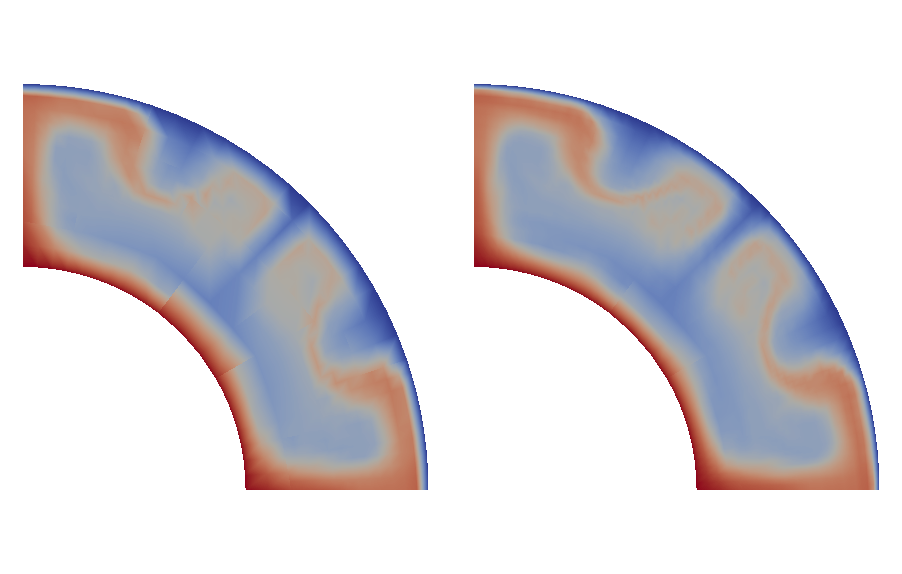
\includegraphics[width=0.5\textwidth]{viz/parameters/build-patches}\end{center}Here, the left picture shows one visualization cell per computational cell (i.e., the option is switch off, as is the default), and the right picture shows the same simulation with the option switched on. The images show the same data, demonstrating that interpolating the solution onto bilinear shape functions as is commonly done in visualizing data loses information.

Of course, activating this option also greatly increases the amount of data \aspect{} will write to disk: approximately by a factor of 4 in 2d, and a factor of 8 in 3d, when using quadratic elements for the velocity, and correspondingly more for even higher order elements.


{\it Possible values:} A boolean value (true or false)
\item {\it Parameter name:} {\tt List of output variables}
\phantomsection\label{parameters:Postprocess/Visualization/List of output variables}


\index[prmindex]{List of output variables}
\index[prmindexfull]{Postprocess!Visualization!List of output variables}
{\it Value:} 


{\it Default:} 


{\it Description:} A comma separated list of visualization objects that should be run whenever writing graphical output. By default, the graphical output files will always contain the primary variables velocity, pressure, and temperature. However, one frequently wants to also visualize derived quantities, such as the thermodynamic phase that corresponds to a given temperature-pressure value, or the corresponding seismic wave speeds. The visualization objects do exactly this: they compute such derived quantities and place them into the output file. The current parameter is the place where you decide which of these additional output variables you want to have in your output file.

The following postprocessors are available:

`Vp anomaly': A visualization output object that generates output showing the percentage anomaly in the seismic compressional wave speed $V_p$ as a spatially variable function with one value per cell. This anomaly is either shown as a percentage anomaly relative to the reference profile given by adiabatic conditions (with the compositions given by the current composition, such that the reference could potentially change through time), or as a percentage change relative to the laterally averaged velocity at the depth of the cell. This velocity is calculated by linear interpolation between average values calculated within equally thick depth slices. The number of depth slices in the domain is user-defined. Typically, the best results will be obtained if the number of depth slices is balanced between being large enough to capture step changes in velocities, but small enough to maintain a reasonable number of evaluation points per slice. Bear in mind that lateral averaging subsamples the finite element mesh.

`Vs anomaly': A visualization output object that generates output showing the percentage anomaly in the seismic shear wave speed $V_s$ as a spatially variable function with one value per cell. This anomaly is either shown as a percentage anomaly relative to the reference profile given by adiabatic conditions (with the compositions given by the current composition, such that the reference could potentially change through time), or as a percentage change relative to the laterally averaged velocity at the depth of the cell. This velocity is calculated by linear interpolation between average values calculated within equally thick depth slices. The number of depth slices in the domain is user-defined. Typically, the best results will be obtained if the number of depth slices is balanced between being large enough to capture step changes in velocities, but small enough to maintain a reasonable number of evaluation points per slice. Bear in mind that lateral averaging subsamples the finite element mesh.

`adiabat': A visualization output object that generates adiabatic temperature, pressure, density, and density derivative as produced by AdiabaticConditions.

`artificial viscosity': A visualization output object that generates output showing the value of the artificial viscosity on each cell.

`artificial viscosity composition': A visualization output object that generates output showing the value of the artificial viscosity for a compositional field on each cell.

`boundary indicators': A visualization output object that generates output about the used boundary indicators. In a loop over the active cells, if a cell lies at a domain boundary, the boundary indicator of the face along the boundary is requested. In case the cell does not lie along any domain boundary, the cell is assigned the value of the largest used boundary indicator plus one. When a cell is situated in one of the corners of the domain, multiple faces will have a boundary indicator. This postprocessor returns the value of the first face along a boundary that is encountered in a loop over all the faces. 

`compositional vector': A visualization output object that outputs vectors whose components are derived from compositional fields. Input parameters for this postprocessor are defined in section Postprocess/Visualization/Compositional fields as vectors

`density': A visualization output object that generates output for the density.

`depth': A visualization output postprocessor that outputs the depth for all points inside the domain, as determined by the geometry model.

`dynamic topography': A visualization output object that generates output for the dynamic topography at the top and bottom of the model space. The approach to determine the dynamic topography requires us to compute the stress tensor and evaluate the component of it in the direction in which gravity acts. In other words, we compute $\sigma_{rr}={\hat g}^T(2 \eta \varepsilon(\mathbf u)-\frac 13 (\textrm{div}\;\mathbf u)I)\hat g - p_d$ where $\hat g = \mathbf g/\|\mathbf g\|$ is the direction of the gravity vector $\mathbf g$ and $p_d=p-p_a$ is the dynamic pressure computed by subtracting the adiabatic pressure $p_a$ from the total pressure $p$ computed as part of the Stokes solve. From this, the dynamic topography is computed using the formula $h=\frac{\sigma_{rr}}{(\mathbf g \cdot \mathbf n)  \rho}$ where $\rho$ is the density at the cell center. For the bottom surface we chose the convection that positive values are up (out) and negative values are in (down), analogous to the deformation of the upper surface. Note that this implementation takes the direction of gravity into account, which means that reversing the flow in backward advection calculations will not reverse the instantaneous topography because the reverse flow will be divided by the reverse surface gravity.

Strictly speaking, the dynamic topography is of course a quantity that is only of interest at the surface. However, we compute it everywhere to make things fit into the framework within which we produce data for visualization. You probably only want to visualize whatever data this postprocessor generates at the surface of your domain and simply ignore the rest of the data generated.

`error indicator': A visualization output object that generates output showing the estimated error or other mesh refinement indicator as a spatially variable function with one value per cell.

`friction heating': A visualization output object that generates output for the amount of friction heating often referred to as $\tau:\epsilon$. More concisely, in the incompressible case, the quantity that is output is defined as $\eta \varepsilon(\mathbf u):\varepsilon(\mathbf u)$ where $\eta$ is itself a function of temperature, pressure and strain rate. In the compressible case, the quantity that is computed is $\eta [\varepsilon(\mathbf u)-\tfrac 13(\textrm{tr}\;\varepsilon(\mathbf u))\mathbf I]:[\varepsilon(\mathbf u)-\tfrac 13(\textrm{tr}\;\varepsilon(\mathbf u))\mathbf I]$.

`geoid': Visualization for the geoid solution. The geoid is given by the equivalent water column height due to a gravity perturbation. (Units: m)

`gravity': A visualization output object that outputs the gravity vector.

`heat flux map': A visualization output object that generates output for the heat flux density across each boundary. The heat flux density is computed in outward direction, i.e., from the domain to the outside, using the formula $-k \nabla T \cdot \mathbf n$, where $k$ is the thermal conductivity as reported by the material model, $T$ is the temperature, and $\mathbf n$ is the outward normal. Note that the quantity so computed does not include any energy transported across the boundary by material transport in cases where $\mathbf u \cdot \mathbf n \neq 0$.At the edge of the domain (e.g. top left corner) the heat flux density is calculated as the sum of the heat flux across both boundaries of the cell (e.g. top and left boundary) divided by the sum of both face areas. The integrated heatflux for each boundary can be obtained from the heat flux statistics postprocessor.

`heating': A visualization output object that generates output for all the heating terms used in the energy equation.

`material properties': A visualization output object that generates output for the material properties given by the material model.There are a number of other visualization postprocessors that offer to write individual material properties. However, they all individually have to evaluate the material model. This is inefficient if one wants to output more than just one or two of the fields provided by the material model. The current postprocessor allows to output a (potentially large) subset of all of the information provided by material models at once, with just a single material model evaluation per output point.

`maximum horizontal compressive stress': A plugin that computes the direction and magnitude of the maximum horizontal component of the compressive stress as a vector field. The direction of this vector can often be used to visualize the principal mode of deformation (e.g., at normal faults or extensional margins) and can be correlated with seismic anisotropy. Recall that the \textit{compressive} stress is simply the negative stress, $\sigma_c=-\sigma=-\left[     2\eta (\varepsilon(\mathbf u)             - \frac 13 (\nabla \cdot \mathbf u) I)     + pI\right]$.

Following \cite{LundTownend07}, we define the maximum horizontal stress direction as that \textit{horizontal} direction $\mathbf n$ that maximizes $\mathbf n^T \sigma_c \mathbf n$. We call a vector \textit{horizontal} if it is perpendicular to the gravity vector $\mathbf g$.

In two space dimensions, $\mathbf n$ is simply a vector that is horizontal (we choose one of the two possible choices). This direction is then scaled by the size of the horizontal stress in this direction, i.e., the plugin outputs the vector $\mathbf w = (\mathbf n^T \sigma_c \mathbf n) \; \mathbf n$.

In three space dimensions, given two horizontal, perpendicular, unit length, but otherwise arbitrarily chosen vectors $\mathbf u,\mathbf v$, we can express $\mathbf n = (\cos \alpha)\mathbf u + (\sin\alpha)\mathbf v$ where $\alpha$ maximizes the expression \begin{align*}  f(\alpha) = \mathbf n^T \sigma_c \mathbf n  = (\mathbf u^T \sigma_c \mathbf u)(\cos\alpha)^2    +2(\mathbf u^T \sigma_c \mathbf v)(\cos\alpha)(\sin\alpha)    +(\mathbf v^T \sigma_c \mathbf v)(\sin\alpha)^2.\end{align*}

The maximum of $f(\alpha)$ is attained where $f'(\alpha)=0$. Evaluating the derivative and using trigonometric identities, one finds that $\alpha$ has to satisfy the equation \begin{align*}  \tan(2\alpha) = \frac{\mathbf u^T \sigma_c \mathbf v}                          {\mathbf u^T \sigma_c \mathbf u                            - \mathbf v^T \sigma_c \mathbf v}.\end{align*}Since the transform $\alpha\mapsto\alpha+\pi$ flips the direction of $\mathbf n$, we only need to seek a solution to this equation in the interval $\alpha\in[0,\pi)$. These are given by $\alpha_1=\frac 12 \arctan \frac{\mathbf u^T \sigma_c \mathbf v}{\mathbf u^T \sigma_c \mathbf u - \mathbf v^T \sigma_c \mathbf v}$ and $\alpha_2=\alpha_1+\frac{\pi}{2}$, one of which will correspond to a minimum and the other to a maximum of $f(\alpha)$. One checks the sign of $f''(\alpha)=-2(\mathbf u^T \sigma_c \mathbf u - \mathbf v^T \sigma_c \mathbf v)\cos(2\alpha) - 2 (\mathbf u^T \sigma_c \mathbf v) \sin(2\alpha)$ for each of these to determine the $\alpha$ that maximizes $f(\alpha)$, and from this immediately arrives at the correct form for the maximum horizontal stress $\mathbf n$.

The description above computes a 3d \textit{direction} vector $\mathbf n$. If one were to scale this vector the same way as done in 2d, i.e., with the magnitude of the stress in this direction, one will typically get vectors whose length is principally determined by the hydrostatic pressure at a given location simply because the hydrostatic pressure is the largest component of the overall stress. On the other hand, the hydrostatic pressure does not determine any principle direction because it is an isotropic, anti-compressive force. As a consequence, there are often points in simulations (e.g., at the center of convection rolls) where the stress has no dominant horizontal direction, and the algorithm above will then in essence choose a random direction because the stress is approximately equal in all horizontal directions. If one scaled the output by the magnitude of the stress in this direction (i.e., approximately equal to the hydrostatic pressure at this point), one would get randomly oriented vectors at these locations with significant lengths.

To avoid this problem, we scale the maximal horizontal compressive stress direction $\mathbf n$ by the \textit{difference} between the stress in the maximal and minimal horizontal stress directions. In other words, let $\mathbf n_\perp=(\sin \alpha)\mathbf u - (\cos\alpha)\mathbf v$ be the horizontal direction perpendicular to $\mathbf n$, then this plugin outputs the vector quantity $\mathbf w = (\mathbf n^T \sigma_c \mathbf n                -\mathbf n^T_\perp \sigma_c \mathbf n_\perp)               \; \mathbf n$. In other words, the length of the vector produced indicates \textit{how dominant} the direction of maximal horizontal compressive strength is.

Fig.~\ref{fig:max-horizontal-compressive-stress} shows a simple example for this kind of visualization in 3d.

\begin{figure}  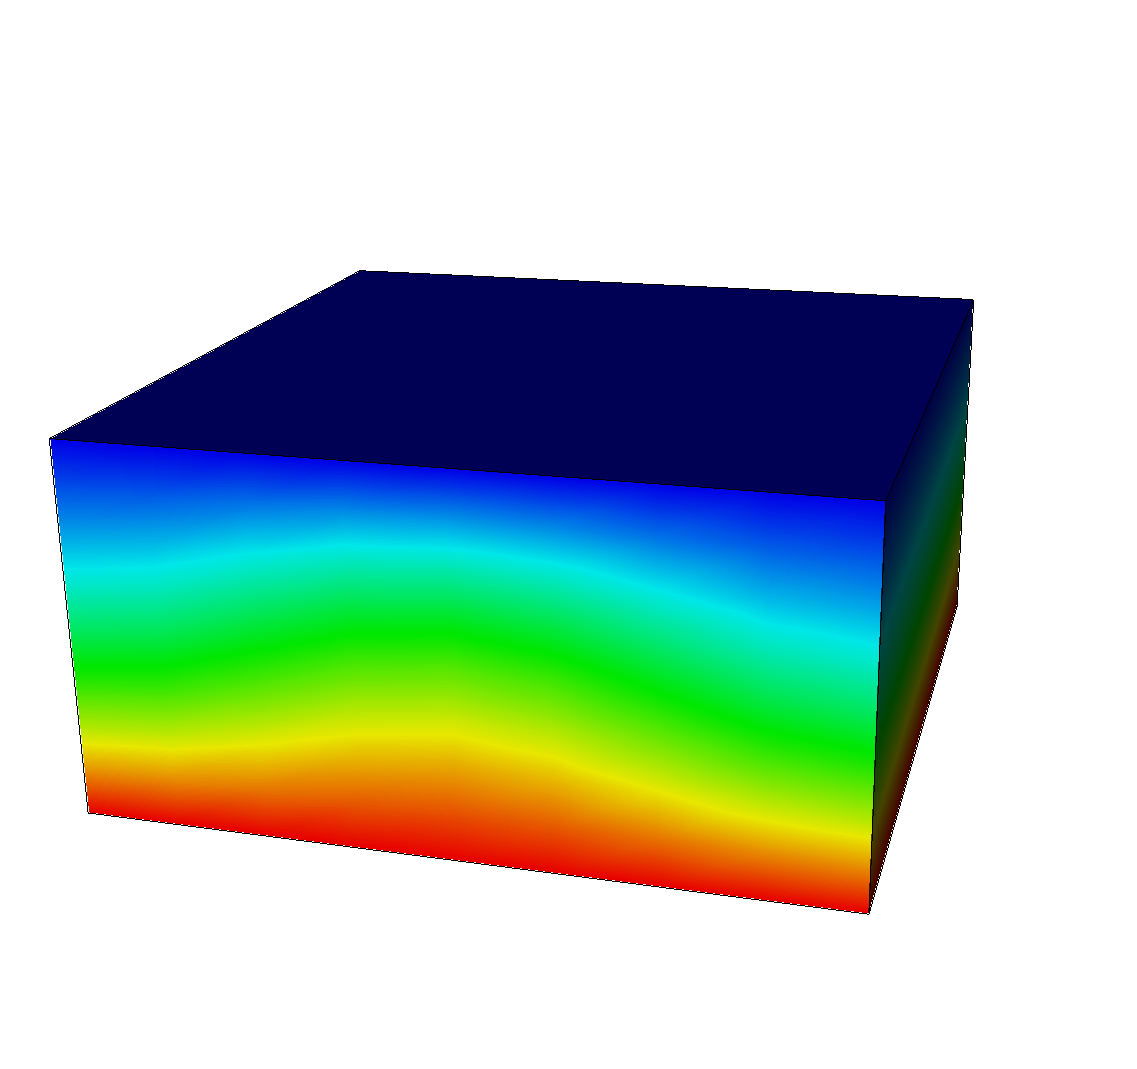
\includegraphics[width=0.3\textwidth]    {viz/plugins/maximum_horizontal_compressive_stress/temperature.png}  \hfill  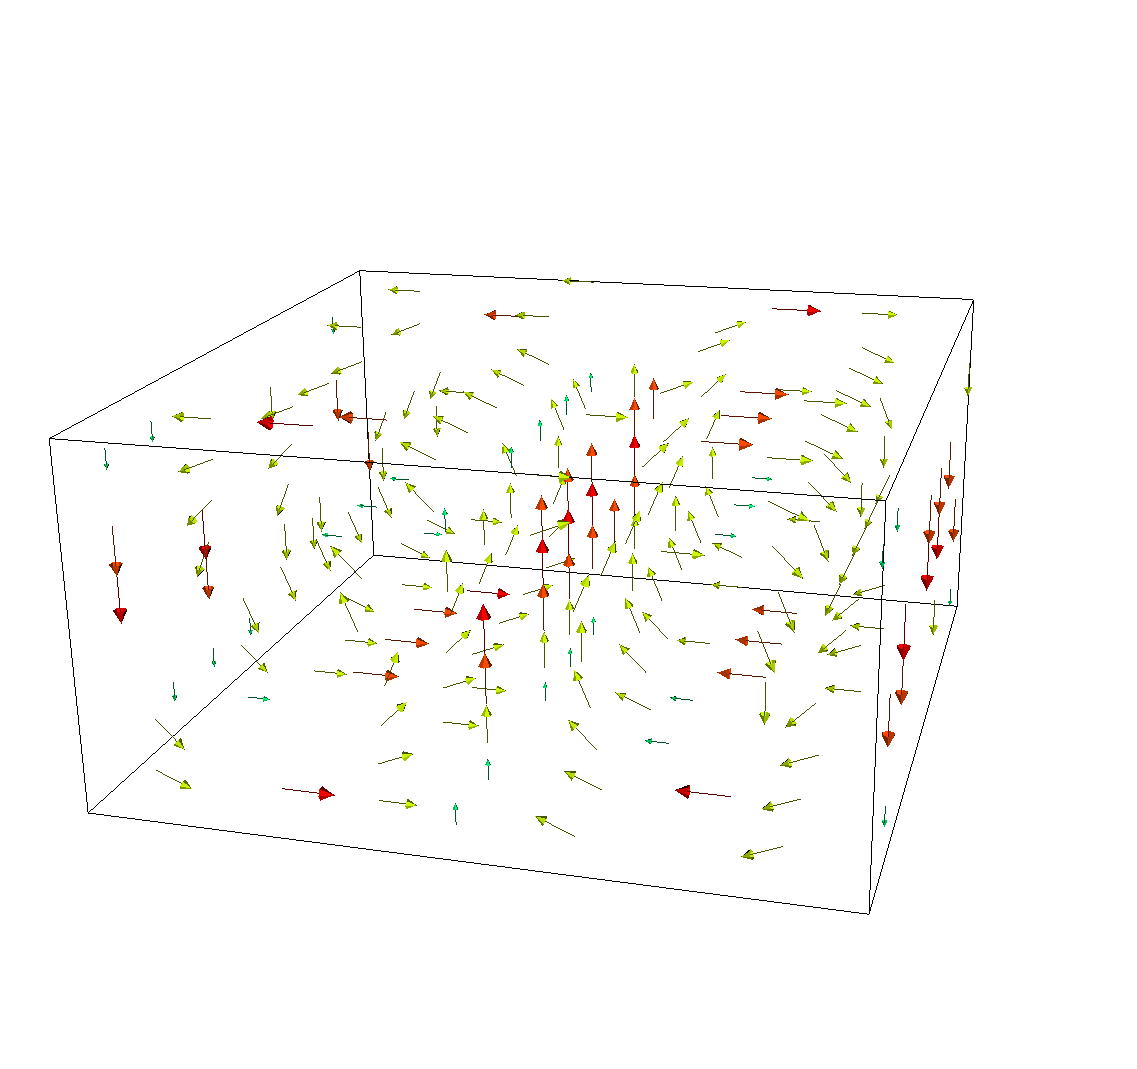
\includegraphics[width=0.3\textwidth]    {viz/plugins/maximum_horizontal_compressive_stress/velocity.png}  \hfill  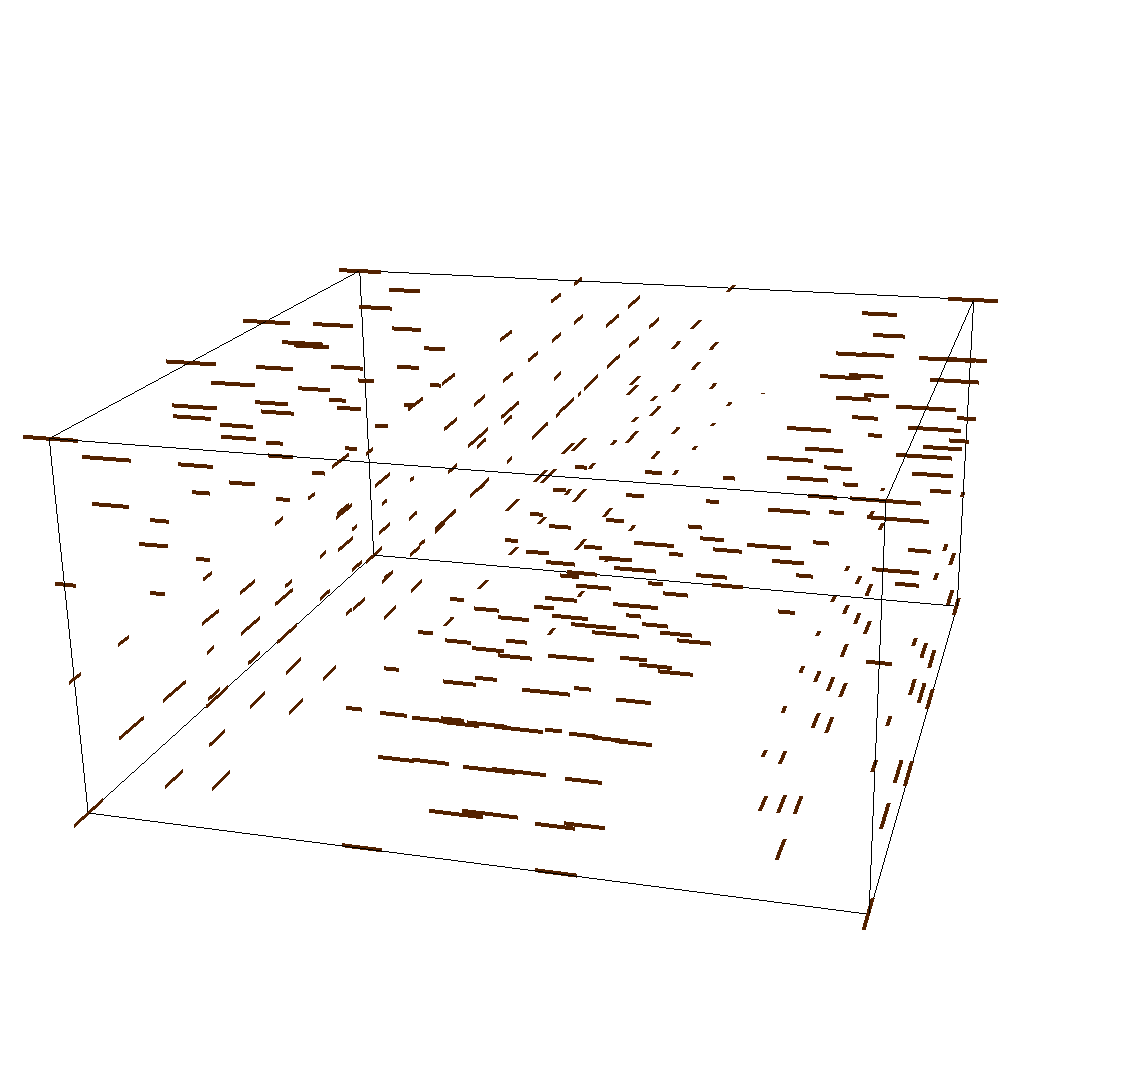
\includegraphics[width=0.3\textwidth]    {viz/plugins/maximum_horizontal_compressive_stress/horizontal-stress.png}  \caption{\it Illustration of the `maximum horizontal     compressive stress' visualization plugin. The left     figure shows a ridge-like temperature anomaly. Together     with no-slip boundary along all six boundaries, this     results in two convection rolls (center). The maximal     horizontal compressive strength at the bottom center     of the domain is perpendicular to the ridge because     the flow comes together there from the left and right,     yielding a compressive force in left-right direction.     At the top of the model, the flow separates outward,     leading to a \textit{negative} compressive stress     in left-right direction; because there is no flow     in front-back direction, the compressive strength     in front-back direction is zero, making the along-ridge     direction the dominant one. At the center of the     convection rolls, both horizontal directions yield     the same stress; the plugin therefore chooses an     essentially arbitrary horizontal vector, but then     uses a zero magnitude given that the difference     between the maximal and minimal horizontal stress     is zero at these points.}  \label{fig:max-horizontal-compressive-stress}\end{figure}

`melt fraction': A visualization output object that generates output for the melt fraction at the temperature and pressure of the current point. If the material model computes a melt fraction, this is the quantity that will be visualized. Otherwise, a specific parametrization for batch melting (as described in the following) will be used. It does not take into account latent heat. If there are no compositional fields, this postprocessor will visualize the melt fraction of peridotite (calculated using the anhydrous model of Katz, 2003). If there is at least one compositional field, the postprocessor assumes that the  first compositional field is the content of pyroxenite, and will visualize the melt fraction for a mixture of peridotite and pyroxenite (using the melting model of Sobolev, 2011 for pyroxenite). All the parameters that were used in these calculations can be changed in the input file, the most relevant maybe being the mass fraction of Cpx in peridotite in the Katz melting model (Mass fraction cpx), which right now has a default of 15\%. The corresponding p-T-diagrams can be generated by running the tests melt\_postprocessor\_peridotite and melt\_postprocessor\_pyroxenite.

`melt material properties': A visualization output object that generates output for melt related properties of the material model.

`named additional outputs': Some material models can compute quantities other than those that typically appear in the equations that \aspect{} solves (such as the viscosity, density, etc). Examples of quantities material models may be able to compute are seismic velocities, or other quantities that can be derived from the state variables and the material coefficients such as the stress or stress anisotropies. These quantities are generically referred to as `named outputs' because they are given an explicit name different from the usual outputs of material models.

This visualization postprocessor outputs whatever quantities the material model can compute. What quantities these are is specific to the material model in use for a simulation, and for many models in fact does not contain any named outputs at all.

`nonadiabatic pressure': A visualization output object that generates output for the non-adiabatic component of the pressure.

`nonadiabatic temperature': A visualization output object that generates output for the non-adiabatic component of the pressure.

`particle count': A visualization output object that generates output about the number of particles per cell.

`partition': A visualization output object that generates output for the parallel partition that every cell of the mesh is associated with.

`shear stress': A visualization output object that generates output for the 3 (in 2d) or 6 (in 3d) components of the shear stress tensor, i.e., for the components of the tensor $2\eta\varepsilon(\mathbf u)$ in the incompressible case and $2\eta\left[\varepsilon(\mathbf u)-\tfrac 13(\textrm{tr}\;\varepsilon(\mathbf u))\mathbf I\right]$ in the compressible case. The shear stress differs from the full stress tensor by the absence of the pressure.

`spd factor': A visualization output object that generates output for the spd factor. The spd factor is a factor which scales a part of the Jacobian used for the Newton solver to make sure that the Jacobian remains positive definite.

`specific heat': A visualization output object that generates output for the specific heat $C_p$.

`strain rate': A visualization output object that generates output for the norm of the strain rate, i.e., for the quantity $\sqrt{\varepsilon(\mathbf u):\varepsilon(\mathbf u)}$ in the incompressible case and $\sqrt{[\varepsilon(\mathbf u)-\tfrac 13(\textrm{tr}\;\varepsilon(\mathbf u))\mathbf I]:[\varepsilon(\mathbf u)-\tfrac 13(\textrm{tr}\;\varepsilon(\mathbf u))\mathbf I]}$ in the compressible case.

`stress': A visualization output object that generates output for the 3 (in 2d) or 6 (in 3d) components of the stress tensor, i.e., for the components of the tensor $2\eta\varepsilon(\mathbf u)+pI$ in the incompressible case and $2\eta\left[\varepsilon(\mathbf u)-\tfrac 13(\textrm{tr}\;\varepsilon(\mathbf u))\mathbf I\right]+pI$ in the compressible case.

`thermal conductivity': A visualization output object that generates output for the thermal conductivity $k$.

`thermal diffusivity': A visualization output object that generates output for the thermal diffusivity $\kappa$=$\frac{k}{\rho C_p}$, with $k$ the thermal conductivity.

`thermal expansivity': A visualization output object that generates output for the thermal expansivity.

`vertical heat flux': A visualization output object that generates output for the heat flux in the vertical direction, which is the sum of the advective and the conductive heat flux, with the sign convention of positive flux upwards.

`viscosity': A visualization output object that generates output for the viscosity.

`volumetric strain rate': A visualization output object that generates output for the volumetric strain rate, i.e., for the quantity $\nabla\cdot\mathbf u = \textrm{div}\; \mathbf u = \textrm{trace}\; \varepsilon(\mathbf u)$. This should be zero (in some average sense) in incompressible convection models, but can be non-zero in compressible models and models with melt transport.


{\it Possible values:} A comma-separated list of any of Vp anomaly, Vs anomaly, adiabat, artificial viscosity, artificial viscosity composition, boundary indicators, compositional vector, density, depth, dynamic topography, error indicator, friction heating, geoid, gravity, heat flux map, heating, material properties, maximum horizontal compressive stress, melt fraction, melt material properties, named additional outputs, nonadiabatic pressure, nonadiabatic temperature, particle count, partition, shear stress, spd factor, specific heat, strain rate, stress, thermal conductivity, thermal diffusivity, thermal expansivity, vertical heat flux, viscosity, volumetric strain rate
\item {\it Parameter name:} {\tt Number of grouped files}
\phantomsection\label{parameters:Postprocess/Visualization/Number of grouped files}


\index[prmindex]{Number of grouped files}
\index[prmindexfull]{Postprocess!Visualization!Number of grouped files}
{\it Value:} 16


{\it Default:} 16


{\it Description:} VTU file output supports grouping files from several CPUs into a given number of files using MPI I/O when writing on a parallel filesystem. Select 0 for no grouping. This will disable parallel file output and instead write one file per processor. A value of 1 will generate one big file containing the whole solution, while a larger value will create that many files (at most as many as there are MPI ranks).


{\it Possible values:} An integer $n$ such that $0\leq n \leq 2147483647$
\item {\it Parameter name:} {\tt Output format}
\phantomsection\label{parameters:Postprocess/Visualization/Output format}


\index[prmindex]{Output format}
\index[prmindexfull]{Postprocess!Visualization!Output format}
{\it Value:} vtu


{\it Default:} vtu


{\it Description:} The file format to be used for graphical output.


{\it Possible values:} Any one of none, dx, ucd, gnuplot, povray, eps, gmv, tecplot, tecplot\_binary, vtk, vtu, hdf5, svg, deal.II intermediate
\item {\it Parameter name:} {\tt Output mesh velocity}
\phantomsection\label{parameters:Postprocess/Visualization/Output mesh velocity}


\index[prmindex]{Output mesh velocity}
\index[prmindexfull]{Postprocess!Visualization!Output mesh velocity}
{\it Value:} false


{\it Default:} false


{\it Description:} For free surface computations Aspect uses an Arbitrary-Lagrangian-Eulerian formulation to handle deforming the domain, so the mesh has its own velocity field.  This may be written as an output field by setting this parameter to true.


{\it Possible values:} A boolean value (true or false)
\item {\it Parameter name:} {\tt Temporary output location}
\phantomsection\label{parameters:Postprocess/Visualization/Temporary output location}


\index[prmindex]{Temporary output location}
\index[prmindexfull]{Postprocess!Visualization!Temporary output location}
{\it Value:} 


{\it Default:} 


{\it Description:} On large clusters it can be advantageous to first write the output to a temporary file on a local file system and later move this file to a network file system. If this variable is set to a non-empty string it will be interpreted as a temporary storage location.


{\it Possible values:} Any string
\item {\it Parameter name:} {\tt Time between graphical output}
\phantomsection\label{parameters:Postprocess/Visualization/Time between graphical output}


\index[prmindex]{Time between graphical output}
\index[prmindexfull]{Postprocess!Visualization!Time between graphical output}
{\it Value:} 1e8


{\it Default:} 1e8


{\it Description:} The time interval between each generation of graphical output files. A value of zero indicates that output should be generated in each time step. Units: years if the 'Use years in output instead of seconds' parameter is set; seconds otherwise.


{\it Possible values:} A floating point number $v$ such that $0 \leq v \leq \text{MAX\_DOUBLE}$
\item {\it Parameter name:} {\tt Write in background thread}
\phantomsection\label{parameters:Postprocess/Visualization/Write in background thread}


\index[prmindex]{Write in background thread}
\index[prmindexfull]{Postprocess!Visualization!Write in background thread}
{\it Value:} false


{\it Default:} false


{\it Description:} File operations can potentially take a long time, blocking the progress of the rest of the model run. Setting this variable to `true' moves this process into a background thread, while the rest of the model continues.


{\it Possible values:} A boolean value (true or false)
\end{itemize}



\subsection{Parameters in section \tt Postprocess/Visualization/Artificial viscosity composition}
\label{parameters:Postprocess/Visualization/Artificial_20viscosity_20composition}

\begin{itemize}
\item {\it Parameter name:} {\tt Name of compositional field}
\phantomsection\label{parameters:Postprocess/Visualization/Artificial viscosity composition/Name of compositional field}


\index[prmindex]{Name of compositional field}
\index[prmindexfull]{Postprocess!Visualization!Artificial viscosity composition/Name of compositional field}
{\it Value:} 


{\it Default:} 


{\it Description:} The name of the compositional field whose output should be visualized. 


{\it Possible values:} Any string
\end{itemize}

\subsection{Parameters in section \tt Postprocess/Visualization/Compositional fields as vectors}
\label{parameters:Postprocess/Visualization/Compositional_20fields_20as_20vectors}

\begin{itemize}
\item {\it Parameter name:} {\tt Names of fields}
\phantomsection\label{parameters:Postprocess/Visualization/Compositional fields as vectors/Names of fields}


\index[prmindex]{Names of fields}
\index[prmindexfull]{Postprocess!Visualization!Compositional fields as vectors/Names of fields}
{\it Value:} 


{\it Default:} 


{\it Description:} A list of sets of compositional fields which should be output as vectors. Sets are separated from each other by semicolons and vector components within each set are separated by commas (e.g. $vec1_x$, $vec1_y$ ; $vec2_x$, $vec2_y$) where each name must be a defined named compositional field. If only one name is given in a set, it is interpreted as the first in a sequence of dim consecutive compositional fields.


{\it Possible values:} Any string
\item {\it Parameter name:} {\tt Names of vectors}
\phantomsection\label{parameters:Postprocess/Visualization/Compositional fields as vectors/Names of vectors}


\index[prmindex]{Names of vectors}
\index[prmindexfull]{Postprocess!Visualization!Compositional fields as vectors/Names of vectors}
{\it Value:} 


{\it Default:} 


{\it Description:} Names of vectors as they will appear in the output.


{\it Possible values:} A list of 0 to 4294967295 elements where each element is [Any string]
\end{itemize}

\subsection{Parameters in section \tt Postprocess/Visualization/Material properties}
\label{parameters:Postprocess/Visualization/Material_20properties}

\begin{itemize}
\item {\it Parameter name:} {\tt List of material properties}
\phantomsection\label{parameters:Postprocess/Visualization/Material properties/List of material properties}


\index[prmindex]{List of material properties}
\index[prmindexfull]{Postprocess!Visualization!Material properties/List of material properties}
{\it Value:} density,thermal expansivity,specific heat,viscosity


{\it Default:} density,thermal expansivity,specific heat,viscosity


{\it Description:} A comma separated list of material properties that should be written whenever writing graphical output. By default, the material properties will always contain the density, thermal expansivity, specific heat and viscosity. The following material properties are available:

viscosity|density|thermal expansivity|specific heat|thermal conductivity|thermal diffusivity|compressibility|entropy derivative temperature|entropy derivative pressure|reaction terms|melt fraction


{\it Possible values:} A comma-separated list of any of viscosity, density, thermal expansivity, specific heat, thermal conductivity, thermal diffusivity, compressibility, entropy derivative temperature, entropy derivative pressure, reaction terms, melt fraction
\end{itemize}

\subsection{Parameters in section \tt Postprocess/Visualization/Melt fraction}
\label{parameters:Postprocess/Visualization/Melt_20fraction}

\begin{itemize}
\item {\it Parameter name:} {\tt A1}
\phantomsection\label{parameters:Postprocess/Visualization/Melt fraction/A1}


\index[prmindex]{A1}
\index[prmindexfull]{Postprocess!Visualization!Melt fraction/A1}
{\it Value:} 1085.7


{\it Default:} 1085.7


{\it Description:} Constant parameter in the quadratic function that approximates the solidus of peridotite. Units: $°C$.


{\it Possible values:} A floating point number $v$ such that $-\text{MAX\_DOUBLE} \leq v \leq \text{MAX\_DOUBLE}$
\item {\it Parameter name:} {\tt A2}
\phantomsection\label{parameters:Postprocess/Visualization/Melt fraction/A2}


\index[prmindex]{A2}
\index[prmindexfull]{Postprocess!Visualization!Melt fraction/A2}
{\it Value:} 1.329e-7


{\it Default:} 1.329e-7


{\it Description:} Prefactor of the linear pressure term in the quadratic function that approximates the solidus of peridotite. Units: $°C/Pa$.


{\it Possible values:} A floating point number $v$ such that $-\text{MAX\_DOUBLE} \leq v \leq \text{MAX\_DOUBLE}$
\item {\it Parameter name:} {\tt A3}
\phantomsection\label{parameters:Postprocess/Visualization/Melt fraction/A3}


\index[prmindex]{A3}
\index[prmindexfull]{Postprocess!Visualization!Melt fraction/A3}
{\it Value:} -5.1e-18


{\it Default:} -5.1e-18


{\it Description:} Prefactor of the quadratic pressure term in the quadratic function that approximates the solidus of peridotite. Units: $°C/(Pa^2)$.


{\it Possible values:} A floating point number $v$ such that $-\text{MAX\_DOUBLE} \leq v \leq \text{MAX\_DOUBLE}$
\item {\it Parameter name:} {\tt B1}
\phantomsection\label{parameters:Postprocess/Visualization/Melt fraction/B1}


\index[prmindex]{B1}
\index[prmindexfull]{Postprocess!Visualization!Melt fraction/B1}
{\it Value:} 1475.0


{\it Default:} 1475.0


{\it Description:} Constant parameter in the quadratic function that approximates the lherzolite liquidus used for calculating the fraction of peridotite-derived melt. Units: $°C$.


{\it Possible values:} A floating point number $v$ such that $-\text{MAX\_DOUBLE} \leq v \leq \text{MAX\_DOUBLE}$
\item {\it Parameter name:} {\tt B2}
\phantomsection\label{parameters:Postprocess/Visualization/Melt fraction/B2}


\index[prmindex]{B2}
\index[prmindexfull]{Postprocess!Visualization!Melt fraction/B2}
{\it Value:} 8.0e-8


{\it Default:} 8.0e-8


{\it Description:} Prefactor of the linear pressure term in the quadratic function that approximates the  lherzolite liquidus used for calculating the fraction of peridotite-derived melt. Units: $°C/Pa$.


{\it Possible values:} A floating point number $v$ such that $-\text{MAX\_DOUBLE} \leq v \leq \text{MAX\_DOUBLE}$
\item {\it Parameter name:} {\tt B3}
\phantomsection\label{parameters:Postprocess/Visualization/Melt fraction/B3}


\index[prmindex]{B3}
\index[prmindexfull]{Postprocess!Visualization!Melt fraction/B3}
{\it Value:} -3.2e-18


{\it Default:} -3.2e-18


{\it Description:} Prefactor of the quadratic pressure term in the quadratic function that approximates the  lherzolite liquidus used for calculating the fraction of peridotite-derived melt. Units: $°C/(Pa^2)$.


{\it Possible values:} A floating point number $v$ such that $-\text{MAX\_DOUBLE} \leq v \leq \text{MAX\_DOUBLE}$
\item {\it Parameter name:} {\tt C1}
\phantomsection\label{parameters:Postprocess/Visualization/Melt fraction/C1}


\index[prmindex]{C1}
\index[prmindexfull]{Postprocess!Visualization!Melt fraction/C1}
{\it Value:} 1780.0


{\it Default:} 1780.0


{\it Description:} Constant parameter in the quadratic function that approximates the liquidus of peridotite. Units: $°C$.


{\it Possible values:} A floating point number $v$ such that $-\text{MAX\_DOUBLE} \leq v \leq \text{MAX\_DOUBLE}$
\item {\it Parameter name:} {\tt C2}
\phantomsection\label{parameters:Postprocess/Visualization/Melt fraction/C2}


\index[prmindex]{C2}
\index[prmindexfull]{Postprocess!Visualization!Melt fraction/C2}
{\it Value:} 4.50e-8


{\it Default:} 4.50e-8


{\it Description:} Prefactor of the linear pressure term in the quadratic function that approximates the liquidus of peridotite. Units: $°C/Pa$.


{\it Possible values:} A floating point number $v$ such that $-\text{MAX\_DOUBLE} \leq v \leq \text{MAX\_DOUBLE}$
\item {\it Parameter name:} {\tt C3}
\phantomsection\label{parameters:Postprocess/Visualization/Melt fraction/C3}


\index[prmindex]{C3}
\index[prmindexfull]{Postprocess!Visualization!Melt fraction/C3}
{\it Value:} -2.0e-18


{\it Default:} -2.0e-18


{\it Description:} Prefactor of the quadratic pressure term in the quadratic function that approximates the liquidus of peridotite. Units: $°C/(Pa^2)$.


{\it Possible values:} A floating point number $v$ such that $-\text{MAX\_DOUBLE} \leq v \leq \text{MAX\_DOUBLE}$
\item {\it Parameter name:} {\tt D1}
\phantomsection\label{parameters:Postprocess/Visualization/Melt fraction/D1}


\index[prmindex]{D1}
\index[prmindexfull]{Postprocess!Visualization!Melt fraction/D1}
{\it Value:} 976.0


{\it Default:} 976.0


{\it Description:} Constant parameter in the quadratic function that approximates the solidus of pyroxenite. Units: $°C$.


{\it Possible values:} A floating point number $v$ such that $-\text{MAX\_DOUBLE} \leq v \leq \text{MAX\_DOUBLE}$
\item {\it Parameter name:} {\tt D2}
\phantomsection\label{parameters:Postprocess/Visualization/Melt fraction/D2}


\index[prmindex]{D2}
\index[prmindexfull]{Postprocess!Visualization!Melt fraction/D2}
{\it Value:} 1.329e-7


{\it Default:} 1.329e-7


{\it Description:} Prefactor of the linear pressure term in the quadratic function that approximates the solidus of pyroxenite. Note that this factor is different from the value given in Sobolev, 2011, because they use the potential temperature whereas we use the absolute temperature. Units: $°C/Pa$.


{\it Possible values:} A floating point number $v$ such that $-\text{MAX\_DOUBLE} \leq v \leq \text{MAX\_DOUBLE}$
\item {\it Parameter name:} {\tt D3}
\phantomsection\label{parameters:Postprocess/Visualization/Melt fraction/D3}


\index[prmindex]{D3}
\index[prmindexfull]{Postprocess!Visualization!Melt fraction/D3}
{\it Value:} -5.1e-18


{\it Default:} -5.1e-18


{\it Description:} Prefactor of the quadratic pressure term in the quadratic function that approximates the solidus of pyroxenite. Units: $°C/(Pa^2)$.


{\it Possible values:} A floating point number $v$ such that $-\text{MAX\_DOUBLE} \leq v \leq \text{MAX\_DOUBLE}$
\item {\it Parameter name:} {\tt E1}
\phantomsection\label{parameters:Postprocess/Visualization/Melt fraction/E1}


\index[prmindex]{E1}
\index[prmindexfull]{Postprocess!Visualization!Melt fraction/E1}
{\it Value:} 663.8


{\it Default:} 663.8


{\it Description:} Prefactor of the linear depletion term in the quadratic function that approximates the melt fraction of pyroxenite. Units: $°C/Pa$.


{\it Possible values:} A floating point number $v$ such that $-\text{MAX\_DOUBLE} \leq v \leq \text{MAX\_DOUBLE}$
\item {\it Parameter name:} {\tt E2}
\phantomsection\label{parameters:Postprocess/Visualization/Melt fraction/E2}


\index[prmindex]{E2}
\index[prmindexfull]{Postprocess!Visualization!Melt fraction/E2}
{\it Value:} -611.4


{\it Default:} -611.4


{\it Description:} Prefactor of the quadratic depletion term in the quadratic function that approximates the melt fraction of pyroxenite. Units: $°C/(Pa^2)$.


{\it Possible values:} A floating point number $v$ such that $-\text{MAX\_DOUBLE} \leq v \leq \text{MAX\_DOUBLE}$
\item {\it Parameter name:} {\tt Mass fraction cpx}
\phantomsection\label{parameters:Postprocess/Visualization/Melt fraction/Mass fraction cpx}


\index[prmindex]{Mass fraction cpx}
\index[prmindexfull]{Postprocess!Visualization!Melt fraction/Mass fraction cpx}
{\it Value:} 0.15


{\it Default:} 0.15


{\it Description:} Mass fraction of clinopyroxene in the peridotite to be molten. Units: non-dimensional.


{\it Possible values:} A floating point number $v$ such that $-\text{MAX\_DOUBLE} \leq v \leq \text{MAX\_DOUBLE}$
\item {\it Parameter name:} {\tt beta}
\phantomsection\label{parameters:Postprocess/Visualization/Melt fraction/beta}


\index[prmindex]{beta}
\index[prmindexfull]{Postprocess!Visualization!Melt fraction/beta}
{\it Value:} 1.5


{\it Default:} 1.5


{\it Description:} Exponent of the melting temperature in the melt fraction calculation. Units: non-dimensional.


{\it Possible values:} A floating point number $v$ such that $-\text{MAX\_DOUBLE} \leq v \leq \text{MAX\_DOUBLE}$
\item {\it Parameter name:} {\tt r1}
\phantomsection\label{parameters:Postprocess/Visualization/Melt fraction/r1}


\index[prmindex]{r1}
\index[prmindexfull]{Postprocess!Visualization!Melt fraction/r1}
{\it Value:} 0.5


{\it Default:} 0.5


{\it Description:} Constant in the linear function that approximates the clinopyroxene reaction coefficient. Units: non-dimensional.


{\it Possible values:} A floating point number $v$ such that $-\text{MAX\_DOUBLE} \leq v \leq \text{MAX\_DOUBLE}$
\item {\it Parameter name:} {\tt r2}
\phantomsection\label{parameters:Postprocess/Visualization/Melt fraction/r2}


\index[prmindex]{r2}
\index[prmindexfull]{Postprocess!Visualization!Melt fraction/r2}
{\it Value:} 8e-11


{\it Default:} 8e-11


{\it Description:} Prefactor of the linear pressure term in the linear function that approximates the clinopyroxene reaction coefficient. Units: $1/Pa$.


{\it Possible values:} A floating point number $v$ such that $-\text{MAX\_DOUBLE} \leq v \leq \text{MAX\_DOUBLE}$
\end{itemize}

\subsection{Parameters in section \tt Postprocess/Visualization/Melt material properties}
\label{parameters:Postprocess/Visualization/Melt_20material_20properties}

\begin{itemize}
\item {\it Parameter name:} {\tt List of properties}
\phantomsection\label{parameters:Postprocess/Visualization/Melt material properties/List of properties}


\index[prmindex]{List of properties}
\index[prmindexfull]{Postprocess!Visualization!Melt material properties/List of properties}
{\it Value:} compaction viscosity,permeability


{\it Default:} compaction viscosity,permeability


{\it Description:} A comma separated list of melt properties that should be written whenever writing graphical output. The following material properties are available:

compaction viscosity|fluid viscosity|permeability|fluid density|fluid density gradient


{\it Possible values:} A comma-separated list of any of compaction viscosity, fluid viscosity, permeability, fluid density, fluid density gradient
\end{itemize}

\subsection{Parameters in section \tt Postprocess/Visualization/Vp anomaly}
\label{parameters:Postprocess/Visualization/Vp_20anomaly}

\begin{itemize}
\item {\it Parameter name:} {\tt Average velocity scheme}
\phantomsection\label{parameters:Postprocess/Visualization/Vp anomaly/Average velocity scheme}


\index[prmindex]{Average velocity scheme}
\index[prmindexfull]{Postprocess!Visualization!Vp anomaly/Average velocity scheme}
{\it Value:} reference profile


{\it Default:} reference profile


{\it Description:} Scheme to compute the average velocity-depth profile. The reference profile option evaluates the conditions along the reference adiabat according to the material model. The lateral average option instead calculates a lateral average from subdivision of the mesh. The lateral average option may produce spurious results where there are sharp velocity changes.


{\it Possible values:} Any one of reference profile, lateral average
\item {\it Parameter name:} {\tt Number of depth slices}
\phantomsection\label{parameters:Postprocess/Visualization/Vp anomaly/Number of depth slices}


\index[prmindex]{Number of depth slices}
\index[prmindexfull]{Postprocess!Visualization!Vp anomaly/Number of depth slices}
{\it Value:} 50


{\it Default:} 50


{\it Description:} Number of depth slices used to define average seismic compressional wave velocities from which anomalies are calculated. Units: non-dimensional.


{\it Possible values:} An integer $n$ such that $1\leq n \leq 2147483647$
\end{itemize}

\subsection{Parameters in section \tt Postprocess/Visualization/Vs anomaly}
\label{parameters:Postprocess/Visualization/Vs_20anomaly}

\begin{itemize}
\item {\it Parameter name:} {\tt Average velocity scheme}
\phantomsection\label{parameters:Postprocess/Visualization/Vs anomaly/Average velocity scheme}


\index[prmindex]{Average velocity scheme}
\index[prmindexfull]{Postprocess!Visualization!Vs anomaly/Average velocity scheme}
{\it Value:} reference profile


{\it Default:} reference profile


{\it Description:} Scheme to compute the average velocity-depth profile. The reference profile option evaluates the conditions along the reference adiabat according to the material model. The lateral average option instead calculates a lateral average from subdivision of the mesh. The lateral average option may produce spurious results where there are sharp velocity changes.


{\it Possible values:} Any one of reference profile, lateral average
\item {\it Parameter name:} {\tt Number of depth slices}
\phantomsection\label{parameters:Postprocess/Visualization/Vs anomaly/Number of depth slices}


\index[prmindex]{Number of depth slices}
\index[prmindexfull]{Postprocess!Visualization!Vs anomaly/Number of depth slices}
{\it Value:} 50


{\it Default:} 50


{\it Description:} Number of depth slices used to define average seismic shear wave velocities from which anomalies are calculated. Units: non-dimensional.


{\it Possible values:} An integer $n$ such that $1\leq n \leq 2147483647$
\end{itemize}

\subsection{Parameters in section \tt Prescribed Stokes solution}
\label{parameters:Prescribed_20Stokes_20solution}

\begin{itemize}
\item {\it Parameter name:} {\tt Model name}
\phantomsection\label{parameters:Prescribed Stokes solution/Model name}


\index[prmindex]{Model name}
\index[prmindexfull]{Prescribed Stokes solution!Model name}
{\it Value:} unspecified


{\it Default:} unspecified


{\it Description:} Select one of the following models:

`ascii data': Implementation of a model in which the velocity is derived from files containing data in ascii format. Note the required format of the input data: The first lines may contain any number of comments if they begin with '\#', but one of these lines needs to contain the number of grid points in each dimension as for example '\# POINTS: 3 3'. The order of the data columns has to be `x', `y', `v$_x$' , `v$_y$' in a 2d model and  `x', `y', `z', `v$_x$' , `v$_y$' , `v$_z$' in a 3d model. Note that the data in the input files need to be sorted in a specific order: the first coordinate needs to ascend first, followed by the second and the third at last in order to assign the correct data to the prescribed coordinates. If you use a spherical model, then the data will still be handled as Cartesian, however the assumed grid changes. `x' will be replaced by the radial distance of the point to the bottom of the model, `y' by the azimuth angle and `z' by the polar angle measured positive from the north pole. The grid will be assumed to be a latitude-longitude grid. Note that the order of spherical coordinates is `r', `phi', `theta' and not `r', `theta', `phi', since this allows for dimension independent expressions.

`circle': This value describes a vector field that rotates around the z-axis with constant angular velocity (i.e., with a velocity that increases with distance from the axis). The pressure is set to zero.

`function': This plugin allows to prescribe the Stokes solution for the velocity and pressure field in terms of an explicit formula. The format of these functions follows the syntax understood by the muparser library, see Section~\ref{sec:muparser-format}.


{\it Possible values:} Any one of ascii data, circle, function, unspecified
\end{itemize}



\subsection{Parameters in section \tt Prescribed Stokes solution/Ascii data model}
\label{parameters:Prescribed_20Stokes_20solution/Ascii_20data_20model}

\begin{itemize}
\item {\it Parameter name:} {\tt Data directory}
\phantomsection\label{parameters:Prescribed Stokes solution/Ascii data model/Data directory}


\index[prmindex]{Data directory}
\index[prmindexfull]{Prescribed Stokes solution!Ascii data model!Data directory}
{\it Value:} \$ASPECT\_SOURCE\_DIR/data/prescribed-stokes-solution/


{\it Default:} \$ASPECT\_SOURCE\_DIR/data/prescribed-stokes-solution/


{\it Description:} The name of a directory that contains the model data. This path may either be absolute (if starting with a '/') or relative to the current directory. The path may also include the special text '\$ASPECT\_SOURCE\_DIR' which will be interpreted as the path in which the ASPECT source files were located when ASPECT was compiled. This interpretation allows, for example, to reference files located in the `data/' subdirectory of ASPECT. 


{\it Possible values:} A directory name
\item {\it Parameter name:} {\tt Data file name}
\phantomsection\label{parameters:Prescribed Stokes solution/Ascii data model/Data file name}


\index[prmindex]{Data file name}
\index[prmindexfull]{Prescribed Stokes solution!Ascii data model!Data file name}
{\it Value:} box\_2d.txt


{\it Default:} box\_2d.txt


{\it Description:} The file name of the material data. Provide file in format: (Velocity file name).\%s\%d where \%s is a string specifying the boundary of the model according to the names of the boundary indicators (of a box or a spherical shell).\%d is any sprintf integer qualifier, specifying the format of the current file number. 


{\it Possible values:} Any string
\item {\it Parameter name:} {\tt Scale factor}
\phantomsection\label{parameters:Prescribed Stokes solution/Ascii data model/Scale factor}


\index[prmindex]{Scale factor}
\index[prmindexfull]{Prescribed Stokes solution!Ascii data model!Scale factor}
{\it Value:} 1


{\it Default:} 1


{\it Description:} Scalar factor, which is applied to the boundary velocity. You might want to use this to scale the velocities to a reference model (e.g. with free-slip boundary) or another plate reconstruction. Another way to use this factor is to convert units of the input files. The unit is assumed to bem/s or m/yr depending on the 'Use years in output instead of seconds' flag. If you provide velocities in cm/yr set this factor to 0.01.


{\it Possible values:} A floating point number $v$ such that $0 \leq v \leq \text{MAX\_DOUBLE}$
\end{itemize}

\subsection{Parameters in section \tt Prescribed Stokes solution/Pressure function}
\label{parameters:Prescribed_20Stokes_20solution/Pressure_20function}

\begin{itemize}
\item {\it Parameter name:} {\tt Function constants}
\phantomsection\label{parameters:Prescribed Stokes solution/Pressure function/Function constants}


\index[prmindex]{Function constants}
\index[prmindexfull]{Prescribed Stokes solution!Pressure function!Function constants}
{\it Value:} 


{\it Default:} 


{\it Description:} Sometimes it is convenient to use symbolic constants in the expression that describes the function, rather than having to use its numeric value everywhere the constant appears. These values can be defined using this parameter, in the form `var1=value1, var2=value2, ...'.

A typical example would be to set this runtime parameter to `pi=3.1415926536' and then use `pi' in the expression of the actual formula. (That said, for convenience this class actually defines both `pi' and `Pi' by default, but you get the idea.)


{\it Possible values:} Any string
\item {\it Parameter name:} {\tt Function expression}
\phantomsection\label{parameters:Prescribed Stokes solution/Pressure function/Function expression}


\index[prmindex]{Function expression}
\index[prmindexfull]{Prescribed Stokes solution!Pressure function!Function expression}
{\it Value:} 0


{\it Default:} 0


{\it Description:} The formula that denotes the function you want to evaluate for particular values of the independent variables. This expression may contain any of the usual operations such as addition or multiplication, as well as all of the common functions such as `sin' or `cos'. In addition, it may contain expressions like `if(x>0, 1, -1)' where the expression evaluates to the second argument if the first argument is true, and to the third argument otherwise. For a full overview of possible expressions accepted see the documentation of the muparser library at http://muparser.beltoforion.de/.

If the function you are describing represents a vector-valued function with multiple components, then separate the expressions for individual components by a semicolon.


{\it Possible values:} Any string
\item {\it Parameter name:} {\tt Variable names}
\phantomsection\label{parameters:Prescribed Stokes solution/Pressure function/Variable names}


\index[prmindex]{Variable names}
\index[prmindexfull]{Prescribed Stokes solution!Pressure function!Variable names}
{\it Value:} x,y,t


{\it Default:} x,y,t


{\it Description:} The name of the variables as they will be used in the function, separated by commas. By default, the names of variables at which the function will be evaluated is `x' (in 1d), `x,y' (in 2d) or `x,y,z' (in 3d) for spatial coordinates and `t' for time. You can then use these variable names in your function expression and they will be replaced by the values of these variables at which the function is currently evaluated. However, you can also choose a different set of names for the independent variables at which to evaluate your function expression. For example, if you work in spherical coordinates, you may wish to set this input parameter to `r,phi,theta,t' and then use these variable names in your function expression.


{\it Possible values:} Any string
\end{itemize}

\subsection{Parameters in section \tt Prescribed Stokes solution/Velocity function}
\label{parameters:Prescribed_20Stokes_20solution/Velocity_20function}

\begin{itemize}
\item {\it Parameter name:} {\tt Function constants}
\phantomsection\label{parameters:Prescribed Stokes solution/Velocity function/Function constants}


\index[prmindex]{Function constants}
\index[prmindexfull]{Prescribed Stokes solution!Velocity function!Function constants}
{\it Value:} 


{\it Default:} 


{\it Description:} Sometimes it is convenient to use symbolic constants in the expression that describes the function, rather than having to use its numeric value everywhere the constant appears. These values can be defined using this parameter, in the form `var1=value1, var2=value2, ...'.

A typical example would be to set this runtime parameter to `pi=3.1415926536' and then use `pi' in the expression of the actual formula. (That said, for convenience this class actually defines both `pi' and `Pi' by default, but you get the idea.)


{\it Possible values:} Any string
\item {\it Parameter name:} {\tt Function expression}
\phantomsection\label{parameters:Prescribed Stokes solution/Velocity function/Function expression}


\index[prmindex]{Function expression}
\index[prmindexfull]{Prescribed Stokes solution!Velocity function!Function expression}
{\it Value:} 0; 0


{\it Default:} 0; 0


{\it Description:} The formula that denotes the function you want to evaluate for particular values of the independent variables. This expression may contain any of the usual operations such as addition or multiplication, as well as all of the common functions such as `sin' or `cos'. In addition, it may contain expressions like `if(x>0, 1, -1)' where the expression evaluates to the second argument if the first argument is true, and to the third argument otherwise. For a full overview of possible expressions accepted see the documentation of the muparser library at http://muparser.beltoforion.de/.

If the function you are describing represents a vector-valued function with multiple components, then separate the expressions for individual components by a semicolon.


{\it Possible values:} Any string
\item {\it Parameter name:} {\tt Variable names}
\phantomsection\label{parameters:Prescribed Stokes solution/Velocity function/Variable names}


\index[prmindex]{Variable names}
\index[prmindexfull]{Prescribed Stokes solution!Velocity function!Variable names}
{\it Value:} x,y,t


{\it Default:} x,y,t


{\it Description:} The name of the variables as they will be used in the function, separated by commas. By default, the names of variables at which the function will be evaluated is `x' (in 1d), `x,y' (in 2d) or `x,y,z' (in 3d) for spatial coordinates and `t' for time. You can then use these variable names in your function expression and they will be replaced by the values of these variables at which the function is currently evaluated. However, you can also choose a different set of names for the independent variables at which to evaluate your function expression. For example, if you work in spherical coordinates, you may wish to set this input parameter to `r,phi,theta,t' and then use these variable names in your function expression.


{\it Possible values:} Any string
\end{itemize}

\subsection{Parameters in section \tt Solver parameters}
\label{parameters:Solver_20parameters}


\subsection{Parameters in section \tt Solver parameters/AMG parameters}
\label{parameters:Solver_20parameters/AMG_20parameters}

\begin{itemize}
\item {\it Parameter name:} {\tt AMG aggregation threshold}
\phantomsection\label{parameters:Solver parameters/AMG parameters/AMG aggregation threshold}


\index[prmindex]{AMG aggregation threshold}
\index[prmindexfull]{Solver parameters!AMG parameters!AMG aggregation threshold}
{\it Value:} 0.001


{\it Default:} 0.001


{\it Description:} This threshold tells the AMG setup how the coarsening should be performed. In the AMG used by ML, all points that strongly couple with the tentative coarse-level point form one aggregate. The term strong coupling is controlled by the variable aggregation\_threshold, meaning that all elements that are not smaller than aggregation\_threshold times the diagonal element do couple strongly. The default is strongly recommended. There are indications that for the Newton solver a different value might be better. For extensive benchmarking of various settings of the AMG parameters in this secton for the Stokes problem and others, see https://github.com/geodynamics/aspect/pull/234.


{\it Possible values:} A floating point number $v$ such that $0 \leq v \leq 1$
\item {\it Parameter name:} {\tt AMG output details}
\phantomsection\label{parameters:Solver parameters/AMG parameters/AMG output details}


\index[prmindex]{AMG output details}
\index[prmindexfull]{Solver parameters!AMG parameters!AMG output details}
{\it Value:} false


{\it Default:} false


{\it Description:} Turns on extra information on the AMG solver. Note that this will generate much more output.


{\it Possible values:} A boolean value (true or false)
\item {\it Parameter name:} {\tt AMG smoother sweeps}
\phantomsection\label{parameters:Solver parameters/AMG parameters/AMG smoother sweeps}


\index[prmindex]{AMG smoother sweeps}
\index[prmindexfull]{Solver parameters!AMG parameters!AMG smoother sweeps}
{\it Value:} 2


{\it Default:} 2


{\it Description:} Determines how many sweeps of the smoother should be performed. When the flag elliptic is set to true, (which is true for ASPECT), the polynomial degree of the Chebyshev smoother is set to this value. The term sweeps refers to the number of matrix-vector products performed in the Chebyshev case. In the non-elliptic case, this parameter sets the number of SSOR relaxation sweeps for post-smoothing to be performed. The default is strongly recommended. There are indications that for the Newton solver a different value might be better. For extensive benchmarking of various settings of the AMG parameters in this secton for the Stokes problem and others, see https://github.com/geodynamics/aspect/pull/234.


{\it Possible values:} An integer $n$ such that $0\leq n \leq 2147483647$
\item {\it Parameter name:} {\tt AMG smoother type}
\phantomsection\label{parameters:Solver parameters/AMG parameters/AMG smoother type}


\index[prmindex]{AMG smoother type}
\index[prmindexfull]{Solver parameters!AMG parameters!AMG smoother type}
{\it Value:} Chebyshev


{\it Default:} Chebyshev


{\it Description:} This parameter sets the type of smoother for the AMG. The default is strongly recommended for any normal runs with ASPECT. There are some indications that the symmetric Gaus-Seidel might be better and more stable for the Newton solver. For extensive benchmarking of various settings of the AMG parameters in this secton for the Stokes problem and others, see https://github.com/geodynamics/aspect/pull/234.


{\it Possible values:} Any one of Chebyshev, symmetric Gauss-Seidel
\end{itemize}

\subsection{Parameters in section \tt Solver parameters/Newton solver parameters}
\label{parameters:Solver_20parameters/Newton_20solver_20parameters}

\begin{itemize}
\item {\it Parameter name:} {\tt Max Newton line search iterations}
\phantomsection\label{parameters:Solver parameters/Newton solver parameters/Max Newton line search iterations}


\index[prmindex]{Max Newton line search iterations}
\index[prmindexfull]{Solver parameters!Newton solver parameters!Max Newton line search iterations}
{\it Value:} 5


{\it Default:} 5


{\it Description:} The maximum number of line search iterations allowed. If the criterion is not reached after this iteration, we apply the scaled increment to the solution and continue.


{\it Possible values:} An integer $n$ such that $0\leq n \leq 2147483647$
\item {\it Parameter name:} {\tt Max pre-Newton nonlinear iterations}
\phantomsection\label{parameters:Solver parameters/Newton solver parameters/Max pre-Newton nonlinear iterations}


\index[prmindex]{Max pre-Newton nonlinear iterations}
\index[prmindexfull]{Solver parameters!Newton solver parameters!Max pre-Newton nonlinear iterations}
{\it Value:} 10


{\it Default:} 10


{\it Description:} The maximum number of Picard nonlinear iterations to be performed before switching to Newton iterations.


{\it Possible values:} An integer $n$ such that $0\leq n \leq 2147483647$
\item {\it Parameter name:} {\tt Maximum linear Stokes solver tolerance}
\phantomsection\label{parameters:Solver parameters/Newton solver parameters/Maximum linear Stokes solver tolerance}


\index[prmindex]{Maximum linear Stokes solver tolerance}
\index[prmindexfull]{Solver parameters!Newton solver parameters!Maximum linear Stokes solver tolerance}
{\it Value:} 0.9


{\it Default:} 0.9


{\it Description:} When the linear Stokes solver tolerance is dynamically chosen, this defines the most loose tolerance allowed.


{\it Possible values:} A floating point number $v$ such that $0 \leq v \leq 1$
\item {\it Parameter name:} {\tt Nonlinear Newton solver switch tolerance}
\phantomsection\label{parameters:Solver parameters/Newton solver parameters/Nonlinear Newton solver switch tolerance}


\index[prmindex]{Nonlinear Newton solver switch tolerance}
\index[prmindexfull]{Solver parameters!Newton solver parameters!Nonlinear Newton solver switch tolerance}
{\it Value:} 1e-5


{\it Default:} 1e-5


{\it Description:} A relative tolerance with respect to the residual of the first iteration, up to which the nonlinear Picard solver will iterate, before changing to the newton solver.


{\it Possible values:} A floating point number $v$ such that $0 \leq v \leq 1$
\item {\it Parameter name:} {\tt Use Newton residual scaling method}
\phantomsection\label{parameters:Solver parameters/Newton solver parameters/Use Newton residual scaling method}


\index[prmindex]{Use Newton residual scaling method}
\index[prmindexfull]{Solver parameters!Newton solver parameters!Use Newton residual scaling method}
{\it Value:} false


{\it Default:} false


{\it Description:} This method allows to slowly introduce the derivatives based on the improvement of the residual. If set to false, the scaling factor for the Newton derivatives is set to one immediately when switching on the Newton solver.


{\it Possible values:} A boolean value (true or false)
\end{itemize}

\subsection{Parameters in section \tt Solver parameters/Operator splitting parameters}
\label{parameters:Solver_20parameters/Operator_20splitting_20parameters}

\begin{itemize}
\item {\it Parameter name:} {\tt Reaction time step}
\phantomsection\label{parameters:Solver parameters/Operator splitting parameters/Reaction time step}


\index[prmindex]{Reaction time step}
\index[prmindexfull]{Solver parameters!Operator splitting parameters!Reaction time step}
{\it Value:} 1000.0


{\it Default:} 1000.0


{\it Description:} Set a time step size for computing reactions of compositional fields and the temperature field in case operator splitting is used. This is only used when the nonlinear solver scheme ``operator splitting'' is selected. The reaction time step must be greater than 0. If you want to prescribe the reaction time step only as a relative value compared to the advection time step as opposed to as an absolute value, you should use the parameter ``Reaction time steps per advection step'' and set this parameter to the same (or larger) value as the ``Maximum time step'' (which is 5.69e+300 by default). Units: Years or seconds, depending on the ``Use years in output instead of seconds'' parameter.


{\it Possible values:} A floating point number $v$ such that $0 \leq v \leq \text{MAX\_DOUBLE}$
\item {\it Parameter name:} {\tt Reaction time steps per advection step}
\phantomsection\label{parameters:Solver parameters/Operator splitting parameters/Reaction time steps per advection step}


\index[prmindex]{Reaction time steps per advection step}
\index[prmindexfull]{Solver parameters!Operator splitting parameters!Reaction time steps per advection step}
{\it Value:} 0


{\it Default:} 0


{\it Description:} The number of reaction time steps done within one advection time step in case operator splitting is used. This is only used if the nonlinear solver scheme ``operator splitting'' is selected. If set to zero, this parameter is ignored. Otherwise, the reaction time step size is chosen according to this criterion and the ``Reaction time step'', whichever yields the smaller time step. Units: none.


{\it Possible values:} An integer $n$ such that $0\leq n \leq 2147483647$
\end{itemize}

\subsection{Parameters in section \tt Termination criteria}
\label{parameters:Termination_20criteria}

\begin{itemize}
\item {\it Parameter name:} {\tt Checkpoint on termination}
\phantomsection\label{parameters:Termination criteria/Checkpoint on termination}


\index[prmindex]{Checkpoint on termination}
\index[prmindexfull]{Termination criteria!Checkpoint on termination}
{\it Value:} false


{\it Default:} false


{\it Description:} Whether to checkpoint the simulation right before termination.


{\it Possible values:} A boolean value (true or false)
\item {\it Parameter name:} {\tt End step}
\phantomsection\label{parameters:Termination criteria/End step}


\index[prmindex]{End step}
\index[prmindexfull]{Termination criteria!End step}
{\it Value:} 100


{\it Default:} 100


{\it Description:} Terminate the simulation once the specified timestep has been reached.


{\it Possible values:} An integer $n$ such that $0\leq n \leq 2147483647$
\item {\it Parameter name:} {\tt Termination criteria}
\phantomsection\label{parameters:Termination criteria/Termination criteria}


\index[prmindex]{Termination criteria}
\index[prmindexfull]{Termination criteria!Termination criteria}
{\it Value:} end time


{\it Default:} end time


{\it Description:} A comma separated list of termination criteria that will determine when the simulation should end. Whether explicitly stated or not, the ``end time'' termination criterion will always be used.The following termination criteria are available:

`end step': Terminate the simulation once the specified timestep has been reached. 

`end time': Terminate the simulation once the end time specified in the input file has been reached. Unlike all other termination criteria, this criterion is \textit{always} active, whether it has been explicitly selected or not in the input file (this is done to preserve historical behavior of \aspect{}, but it also likely does not inconvenience anyone since it is what would be selected in most cases anyway).

`steady state velocity': A criterion that terminates the simulation when the RMS of the velocity field stays within a certain range for a specified period of time.

`user request': Terminate the simulation gracefully when a file with a specified name appears in the output directory. This allows the user to gracefully exit the simulation at any time by simply creating such a file using, for example, \texttt{touch output/terminate}. The file's location is chosen to be in the output directory, rather than in a generic location such as the Aspect directory, so that one can run multiple simulations at the same time (which presumably write to different output directories) and can selectively terminate a particular one.


{\it Possible values:} A comma-separated list of any of end step, end time, steady state velocity, user request
\end{itemize}



\subsection{Parameters in section \tt Termination criteria/Steady state velocity}
\label{parameters:Termination_20criteria/Steady_20state_20velocity}

\begin{itemize}
\item {\it Parameter name:} {\tt Maximum relative deviation}
\phantomsection\label{parameters:Termination criteria/Steady state velocity/Maximum relative deviation}


\index[prmindex]{Maximum relative deviation}
\index[prmindexfull]{Termination criteria!Steady state velocity!Maximum relative deviation}
{\it Value:} 0.05


{\it Default:} 0.05


{\it Description:} The maximum relative deviation of the RMS in recent simulation time for the system to be considered in steady state. If the actual deviation is smaller than this number, then the simulation will be terminated.


{\it Possible values:} A floating point number $v$ such that $0 \leq v \leq \text{MAX\_DOUBLE}$
\item {\it Parameter name:} {\tt Time in steady state}
\phantomsection\label{parameters:Termination criteria/Steady state velocity/Time in steady state}


\index[prmindex]{Time in steady state}
\index[prmindexfull]{Termination criteria!Steady state velocity!Time in steady state}
{\it Value:} 1e7


{\it Default:} 1e7


{\it Description:} The minimum length of simulation time that the system should be in steady state before termination.Units: years if the 'Use years in output instead of seconds' parameter is set; seconds otherwise.


{\it Possible values:} A floating point number $v$ such that $0 \leq v \leq \text{MAX\_DOUBLE}$
\end{itemize}

\subsection{Parameters in section \tt Termination criteria/User request}
\label{parameters:Termination_20criteria/User_20request}

\begin{itemize}
\item {\it Parameter name:} {\tt File name}
\phantomsection\label{parameters:Termination criteria/User request/File name}


\index[prmindex]{File name}
\index[prmindexfull]{Termination criteria!User request!File name}
{\it Value:} terminate-aspect


{\it Default:} terminate-aspect


{\it Description:} The name of a file that, if it exists in the output directory (whose name is also specified in the input file) will lead to termination of the simulation. The file's location is chosen to be in the output directory, rather than in a generic location such as the Aspect directory, so that one can run multiple simulations at the same time (which presumably write to different output directories) and can selectively terminate a particular one.


{\it Possible values:} an input filename
\end{itemize}
